\clearpage
\thispagestyle{empty}
\null
\newpage

\cleardoublepage
\phantomsection
% \pdfbookmark[1]{Contexte de travail}{Contexte de travail}
% \addcontentsline{toc}{part}{Contexte de travail}
\markboth{\spacedlowsmallcaps{Contexte de travail}}{\spacedlowsmallcaps{Contexte de travail}}
\part{Contexte de travail}
\label{part:contexte}

\clearpage
\thispagestyle{empty}
\null
\newpage

\chapter*{Introduction}
\addcontentsline{toc}{chapter}{\textbf{Introduction}}

\noindent
Cette première partie introduit le cadre général de la thèse. Elle invite à explorer les fondations scientifiques, les motivations opérationnelles, et les questionnements de fond qui orientent notre démarche. Sans prétendre apporter dès à présent des réponses définitives, elle pose les jalons nécessaires pour comprendre le cheminement qui sera suivi.

\medskip

\noindent
Pourquoi envisager la Cyberdéfense sous un angle distribué ? Quelles promesses offrent les systèmes multi-agents dans ce domaine ? En quoi une formalisation en un problème d’optimisation sous contraintes permet-elle de dépasser les tensions entre performance, contrôle et explicabilité ? Ces interrogations dessinent progressivement les contours de notre positionnement, à la croisée des approches symboliques et connexionnistes.

\medskip

\noindent
Le schéma présenté en  illustre l’enchaînement logique des chapitres de cette première partie. Le premier chapitre amorce la réflexion sur la Cyberdéfense décentralisée et distribuée, introduit les concepts clés, et installe la question globale qui guidera l’ensemble du manuscrit. Le deuxième chapitre approfondit les enjeux identifiés en exposant les apports et limites des travaux actuels. Enfin, à la lumière des verrous dégagés, le troisième chapitre propose de spécifier la question de recherche dans un cadre d’optimisation sous contraintes, ouvrant ainsi la voie à une structuration claire des hypothèses sur lesquelles s’appuieront les contributions.

\begin{figure}[h!]
  \centering
  \resizebox{\textwidth}{!}{%
    \begin{tikzpicture}[
        chapter/.style={draw, fill=blue!10, thick, minimum width=8cm, minimum height=1.2cm, text centered, font=\bfseries},
        section/.style={draw, fill=blue!5, thick, minimum width=7cm, minimum height=1cm, text centered, font=\small},
        arrow/.style={-Latex, thick},
        node distance=0.4cm,
        annotated/.style={above,font=\small\itshape, inner sep=1pt, yshift=3mm, xshift=-5cm}
    ]

    % Chapitre 1
    \node[chapter] (ch1) {\parbox{10cm}{Chapitre 1 : Repenser la Cyberdéfense pour de nouveaux enjeux}};

    \node[section, below=1cm of ch1] (ch1s1) {\parbox{8cm}{Aperçu du domaine de la Cyberdéfense}};
    \node[section, below=1cm of ch1s1] (ch1s2) {\parbox{8cm}{Des menaces de plus en plus autonomes et distribuées}};
    \node[section, below=1cm of ch1s2] (ch1s3) {\parbox{8cm}{La piste d'une vision multi-agent}};
    \node[section, below=1cm of ch1s3] (ch1s4) {\parbox{8cm}{De la conception d'un SMA de Cyberdéfense}};

    \draw[arrow] (ch1.south) -- (ch1s1.north) node[annotated] {Établissement des bases du domaine et ses spécificités};
    \draw[arrow] (ch1s1.south) -- (ch1s2.north) node[annotated] {Identification des défis posés par les nouvelles menaces};
    \draw[arrow] (ch1s2.south) -- (ch1s3.north) node[annotated] {Discussion sur la nécessité de changer de paradigme};
    \draw[arrow] (ch1s3.south) -- (ch1s4.north) node[annotated] {Emergence de la question de la conception organisationnelle};

    % Chapitre 2
    \node[chapter, below=1cm of ch1s4] (ch2) {\parbox{10cm}{Chapitre 2 : Vers des approches multi-agents de Cyberdéfense}};

    \node[section, below=1cm of ch2] (ch2s1) {\parbox{8cm}{Les SMAs de Cyberdéfense dans la littérature}};
    \node[section, below=1cm of ch2s1] (ch2s2) {\parbox{8cm}{Les cadres de conception de SMA de Cyberdéfense dans la littérature}};
    \node[section, below=1cm of ch2s2] (ch2s3) {\parbox{8cm}{Une tension entre approche symbolique et connexioniste}};

    \draw[arrow] (ch2.south) -- (ch2s1.north) node[annotated] {Exploration des premières alternatives autonomes};
    \draw[arrow] (ch2s1.south) -- (ch2s2.north) node[annotated] {Passage du mono-agent au multi-agent pour mieux coordonner};
    \draw[arrow] (ch2s2.south) -- (ch2s3.north) node[annotated] {Mise en lumière d'un défi d'intégration fondamental};

    % Chapitre 3
    \node[chapter, below=1cm of ch2s3] (ch3) {\parbox{10cm}{Chapitre 3 : D'un problème d'ingénierie à un problème d'optimisation}};

    \node[section, below=1cm of ch3] (ch3s1) {\parbox{8cm}{Formulation du problème global}};
    \node[section, below=1cm of ch3s1] (ch3s2) {\parbox{8cm}{Décomposition en sous-problèmes}};
    \node[section, below=1cm of ch3s2] (ch3s3) {\parbox{8cm}{Hypothèses de recherche}};
    \node[section, below=1cm of ch3s3] (ch3s4) {\parbox{8cm}{Vers une méthode de conception assistée}};

    \draw[arrow] (ch3.south) -- (ch3s1.north) node[annotated] {Formulation rigoureuse du problème};
    \draw[arrow] (ch3s1.south) -- (ch3s2.north) node[annotated] {Décomposition du problème en sous-composantes manipulables};
    \draw[arrow] (ch3s2.south) -- (ch3s3.north) node[annotated] {Précision du cadre de la recherche};
    \draw[arrow] (ch3s3.south) -- (ch3s4.north) node[annotated] {Préparation du socle méthodologique de la thèse};

    % Liens inter-chapitres
    \draw[arrow] (ch1s4.south) -- (ch2.north) node[annotated] {Du besoin d'un SMA à l'analyse des solutions existantes};
    \draw[arrow] (ch2s3.south) -- (ch3.north) node[annotated] {Formalisation des besoins comme un problème d'optimisation};

\end{tikzpicture}

  }
  \caption{Structure de la Partie I -- Contexe de travail}
  \label{fig:organisation_manuscrit_partie_1}
\end{figure}

\clearpage
\thispagestyle{empty}
\null
\newpage

\chapter{Repenser la Cyberdéfense pour de nouveaux enjeux}

\noindent
À mesure que les systèmes informatiques gagnent en complexité, en interconnexion et en criticité, les menaces qui les visent se diversifient et s'intensifient. La Cybersécurité et la Cyberdéfense ne sont plus uniquement des domaines techniques~: elles deviennent des piliers stratégiques au cœur des préoccupations des États, des entreprises, et des infrastructures critiques~\cite{ObiohaVal2025}.

Cette thèse explore la voie d'une Cyberdéfense distribuée, dynamique, et guidée par des principes d'organisation multi-agent. Ce chapitre pose les fondations conceptuelles et problématiques de cette approche.

Nous commencerons par définir les concepts fondamentaux de la Cybersécurité et de la Cyberdéfense, en exposant les objectifs, les acteurs et les axes de recherche actuels. Nous discuterons ensuite des menaces émergentes liées à l'\acn{IA} agentique, avant de présenter une approche multi-agent de la Cyberdéfense comme une réponse potentielle à ces défis. Enfin, nous formulerons la question générale à laquelle cette thèse entend répondre.

\section{Aperçu du domaine de la Cyberdéfense}\label{sec:cyberdef-panorama}

La protection des systèmes numériques, face à des menaces en perpétuelle évolution, constitue un enjeu stratégique. Deux disciplines complémentaires, s'organisent autour de cet enjeu~: la \textbf{Cybersécurité}, la \textbf{Cyberdéfense} et la \textbf{Cyberrésilience}.

\subsection*{Cybersécurité~: prévention et protection systémique}

La \textbf{Cybersécurité} recouvre les pratiques, technologies et politiques visant à préserver la confidentialité, l'intégrité et la disponibilité des systèmes d'information~\cite{ANSSI2024}. Elle inclut la sécurisation des infrastructures, des systèmes d'exploitation et des réseaux, le contrôle d'accès et la gestion des identités, le chiffrement et la protection des données en transit et au repos, la gestion des vulnérabilités et les analyses de risque, ainsi que la formalisation de la politique de sécurité du système d'information et du plan de continuité d'activité.

Ces mesures sont essentiellement de nature préventive et systémique, mises en œuvre d'emblée pour minimiser la surface d'exposition aux attaques.

\subsection*{Cyberdéfense~: détection active et réaction organisée}

La \textbf{Cyberdéfense} adopte une posture plus réactive et adaptative. Selon l'\acn{ANSSI} et l'\acn{OTAN}~\cite{ANSSI2024,NATO2016Cyberdef}, elle englobe les \emph{mesures actives, organisationnelles et opérationnelles} permettant de détecter, analyser, contrer et neutraliser les menaces, tout en rétablissant les capacités des systèmes affectés. Ses composantes incluent la supervision, qui regroupe l'agrégation et la corrélation de journaux ainsi que la détection d'anomalies à grande échelle~; la détection et l'analyse de menaces ou d'attaques en cours, fondées sur l'utilisation de sondes, d'\acn{IoC} et de méthodes comportementales reposant sur le \acn{ML} notamment~; la réaction rapide, comprenant l'isolement des composants compromis, la neutralisation des menaces ou le filtrage automatique~; la restauration et la résilience, à travers des mécanismes de redéploiement, de reprise d'activité ou de reconfiguration automatisée~; enfin, le renseignement et l'attribution, permettant l'identification des tactiques adverses en tant que \acn{TTP} et le traçage des menaces.

Cette approche est incarnée dans les centres opérationnels tels que les équipes \acn{CSIRT} ou les centres \acn{C2}, intégrant les dimensions technique, organisationnelle et réglementaire.

% \subsection*{Acteurs et profils de la Cyberdéfense}

% La \textbf{Cyberdéfense} mobilise une diversité de profils, chacun jouant un rôle déterminant dans la protection des systèmes. Les pentesters simulent des attaques afin d'identifier les vulnérabilités exploitables. Les analystes \acn{SOC} assurent une surveillance en temps réel des menaces. Les reverse engineers se spécialisent dans le désassemblage et l'analyse des outils malveillants. Les ingénieurs sécurité conçoivent des architectures réseau résilientes. Les chercheurs académiques contribuent par le développement de modèles, d'algorithmes d'apprentissage automatique ou profond, de méthodes de vérification formelle et d'environnements de simulation. Enfin, les acteurs institutionnels orchestrent la défense cyber dans un cadre légal, réglementaire et stratégique.


\subsection*{Axes structurants de la recherche en Cyberdéfense}

Les travaux scientifiques en Cyberdéfense se répartissent selon plusieurs axes complémentaires~\cite{Buczak2016}. La détection des intrusions constitue un domaine central, reposant sur des approches par signatures~\cite{Axelsson2000} ou par apprentissage automatique~\cite{Sommer2010,Buczak2016}. La résilience, quant à elle, s'intéresse à la robustesse et à la tolérance aux pannes, notamment via des mécanismes de redondance et des architectures multitier~\cite{Bodeau2011}. L'automatisation défensive (ou \acparen{ACD}) s'appuie sur des playbooks, des outils d'orchestration et des agents autonomes pour accélérer la réponse~\cite{Hazra2022}. L'\acn{IA}, en particulier l'apprentissage par renforcement (\acparen{RL}) et l'apprentissage par renforcement multi-agent (\acparen{MARL}), est exploitée pour anticiper les attaques et adapter dynamiquement les défenses dans des environnements simulés tels que CybORG, NASim ou Yawning Titan~\cite{Standen2021, nasim2023,Andrew2022}. Par ailleurs, la modélisation des adversaires, inspirée par la théorie des jeux et les modèles probabilistes, permet d'anticiper leurs tactiques. Enfin, des environnements de simulation sont développés pour servir de bancs d'essai à l'entraînement et à l'évaluation d'agents défensifs.


\subsection*{Cyber-résilience~: un paradigme intégratif}

La \textbf{Cyber-résilience} vise à articuler Cybersécurité et Cyberdéfense en adoptant une approche globale~: anticiper, résister, répondre, récupérer et évoluer face aux cyberattaques~\cite{NISTresilience}. Le modèle P3R3~\cite{Theron2013P3R3}, illustré en \autoref{fig:P3R3_model}, formalise cette démarche en six activités complémentaires~: la prévision, qui repose sur la cartographie des menaces et le renseignement~; la prévention, consistant à réduire la surface d'attaque et dissuader les agresseurs~; la protection, centrée sur la sécurisation active et la conformité aux normes~; la résistance, entendue comme la capacité à absorber l'impact sans compromettre les fonctions critiques~; la réponse, qui regroupe les actions immédiates de mitigation~; et enfin la reprise, visant la restauration des services altérés~\cite{Theron2013P3R3}.

Ce modèle s'inscrit dans la continuité des démarches proposées par le \acn{NIST} et MITRE (Identify, Protect, Detect, Respond, Recover), tout en mettant l'accent sur la prévision proactive de menaces~\cite{Theron2013P3R3}. Dans ce cadre, la Cyberdéfense recouvre prioritairement les activités de protection, de réponse et de reprise, qui constituent le cœur de notre approche. Des travaux récents soulignent d'ailleurs l'intérêt d'y intégrer des agents autonomes, non plus uniquement observateurs, mais capables d'agir et de contribuer activement à la résilience du système~\cite{Kott2023}.

\begin{figure}[h]
  \centering
  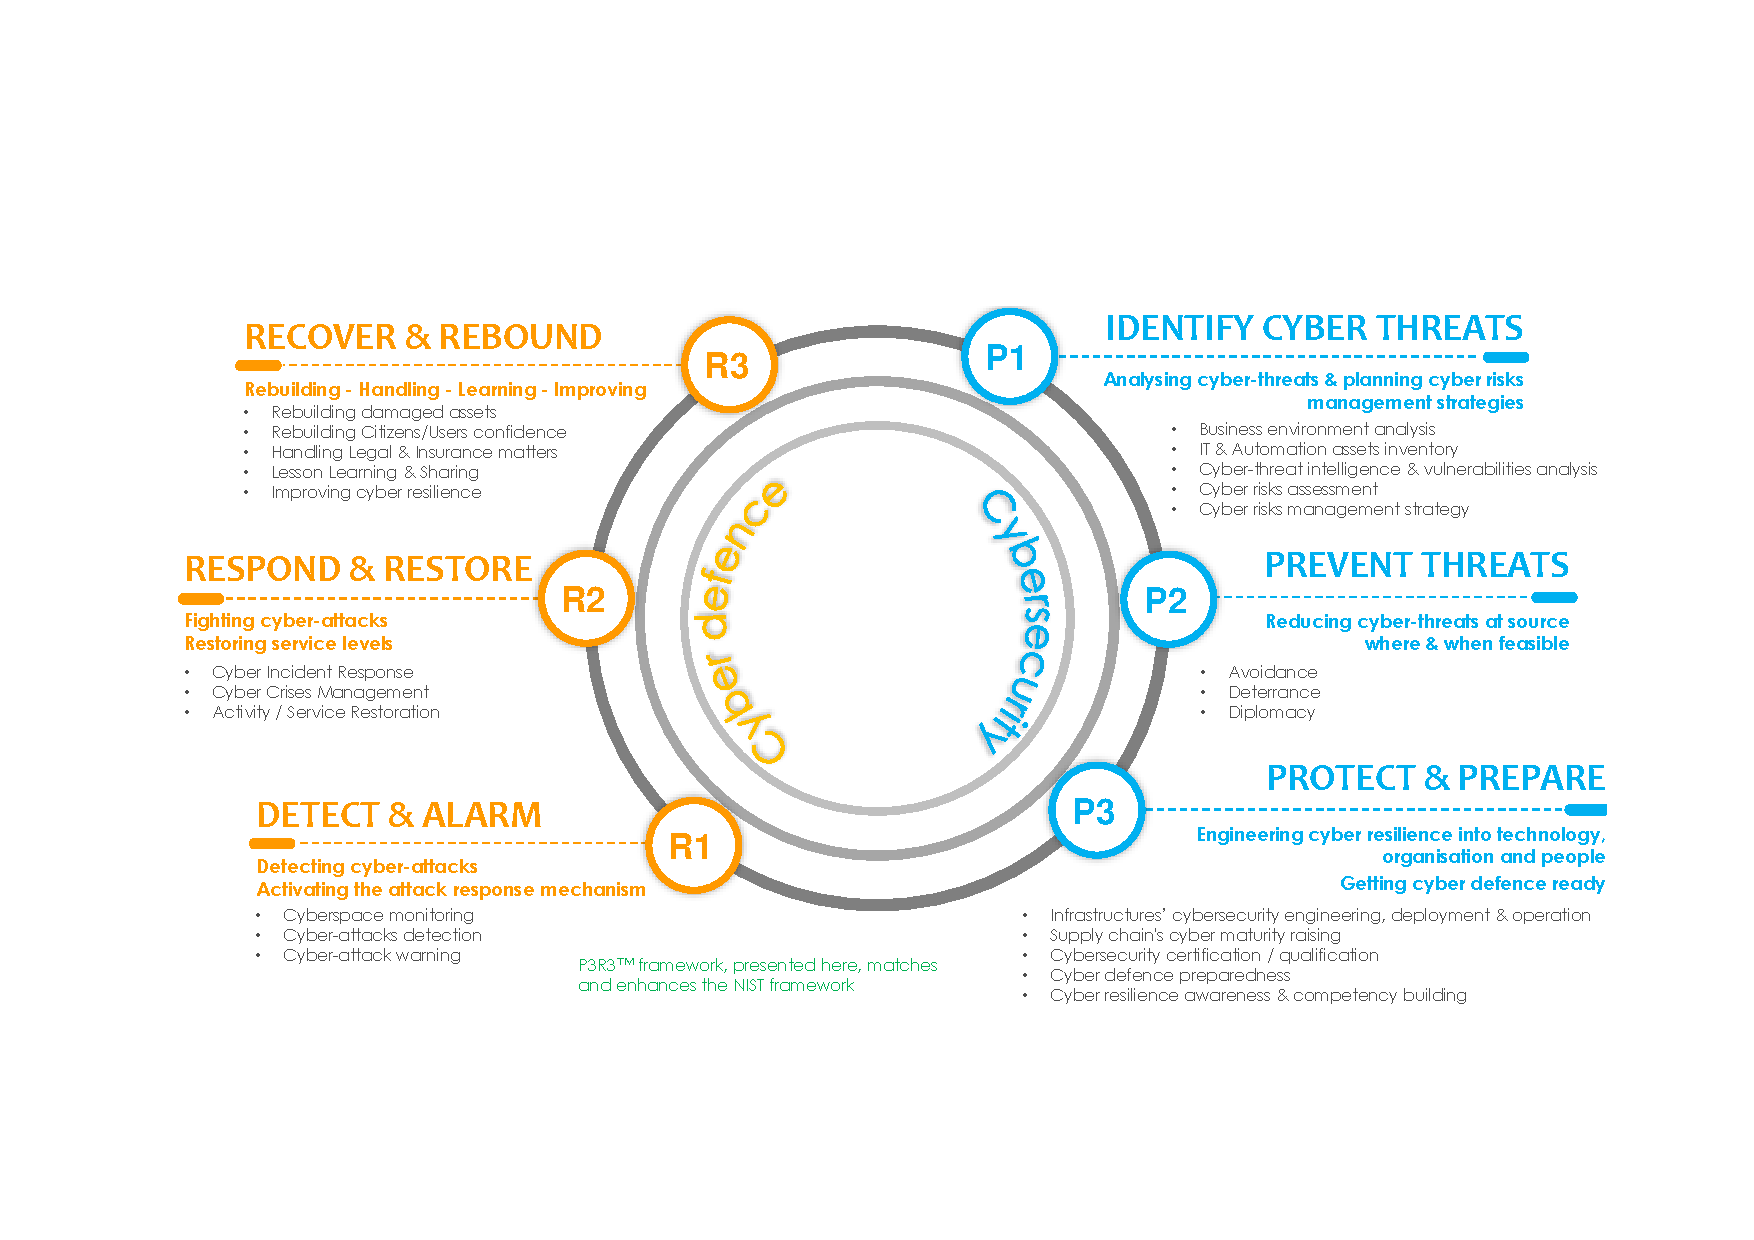
\includegraphics[width=\linewidth]{figures/P3R3.pdf}
  \caption{Le modèle P3R3 pour la cyber-résilience (tiré de \autocite{Kott2023})}
  \label{fig:P3R3_model}
\end{figure}

\noindent
L'essentiel de la Cyber-résilience repose sur une combinaison de détection  et de réponse face aux cybermenaces. Toutefois, l'émergence de menaces toujours plus rapides, distribuées et intelligentes remet en cause les approches traditionnelles. C'est ce que nous explorons dans la section suivante, en analysant les évolutions récentes du paysage des cyberattaques et les défis associés à leur détection et leur neutralisation.


\section{Des menaces de plus en plus autonomes et distribuées}\label{sec:evolution-menaces}

Au cours des dernières années, l'écosystème des cybermenaces a subi une transformation majeure. L'arrivée de l'\acn{IA} agentique permet l'émergence d'attaques plus rapides, automatisées, adaptatives et opèrant en parallèle non seulement sur un hôte unique, mais sur des réseaux entiers~\cite{Cohen2020}. Des travaux récents montrent que des attaquants utilisent des \acn{LLM} pour générer des malwares, créer des campagnes de phishing ciblées, et réagir d'eux-mêmes aux systèmes de défense~\cite{AutoAttacker2024}. De tels systèmes permettent de déclencher des campagnes distribuées avec une vitesse et une efficacité très importante~\cite{AgenticAIThreats2025}.

\subsection*{Limites des approches classiques de la Cyberdéfense}

Les dispositifs de Cyberdéfense traditionnels (fondés sur des architectures centralisées, des signatures statiques ou des règles prédéfinies) sont aujourd'hui dépassés par cette nouvelle génération de menaces~\cite{Kott2023}~:
\begin{itemize}
  \item \textbf{Latence décisionnelle}~: la centralisation de la détection engendre des délais critiques, permettant à certaines attaques de se produire avant même qu’elles ne soient identifiées et traitées par les équipes de Cyberdéfense~;
  \item \textbf{Rigidité adaptative}~: des règles statiques ne peuvent suivre l'évolution des modes opératoires des attaquants~;
  \item \textbf{Peu de résilience}~: lorsqu'une attaque est détectée, aucune action corrective immédiate n'est engagée. Cela retarde la restauration du système et laisse les conséquences de l'incident s'aggraver, limitant ainsi l'efficacité de la réponse post-attaque.
\end{itemize}

Ces limites identifiées soulignent la nécessité d'un paradigme plus agile, proactif et intelligent dans la Cyberdéfense. Des études récentes identifient l'avènement d'attaques basées sur l'\acn{IA}~\cite{Miles2018,AutoAttacker2024,Falong2025}, où les agents malveillants~:
\begin{itemize}
  \item \textbf{Automatisent} la recherche de vulnérabilités, le déploiement de charges utiles, et l'exfiltration~;
  \item \textbf{Coopèrent} en coordonnant des vecteurs d'attaque parallèles décrits dans les modèles de multi-agents adverses~;
  \item \textbf{Exploitent} des techniques d'\textbf{adversarial ML}, générant des formes d'échappement aux detections habituelles (poisoning, prompt injection…).
\end{itemize}

\subsection*{Une approche autonome de Cyberdéfense}

Pour faire face à ces menaces, le domaine émergent de l'\acn{ACO} cherche à développer des systèmes capables de prendre des décisions complexes de manière autonome, en tenant compte du contexte, des objectifs à atteindre et des conséquences possibles de leurs actions, le tout en temps réel et avec une supervision humaine minimale, voire inexistante~\cite{Vyas2023}. Les premiers travaux dans ce domaine portent principalement sur des architectures à base d'agents logiciels autonomes, en particulier dans le cadre du groupe \textit{IST-152} de l'\acn{OTAN}, à l'origine du concept d'agent \acn{AICA}.
Un tel agent est théorisé comme étant capable de percevoir son environnement local (par l'analyse de journaux, de flux ou d'heuristiques), de prendre des décisions autonomes en s'appuyant sur des règles ou des mécanismes d'apprentissage, d'agir localement (par exemple via des actions de filtrage ou d'isolement) sans dépendre d'un contrôle externe permanent, et enfin de communiquer avec d'autres agents ou des opérateurs humains afin de partager des indicateurs, des intentions ou des états.

Dans ce cadre, l'architecture modulaire \acn{MASCARA}, illustrée en \autoref{fig:mascara}, a été introduite pour formaliser le fonctionnement interne d'un agent \acn{AICA} en décomposant ses activités en plusieurs modules spécialisés~: collecte de journaux, détection d'anomalies, sélection de contre-mesures, application des réponses, etc. En s'appuyant sur cette architecture générale, il devient possible de concevoir une instance concrète adaptée à un environnement spécifique, en modulant le nombre de composants, leur nature et leurs interactions. Une telle adaptation permet à l'agent \acn{AICA} de répondre finement aux exigences de son contexte de déploiement et de garantir une protection {\em en edge}, c'est-à-dire au plus proche des ressources à défendre, tout en optimisant la performance dans l'atteinte des objectifs de Cyberdéfense.

Cependant, cette architecture reste fondamentalement monolithique et figée. Elle ne fournit pas, en l'état, les moyens d'adaptation nécessaires pour faire face aux dynamiques imprévisibles d'un environnement opérationnel réel, en particulier dans le cadre de systèmes distribués, complexes et fortement interactifs. Cette rigidité limite significativement la capacité d'un agent \acn{AICA} à réagir à l'émergence de nouvelles menaces ou à s'ajuster aux contraintes environnementales fluctuantes.


\begin{figure}[h!]
  \centering
  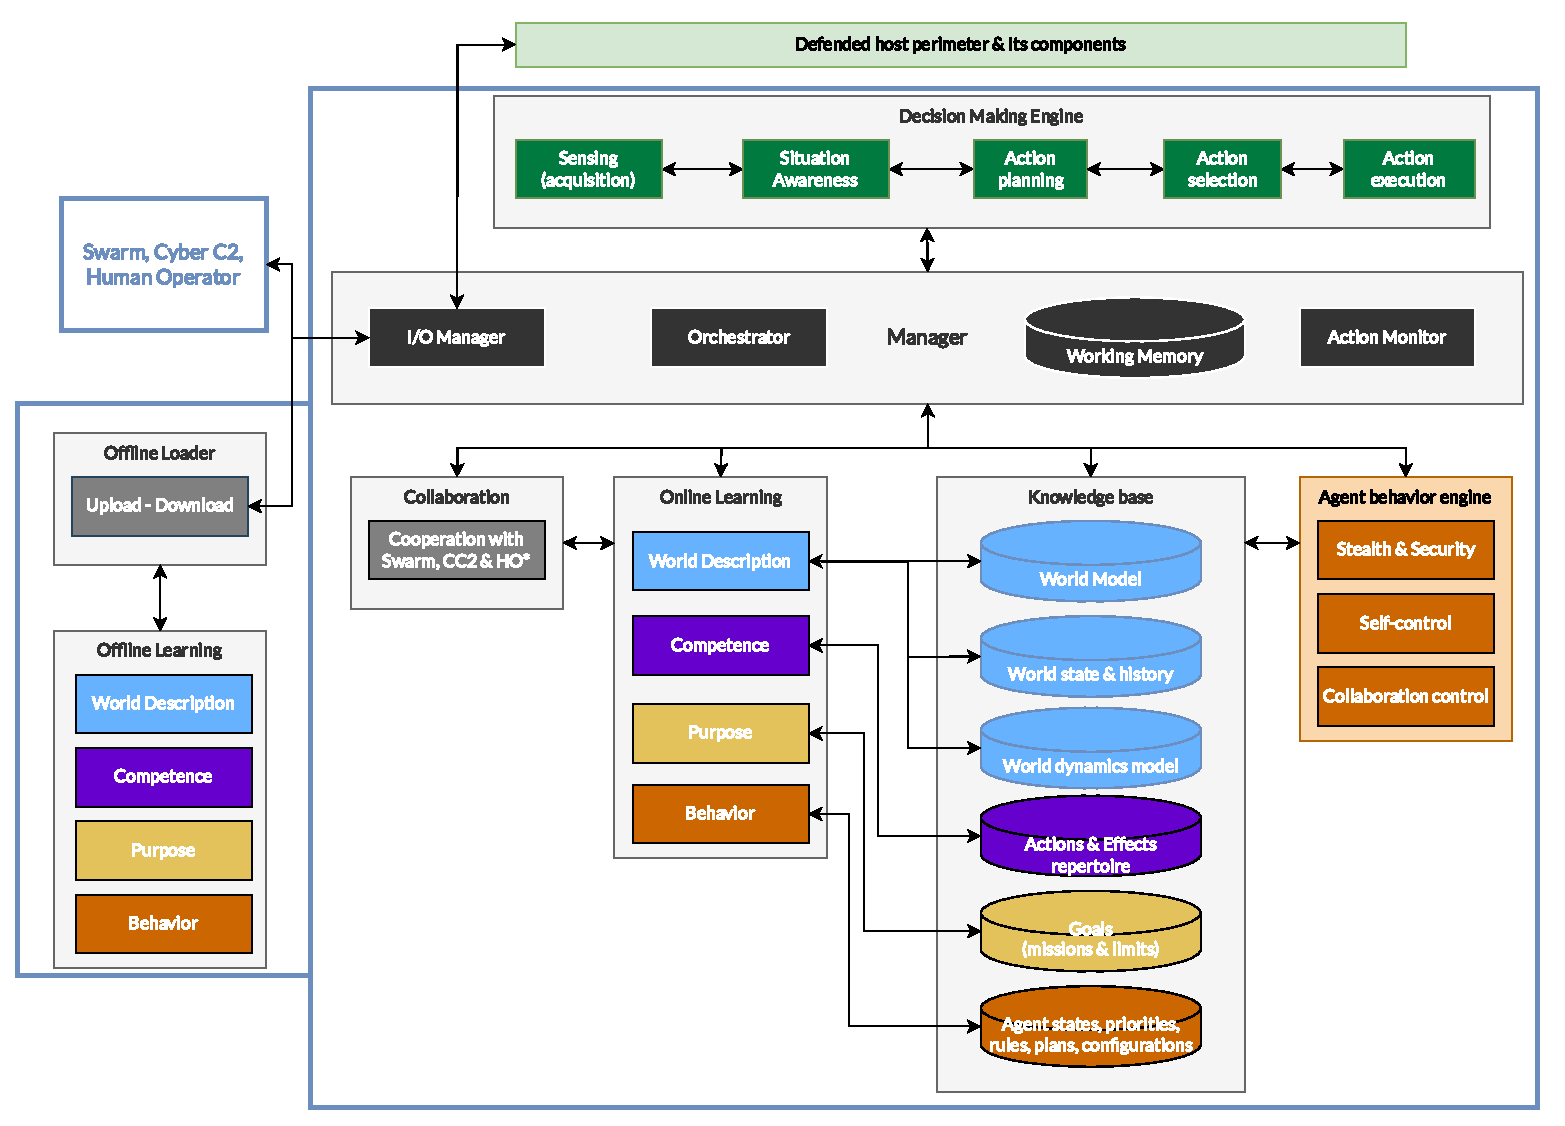
\includegraphics[width=\linewidth]{figures/MASCARA.pdf}
  \caption{Description de l'architecture modulaire MASCARA (tirée de \autocite{Kott2023})}
  \label{fig:mascara}
\end{figure}

\subsection*{Vers des approches coopératives}

La simple composition modulaire proposée initialement ne suffit plus à répondre à la complexité croissante des infrastructures critiques actuelles. Celle-ci impose l'adoption d'un paradigme distribué, dans lequel plusieurs agents interconnectés coopèrent, s'auto-organisent et se réorganisent dynamiquement en fonction des besoins opérationnels~\cite{Ferber1999, Gleizes2008}. Dans cette perspective, l'idée a émergé de transformer chaque module de l'architecture \acn{MASCARA} en un agent autonome, chargé d'exécuter une tâche spécifique de Cyberdéfense. Ces micro-agents, en interagissant de manière coordonnée, permettraient de mieux répartir les responsabilités, de renforcer la robustesse du système et d'atteindre collectivement les objectifs globaux de protection.

La notion de granularité permet ici d'opérer une distinction entre les micro-agents, chacun dédié à une fonction bien définie, et les agents \acn{AICA} dits complets, capables de couvrir l'ensemble des missions prévues par le modèle. Dans la suite de ce manuscrit, nous emploierons le terme générique d'agent \acn{AICA} pour désigner ces deux types d'agents, en précisant systématiquement le périmètre fonctionnel concerné selon le contexte.

Plus généralement, cette approche distribuée et coopérative s'inscrit dans une vision systémique de la Cyberdéfense, dans laquelle un ensemble d'agents autonomes interagit au sein du réseau pour garantir une sécurité globale, adaptative et résiliente. Cette orientation conceptuelle est soutenue par plusieurs travaux récents appartenant au domaine récent de l'\acn{ACD}~\cite{Vyas2023} (un sous domaine de l'\acparen{ACO}) et constitue un fondement essentiel des développements présentés dans ce manuscrit.


Par exemple, des simulations ont montré que des équipes d'agents défensifs sont capables de surpasser un agent unique en termes de couverture du réseau et de réactivité, grâce à une coordination dynamique et distribuée~\cite{RLResilientCyberdefense2024}.
Des plateformes telles que \textit{CybORG}~\cite{cage_challenge_3_announcement} illustrent également cette tendance, en proposant un environnement simulé dans lequel des agents autonomes décentralisés défendent simultanément un réseau face à des attaques coordonnées.

L'approche coopérative permet non seulement de protéger plusieurs hôtes en parallèle, mais aussi de détecter des attaques synchronisées et de s'adapter dynamiquement aux changements de topologie du réseau. Elle pose ainsi les bases d'une Cyberdéfense distribuée, proactive et évolutive, en rupture avec les architectures défensives traditionnelles.

\begin{figure}[h]
  \centering
  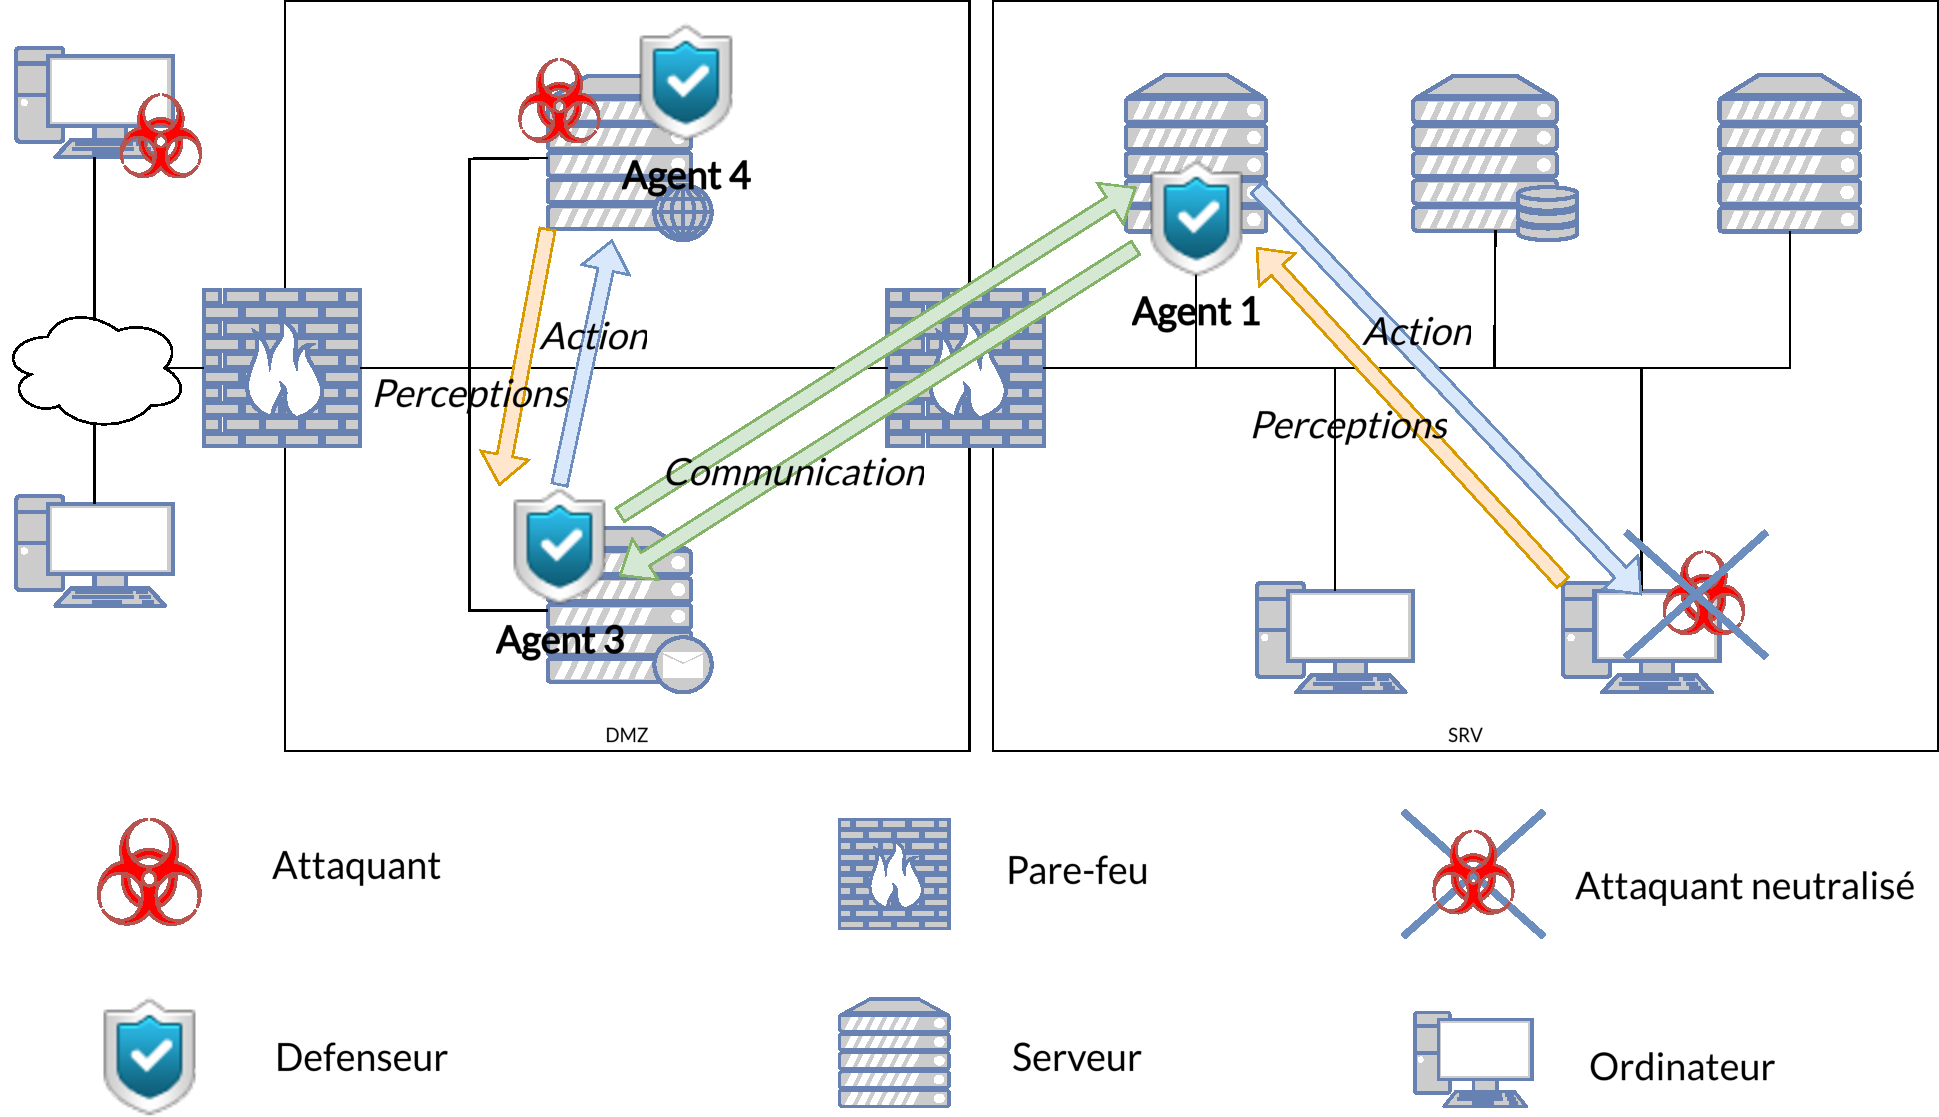
\includegraphics[width=\linewidth]{figures/infra_MAS_illustration.pdf}
  \caption{Illustration schématique d'un SMA de Cyberdéfense dans une infrastructure d'entreprise jouet}
  \label{fig:distributed_sma}
\end{figure}

\noindent
Finalement, c'est dans ce contexte que l'idée d'un \acn{SMA} de Cyberdéfense, tel que illustré dans \autoref{fig:distributed_sma}, apparaît comme une alternative générique prometteuse par rapport aux approches centralisées existantes. Nous présentons dans la section suivante les bases conceptuelles des \acn{SMA} en vue de la conception d'un \acn{SMA} de Cyberdéfense.

\section{La piste d'une vision multi-agent}\label{sec:sma-concepts}

Les \acn{SMA} constituent un paradigme central de l'\acn{IA} distribuée. Ils permettent de concevoir des systèmes complexes à partir d'agents autonomes interagissant dans un environnement partagé. Ces agents peuvent percevoir, raisonner, décider et agir de manière coordonnée pour résoudre des problèmes collectifs~\cite{Ferber1999,Wooldridge2002}.

\subsection*{Définitions fondamentales}

Un \textbf{agent} est une entité autonome, physique ou logicielle, capable de percevoir son environnement, de prendre des décisions et d'agir pour atteindre des objectifs~\cite{Russell2010}. Comme illustré dans \autoref{fig:sma_illustration}, un \acn{SMA} regroupe plusieurs de ces agents qui coopèrent ou interagissent au sein d’un environnement généralement dynamique et partiellement observable~\cite{Jennings1998,Shoham2007}. Chaque agent dispose d’une \emph{zone d’observation locale} (disque pointillé) lui permettant de percevoir uniquement une partie de l’environnement et des autres entités. À partir de ces observations partielles, et selon des \emph{stratégies ou politiques} (schéma en haut de la figure), il sélectionne et exécute des \emph{actions} dirigées vers des composants de l’environnement (carrés) ou vers d’autres agents (flèches pleines). Les agents peuvent également \emph{échanger des messages} (flèches en tirets) afin de coordonner leurs comportements. L’objectif global (en haut à droite) représente un état souhaité de l’environnement que les agents cherchent à atteindre collectivement.

\begin{figure}[h]
  \centering
  \resizebox{\textwidth}{!}{%
    


\tikzset{every picture/.style={line width=0.75pt}} %set default line width to 0.75pt        

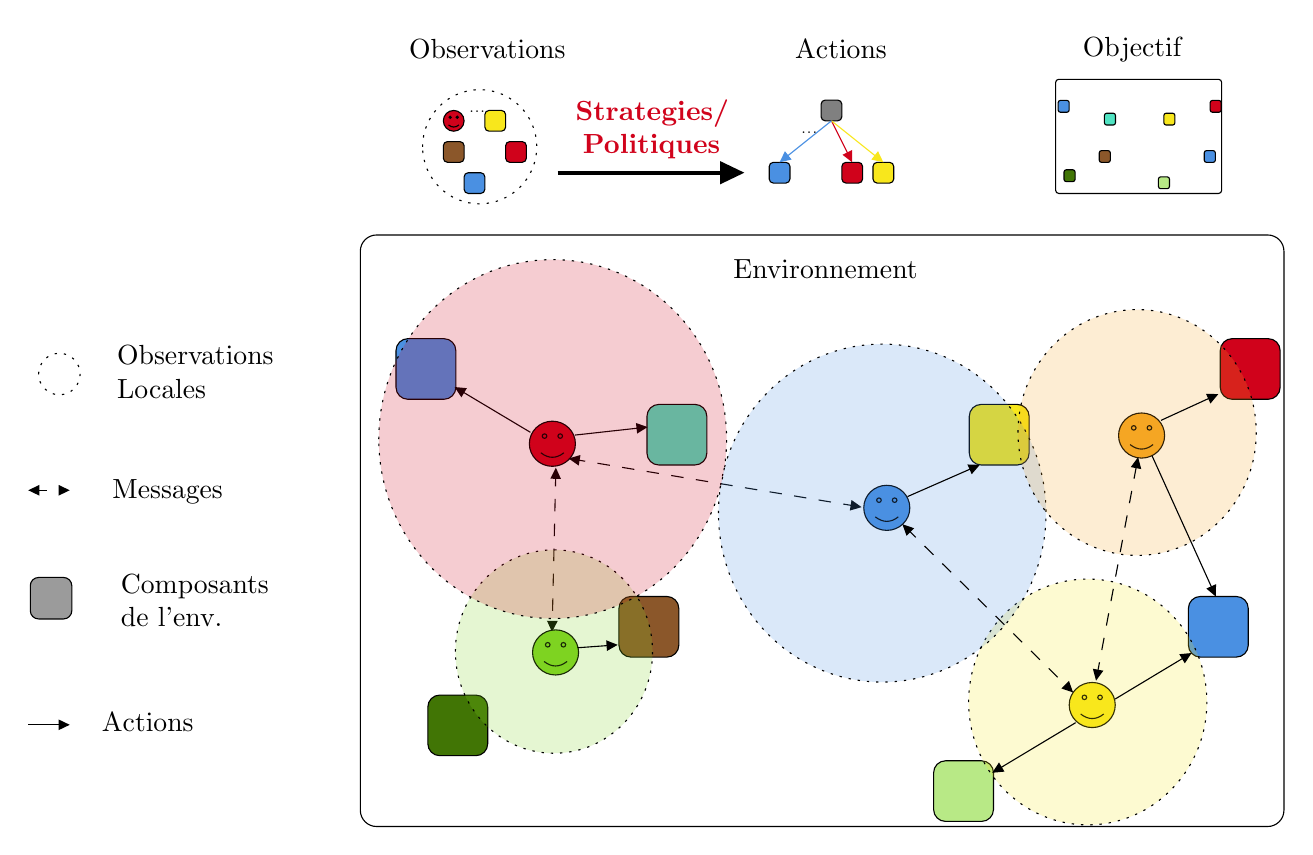
\begin{tikzpicture}[x=0.75pt,y=0.75pt,yscale=-1,xscale=1]
%uncomment if require: \path (0,1498); %set diagram left start at 0, and has height of 1498

%Rounded Rect [id:dp8571088761489256] 
\draw  [fill={rgb, 255:red, 255; green, 255; blue, 255 }  ,fill opacity=1 ] (195,482.84) .. controls (195,478.51) and (198.51,475) .. (202.84,475) -- (632.16,475) .. controls (636.49,475) and (640,478.51) .. (640,482.84) -- (640,752.16) .. controls (640,756.49) and (636.49,760) .. (632.16,760) -- (202.84,760) .. controls (198.51,760) and (195,756.49) .. (195,752.16) -- cycle ;
%Shape: Smiley Face [id:dp9608565483930217] 
\draw  [fill={rgb, 255:red, 208; green, 2; blue, 27 }  ,fill opacity=1 ] (276.44,575.59) .. controls (276.44,569.59) and (281.41,564.72) .. (287.53,564.72) .. controls (293.66,564.72) and (298.63,569.59) .. (298.63,575.59) .. controls (298.63,581.59) and (293.66,586.46) .. (287.53,586.46) .. controls (281.41,586.46) and (276.44,581.59) .. (276.44,575.59) -- cycle ; \draw  [fill={rgb, 255:red, 208; green, 2; blue, 27 }  ,fill opacity=1 ] (282.65,571.89) .. controls (282.65,571.29) and (283.15,570.81) .. (283.76,570.81) .. controls (284.37,570.81) and (284.87,571.29) .. (284.87,571.89) .. controls (284.87,572.49) and (284.37,572.98) .. (283.76,572.98) .. controls (283.15,572.98) and (282.65,572.49) .. (282.65,571.89) -- cycle ; \draw  [fill={rgb, 255:red, 208; green, 2; blue, 27 }  ,fill opacity=1 ] (290.2,571.89) .. controls (290.2,571.29) and (290.69,570.81) .. (291.31,570.81) .. controls (291.92,570.81) and (292.42,571.29) .. (292.42,571.89) .. controls (292.42,572.49) and (291.92,572.98) .. (291.31,572.98) .. controls (290.69,572.98) and (290.2,572.49) .. (290.2,571.89) -- cycle ; \draw   (281.99,579.94) .. controls (285.69,582.84) and (289.38,582.84) .. (293.08,579.94) ;
%Rounded Rect [id:dp759927621160896] 
\draw  [fill={rgb, 255:red, 80; green, 227; blue, 194 }  ,fill opacity=1 ] (333.1,562.39) .. controls (333.1,559.2) and (335.69,556.62) .. (338.87,556.62) -- (356.18,556.62) .. controls (359.37,556.62) and (361.95,559.2) .. (361.95,562.39) -- (361.95,580.06) .. controls (361.95,583.25) and (359.37,585.83) .. (356.18,585.83) -- (338.87,585.83) .. controls (335.69,585.83) and (333.1,583.25) .. (333.1,580.06) -- cycle ;
%Rounded Rect [id:dp3032709932069614] 
\draw  [fill={rgb, 255:red, 74; green, 144; blue, 226 }  ,fill opacity=1 ] (212.19,530.72) .. controls (212.19,527.54) and (214.77,524.95) .. (217.96,524.95) -- (235.26,524.95) .. controls (238.45,524.95) and (241.03,527.54) .. (241.03,530.72) -- (241.03,548.4) .. controls (241.03,551.58) and (238.45,554.17) .. (235.26,554.17) -- (217.96,554.17) .. controls (214.77,554.17) and (212.19,551.58) .. (212.19,548.4) -- cycle ;
%Straight Lines [id:da31697688905948296] 
\draw    (276.94,570.08) -- (243,549.8) ;
\draw [shift={(240.42,548.26)}, rotate = 30.86] [fill={rgb, 255:red, 0; green, 0; blue, 0 }  ][line width=0.08]  [draw opacity=0] (5.36,-2.57) -- (0,0) -- (5.36,2.57) -- cycle    ;
%Straight Lines [id:da15166297291059583] 
\draw  [dash pattern={on 4.5pt off 4.5pt}]  (289.15,590.12) -- (287.45,663.28) ;
\draw [shift={(287.38,666.28)}, rotate = 271.33] [fill={rgb, 255:red, 0; green, 0; blue, 0 }  ][line width=0.08]  [draw opacity=0] (5.36,-2.57) -- (0,0) -- (5.36,2.57) -- cycle    ;
\draw [shift={(289.22,587.12)}, rotate = 91.33] [fill={rgb, 255:red, 0; green, 0; blue, 0 }  ][line width=0.08]  [draw opacity=0] (5.36,-2.57) -- (0,0) -- (5.36,2.57) -- cycle    ;
%Straight Lines [id:da19030240516000207] 
\draw  [dash pattern={on 4.5pt off 4.5pt}]  (433.57,605.62) -- (298.31,583.17) ;
\draw [shift={(295.36,582.68)}, rotate = 9.42] [fill={rgb, 255:red, 0; green, 0; blue, 0 }  ][line width=0.08]  [draw opacity=0] (5.36,-2.57) -- (0,0) -- (5.36,2.57) -- cycle    ;
\draw [shift={(436.53,606.12)}, rotate = 189.42] [fill={rgb, 255:red, 0; green, 0; blue, 0 }  ][line width=0.08]  [draw opacity=0] (5.36,-2.57) -- (0,0) -- (5.36,2.57) -- cycle    ;
%Straight Lines [id:da12208855578128797] 
\draw    (298.42,571.41) -- (330.43,567.88) ;
\draw [shift={(333.41,567.55)}, rotate = 173.7] [fill={rgb, 255:red, 0; green, 0; blue, 0 }  ][line width=0.08]  [draw opacity=0] (5.36,-2.57) -- (0,0) -- (5.36,2.57) -- cycle    ;
%Shape: Smiley Face [id:dp017117759022491463] 
\draw  [fill={rgb, 255:red, 126; green, 211; blue, 33 }  ,fill opacity=1 ] (277.98,676.13) .. controls (277.98,670.13) and (282.94,665.26) .. (289.07,665.26) .. controls (295.2,665.26) and (300.16,670.13) .. (300.16,676.13) .. controls (300.16,682.13) and (295.2,687) .. (289.07,687) .. controls (282.94,687) and (277.98,682.13) .. (277.98,676.13) -- cycle ; \draw  [fill={rgb, 255:red, 126; green, 211; blue, 33 }  ,fill opacity=1 ] (284.19,672.44) .. controls (284.19,671.84) and (284.68,671.35) .. (285.3,671.35) .. controls (285.91,671.35) and (286.41,671.84) .. (286.41,672.44) .. controls (286.41,673.04) and (285.91,673.52) .. (285.3,673.52) .. controls (284.68,673.52) and (284.19,673.04) .. (284.19,672.44) -- cycle ; \draw  [fill={rgb, 255:red, 126; green, 211; blue, 33 }  ,fill opacity=1 ] (291.73,672.44) .. controls (291.73,671.84) and (292.23,671.35) .. (292.84,671.35) .. controls (293.45,671.35) and (293.95,671.84) .. (293.95,672.44) .. controls (293.95,673.04) and (293.45,673.52) .. (292.84,673.52) .. controls (292.23,673.52) and (291.73,673.04) .. (291.73,672.44) -- cycle ; \draw   (283.52,680.48) .. controls (287.22,683.38) and (290.92,683.38) .. (294.62,680.48) ;
%Rounded Rect [id:dp2729577267316856] 
\draw  [fill={rgb, 255:red, 65; green, 117; blue, 5 }  ,fill opacity=1 ] (227.53,702.44) .. controls (227.53,699.25) and (230.11,696.67) .. (233.3,696.67) -- (250.61,696.67) .. controls (253.8,696.67) and (256.38,699.25) .. (256.38,702.44) -- (256.38,720.11) .. controls (256.38,723.3) and (253.8,725.88) .. (250.61,725.88) -- (233.3,725.88) .. controls (230.11,725.88) and (227.53,723.3) .. (227.53,720.11) -- cycle ;
%Rounded Rect [id:dp9608207589356206] 
\draw  [fill={rgb, 255:red, 184; green, 233; blue, 134 }  ,fill opacity=1 ] (471.21,734.1) .. controls (471.21,730.92) and (473.79,728.33) .. (476.98,728.33) -- (494.29,728.33) .. controls (497.47,728.33) and (500.06,730.92) .. (500.06,734.1) -- (500.06,751.78) .. controls (500.06,754.96) and (497.47,757.55) .. (494.29,757.55) -- (476.98,757.55) .. controls (473.79,757.55) and (471.21,754.96) .. (471.21,751.78) -- cycle ;
%Rounded Rect [id:dp2532918382479751] 
\draw  [fill={rgb, 255:red, 248; green, 231; blue, 28 }  ,fill opacity=1 ] (488.39,562.39) .. controls (488.39,559.2) and (490.98,556.62) .. (494.16,556.62) -- (511.47,556.62) .. controls (514.66,556.62) and (517.24,559.2) .. (517.24,562.39) -- (517.24,580.06) .. controls (517.24,583.25) and (514.66,585.83) .. (511.47,585.83) -- (494.16,585.83) .. controls (490.98,585.83) and (488.39,583.25) .. (488.39,580.06) -- cycle ;
%Rounded Rect [id:dp46841976175690214] 
\draw  [fill={rgb, 255:red, 74; green, 144; blue, 226 }  ,fill opacity=1 ] (593.97,654.94) .. controls (593.97,651.75) and (596.55,649.17) .. (599.74,649.17) -- (617.04,649.17) .. controls (620.23,649.17) and (622.81,651.75) .. (622.81,654.94) -- (622.81,672.61) .. controls (622.81,675.8) and (620.23,678.38) .. (617.04,678.38) -- (599.74,678.38) .. controls (596.55,678.38) and (593.97,675.8) .. (593.97,672.61) -- cycle ;
%Rounded Rect [id:dp35096543230819477] 
\draw  [fill={rgb, 255:red, 208; green, 2; blue, 27 }  ,fill opacity=1 ] (609.31,530.72) .. controls (609.31,527.54) and (611.89,524.95) .. (615.08,524.95) -- (632.39,524.95) .. controls (635.58,524.95) and (638.16,527.54) .. (638.16,530.72) -- (638.16,548.4) .. controls (638.16,551.58) and (635.58,554.17) .. (632.39,554.17) -- (615.08,554.17) .. controls (611.89,554.17) and (609.31,551.58) .. (609.31,548.4) -- cycle ;
%Rounded Rect [id:dp37268226656767] 
\draw  [fill={rgb, 255:red, 139; green, 87; blue, 42 }  ,fill opacity=1 ] (319.6,654.94) .. controls (319.6,651.75) and (322.18,649.17) .. (325.37,649.17) -- (342.68,649.17) .. controls (345.87,649.17) and (348.45,651.75) .. (348.45,654.94) -- (348.45,672.61) .. controls (348.45,675.8) and (345.87,678.38) .. (342.68,678.38) -- (325.37,678.38) .. controls (322.18,678.38) and (319.6,675.8) .. (319.6,672.61) -- cycle ;
%Shape: Smiley Face [id:dp8112481576921686] 
\draw  [fill={rgb, 255:red, 245; green, 166; blue, 35 }  ,fill opacity=1 ] (560.32,571.63) .. controls (560.32,565.63) and (565.29,560.76) .. (571.41,560.76) .. controls (577.54,560.76) and (582.51,565.63) .. (582.51,571.63) .. controls (582.51,577.63) and (577.54,582.5) .. (571.41,582.5) .. controls (565.29,582.5) and (560.32,577.63) .. (560.32,571.63) -- cycle ; \draw  [fill={rgb, 255:red, 245; green, 166; blue, 35 }  ,fill opacity=1 ] (566.53,567.94) .. controls (566.53,567.34) and (567.03,566.85) .. (567.64,566.85) .. controls (568.25,566.85) and (568.75,567.34) .. (568.75,567.94) .. controls (568.75,568.54) and (568.25,569.02) .. (567.64,569.02) .. controls (567.03,569.02) and (566.53,568.54) .. (566.53,567.94) -- cycle ; \draw  [fill={rgb, 255:red, 245; green, 166; blue, 35 }  ,fill opacity=1 ] (574.08,567.94) .. controls (574.08,567.34) and (574.57,566.85) .. (575.19,566.85) .. controls (575.8,566.85) and (576.29,567.34) .. (576.29,567.94) .. controls (576.29,568.54) and (575.8,569.02) .. (575.19,569.02) .. controls (574.57,569.02) and (574.08,568.54) .. (574.08,567.94) -- cycle ; \draw   (565.87,575.98) .. controls (569.56,578.88) and (573.26,578.88) .. (576.96,575.98) ;
%Shape: Smiley Face [id:dp26692841414623936] 
\draw  [fill={rgb, 255:red, 248; green, 231; blue, 28 }  ,fill opacity=1 ] (536.54,701.46) .. controls (536.54,695.46) and (541.5,690.6) .. (547.63,690.6) .. controls (553.76,690.6) and (558.72,695.46) .. (558.72,701.46) .. controls (558.72,707.47) and (553.76,712.33) .. (547.63,712.33) .. controls (541.5,712.33) and (536.54,707.47) .. (536.54,701.46) -- cycle ; \draw  [fill={rgb, 255:red, 248; green, 231; blue, 28 }  ,fill opacity=1 ] (542.75,697.77) .. controls (542.75,697.17) and (543.24,696.68) .. (543.86,696.68) .. controls (544.47,696.68) and (544.97,697.17) .. (544.97,697.77) .. controls (544.97,698.37) and (544.47,698.86) .. (543.86,698.86) .. controls (543.24,698.86) and (542.75,698.37) .. (542.75,697.77) -- cycle ; \draw  [fill={rgb, 255:red, 248; green, 231; blue, 28 }  ,fill opacity=1 ] (550.29,697.77) .. controls (550.29,697.17) and (550.79,696.68) .. (551.4,696.68) .. controls (552.01,696.68) and (552.51,697.17) .. (552.51,697.77) .. controls (552.51,698.37) and (552.01,698.86) .. (551.4,698.86) .. controls (550.79,698.86) and (550.29,698.37) .. (550.29,697.77) -- cycle ; \draw   (542.08,705.81) .. controls (545.78,708.71) and (549.48,708.71) .. (553.18,705.81) ;
%Shape: Smiley Face [id:dp13683684589232226] 
\draw  [fill={rgb, 255:red, 74; green, 144; blue, 226 }  ,fill opacity=1 ] (437.56,606.46) .. controls (437.56,600.46) and (442.53,595.6) .. (448.65,595.6) .. controls (454.78,595.6) and (459.75,600.46) .. (459.75,606.46) .. controls (459.75,612.47) and (454.78,617.33) .. (448.65,617.33) .. controls (442.53,617.33) and (437.56,612.47) .. (437.56,606.46) -- cycle ; \draw  [fill={rgb, 255:red, 74; green, 144; blue, 226 }  ,fill opacity=1 ] (443.77,602.77) .. controls (443.77,602.17) and (444.27,601.68) .. (444.88,601.68) .. controls (445.5,601.68) and (445.99,602.17) .. (445.99,602.77) .. controls (445.99,603.37) and (445.5,603.86) .. (444.88,603.86) .. controls (444.27,603.86) and (443.77,603.37) .. (443.77,602.77) -- cycle ; \draw  [fill={rgb, 255:red, 74; green, 144; blue, 226 }  ,fill opacity=1 ] (451.32,602.77) .. controls (451.32,602.17) and (451.81,601.68) .. (452.43,601.68) .. controls (453.04,601.68) and (453.54,602.17) .. (453.54,602.77) .. controls (453.54,603.37) and (453.04,603.86) .. (452.43,603.86) .. controls (451.81,603.86) and (451.32,603.37) .. (451.32,602.77) -- cycle ; \draw   (443.11,610.81) .. controls (446.81,613.71) and (450.5,613.71) .. (454.2,610.81) ;
%Shape: Ellipse [id:dp20697299562525007] 
\draw  [fill={rgb, 255:red, 126; green, 211; blue, 33 }  ,fill opacity=0.2 ][dash pattern={on 0.84pt off 2.51pt}] (240.81,675.7) .. controls (240.81,648.64) and (262.07,626.7) .. (288.3,626.7) .. controls (314.52,626.7) and (335.79,648.64) .. (335.79,675.7) .. controls (335.79,702.76) and (314.52,724.7) .. (288.3,724.7) .. controls (262.07,724.7) and (240.81,702.76) .. (240.81,675.7) -- cycle ;
%Shape: Ellipse [id:dp5331145075645709] 
\draw  [fill={rgb, 255:red, 248; green, 231; blue, 28 }  ,fill opacity=0.2 ][dash pattern={on 0.84pt off 2.51pt}] (488.09,699.99) .. controls (488.09,667.29) and (513.78,640.78) .. (545.47,640.78) .. controls (577.17,640.78) and (602.86,667.29) .. (602.86,699.99) .. controls (602.86,732.7) and (577.17,759.21) .. (545.47,759.21) .. controls (513.78,759.21) and (488.09,732.7) .. (488.09,699.99) -- cycle ;
%Shape: Ellipse [id:dp1108681712787154] 
\draw  [fill={rgb, 255:red, 74; green, 144; blue, 226 }  ,fill opacity=0.2 ][dash pattern={on 0.84pt off 2.51pt}] (367.55,608.99) .. controls (367.55,564.02) and (402.88,527.57) .. (446.46,527.57) .. controls (490.04,527.57) and (525.37,564.02) .. (525.37,608.99) .. controls (525.37,653.96) and (490.04,690.41) .. (446.46,690.41) .. controls (402.88,690.41) and (367.55,653.96) .. (367.55,608.99) -- cycle ;
%Shape: Ellipse [id:dp35349211767213196] 
\draw  [fill={rgb, 255:red, 245; green, 166; blue, 35 }  ,fill opacity=0.2 ][dash pattern={on 0.84pt off 2.51pt}] (511.87,570.16) .. controls (511.87,537.46) and (537.56,510.95) .. (569.26,510.95) .. controls (600.95,510.95) and (626.65,537.46) .. (626.65,570.16) .. controls (626.65,602.86) and (600.95,629.38) .. (569.26,629.38) .. controls (537.56,629.38) and (511.87,602.86) .. (511.87,570.16) -- cycle ;
%Straight Lines [id:da868926834515953] 
\draw    (299.65,673.88) -- (315.99,672.69) ;
\draw [shift={(318.99,672.47)}, rotate = 175.83] [fill={rgb, 255:red, 0; green, 0; blue, 0 }  ][line width=0.08]  [draw opacity=0] (5.36,-2.57) -- (0,0) -- (5.36,2.57) -- cycle    ;
%Straight Lines [id:da7856168052805825] 
\draw    (458.62,601.05) -- (490.69,586.98) ;
\draw [shift={(493.44,585.77)}, rotate = 156.31] [fill={rgb, 255:red, 0; green, 0; blue, 0 }  ][line width=0.08]  [draw opacity=0] (5.36,-2.57) -- (0,0) -- (5.36,2.57) -- cycle    ;
%Straight Lines [id:da9445808525599552] 
\draw    (580.77,564.32) -- (605.66,552.9) ;
\draw [shift={(608.39,551.65)}, rotate = 155.36] [fill={rgb, 255:red, 0; green, 0; blue, 0 }  ][line width=0.08]  [draw opacity=0] (5.36,-2.57) -- (0,0) -- (5.36,2.57) -- cycle    ;
%Straight Lines [id:da12131692830119956] 
\draw    (558.67,698.58) -- (592.93,677.96) ;
\draw [shift={(595.5,676.42)}, rotate = 148.96] [fill={rgb, 255:red, 0; green, 0; blue, 0 }  ][line width=0.08]  [draw opacity=0] (5.36,-2.57) -- (0,0) -- (5.36,2.57) -- cycle    ;
%Straight Lines [id:da02866326716436185] 
\draw    (539.64,709.98) -- (502.01,732.57) ;
\draw [shift={(499.44,734.11)}, rotate = 329.03] [fill={rgb, 255:red, 0; green, 0; blue, 0 }  ][line width=0.08]  [draw opacity=0] (5.36,-2.57) -- (0,0) -- (5.36,2.57) -- cycle    ;
%Straight Lines [id:da3852011537026049] 
\draw  [dash pattern={on 4.5pt off 4.5pt}]  (458.31,616.46) -- (536.28,693.31) ;
\draw [shift={(538.42,695.42)}, rotate = 224.59] [fill={rgb, 255:red, 0; green, 0; blue, 0 }  ][line width=0.08]  [draw opacity=0] (5.36,-2.57) -- (0,0) -- (5.36,2.57) -- cycle    ;
\draw [shift={(456.17,614.35)}, rotate = 44.59] [fill={rgb, 255:red, 0; green, 0; blue, 0 }  ][line width=0.08]  [draw opacity=0] (5.36,-2.57) -- (0,0) -- (5.36,2.57) -- cycle    ;
%Straight Lines [id:da9204270310799157] 
\draw  [dash pattern={on 4.5pt off 4.5pt}]  (550.02,686.77) -- (569.17,585) ;
\draw [shift={(569.72,582.05)}, rotate = 100.65] [fill={rgb, 255:red, 0; green, 0; blue, 0 }  ][line width=0.08]  [draw opacity=0] (5.36,-2.57) -- (0,0) -- (5.36,2.57) -- cycle    ;
\draw [shift={(549.47,689.72)}, rotate = 280.65] [fill={rgb, 255:red, 0; green, 0; blue, 0 }  ][line width=0.08]  [draw opacity=0] (5.36,-2.57) -- (0,0) -- (5.36,2.57) -- cycle    ;
%Straight Lines [id:da9548969852220758] 
\draw    (576.47,581.42) -- (605.92,646.45) ;
\draw [shift={(607.16,649.18)}, rotate = 245.64] [fill={rgb, 255:red, 0; green, 0; blue, 0 }  ][line width=0.08]  [draw opacity=0] (5.36,-2.57) -- (0,0) -- (5.36,2.57) -- cycle    ;
%Shape: Ellipse [id:dp5345394122462545] 
\draw  [fill={rgb, 255:red, 208; green, 2; blue, 27 }  ,fill opacity=0.2 ][dash pattern={on 0.84pt off 2.51pt}] (203.9,573.33) .. controls (203.9,525.58) and (241.41,486.88) .. (287.68,486.88) .. controls (333.95,486.88) and (371.47,525.58) .. (371.47,573.33) .. controls (371.47,621.07) and (333.95,659.78) .. (287.68,659.78) .. controls (241.41,659.78) and (203.9,621.07) .. (203.9,573.33) -- cycle ;
%Rounded Rect [id:dp14561871899929513] 
\draw  [fill={rgb, 255:red, 155; green, 155; blue, 155 }  ,fill opacity=1 ] (36,644) .. controls (36,641.79) and (37.79,640) .. (40,640) -- (52,640) .. controls (54.21,640) and (56,641.79) .. (56,644) -- (56,656) .. controls (56,658.21) and (54.21,660) .. (52,660) -- (40,660) .. controls (37.79,660) and (36,658.21) .. (36,656) -- cycle ;
%Shape: Circle [id:dp8389216043634751] 
\draw  [dash pattern={on 0.84pt off 2.51pt}] (40,542) .. controls (40,536.48) and (44.48,532) .. (50,532) .. controls (55.52,532) and (60,536.48) .. (60,542) .. controls (60,547.52) and (55.52,552) .. (50,552) .. controls (44.48,552) and (40,547.52) .. (40,542) -- cycle ;
%Rounded Rect [id:dp1716372782625939] 
\draw  [fill={rgb, 255:red, 255; green, 255; blue, 255 }  ,fill opacity=1 ] (530,401.51) .. controls (530,400.68) and (530.68,400) .. (531.51,400) -- (608.49,400) .. controls (609.32,400) and (610,400.68) .. (610,401.51) -- (610,453.49) .. controls (610,454.32) and (609.32,455) .. (608.49,455) -- (531.51,455) .. controls (530.68,455) and (530,454.32) .. (530,453.49) -- cycle ;
%Rounded Rect [id:dp8384348356925067] 
\draw  [fill={rgb, 255:red, 80; green, 227; blue, 194 }  ,fill opacity=1 ] (553.51,417.41) .. controls (553.51,416.82) and (553.99,416.34) .. (554.57,416.34) -- (557.77,416.34) .. controls (558.35,416.34) and (558.83,416.82) .. (558.83,417.41) -- (558.83,420.96) .. controls (558.83,421.55) and (558.35,422.03) .. (557.77,422.03) -- (554.57,422.03) .. controls (553.99,422.03) and (553.51,421.55) .. (553.51,420.96) -- cycle ;
%Rounded Rect [id:dp32115157665477156] 
\draw  [fill={rgb, 255:red, 65; green, 117; blue, 5 }  ,fill opacity=1 ] (534.04,444.66) .. controls (534.04,444.07) and (534.52,443.59) .. (535.1,443.59) -- (538.3,443.59) .. controls (538.88,443.59) and (539.36,444.07) .. (539.36,444.66) -- (539.36,448.21) .. controls (539.36,448.8) and (538.88,449.28) .. (538.3,449.28) -- (535.1,449.28) .. controls (534.52,449.28) and (534.04,448.8) .. (534.04,448.21) -- cycle ;
%Rounded Rect [id:dp8306304589808061] 
\draw  [fill={rgb, 255:red, 184; green, 233; blue, 134 }  ,fill opacity=1 ] (579.52,448.07) .. controls (579.52,447.48) and (580,447) .. (580.59,447) -- (583.78,447) .. controls (584.37,447) and (584.84,447.48) .. (584.84,448.07) -- (584.84,451.62) .. controls (584.84,452.21) and (584.37,452.69) .. (583.78,452.69) -- (580.59,452.69) .. controls (580,452.69) and (579.52,452.21) .. (579.52,451.62) -- cycle ;
%Rounded Rect [id:dp36124132336547066] 
\draw  [fill={rgb, 255:red, 248; green, 231; blue, 28 }  ,fill opacity=1 ] (582.15,417.41) .. controls (582.15,416.82) and (582.63,416.34) .. (583.21,416.34) -- (586.41,416.34) .. controls (586.99,416.34) and (587.47,416.82) .. (587.47,417.41) -- (587.47,420.96) .. controls (587.47,421.55) and (586.99,422.03) .. (586.41,422.03) -- (583.21,422.03) .. controls (582.63,422.03) and (582.15,421.55) .. (582.15,420.96) -- cycle ;
%Rounded Rect [id:dp07486815562281168] 
\draw  [fill={rgb, 255:red, 74; green, 144; blue, 226 }  ,fill opacity=1 ] (601.62,435.41) .. controls (601.62,434.83) and (602.1,434.35) .. (602.68,434.35) -- (605.88,434.35) .. controls (606.46,434.35) and (606.94,434.83) .. (606.94,435.41) -- (606.94,438.97) .. controls (606.94,439.56) and (606.46,440.03) .. (605.88,440.03) -- (602.68,440.03) .. controls (602.1,440.03) and (601.62,439.56) .. (601.62,438.97) -- cycle ;
%Rounded Rect [id:dp30447435501798137] 
\draw  [fill={rgb, 255:red, 74; green, 144; blue, 226 }  ,fill opacity=1 ] (531.21,411.24) .. controls (531.21,410.66) and (531.69,410.18) .. (532.27,410.18) -- (535.47,410.18) .. controls (536.05,410.18) and (536.53,410.66) .. (536.53,411.24) -- (536.53,414.8) .. controls (536.53,415.39) and (536.05,415.86) .. (535.47,415.86) -- (532.27,415.86) .. controls (531.69,415.86) and (531.21,415.39) .. (531.21,414.8) -- cycle ;
%Rounded Rect [id:dp9375364402563595] 
\draw  [fill={rgb, 255:red, 208; green, 2; blue, 27 }  ,fill opacity=1 ] (604.45,411.24) .. controls (604.45,410.66) and (604.93,410.18) .. (605.51,410.18) -- (608.71,410.18) .. controls (609.29,410.18) and (609.77,410.66) .. (609.77,411.24) -- (609.77,414.8) .. controls (609.77,415.39) and (609.29,415.86) .. (608.71,415.86) -- (605.51,415.86) .. controls (604.93,415.86) and (604.45,415.39) .. (604.45,414.8) -- cycle ;
%Rounded Rect [id:dp7769696093588394] 
\draw  [fill={rgb, 255:red, 139; green, 87; blue, 42 }  ,fill opacity=1 ] (551.02,435.41) .. controls (551.02,434.83) and (551.5,434.35) .. (552.08,434.35) -- (555.28,434.35) .. controls (555.86,434.35) and (556.34,434.83) .. (556.34,435.41) -- (556.34,438.97) .. controls (556.34,439.56) and (555.86,440.03) .. (555.28,440.03) -- (552.08,440.03) .. controls (551.5,440.03) and (551.02,439.56) .. (551.02,438.97) -- cycle ;
%Straight Lines [id:da7689335282153781] 
\draw    (35,711) -- (52,711) ;
\draw [shift={(55,711)}, rotate = 180] [fill={rgb, 255:red, 0; green, 0; blue, 0 }  ][line width=0.08]  [draw opacity=0] (5.36,-2.57) -- (0,0) -- (5.36,2.57) -- cycle    ;
%Shape: Boxed Line [id:dp5305044082643576] 
\draw  [dash pattern={on 4.5pt off 4.5pt}]  (38,598) -- (52,598) ;
\draw [shift={(55,598)}, rotate = 180] [fill={rgb, 255:red, 0; green, 0; blue, 0 }  ][line width=0.08]  [draw opacity=0] (5.36,-2.57) -- (0,0) -- (5.36,2.57) -- cycle    ;
\draw [shift={(35,598)}, rotate = 0] [fill={rgb, 255:red, 0; green, 0; blue, 0 }  ][line width=0.08]  [draw opacity=0] (5.36,-2.57) -- (0,0) -- (5.36,2.57) -- cycle    ;
%Rounded Rect [id:dp4866637287235507] 
\draw  [fill={rgb, 255:red, 128; green, 128; blue, 128 }  ,fill opacity=1 ] (417,412) .. controls (417,410.9) and (417.9,410) .. (419,410) -- (425,410) .. controls (426.1,410) and (427,410.9) .. (427,412) -- (427,418) .. controls (427,419.1) and (426.1,420) .. (425,420) -- (419,420) .. controls (417.9,420) and (417,419.1) .. (417,418) -- cycle ;
%Rounded Rect [id:dp6679922716487737] 
\draw  [fill={rgb, 255:red, 74; green, 144; blue, 226 }  ,fill opacity=1 ] (392,442) .. controls (392,440.9) and (392.9,440) .. (394,440) -- (400,440) .. controls (401.1,440) and (402,440.9) .. (402,442) -- (402,448) .. controls (402,449.1) and (401.1,450) .. (400,450) -- (394,450) .. controls (392.9,450) and (392,449.1) .. (392,448) -- cycle ;
%Rounded Rect [id:dp6398718898903711] 
\draw  [fill={rgb, 255:red, 208; green, 2; blue, 27 }  ,fill opacity=1 ] (427,442) .. controls (427,440.9) and (427.9,440) .. (429,440) -- (435,440) .. controls (436.1,440) and (437,440.9) .. (437,442) -- (437,448) .. controls (437,449.1) and (436.1,450) .. (435,450) -- (429,450) .. controls (427.9,450) and (427,449.1) .. (427,448) -- cycle ;
%Straight Lines [id:da4441060393578834] 
\draw [color={rgb, 255:red, 208; green, 2; blue, 27 }  ,draw opacity=1 ]   (422,420) -- (430.66,437.32) ;
\draw [shift={(432,440)}, rotate = 243.43] [fill={rgb, 255:red, 208; green, 2; blue, 27 }  ,fill opacity=1 ][line width=0.08]  [draw opacity=0] (5.36,-2.57) -- (0,0) -- (5.36,2.57) -- cycle    ;
%Rounded Rect [id:dp08606049626209744] 
\draw  [fill={rgb, 255:red, 248; green, 231; blue, 28 }  ,fill opacity=1 ] (442,442) .. controls (442,440.9) and (442.9,440) .. (444,440) -- (450,440) .. controls (451.1,440) and (452,440.9) .. (452,442) -- (452,448) .. controls (452,449.1) and (451.1,450) .. (450,450) -- (444,450) .. controls (442.9,450) and (442,449.1) .. (442,448) -- cycle ;
%Straight Lines [id:da5780422632856335] 
\draw [color={rgb, 255:red, 248; green, 231; blue, 28 }  ,draw opacity=1 ]   (422,420) -- (444.66,438.13) ;
\draw [shift={(447,440)}, rotate = 218.66] [fill={rgb, 255:red, 248; green, 231; blue, 28 }  ,fill opacity=1 ][line width=0.08]  [draw opacity=0] (5.36,-2.57) -- (0,0) -- (5.36,2.57) -- cycle    ;
%Straight Lines [id:da6560295978621367] 
\draw [color={rgb, 255:red, 74; green, 144; blue, 226 }  ,draw opacity=1 ]   (422,420) -- (399.34,438.13) ;
\draw [shift={(397,440)}, rotate = 321.34] [fill={rgb, 255:red, 74; green, 144; blue, 226 }  ,fill opacity=1 ][line width=0.08]  [draw opacity=0] (5.36,-2.57) -- (0,0) -- (5.36,2.57) -- cycle    ;
%Rounded Rect [id:dp8389325005978227] 
\draw  [fill={rgb, 255:red, 139; green, 87; blue, 42 }  ,fill opacity=1 ] (235,432) .. controls (235,430.9) and (235.9,430) .. (237,430) -- (243,430) .. controls (244.1,430) and (245,430.9) .. (245,432) -- (245,438) .. controls (245,439.1) and (244.1,440) .. (243,440) -- (237,440) .. controls (235.9,440) and (235,439.1) .. (235,438) -- cycle ;
%Rounded Rect [id:dp11911600050294124] 
\draw  [fill={rgb, 255:red, 74; green, 144; blue, 226 }  ,fill opacity=1 ] (245,447) .. controls (245,445.9) and (245.9,445) .. (247,445) -- (253,445) .. controls (254.1,445) and (255,445.9) .. (255,447) -- (255,453) .. controls (255,454.1) and (254.1,455) .. (253,455) -- (247,455) .. controls (245.9,455) and (245,454.1) .. (245,453) -- cycle ;
%Rounded Rect [id:dp6632279611422938] 
\draw  [fill={rgb, 255:red, 248; green, 231; blue, 28 }  ,fill opacity=1 ] (255,417) .. controls (255,415.9) and (255.9,415) .. (257,415) -- (263,415) .. controls (264.1,415) and (265,415.9) .. (265,417) -- (265,423) .. controls (265,424.1) and (264.1,425) .. (263,425) -- (257,425) .. controls (255.9,425) and (255,424.1) .. (255,423) -- cycle ;
%Rounded Rect [id:dp1401057934464146] 
\draw  [fill={rgb, 255:red, 208; green, 2; blue, 27 }  ,fill opacity=1 ] (265,432) .. controls (265,430.9) and (265.9,430) .. (267,430) -- (273,430) .. controls (274.1,430) and (275,430.9) .. (275,432) -- (275,438) .. controls (275,439.1) and (274.1,440) .. (273,440) -- (267,440) .. controls (265.9,440) and (265,439.1) .. (265,438) -- cycle ;
%Shape: Smiley Face [id:dp8455919411140108] 
\draw  [fill={rgb, 255:red, 208; green, 2; blue, 27 }  ,fill opacity=1 ] (235,420) .. controls (235,417.24) and (237.24,415) .. (240,415) .. controls (242.76,415) and (245,417.24) .. (245,420) .. controls (245,422.76) and (242.76,425) .. (240,425) .. controls (237.24,425) and (235,422.76) .. (235,420) -- cycle ; \draw  [fill={rgb, 255:red, 208; green, 2; blue, 27 }  ,fill opacity=1 ] (237.8,418.3) .. controls (237.8,418.02) and (238.02,417.8) .. (238.3,417.8) .. controls (238.58,417.8) and (238.8,418.02) .. (238.8,418.3) .. controls (238.8,418.58) and (238.58,418.8) .. (238.3,418.8) .. controls (238.02,418.8) and (237.8,418.58) .. (237.8,418.3) -- cycle ; \draw  [fill={rgb, 255:red, 208; green, 2; blue, 27 }  ,fill opacity=1 ] (241.2,418.3) .. controls (241.2,418.02) and (241.42,417.8) .. (241.7,417.8) .. controls (241.98,417.8) and (242.2,418.02) .. (242.2,418.3) .. controls (242.2,418.58) and (241.98,418.8) .. (241.7,418.8) .. controls (241.42,418.8) and (241.2,418.58) .. (241.2,418.3) -- cycle ; \draw   (237.5,422) .. controls (239.17,423.33) and (240.83,423.33) .. (242.5,422) ;
%Shape: Circle [id:dp9393379743510656] 
\draw  [dash pattern={on 0.84pt off 2.51pt}] (225,432.5) .. controls (225,417.31) and (237.31,405) .. (252.5,405) .. controls (267.69,405) and (280,417.31) .. (280,432.5) .. controls (280,447.69) and (267.69,460) .. (252.5,460) .. controls (237.31,460) and (225,447.69) .. (225,432.5) -- cycle ;
%Straight Lines [id:da8347469557505708] 
\draw [line width=1.5]    (290,445) -- (312,445) -- (376,445) ;
\draw [shift={(380,445)}, rotate = 180] [fill={rgb, 255:red, 0; green, 0; blue, 0 }  ][line width=0.08]  [draw opacity=0] (11.61,-5.58) -- (0,0) -- (11.61,5.58) -- cycle    ;


% Text Node
\draw (419.14,491.63) node   [align=left] {Environnement};
% Text Node
\draw (115.53,541) node   [align=left] {Observations\\Locales};
% Text Node
\draw (335.35,421) node   [align=left] {\begin{minipage}[lt]{54.88pt}\setlength\topsep{0pt}
\begin{center}
\textbf{\textcolor[rgb]{0.82,0.01,0.11}{Strategies/}}\\\textbf{\textcolor[rgb]{0.82,0.01,0.11}{Politiques}}
\end{center}

\end{minipage}};
% Text Node
\draw (246,414) node [anchor=north west][inner sep=0.75pt]  [font=\Large] [align=left] {{\tiny ...}};
% Text Node
\draw (406,424) node [anchor=north west][inner sep=0.75pt]  [font=\Large] [align=left] {{\tiny ...}};
% Text Node
\draw (566.84,385.5) node   [align=left] {Objectif};
% Text Node
\draw (256.19,385.5) node   [align=left] {Observations};
% Text Node
\draw (426.6,385.5) node   [align=left] {Actions};
% Text Node
\draw (102.19,598.5) node   [align=left] {Messages};
% Text Node
\draw (92.6,709.5) node   [align=left] {Actions};
% Text Node
\draw (115.29,651) node   [align=left] {Composants\\de l'env.};


\end{tikzpicture}
  }
  \caption{Exemple schématique d'un SMA}
  \label{fig:sma_illustration}
\end{figure}

\subsection*{Concepts structurants~: autonomie, coordination et organisation}

Dans le cadre de la conception d'un \acn{SMA} de Cyberdéfense, trois concepts fondamentaux structurent notre approche~: l'autonomie, la coordination et l'organisation.

extbf{L'autonomie} désigne la capacité d'un agent à percevoir son environnement, à prendre des décisions et à agir sans contrôle externe immédiat~\cite{Russell2010,Boissier2003}. Elle implique un \textit{découplage entre agents} et une \textit{décentralisation du processus global de décision}, chaque agent étant responsable de ses propres choix et actions. Cette autonomie peut s'exprimer de manière réactive (par simple mécanisme stimulus-réponse), délibérative (par raisonnement et planification), ou sous forme hybride, combinant ces deux dimensions~\cite{Georgeff1987}. Dans le contexte de la Cyberdéfense, l'autonomie permet à un agent de détecter une anomalie, d'évaluer la situation localement, et de déclencher une contre-mesure sans devoir systématiquement remonter à une autorité centrale.

\textbf{La coordination} renvoie aux mécanismes par lesquels les agents gèrent leurs interdépendances pour coopérer efficacement~\cite{Durfee2001, Jennings1996, Sandholm1999}. Ces mécanismes incluent la négociation, la planification conjointe, l'allocation de tâches, ou encore l'engagement social. Dans un environnement de Cyberdéfense distribué, une coordination robuste est essentielle pour éviter les conflits d'intervention entre agents, assurer la cohérence des réponses, ou encore répartir dynamiquement les rôles selon les situations.

\textbf{L'organisation}, désigne la structure sociale dans laquelle les agents s'inscrivent~: distribution des rôles, répartition des responsabilités, gestion des dépendances et des interactions. Deux visions coexistent dans la littérature~\cite{Picard2009reorganisation} et sont synthétisées dans la \autoref{fig:auto_vs_topdown}. D'un côté, l'organisation peut être \emph{explicite et réorganisable} (top-down), où des agents manipulent consciemment une spécification organisationnelle formelle, en adaptant les rôles ou les relations sociales selon les besoins. De l'autre, l'organisation peut être \emph{émergente et auto-organisée} (bottom-up), lorsque les agents interagissent localement, sans représentation globale de la structure, et font émerger collectivement une organisation via des mécanismes décentralisés~\cite{Heylighen1999, DiMarzoSerugendo2006}.

Ces deux dynamiques d'adaptation organisationnelle peuvent être formalisées par les définitions suivantes. La \textbf{réorganisation} est un processus d'adaptation déclenché lorsque l'organisation en place ne permet plus de satisfaire les objectifs du système. Elle peut être initiée par un agent ou un concepteur externe, et repose sur la manipulation explicite de primitives organisationnelles telles que les rôles, les dépendances ou les règles d'interaction. Les agents sont alors conscients de l'organisation et capables de la modifier pour assurer un comportement collectif adéquat~\cite{Picard2009reorganisation}.

L'\textbf{auto-organisation} est un processus émergent, strictement endogène, dans lequel les agents ne possèdent qu'une connaissance locale. En réagissant à la pression environnementale et en interagissant avec leurs voisins, ils modifient indirectement la configuration globale du système (topologie, voisinages, différenciation fonctionnelle) sans recourir à une modélisation explicite~\cite{Picard2009reorganisation}.

Ces deux dynamiques peuvent être vues comme deux extrémités d'un continuum. Elles incarnent deux modalités d'un même processus général d'adaptation organisationnelle~: détecter une inadéquation structurelle et y remédier. Tandis que l'auto-organisation privilégie une adaptation implicite, distribuée et ascendante, la réorganisation repose sur des mécanismes explicites, souvent planifiés, pouvant être centralisés ou non.

\begin{figure}[h]
  \centering
  \resizebox{\textwidth}{!}{%
    


\tikzset{every picture/.style={line width=0.75pt}} %set default line width to 0.75pt        

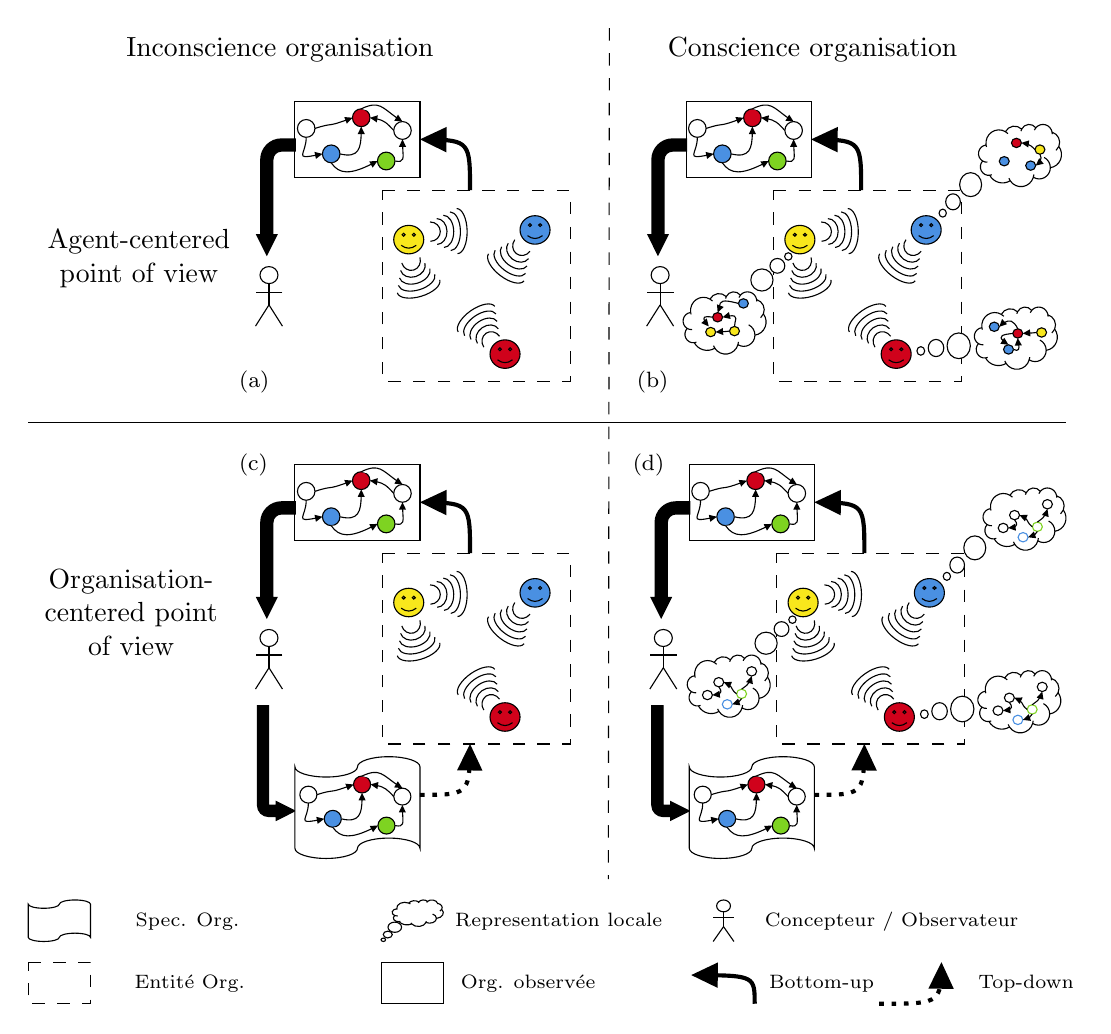
\begin{tikzpicture}[x=0.75pt,y=0.75pt,yscale=-1,xscale=1]
%uncomment if require: \path (0,1661); %set diagram left start at 0, and has height of 1661

%Shape: Cloud [id:dp19528938797470152] 
\draw  [fill={rgb, 255:red, 255; green, 255; blue, 255 }  ,fill opacity=1 ] (331.14,331.88) .. controls (330.82,329.46) and (331.88,327.06) .. (333.86,325.71) .. controls (335.85,324.36) and (338.42,324.28) .. (340.48,325.51) .. controls (341.21,324.11) and (342.55,323.14) .. (344.09,322.89) .. controls (345.63,322.65) and (347.19,323.17) .. (348.3,324.29) .. controls (348.92,323.01) and (350.14,322.15) .. (351.53,322.02) .. controls (352.92,321.88) and (354.28,322.49) .. (355.12,323.62) .. controls (356.24,322.27) and (358.03,321.7) .. (359.71,322.16) .. controls (361.39,322.62) and (362.66,324.03) .. (362.97,325.77) .. controls (364.34,326.16) and (365.49,327.13) .. (366.11,328.45) .. controls (366.73,329.76) and (366.77,331.29) .. (366.2,332.63) .. controls (367.56,334.44) and (367.88,336.84) .. (367.04,338.95) .. controls (366.2,341.05) and (364.33,342.55) .. (362.12,342.87) .. controls (362.11,344.84) and (361.05,346.66) .. (359.35,347.61) .. controls (357.65,348.56) and (355.58,348.5) .. (353.94,347.46) .. controls (353.24,349.82) and (351.27,351.57) .. (348.88,351.93) .. controls (346.49,352.29) and (344.12,351.21) .. (342.77,349.16) .. controls (341.13,350.17) and (339.15,350.46) .. (337.3,349.97) .. controls (335.44,349.47) and (333.86,348.23) .. (332.9,346.52) .. controls (331.22,346.72) and (329.6,345.84) .. (328.83,344.3) .. controls (328.07,342.76) and (328.33,340.9) .. (329.49,339.64) .. controls (327.99,338.73) and (327.22,336.95) .. (327.59,335.2) .. controls (327.96,333.46) and (329.38,332.15) .. (331.11,331.97) ; \draw   (329.49,339.64) .. controls (330.2,340.06) and (331.01,340.26) .. (331.83,340.19)(332.9,346.52) .. controls (333.25,346.48) and (333.6,346.39) .. (333.93,346.26)(342.77,349.16) .. controls (342.53,348.78) and (342.32,348.37) .. (342.16,347.95)(353.94,347.46) .. controls (354.07,347.03) and (354.15,346.58) .. (354.19,346.13)(362.12,342.87) .. controls (362.14,340.76) and (360.97,338.84) .. (359.11,337.91)(366.2,332.63) .. controls (365.9,333.35) and (365.44,333.99) .. (364.86,334.49)(362.97,325.77) .. controls (363.02,326.06) and (363.04,326.36) .. (363.04,326.65)(355.12,323.62) .. controls (354.84,323.96) and (354.61,324.34) .. (354.43,324.74)(348.3,324.29) .. controls (348.15,324.59) and (348.04,324.91) .. (347.97,325.25)(340.48,325.51) .. controls (340.92,325.77) and (341.32,326.09) .. (341.69,326.45)(331.14,331.88) .. controls (331.18,332.21) and (331.25,332.54) .. (331.35,332.86) ;
%Shape: Ellipse [id:dp20045654522113487] 
\draw   (356.15,329.85) .. controls (356.15,328.6) and (357.22,327.59) .. (358.55,327.59) .. controls (359.88,327.59) and (360.95,328.6) .. (360.95,329.85) .. controls (360.95,331.09) and (359.88,332.1) .. (358.55,332.1) .. controls (357.22,332.1) and (356.15,331.09) .. (356.15,329.85) -- cycle ;
%Shape: Ellipse [id:dp5160356195220477] 
\draw  [color={rgb, 255:red, 126; green, 211; blue, 33 }  ,draw opacity=1 ] (351.29,340.7) .. controls (351.29,339.45) and (352.36,338.45) .. (353.69,338.45) .. controls (355.02,338.45) and (356.1,339.45) .. (356.1,340.7) .. controls (356.1,341.94) and (355.02,342.95) .. (353.69,342.95) .. controls (352.36,342.95) and (351.29,341.94) .. (351.29,340.7) -- cycle ;
%Shape: Ellipse [id:dp2409525564375865] 
\draw  [color={rgb, 255:red, 74; green, 144; blue, 226 }  ,draw opacity=1 ] (344.4,345.74) .. controls (344.4,344.49) and (345.47,343.48) .. (346.8,343.48) .. controls (348.13,343.48) and (349.2,344.49) .. (349.2,345.74) .. controls (349.2,346.98) and (348.13,347.99) .. (346.8,347.99) .. controls (345.47,347.99) and (344.4,346.98) .. (344.4,345.74) -- cycle ;
%Curve Lines [id:da5915338019174681] 
\draw [fill={rgb, 255:red, 255; green, 255; blue, 255 }  ,fill opacity=1 ]   (351.29,340.7) .. controls (348.44,338.54) and (349.58,337.79) .. (347.74,336.47) ;
\draw [shift={(345.11,335.08)}, rotate = 23.5] [fill={rgb, 255:red, 0; green, 0; blue, 0 }  ][line width=0.08]  [draw opacity=0] (3.57,-1.72) -- (0,0) -- (3.57,1.72) -- cycle    ;
%Shape: Ellipse [id:dp7650379431870593] 
\draw   (340.3,335.08) .. controls (340.3,333.83) and (341.37,332.83) .. (342.7,332.83) .. controls (344.03,332.83) and (345.11,333.83) .. (345.11,335.08) .. controls (345.11,336.32) and (344.03,337.33) .. (342.7,337.33) .. controls (341.37,337.33) and (340.3,336.32) .. (340.3,335.08) -- cycle ;
%Curve Lines [id:da9568062574948017] 
\draw [fill={rgb, 255:red, 255; green, 255; blue, 255 }  ,fill opacity=1 ]   (353.69,338.45) .. controls (354.79,337.22) and (356.13,337.32) .. (357.44,334.87) ;
\draw [shift={(358.55,332.1)}, rotate = 107.08] [fill={rgb, 255:red, 0; green, 0; blue, 0 }  ][line width=0.08]  [draw opacity=0] (3.57,-1.72) -- (0,0) -- (3.57,1.72) -- cycle    ;
%Shape: Ellipse [id:dp9945538983225337] 
\draw   (334.83,341.27) .. controls (334.83,340.02) and (335.91,339.02) .. (337.24,339.02) .. controls (338.56,339.02) and (339.64,340.02) .. (339.64,341.27) .. controls (339.64,342.51) and (338.56,343.52) .. (337.24,343.52) .. controls (335.91,343.52) and (334.83,342.51) .. (334.83,341.27) -- cycle ;
%Curve Lines [id:da5828153636997717] 
\draw [fill={rgb, 255:red, 255; green, 255; blue, 255 }  ,fill opacity=1 ]   (353.69,342.95) .. controls (352.67,344.19) and (352.35,344.67) .. (352.07,344.89) ;
\draw [shift={(349.2,345.74)}, rotate = 341.19] [fill={rgb, 255:red, 0; green, 0; blue, 0 }  ][line width=0.08]  [draw opacity=0] (3.57,-1.72) -- (0,0) -- (3.57,1.72) -- cycle    ;
%Curve Lines [id:da7758791060336989] 
\draw [fill={rgb, 255:red, 255; green, 255; blue, 255 }  ,fill opacity=1 ]   (342.7,337.33) .. controls (344.34,339.32) and (343.82,340.25) .. (342.55,340.73) ;
\draw [shift={(339.64,341.27)}, rotate = 353.99] [fill={rgb, 255:red, 0; green, 0; blue, 0 }  ][line width=0.08]  [draw opacity=0] (3.57,-1.72) -- (0,0) -- (3.57,1.72) -- cycle    ;

%Shape: Cloud [id:dp6757171810574312] 
\draw  [fill={rgb, 255:red, 255; green, 255; blue, 255 }  ,fill opacity=1 ] (471.14,339.38) .. controls (470.82,336.96) and (471.88,334.56) .. (473.86,333.21) .. controls (475.85,331.86) and (478.42,331.78) .. (480.48,333.01) .. controls (481.21,331.61) and (482.55,330.64) .. (484.09,330.39) .. controls (485.63,330.15) and (487.19,330.67) .. (488.3,331.79) .. controls (488.92,330.51) and (490.14,329.65) .. (491.53,329.52) .. controls (492.92,329.38) and (494.28,329.99) .. (495.12,331.12) .. controls (496.24,329.77) and (498.03,329.2) .. (499.71,329.66) .. controls (501.39,330.12) and (502.66,331.53) .. (502.97,333.27) .. controls (504.34,333.66) and (505.49,334.63) .. (506.11,335.95) .. controls (506.73,337.26) and (506.77,338.79) .. (506.2,340.13) .. controls (507.56,341.94) and (507.88,344.34) .. (507.04,346.45) .. controls (506.2,348.55) and (504.33,350.05) .. (502.12,350.37) .. controls (502.11,352.34) and (501.05,354.16) .. (499.35,355.11) .. controls (497.65,356.06) and (495.58,356) .. (493.94,354.96) .. controls (493.24,357.32) and (491.27,359.07) .. (488.88,359.43) .. controls (486.49,359.79) and (484.12,358.71) .. (482.77,356.66) .. controls (481.13,357.67) and (479.15,357.96) .. (477.3,357.47) .. controls (475.44,356.97) and (473.86,355.73) .. (472.9,354.02) .. controls (471.22,354.22) and (469.6,353.34) .. (468.83,351.8) .. controls (468.07,350.26) and (468.33,348.4) .. (469.49,347.14) .. controls (467.99,346.23) and (467.22,344.45) .. (467.59,342.7) .. controls (467.96,340.96) and (469.38,339.65) .. (471.11,339.47) ; \draw   (469.49,347.14) .. controls (470.2,347.56) and (471.01,347.76) .. (471.83,347.69)(472.9,354.02) .. controls (473.25,353.98) and (473.6,353.89) .. (473.93,353.76)(482.77,356.66) .. controls (482.53,356.28) and (482.32,355.87) .. (482.16,355.45)(493.94,354.96) .. controls (494.07,354.53) and (494.15,354.08) .. (494.19,353.63)(502.12,350.37) .. controls (502.14,348.26) and (500.97,346.34) .. (499.11,345.41)(506.2,340.13) .. controls (505.9,340.85) and (505.44,341.49) .. (504.86,341.99)(502.97,333.27) .. controls (503.02,333.56) and (503.04,333.86) .. (503.04,334.15)(495.12,331.12) .. controls (494.84,331.46) and (494.61,331.84) .. (494.43,332.24)(488.3,331.79) .. controls (488.15,332.09) and (488.04,332.41) .. (487.97,332.75)(480.48,333.01) .. controls (480.92,333.27) and (481.32,333.59) .. (481.69,333.95)(471.14,339.38) .. controls (471.18,339.71) and (471.25,340.04) .. (471.35,340.36) ;
%Shape: Ellipse [id:dp36740066632393154] 
\draw   (496.15,337.35) .. controls (496.15,336.1) and (497.22,335.09) .. (498.55,335.09) .. controls (499.88,335.09) and (500.95,336.1) .. (500.95,337.35) .. controls (500.95,338.59) and (499.88,339.6) .. (498.55,339.6) .. controls (497.22,339.6) and (496.15,338.59) .. (496.15,337.35) -- cycle ;
%Shape: Ellipse [id:dp6735996448101857] 
\draw  [color={rgb, 255:red, 126; green, 211; blue, 33 }  ,draw opacity=1 ] (491.29,348.2) .. controls (491.29,346.95) and (492.36,345.95) .. (493.69,345.95) .. controls (495.02,345.95) and (496.1,346.95) .. (496.1,348.2) .. controls (496.1,349.44) and (495.02,350.45) .. (493.69,350.45) .. controls (492.36,350.45) and (491.29,349.44) .. (491.29,348.2) -- cycle ;
%Shape: Ellipse [id:dp9057422977098057] 
\draw  [color={rgb, 255:red, 74; green, 144; blue, 226 }  ,draw opacity=1 ] (484.4,353.24) .. controls (484.4,351.99) and (485.47,350.98) .. (486.8,350.98) .. controls (488.13,350.98) and (489.2,351.99) .. (489.2,353.24) .. controls (489.2,354.48) and (488.13,355.49) .. (486.8,355.49) .. controls (485.47,355.49) and (484.4,354.48) .. (484.4,353.24) -- cycle ;
%Curve Lines [id:da995081389821721] 
\draw [fill={rgb, 255:red, 255; green, 255; blue, 255 }  ,fill opacity=1 ]   (491.29,348.2) .. controls (488.44,346.04) and (489.58,345.29) .. (487.74,343.97) ;
\draw [shift={(485.11,342.58)}, rotate = 23.5] [fill={rgb, 255:red, 0; green, 0; blue, 0 }  ][line width=0.08]  [draw opacity=0] (3.57,-1.72) -- (0,0) -- (3.57,1.72) -- cycle    ;
%Shape: Ellipse [id:dp511750531559336] 
\draw   (480.3,342.58) .. controls (480.3,341.33) and (481.37,340.33) .. (482.7,340.33) .. controls (484.03,340.33) and (485.11,341.33) .. (485.11,342.58) .. controls (485.11,343.82) and (484.03,344.83) .. (482.7,344.83) .. controls (481.37,344.83) and (480.3,343.82) .. (480.3,342.58) -- cycle ;
%Curve Lines [id:da21484163927436972] 
\draw [fill={rgb, 255:red, 255; green, 255; blue, 255 }  ,fill opacity=1 ]   (493.69,345.95) .. controls (494.79,344.72) and (496.13,344.82) .. (497.44,342.37) ;
\draw [shift={(498.55,339.6)}, rotate = 107.08] [fill={rgb, 255:red, 0; green, 0; blue, 0 }  ][line width=0.08]  [draw opacity=0] (3.57,-1.72) -- (0,0) -- (3.57,1.72) -- cycle    ;
%Shape: Ellipse [id:dp581602588817042] 
\draw   (474.83,348.77) .. controls (474.83,347.52) and (475.91,346.52) .. (477.24,346.52) .. controls (478.56,346.52) and (479.64,347.52) .. (479.64,348.77) .. controls (479.64,350.01) and (478.56,351.02) .. (477.24,351.02) .. controls (475.91,351.02) and (474.83,350.01) .. (474.83,348.77) -- cycle ;
%Curve Lines [id:da7386901523107792] 
\draw [fill={rgb, 255:red, 255; green, 255; blue, 255 }  ,fill opacity=1 ]   (493.69,350.45) .. controls (492.67,351.69) and (492.35,352.17) .. (492.07,352.39) ;
\draw [shift={(489.2,353.24)}, rotate = 341.19] [fill={rgb, 255:red, 0; green, 0; blue, 0 }  ][line width=0.08]  [draw opacity=0] (3.57,-1.72) -- (0,0) -- (3.57,1.72) -- cycle    ;
%Curve Lines [id:da1616182330305993] 
\draw [fill={rgb, 255:red, 255; green, 255; blue, 255 }  ,fill opacity=1 ]   (482.7,344.83) .. controls (484.34,346.82) and (483.82,347.75) .. (482.55,348.23) ;
\draw [shift={(479.64,348.77)}, rotate = 353.99] [fill={rgb, 255:red, 0; green, 0; blue, 0 }  ][line width=0.08]  [draw opacity=0] (3.57,-1.72) -- (0,0) -- (3.57,1.72) -- cycle    ;

%Shape: Cloud [id:dp24886198761594924] 
\draw  [fill={rgb, 255:red, 255; green, 255; blue, 255 }  ,fill opacity=1 ] (473.64,251.38) .. controls (473.32,248.96) and (474.38,246.56) .. (476.36,245.21) .. controls (478.35,243.86) and (480.92,243.78) .. (482.98,245.01) .. controls (483.71,243.61) and (485.05,242.64) .. (486.59,242.39) .. controls (488.13,242.15) and (489.69,242.67) .. (490.8,243.79) .. controls (491.42,242.51) and (492.64,241.65) .. (494.03,241.52) .. controls (495.42,241.38) and (496.78,241.99) .. (497.62,243.12) .. controls (498.74,241.77) and (500.53,241.2) .. (502.21,241.66) .. controls (503.89,242.12) and (505.16,243.53) .. (505.47,245.27) .. controls (506.84,245.66) and (507.99,246.63) .. (508.61,247.95) .. controls (509.23,249.26) and (509.27,250.79) .. (508.7,252.13) .. controls (510.06,253.94) and (510.38,256.34) .. (509.54,258.45) .. controls (508.7,260.55) and (506.83,262.05) .. (504.62,262.37) .. controls (504.61,264.34) and (503.55,266.16) .. (501.85,267.11) .. controls (500.15,268.06) and (498.08,268) .. (496.44,266.96) .. controls (495.74,269.32) and (493.77,271.07) .. (491.38,271.43) .. controls (488.99,271.79) and (486.62,270.71) .. (485.27,268.66) .. controls (483.63,269.67) and (481.65,269.96) .. (479.8,269.47) .. controls (477.94,268.97) and (476.36,267.73) .. (475.4,266.02) .. controls (473.72,266.22) and (472.1,265.34) .. (471.33,263.8) .. controls (470.57,262.26) and (470.83,260.4) .. (471.99,259.14) .. controls (470.49,258.23) and (469.72,256.45) .. (470.09,254.7) .. controls (470.46,252.96) and (471.88,251.65) .. (473.61,251.47) ; \draw   (471.99,259.14) .. controls (472.7,259.56) and (473.51,259.76) .. (474.33,259.69)(475.4,266.02) .. controls (475.75,265.98) and (476.1,265.89) .. (476.43,265.76)(485.27,268.66) .. controls (485.03,268.28) and (484.82,267.87) .. (484.66,267.45)(496.44,266.96) .. controls (496.57,266.53) and (496.65,266.08) .. (496.69,265.63)(504.62,262.37) .. controls (504.64,260.26) and (503.47,258.34) .. (501.61,257.41)(508.7,252.13) .. controls (508.4,252.85) and (507.94,253.49) .. (507.36,253.99)(505.47,245.27) .. controls (505.52,245.56) and (505.54,245.86) .. (505.54,246.15)(497.62,243.12) .. controls (497.34,243.46) and (497.11,243.84) .. (496.93,244.24)(490.8,243.79) .. controls (490.65,244.09) and (490.54,244.41) .. (490.47,244.75)(482.98,245.01) .. controls (483.42,245.27) and (483.82,245.59) .. (484.19,245.95)(473.64,251.38) .. controls (473.68,251.71) and (473.75,252.04) .. (473.85,252.36) ;
%Shape: Ellipse [id:dp3714195505543674] 
\draw   (498.65,249.35) .. controls (498.65,248.1) and (499.72,247.09) .. (501.05,247.09) .. controls (502.38,247.09) and (503.45,248.1) .. (503.45,249.35) .. controls (503.45,250.59) and (502.38,251.6) .. (501.05,251.6) .. controls (499.72,251.6) and (498.65,250.59) .. (498.65,249.35) -- cycle ;
%Shape: Ellipse [id:dp6433500964532655] 
\draw  [color={rgb, 255:red, 126; green, 211; blue, 33 }  ,draw opacity=1 ] (493.79,260.2) .. controls (493.79,258.95) and (494.86,257.95) .. (496.19,257.95) .. controls (497.52,257.95) and (498.6,258.95) .. (498.6,260.2) .. controls (498.6,261.44) and (497.52,262.45) .. (496.19,262.45) .. controls (494.86,262.45) and (493.79,261.44) .. (493.79,260.2) -- cycle ;
%Shape: Ellipse [id:dp2637409829243822] 
\draw  [color={rgb, 255:red, 74; green, 144; blue, 226 }  ,draw opacity=1 ] (486.9,265.24) .. controls (486.9,263.99) and (487.97,262.98) .. (489.3,262.98) .. controls (490.63,262.98) and (491.7,263.99) .. (491.7,265.24) .. controls (491.7,266.48) and (490.63,267.49) .. (489.3,267.49) .. controls (487.97,267.49) and (486.9,266.48) .. (486.9,265.24) -- cycle ;
%Curve Lines [id:da5631188708920092] 
\draw [fill={rgb, 255:red, 255; green, 255; blue, 255 }  ,fill opacity=1 ]   (493.79,260.2) .. controls (490.94,258.04) and (492.08,257.29) .. (490.24,255.97) ;
\draw [shift={(487.61,254.58)}, rotate = 23.5] [fill={rgb, 255:red, 0; green, 0; blue, 0 }  ][line width=0.08]  [draw opacity=0] (3.57,-1.72) -- (0,0) -- (3.57,1.72) -- cycle    ;
%Shape: Ellipse [id:dp8107214105094749] 
\draw   (482.8,254.58) .. controls (482.8,253.33) and (483.87,252.33) .. (485.2,252.33) .. controls (486.53,252.33) and (487.61,253.33) .. (487.61,254.58) .. controls (487.61,255.82) and (486.53,256.83) .. (485.2,256.83) .. controls (483.87,256.83) and (482.8,255.82) .. (482.8,254.58) -- cycle ;
%Curve Lines [id:da6793909009127135] 
\draw [fill={rgb, 255:red, 255; green, 255; blue, 255 }  ,fill opacity=1 ]   (496.19,257.95) .. controls (497.29,256.72) and (498.63,256.82) .. (499.94,254.37) ;
\draw [shift={(501.05,251.6)}, rotate = 107.08] [fill={rgb, 255:red, 0; green, 0; blue, 0 }  ][line width=0.08]  [draw opacity=0] (3.57,-1.72) -- (0,0) -- (3.57,1.72) -- cycle    ;
%Shape: Ellipse [id:dp21056560776274869] 
\draw   (477.33,260.77) .. controls (477.33,259.52) and (478.41,258.52) .. (479.74,258.52) .. controls (481.06,258.52) and (482.14,259.52) .. (482.14,260.77) .. controls (482.14,262.01) and (481.06,263.02) .. (479.74,263.02) .. controls (478.41,263.02) and (477.33,262.01) .. (477.33,260.77) -- cycle ;
%Curve Lines [id:da016616298023254705] 
\draw [fill={rgb, 255:red, 255; green, 255; blue, 255 }  ,fill opacity=1 ]   (496.19,262.45) .. controls (495.17,263.69) and (494.85,264.17) .. (494.57,264.39) ;
\draw [shift={(491.7,265.24)}, rotate = 341.19] [fill={rgb, 255:red, 0; green, 0; blue, 0 }  ][line width=0.08]  [draw opacity=0] (3.57,-1.72) -- (0,0) -- (3.57,1.72) -- cycle    ;
%Curve Lines [id:da3006283628396156] 
\draw [fill={rgb, 255:red, 255; green, 255; blue, 255 }  ,fill opacity=1 ]   (485.2,256.83) .. controls (486.84,258.82) and (486.32,259.75) .. (485.05,260.23) ;
\draw [shift={(482.14,260.77)}, rotate = 353.99] [fill={rgb, 255:red, 0; green, 0; blue, 0 }  ][line width=0.08]  [draw opacity=0] (3.57,-1.72) -- (0,0) -- (3.57,1.72) -- cycle    ;

%Straight Lines [id:da9600905266262915] 
\draw    (10,210) -- (510,210) ;
%Straight Lines [id:da8545000281170149] 
\draw  [dash pattern={on 4.5pt off 4.5pt}]  (290,20) -- (289.5,430) ;
%Shape: Rectangle [id:dp10703839639017065] 
\draw  [dash pattern={on 4.5pt off 4.5pt}] (370.68,272.9) -- (461.05,272.9) -- (461.05,364.84) -- (370.68,364.84) -- cycle ;
%Shape: Smiley Face [id:dp3869479243277134] 
\draw  [fill={rgb, 255:red, 248; green, 231; blue, 28 }  ,fill opacity=1 ] (376.1,296.68) .. controls (376.1,292.89) and (379.34,289.82) .. (383.33,289.82) .. controls (387.32,289.82) and (390.56,292.89) .. (390.56,296.68) .. controls (390.56,300.48) and (387.32,303.55) .. (383.33,303.55) .. controls (379.34,303.55) and (376.1,300.48) .. (376.1,296.68) -- cycle ; \draw  [fill={rgb, 255:red, 248; green, 231; blue, 28 }  ,fill opacity=1 ] (380.15,294.35) .. controls (380.15,293.97) and (380.47,293.66) .. (380.87,293.66) .. controls (381.27,293.66) and (381.59,293.97) .. (381.59,294.35) .. controls (381.59,294.73) and (381.27,295.04) .. (380.87,295.04) .. controls (380.47,295.04) and (380.15,294.73) .. (380.15,294.35) -- cycle ; \draw  [fill={rgb, 255:red, 248; green, 231; blue, 28 }  ,fill opacity=1 ] (385.06,294.35) .. controls (385.06,293.97) and (385.39,293.66) .. (385.79,293.66) .. controls (386.19,293.66) and (386.51,293.97) .. (386.51,294.35) .. controls (386.51,294.73) and (386.19,295.04) .. (385.79,295.04) .. controls (385.39,295.04) and (385.06,294.73) .. (385.06,294.35) -- cycle ; \draw   (379.71,299.43) .. controls (382.12,301.26) and (384.53,301.26) .. (386.94,299.43) ;
%Shape: Arc [id:dp8237609377452255] 
\draw  [draw opacity=0] (398.28,316.11) .. controls (399.05,318.72) and (395.09,322.23) .. (389.44,323.95) .. controls (383.78,325.67) and (378.58,324.94) .. (377.81,322.33) -- (388.05,319.22) -- cycle ; \draw   (398.28,316.11) .. controls (399.05,318.72) and (395.09,322.23) .. (389.44,323.95) .. controls (383.78,325.67) and (378.58,324.94) .. (377.81,322.33) ;  
%Shape: Arc [id:dp5232395763928064] 
\draw  [draw opacity=0] (395.89,313.4) .. controls (395.89,313.4) and (395.89,313.4) .. (395.89,313.4) .. controls (395.89,313.4) and (395.89,313.4) .. (395.89,313.4) .. controls (396.66,316.01) and (393.36,319.32) .. (388.51,320.8) .. controls (383.67,322.27) and (379.12,321.35) .. (378.35,318.74) -- (387.12,316.07) -- cycle ; \draw   (395.89,313.4) .. controls (395.89,313.4) and (395.89,313.4) .. (395.89,313.4) .. controls (395.89,313.4) and (395.89,313.4) .. (395.89,313.4) .. controls (396.66,316.01) and (393.36,319.32) .. (388.51,320.8) .. controls (383.67,322.27) and (379.12,321.35) .. (378.35,318.74) ;  
%Shape: Arc [id:dp3907996654045398] 
\draw  [draw opacity=0] (393.51,310.7) .. controls (393.51,310.7) and (393.51,310.7) .. (393.51,310.7) .. controls (394.27,313.31) and (391.62,316.42) .. (387.58,317.65) .. controls (383.55,318.87) and (379.65,317.75) .. (378.89,315.14) -- (386.2,312.92) -- cycle ; \draw   (393.51,310.7) .. controls (393.51,310.7) and (393.51,310.7) .. (393.51,310.7) .. controls (394.27,313.31) and (391.62,316.42) .. (387.58,317.65) .. controls (383.55,318.87) and (379.65,317.75) .. (378.89,315.14) ;  
%Shape: Arc [id:dp6774300693433266] 
\draw  [draw opacity=0] (391.12,307.99) .. controls (391.12,307.99) and (391.12,307.99) .. (391.12,307.99) .. controls (391.12,307.99) and (391.12,307.99) .. (391.12,307.99) .. controls (391.89,310.6) and (389.89,313.51) .. (386.66,314.49) .. controls (383.43,315.48) and (380.19,314.16) .. (379.42,311.55) -- (385.27,309.77) -- cycle ; \draw   (391.12,307.99) .. controls (391.12,307.99) and (391.12,307.99) .. (391.12,307.99) .. controls (391.12,307.99) and (391.12,307.99) .. (391.12,307.99) .. controls (391.89,310.6) and (389.89,313.51) .. (386.66,314.49) .. controls (383.43,315.48) and (380.19,314.16) .. (379.42,311.55) ;  
%Shape: Arc [id:dp5904986105414511] 
\draw  [draw opacity=0] (388.73,305.28) .. controls (388.73,305.28) and (388.73,305.28) .. (388.73,305.28) .. controls (389.5,307.89) and (388.16,310.61) .. (385.73,311.34) .. controls (383.31,312.08) and (380.73,310.56) .. (379.96,307.95) -- (384.34,306.62) -- cycle ; \draw   (388.73,305.28) .. controls (388.73,305.28) and (388.73,305.28) .. (388.73,305.28) .. controls (389.5,307.89) and (388.16,310.61) .. (385.73,311.34) .. controls (383.31,312.08) and (380.73,310.56) .. (379.96,307.95) ;  

%Shape: Arc [id:dp5943283724296453] 
\draw  [draw opacity=0] (406.41,281.72) .. controls (406.41,281.72) and (406.41,281.72) .. (406.41,281.72) .. controls (409.08,281.67) and (411.35,286.49) .. (411.46,292.49) .. controls (411.58,298.49) and (409.5,303.4) .. (406.83,303.45) -- (406.62,292.59) -- cycle ; \draw   (406.41,281.72) .. controls (406.41,281.72) and (406.41,281.72) .. (406.41,281.72) .. controls (409.08,281.67) and (411.35,286.49) .. (411.46,292.49) .. controls (411.58,298.49) and (409.5,303.4) .. (406.83,303.45) ;  
%Shape: Arc [id:dp7408810368893224] 
\draw  [draw opacity=0] (403.2,283.34) .. controls (405.88,283.28) and (408.13,287.41) .. (408.23,292.55) .. controls (408.33,297.7) and (406.24,301.91) .. (403.57,301.96) -- (403.38,292.65) -- cycle ; \draw   (403.2,283.34) .. controls (405.88,283.28) and (408.13,287.41) .. (408.23,292.55) .. controls (408.33,297.7) and (406.24,301.91) .. (403.57,301.96) ;  
%Shape: Arc [id:dp8224484878672862] 
\draw  [draw opacity=0] (400,284.95) .. controls (400,284.95) and (400,284.95) .. (400,284.95) .. controls (402.68,284.9) and (404.92,288.33) .. (405,292.62) .. controls (405.08,296.9) and (402.98,300.42) .. (400.3,300.48) -- (400.15,292.72) -- cycle ; \draw   (400,284.95) .. controls (400,284.95) and (400,284.95) .. (400,284.95) .. controls (402.68,284.9) and (404.92,288.33) .. (405,292.62) .. controls (405.08,296.9) and (402.98,300.42) .. (400.3,300.48) ;  
%Shape: Arc [id:dp36884512812877546] 
\draw  [draw opacity=0] (396.8,286.57) .. controls (396.8,286.57) and (396.8,286.57) .. (396.8,286.57) .. controls (399.48,286.52) and (401.7,289.25) .. (401.77,292.68) .. controls (401.84,296.11) and (399.72,298.94) .. (397.04,298.99) .. controls (397.04,298.99) and (397.04,298.99) .. (397.04,298.99) -- (396.92,292.78) -- cycle ; \draw   (396.8,286.57) .. controls (396.8,286.57) and (396.8,286.57) .. (396.8,286.57) .. controls (399.48,286.52) and (401.7,289.25) .. (401.77,292.68) .. controls (401.84,296.11) and (399.72,298.94) .. (397.04,298.99) .. controls (397.04,298.99) and (397.04,298.99) .. (397.04,298.99) ;  
%Shape: Arc [id:dp3915492188453855] 
\draw  [draw opacity=0] (393.6,288.19) .. controls (393.6,288.19) and (393.6,288.19) .. (393.6,288.19) .. controls (396.28,288.13) and (398.49,290.18) .. (398.54,292.75) .. controls (398.59,295.32) and (396.46,297.45) .. (393.78,297.5) -- (393.69,292.85) -- cycle ; \draw   (393.6,288.19) .. controls (393.6,288.19) and (393.6,288.19) .. (393.6,288.19) .. controls (396.28,288.13) and (398.49,290.18) .. (398.54,292.75) .. controls (398.59,295.32) and (396.46,297.45) .. (393.78,297.5) ;  

%Shape: Smiley Face [id:dp988614598957863] 
\draw  [fill={rgb, 255:red, 208; green, 2; blue, 27 }  ,fill opacity=1 ] (422.49,351.85) .. controls (422.49,348.05) and (425.72,344.98) .. (429.72,344.98) .. controls (433.71,344.98) and (436.95,348.05) .. (436.95,351.85) .. controls (436.95,355.64) and (433.71,358.71) .. (429.72,358.71) .. controls (425.72,358.71) and (422.49,355.64) .. (422.49,351.85) -- cycle ; \draw  [fill={rgb, 255:red, 208; green, 2; blue, 27 }  ,fill opacity=1 ] (426.54,349.51) .. controls (426.54,349.13) and (426.86,348.82) .. (427.26,348.82) .. controls (427.66,348.82) and (427.98,349.13) .. (427.98,349.51) .. controls (427.98,349.89) and (427.66,350.2) .. (427.26,350.2) .. controls (426.86,350.2) and (426.54,349.89) .. (426.54,349.51) -- cycle ; \draw  [fill={rgb, 255:red, 208; green, 2; blue, 27 }  ,fill opacity=1 ] (431.45,349.51) .. controls (431.45,349.13) and (431.78,348.82) .. (432.18,348.82) .. controls (432.57,348.82) and (432.9,349.13) .. (432.9,349.51) .. controls (432.9,349.89) and (432.57,350.2) .. (432.18,350.2) .. controls (431.78,350.2) and (431.45,349.89) .. (431.45,349.51) -- cycle ; \draw   (426.1,354.59) .. controls (428.51,356.42) and (430.92,356.42) .. (433.33,354.59) ;
%Shape: Arc [id:dp8753083142807865] 
\draw  [draw opacity=0] (407.16,341.18) .. controls (405.64,338.93) and (408.36,334.36) .. (413.22,330.96) .. controls (418.09,327.57) and (423.26,326.64) .. (424.78,328.88) -- (415.97,335.03) -- cycle ; \draw   (407.16,341.18) .. controls (405.64,338.93) and (408.36,334.36) .. (413.22,330.96) .. controls (418.09,327.57) and (423.26,326.64) .. (424.78,328.88) ;  
%Shape: Arc [id:dp6777143782771846] 
\draw  [draw opacity=0] (410.24,343.01) .. controls (410.24,343.01) and (410.24,343.01) .. (410.24,343.01) .. controls (410.24,343.01) and (410.24,343.01) .. (410.24,343.01) .. controls (408.73,340.76) and (410.88,336.58) .. (415.05,333.67) .. controls (419.22,330.76) and (423.83,330.23) .. (425.35,332.47) -- (417.79,337.74) -- cycle ; \draw   (410.24,343.01) .. controls (410.24,343.01) and (410.24,343.01) .. (410.24,343.01) .. controls (410.24,343.01) and (410.24,343.01) .. (410.24,343.01) .. controls (408.73,340.76) and (410.88,336.58) .. (415.05,333.67) .. controls (419.22,330.76) and (423.83,330.23) .. (425.35,332.47) ;  
%Shape: Arc [id:dp3547186961595412] 
\draw  [draw opacity=0] (413.33,344.84) .. controls (413.33,344.84) and (413.33,344.84) .. (413.33,344.84) .. controls (411.82,342.6) and (413.41,338.81) .. (416.88,336.39) .. controls (420.36,333.96) and (424.4,333.82) .. (425.92,336.06) -- (419.62,340.45) -- cycle ; \draw   (413.33,344.84) .. controls (413.33,344.84) and (413.33,344.84) .. (413.33,344.84) .. controls (411.82,342.6) and (413.41,338.81) .. (416.88,336.39) .. controls (420.36,333.96) and (424.4,333.82) .. (425.92,336.06) ;  
%Shape: Arc [id:dp2128251501338161] 
\draw  [draw opacity=0] (416.42,346.68) .. controls (416.42,346.68) and (416.42,346.68) .. (416.42,346.68) .. controls (414.9,344.43) and (415.93,341.04) .. (418.71,339.1) .. controls (421.49,337.16) and (424.97,337.41) .. (426.49,339.65) -- (421.45,343.17) -- cycle ; \draw   (416.42,346.68) .. controls (416.42,346.68) and (416.42,346.68) .. (416.42,346.68) .. controls (414.9,344.43) and (415.93,341.04) .. (418.71,339.1) .. controls (421.49,337.16) and (424.97,337.41) .. (426.49,339.65) ;  
%Shape: Arc [id:dp5571107725474194] 
\draw  [draw opacity=0] (419.5,348.51) .. controls (417.99,346.27) and (418.45,343.26) .. (420.54,341.81) .. controls (422.62,340.36) and (425.54,341) .. (427.05,343.24) -- (423.28,345.88) -- cycle ; \draw   (419.5,348.51) .. controls (417.99,346.27) and (418.45,343.26) .. (420.54,341.81) .. controls (422.62,340.36) and (425.54,341) .. (427.05,343.24) ;  

%Shape: Smiley Face [id:dp9623754418294168] 
\draw  [fill={rgb, 255:red, 74; green, 144; blue, 226 }  ,fill opacity=1 ] (436.95,292.03) .. controls (436.95,288.23) and (440.18,285.16) .. (444.18,285.16) .. controls (448.17,285.16) and (451.41,288.23) .. (451.41,292.03) .. controls (451.41,295.82) and (448.17,298.89) .. (444.18,298.89) .. controls (440.18,298.89) and (436.95,295.82) .. (436.95,292.03) -- cycle ; \draw  [fill={rgb, 255:red, 74; green, 144; blue, 226 }  ,fill opacity=1 ] (441,289.69) .. controls (441,289.31) and (441.32,289.01) .. (441.72,289.01) .. controls (442.12,289.01) and (442.44,289.31) .. (442.44,289.69) .. controls (442.44,290.07) and (442.12,290.38) .. (441.72,290.38) .. controls (441.32,290.38) and (441,290.07) .. (441,289.69) -- cycle ; \draw  [fill={rgb, 255:red, 74; green, 144; blue, 226 }  ,fill opacity=1 ] (445.91,289.69) .. controls (445.91,289.31) and (446.24,289.01) .. (446.63,289.01) .. controls (447.03,289.01) and (447.36,289.31) .. (447.36,289.69) .. controls (447.36,290.07) and (447.03,290.38) .. (446.63,290.38) .. controls (446.24,290.38) and (445.91,290.07) .. (445.91,289.69) -- cycle ; \draw   (440.56,294.77) .. controls (442.97,296.6) and (445.38,296.6) .. (447.79,294.77) ;
%Shape: Arc [id:dp7665865548370878] 
\draw  [draw opacity=0] (438.88,316.55) .. controls (438.88,316.55) and (438.88,316.55) .. (438.88,316.55) .. controls (437.27,318.72) and (432.14,317.57) .. (427.42,313.98) .. controls (422.7,310.38) and (420.18,305.69) .. (421.78,303.51) -- (430.33,310.03) -- cycle ; \draw   (438.88,316.55) .. controls (438.88,316.55) and (438.88,316.55) .. (438.88,316.55) .. controls (437.27,318.72) and (432.14,317.57) .. (427.42,313.98) .. controls (422.7,310.38) and (420.18,305.69) .. (421.78,303.51) ;  
%Shape: Arc [id:dp6649623287433064] 
\draw  [draw opacity=0] (439.6,312.98) .. controls (437.99,315.16) and (433.41,314.43) .. (429.36,311.34) .. controls (425.31,308.26) and (423.34,303.99) .. (424.94,301.81) -- (432.27,307.4) -- cycle ; \draw   (439.6,312.98) .. controls (437.99,315.16) and (433.41,314.43) .. (429.36,311.34) .. controls (425.31,308.26) and (423.34,303.99) .. (424.94,301.81) ;  
%Shape: Arc [id:dp7430892960379802] 
\draw  [draw opacity=0] (440.31,309.42) .. controls (440.31,309.42) and (440.31,309.42) .. (440.31,309.42) .. controls (438.71,311.6) and (434.67,311.28) .. (431.3,308.71) .. controls (427.93,306.14) and (426.49,302.29) .. (428.1,300.11) -- (434.21,304.77) -- cycle ; \draw   (440.31,309.42) .. controls (440.31,309.42) and (440.31,309.42) .. (440.31,309.42) .. controls (438.71,311.6) and (434.67,311.28) .. (431.3,308.71) .. controls (427.93,306.14) and (426.49,302.29) .. (428.1,300.11) ;  
%Shape: Arc [id:dp3945653964835283] 
\draw  [draw opacity=0] (441.03,305.86) .. controls (441.03,305.86) and (441.03,305.86) .. (441.03,305.86) .. controls (439.42,308.04) and (435.94,308.14) .. (433.24,306.08) .. controls (430.54,304.02) and (429.65,300.59) .. (431.26,298.41) -- (436.15,302.13) -- cycle ; \draw   (441.03,305.86) .. controls (441.03,305.86) and (441.03,305.86) .. (441.03,305.86) .. controls (439.42,308.04) and (435.94,308.14) .. (433.24,306.08) .. controls (430.54,304.02) and (429.65,300.59) .. (431.26,298.41) ;  
%Shape: Arc [id:dp42497989160292815] 
\draw  [draw opacity=0] (441.75,302.29) .. controls (440.14,304.47) and (437.2,304.99) .. (435.18,303.45) .. controls (433.15,301.91) and (432.81,298.89) .. (434.42,296.71) -- (438.08,299.5) -- cycle ; \draw   (441.75,302.29) .. controls (440.14,304.47) and (437.2,304.99) .. (435.18,303.45) .. controls (433.15,301.91) and (432.81,298.89) .. (434.42,296.71) ;  

%Shape: Rectangle [id:dp546857417644991] 
\draw  [fill={rgb, 255:red, 255; green, 255; blue, 255 }  ,fill opacity=1 ] (328.5,230) -- (388.75,230) -- (388.75,266.77) -- (328.5,266.77) -- cycle ;
%Shape: Ellipse [id:dp24918374283361144] 
\draw  [fill={rgb, 255:red, 255; green, 255; blue, 255 }  ,fill opacity=1 ] (329.71,243.12) .. controls (329.71,240.75) and (331.6,238.83) .. (333.93,238.83) .. controls (336.26,238.83) and (338.14,240.75) .. (338.14,243.12) .. controls (338.14,245.49) and (336.26,247.41) .. (333.93,247.41) .. controls (331.6,247.41) and (329.71,245.49) .. (329.71,243.12) -- cycle ;
%Shape: Ellipse [id:dp5450965462940762] 
\draw  [fill={rgb, 255:red, 74; green, 144; blue, 226 }  ,fill opacity=1 ] (341.76,255.37) .. controls (341.76,253) and (343.65,251.08) .. (345.98,251.08) .. controls (348.31,251.08) and (350.19,253) .. (350.19,255.37) .. controls (350.19,257.74) and (348.31,259.66) .. (345.98,259.66) .. controls (343.65,259.66) and (341.76,257.74) .. (341.76,255.37) -- cycle ;
%Shape: Ellipse [id:dp7987375819279374] 
\draw  [fill={rgb, 255:red, 208; green, 2; blue, 27 }  ,fill opacity=1 ] (356.22,237.97) .. controls (356.22,235.6) and (358.11,233.68) .. (360.44,233.68) .. controls (362.76,233.68) and (364.65,235.6) .. (364.65,237.97) .. controls (364.65,240.34) and (362.76,242.26) .. (360.44,242.26) .. controls (358.11,242.26) and (356.22,240.34) .. (356.22,237.97) -- cycle ;
%Shape: Ellipse [id:dp5534074056729055] 
\draw  [fill={rgb, 255:red, 255; green, 255; blue, 255 }  ,fill opacity=1 ] (376.1,244.1) .. controls (376.1,241.73) and (377.99,239.81) .. (380.32,239.81) .. controls (382.65,239.81) and (384.53,241.73) .. (384.53,244.1) .. controls (384.53,246.47) and (382.65,248.39) .. (380.32,248.39) .. controls (377.99,248.39) and (376.1,246.47) .. (376.1,244.1) -- cycle ;
%Shape: Ellipse [id:dp16861920570326183] 
\draw  [fill={rgb, 255:red, 126; green, 211; blue, 33 }  ,fill opacity=1 ] (368.27,258.81) .. controls (368.27,256.44) and (370.16,254.52) .. (372.48,254.52) .. controls (374.81,254.52) and (376.7,256.44) .. (376.7,258.81) .. controls (376.7,261.18) and (374.81,263.1) .. (372.48,263.1) .. controls (370.16,263.1) and (368.27,261.18) .. (368.27,258.81) -- cycle ;
%Curve Lines [id:da39315316180596604] 
\draw [fill={rgb, 255:red, 255; green, 255; blue, 255 }  ,fill opacity=1 ]   (338.14,243.12) .. controls (347.62,240.05) and (343.17,242.76) .. (353.42,239.01) ;
\draw [shift={(356.22,237.97)}, rotate = 159.17] [fill={rgb, 255:red, 0; green, 0; blue, 0 }  ][line width=0.08]  [draw opacity=0] (3.57,-1.72) -- (0,0) -- (3.57,1.72) -- cycle    ;
%Curve Lines [id:da4175483162604987] 
\draw [fill={rgb, 255:red, 255; green, 255; blue, 255 }  ,fill opacity=1 ]   (350.19,255.37) .. controls (359.26,257.65) and (360.3,252.63) .. (360.42,245.25) ;
\draw [shift={(360.44,242.26)}, rotate = 90] [fill={rgb, 255:red, 0; green, 0; blue, 0 }  ][line width=0.08]  [draw opacity=0] (3.57,-1.72) -- (0,0) -- (3.57,1.72) -- cycle    ;
%Curve Lines [id:da42460565406359896] 
\draw [fill={rgb, 255:red, 255; green, 255; blue, 255 }  ,fill opacity=1 ]   (376.1,244.1) .. controls (372.6,240.33) and (371.59,239.27) .. (367.56,238.46) ;
\draw [shift={(364.65,237.97)}, rotate = 8.42] [fill={rgb, 255:red, 0; green, 0; blue, 0 }  ][line width=0.08]  [draw opacity=0] (3.57,-1.72) -- (0,0) -- (3.57,1.72) -- cycle    ;
%Curve Lines [id:da015834809446955367] 
\draw [fill={rgb, 255:red, 255; green, 255; blue, 255 }  ,fill opacity=1 ]   (376.7,258.81) .. controls (381.47,259.67) and (380.65,257.87) .. (380.38,251.33) ;
\draw [shift={(380.32,248.39)}, rotate = 90] [fill={rgb, 255:red, 0; green, 0; blue, 0 }  ][line width=0.08]  [draw opacity=0] (3.57,-1.72) -- (0,0) -- (3.57,1.72) -- cycle    ;
%Curve Lines [id:da09383707527505059] 
\draw [fill={rgb, 255:red, 255; green, 255; blue, 255 }  ,fill opacity=1 ]   (333.93,247.41) .. controls (333.93,255.5) and (327.67,258.19) .. (338.91,255.96) ;
\draw [shift={(341.76,255.37)}, rotate = 168.05] [fill={rgb, 255:red, 0; green, 0; blue, 0 }  ][line width=0.08]  [draw opacity=0] (3.57,-1.72) -- (0,0) -- (3.57,1.72) -- cycle    ;
%Curve Lines [id:da23718287082828216] 
\draw [fill={rgb, 255:red, 255; green, 255; blue, 255 }  ,fill opacity=1 ]   (345.98,259.66) .. controls (349.88,265.45) and (355.32,265.36) .. (365.66,260.17) ;
\draw [shift={(368.27,258.81)}, rotate = 151.67] [fill={rgb, 255:red, 0; green, 0; blue, 0 }  ][line width=0.08]  [draw opacity=0] (3.57,-1.72) -- (0,0) -- (3.57,1.72) -- cycle    ;
%Curve Lines [id:da28563814500050566] 
\draw [fill={rgb, 255:red, 255; green, 255; blue, 255 }  ,fill opacity=1 ]   (360.44,233.68) .. controls (369.21,229.44) and (370.5,233.12) .. (377.92,238.25) ;
\draw [shift={(380.32,239.81)}, rotate = 211.4] [fill={rgb, 255:red, 0; green, 0; blue, 0 }  ][line width=0.08]  [draw opacity=0] (3.57,-1.72) -- (0,0) -- (3.57,1.72) -- cycle    ;
%Bend Arrow [id:dp14494363252865816] 
\draw  [fill={rgb, 255:red, 0; green, 0; blue, 0 }  ,fill opacity=1 ] (310.43,346.45) -- (310.43,394.38) .. controls (310.43,397.38) and (312.86,399.81) .. (315.85,399.81) -- (319.47,399.81) -- (319.47,401.61) -- (328.5,397.09) -- (319.47,392.58) -- (319.47,394.38) -- (315.85,394.38) .. controls (315.85,394.38) and (315.85,394.38) .. (315.85,394.38) -- (315.85,346.45) -- cycle ;
%Shape: Ellipse [id:dp34407288704185013] 
\draw   (311.66,313.78) .. controls (311.66,311.51) and (313.6,309.68) .. (315.99,309.68) .. controls (318.38,309.68) and (320.32,311.51) .. (320.32,313.78) .. controls (320.32,316.04) and (318.38,317.88) .. (315.99,317.88) .. controls (313.6,317.88) and (311.66,316.04) .. (311.66,313.78) -- cycle ;
%Straight Lines [id:da960872603126619] 
\draw    (315.99,317.88) -- (315.99,328.12) ;
%Straight Lines [id:da02863617740959179] 
\draw    (315.99,328.12) -- (309.5,338.37) ;
%Straight Lines [id:da09592937404823143] 
\draw    (315.99,328.12) -- (322.48,338.37) ;
%Straight Lines [id:da3956257675851418] 
\draw    (322.48,321.98) -- (309.5,321.98) ;

%Bend Arrow [id:dp7504124150412457] 
\draw  [fill={rgb, 255:red, 0; green, 0; blue, 0 }  ,fill opacity=1 ][line width=0.75]  (328.5,248.39) -- (322,248.39) .. controls (316.61,248.39) and (312.24,252.76) .. (312.24,258.15) -- (312.24,294.51) -- (310.43,294.51) -- (314.95,303.55) -- (319.47,294.51) -- (317.66,294.51) -- (317.66,258.15) .. controls (317.66,255.75) and (319.6,253.81) .. (322,253.81) -- (328.5,253.81) -- cycle ;
%Flowchart: Punched Tape [id:dp9872594248314814] 
\draw  [fill={rgb, 255:red, 255; green, 255; blue, 255 }  ,fill opacity=1 ] (328.5,375.87) .. controls (328.5,378.58) and (335.25,380.77) .. (343.57,380.77) .. controls (351.88,380.77) and (358.63,378.58) .. (358.63,375.87) .. controls (358.63,373.16) and (365.37,370.97) .. (373.69,370.97) .. controls (382.01,370.97) and (388.75,373.16) .. (388.75,375.87) -- (388.75,415.1) .. controls (388.75,412.39) and (382.01,410.19) .. (373.69,410.19) .. controls (365.37,410.19) and (358.63,412.39) .. (358.63,415.1) .. controls (358.63,417.8) and (351.88,420) .. (343.57,420) .. controls (335.25,420) and (328.5,417.8) .. (328.5,415.1) -- cycle ;
%Shape: Ellipse [id:dp9937474442416085] 
\draw  [fill={rgb, 255:red, 255; green, 255; blue, 255 }  ,fill opacity=1 ] (330.86,389.26) .. controls (330.86,387.01) and (332.7,385.18) .. (334.97,385.18) .. controls (337.25,385.18) and (339.09,387.01) .. (339.09,389.26) .. controls (339.09,391.51) and (337.25,393.33) .. (334.97,393.33) .. controls (332.7,393.33) and (330.86,391.51) .. (330.86,389.26) -- cycle ;
%Shape: Ellipse [id:dp696973406112954] 
\draw  [fill={rgb, 255:red, 74; green, 144; blue, 226 }  ,fill opacity=1 ] (342.62,400.91) .. controls (342.62,398.65) and (344.46,396.83) .. (346.73,396.83) .. controls (349.01,396.83) and (350.85,398.65) .. (350.85,400.91) .. controls (350.85,403.16) and (349.01,404.98) .. (346.73,404.98) .. controls (344.46,404.98) and (342.62,403.16) .. (342.62,400.91) -- cycle ;
%Shape: Ellipse [id:dp6539295815985688] 
\draw  [fill={rgb, 255:red, 208; green, 2; blue, 27 }  ,fill opacity=1 ] (356.73,384.36) .. controls (356.73,382.11) and (358.57,380.29) .. (360.85,380.29) .. controls (363.12,380.29) and (364.96,382.11) .. (364.96,384.36) .. controls (364.96,386.62) and (363.12,388.44) .. (360.85,388.44) .. controls (358.57,388.44) and (356.73,386.62) .. (356.73,384.36) -- cycle ;
%Shape: Ellipse [id:dp633915390476385] 
\draw  [fill={rgb, 255:red, 255; green, 255; blue, 255 }  ,fill opacity=1 ] (376.13,390.19) .. controls (376.13,387.94) and (377.98,386.11) .. (380.25,386.11) .. controls (382.52,386.11) and (384.37,387.94) .. (384.37,390.19) .. controls (384.37,392.44) and (382.52,394.27) .. (380.25,394.27) .. controls (377.98,394.27) and (376.13,392.44) .. (376.13,390.19) -- cycle ;
%Shape: Ellipse [id:dp6416083133951336] 
\draw  [fill={rgb, 255:red, 126; green, 211; blue, 33 }  ,fill opacity=1 ] (368.49,404.17) .. controls (368.49,401.92) and (370.33,400.09) .. (372.61,400.09) .. controls (374.88,400.09) and (376.72,401.92) .. (376.72,404.17) .. controls (376.72,406.42) and (374.88,408.24) .. (372.61,408.24) .. controls (370.33,408.24) and (368.49,406.42) .. (368.49,404.17) -- cycle ;
%Curve Lines [id:da6276833595037365] 
\draw [fill={rgb, 255:red, 255; green, 255; blue, 255 }  ,fill opacity=1 ]   (339.09,389.26) .. controls (348.34,386.35) and (344,388.92) .. (354,385.36) ;
\draw [shift={(356.73,384.36)}, rotate = 159.68] [fill={rgb, 255:red, 0; green, 0; blue, 0 }  ][line width=0.08]  [draw opacity=0] (3.57,-1.72) -- (0,0) -- (3.57,1.72) -- cycle    ;
%Curve Lines [id:da06674481461522297] 
\draw [fill={rgb, 255:red, 255; green, 255; blue, 255 }  ,fill opacity=1 ]   (350.85,400.91) .. controls (359.65,403.06) and (360.7,398.36) .. (360.83,391.4) ;
\draw [shift={(360.85,388.44)}, rotate = 90] [fill={rgb, 255:red, 0; green, 0; blue, 0 }  ][line width=0.08]  [draw opacity=0] (3.57,-1.72) -- (0,0) -- (3.57,1.72) -- cycle    ;
%Curve Lines [id:da7021701347418892] 
\draw [fill={rgb, 255:red, 255; green, 255; blue, 255 }  ,fill opacity=1 ]   (376.13,390.19) .. controls (372.74,386.63) and (371.74,385.61) .. (367.87,384.84) ;
\draw [shift={(364.96,384.36)}, rotate = 8.2] [fill={rgb, 255:red, 0; green, 0; blue, 0 }  ][line width=0.08]  [draw opacity=0] (3.57,-1.72) -- (0,0) -- (3.57,1.72) -- cycle    ;
%Curve Lines [id:da22084028756933338] 
\draw [fill={rgb, 255:red, 255; green, 255; blue, 255 }  ,fill opacity=1 ]   (376.72,404.17) .. controls (381.35,404.98) and (380.58,403.3) .. (380.32,397.17) ;
\draw [shift={(380.25,394.27)}, rotate = 90] [fill={rgb, 255:red, 0; green, 0; blue, 0 }  ][line width=0.08]  [draw opacity=0] (3.57,-1.72) -- (0,0) -- (3.57,1.72) -- cycle    ;
%Curve Lines [id:da713039546157396] 
\draw [fill={rgb, 255:red, 255; green, 255; blue, 255 }  ,fill opacity=1 ]   (334.97,393.33) .. controls (334.97,401.03) and (328.87,403.58) .. (339.84,401.46) ;
\draw [shift={(342.62,400.91)}, rotate = 168.36] [fill={rgb, 255:red, 0; green, 0; blue, 0 }  ][line width=0.08]  [draw opacity=0] (3.57,-1.72) -- (0,0) -- (3.57,1.72) -- cycle    ;
%Curve Lines [id:da5097502528215505] 
\draw [fill={rgb, 255:red, 255; green, 255; blue, 255 }  ,fill opacity=1 ]   (346.73,404.98) .. controls (350.54,410.48) and (355.86,410.39) .. (365.94,405.46) ;
\draw [shift={(368.49,404.17)}, rotate = 152.3] [fill={rgb, 255:red, 0; green, 0; blue, 0 }  ][line width=0.08]  [draw opacity=0] (3.57,-1.72) -- (0,0) -- (3.57,1.72) -- cycle    ;
%Curve Lines [id:da542437045911365] 
\draw [fill={rgb, 255:red, 255; green, 255; blue, 255 }  ,fill opacity=1 ]   (360.85,380.29) .. controls (369.36,376.28) and (370.65,379.72) .. (377.79,384.55) ;
\draw [shift={(380.25,386.11)}, rotate = 210.72] [fill={rgb, 255:red, 0; green, 0; blue, 0 }  ][line width=0.08]  [draw opacity=0] (3.57,-1.72) -- (0,0) -- (3.57,1.72) -- cycle    ;
%Curve Lines [id:da5848843590813868] 
\draw [line width=1.5]  [dash pattern={on 1.69pt off 2.76pt}]  (388.75,389.35) .. controls (411.3,389.35) and (412.54,389.35) .. (412.81,368.67) ;
\draw [shift={(412.85,364.84)}, rotate = 90.56] [fill={rgb, 255:red, 0; green, 0; blue, 0 }  ][line width=0.08]  [draw opacity=0] (12.77,-6.13) -- (0,0) -- (12.77,6.13) -- cycle    ;
%Shape: Boxed Bezier Curve [id:dp9234142242986265] 
\draw [line width=1.5]    (412.85,272.9) .. controls (412.85,249.97) and (412.85,248.71) .. (392.51,248.43) ;
\draw [shift={(388.75,248.39)}, rotate = 0.58] [fill={rgb, 255:red, 0; green, 0; blue, 0 }  ][line width=0.08]  [draw opacity=0] (12.77,-6.13) -- (0,0) -- (12.77,6.13) -- cycle    ;

%Shape: Rectangle [id:dp038417671609133786] 
\draw  [dash pattern={on 4.5pt off 4.5pt}] (180.68,272.9) -- (271.05,272.9) -- (271.05,364.84) -- (180.68,364.84) -- cycle ;
%Shape: Smiley Face [id:dp9716572095259455] 
\draw  [fill={rgb, 255:red, 248; green, 231; blue, 28 }  ,fill opacity=1 ] (186.1,296.68) .. controls (186.1,292.89) and (189.34,289.82) .. (193.33,289.82) .. controls (197.32,289.82) and (200.56,292.89) .. (200.56,296.68) .. controls (200.56,300.48) and (197.32,303.55) .. (193.33,303.55) .. controls (189.34,303.55) and (186.1,300.48) .. (186.1,296.68) -- cycle ; \draw  [fill={rgb, 255:red, 248; green, 231; blue, 28 }  ,fill opacity=1 ] (190.15,294.35) .. controls (190.15,293.97) and (190.47,293.66) .. (190.87,293.66) .. controls (191.27,293.66) and (191.59,293.97) .. (191.59,294.35) .. controls (191.59,294.73) and (191.27,295.04) .. (190.87,295.04) .. controls (190.47,295.04) and (190.15,294.73) .. (190.15,294.35) -- cycle ; \draw  [fill={rgb, 255:red, 248; green, 231; blue, 28 }  ,fill opacity=1 ] (195.06,294.35) .. controls (195.06,293.97) and (195.39,293.66) .. (195.79,293.66) .. controls (196.19,293.66) and (196.51,293.97) .. (196.51,294.35) .. controls (196.51,294.73) and (196.19,295.04) .. (195.79,295.04) .. controls (195.39,295.04) and (195.06,294.73) .. (195.06,294.35) -- cycle ; \draw   (189.71,299.43) .. controls (192.12,301.26) and (194.53,301.26) .. (196.94,299.43) ;
%Shape: Arc [id:dp3069489593189756] 
\draw  [draw opacity=0] (208.28,316.11) .. controls (208.28,316.11) and (208.28,316.11) .. (208.28,316.11) .. controls (209.05,318.72) and (205.09,322.23) .. (199.44,323.95) .. controls (193.78,325.67) and (188.58,324.94) .. (187.81,322.33) -- (198.05,319.22) -- cycle ; \draw   (208.28,316.11) .. controls (208.28,316.11) and (208.28,316.11) .. (208.28,316.11) .. controls (209.05,318.72) and (205.09,322.23) .. (199.44,323.95) .. controls (193.78,325.67) and (188.58,324.94) .. (187.81,322.33) ;  
%Shape: Arc [id:dp1587851862141385] 
\draw  [draw opacity=0] (205.89,313.4) .. controls (205.89,313.4) and (205.89,313.4) .. (205.89,313.4) .. controls (205.89,313.4) and (205.89,313.4) .. (205.89,313.4) .. controls (206.66,316.01) and (203.36,319.32) .. (198.51,320.8) .. controls (193.67,322.27) and (189.12,321.35) .. (188.35,318.74) -- (197.12,316.07) -- cycle ; \draw   (205.89,313.4) .. controls (205.89,313.4) and (205.89,313.4) .. (205.89,313.4) .. controls (205.89,313.4) and (205.89,313.4) .. (205.89,313.4) .. controls (206.66,316.01) and (203.36,319.32) .. (198.51,320.8) .. controls (193.67,322.27) and (189.12,321.35) .. (188.35,318.74) ;  
%Shape: Arc [id:dp3091994715315485] 
\draw  [draw opacity=0] (203.51,310.7) .. controls (203.51,310.7) and (203.51,310.7) .. (203.51,310.7) .. controls (204.27,313.31) and (201.62,316.42) .. (197.58,317.65) .. controls (193.55,318.87) and (189.65,317.75) .. (188.89,315.14) -- (196.2,312.92) -- cycle ; \draw   (203.51,310.7) .. controls (203.51,310.7) and (203.51,310.7) .. (203.51,310.7) .. controls (204.27,313.31) and (201.62,316.42) .. (197.58,317.65) .. controls (193.55,318.87) and (189.65,317.75) .. (188.89,315.14) ;  
%Shape: Arc [id:dp701724508845611] 
\draw  [draw opacity=0] (201.12,307.99) .. controls (201.12,307.99) and (201.12,307.99) .. (201.12,307.99) .. controls (201.12,307.99) and (201.12,307.99) .. (201.12,307.99) .. controls (201.89,310.6) and (199.89,313.51) .. (196.66,314.49) .. controls (193.43,315.48) and (190.19,314.16) .. (189.42,311.55) -- (195.27,309.77) -- cycle ; \draw   (201.12,307.99) .. controls (201.12,307.99) and (201.12,307.99) .. (201.12,307.99) .. controls (201.12,307.99) and (201.12,307.99) .. (201.12,307.99) .. controls (201.89,310.6) and (199.89,313.51) .. (196.66,314.49) .. controls (193.43,315.48) and (190.19,314.16) .. (189.42,311.55) ;  
%Shape: Arc [id:dp4139611225011828] 
\draw  [draw opacity=0] (198.73,305.28) .. controls (198.73,305.28) and (198.73,305.28) .. (198.73,305.28) .. controls (199.5,307.89) and (198.16,310.61) .. (195.73,311.34) .. controls (193.31,312.08) and (190.73,310.56) .. (189.96,307.95) -- (194.34,306.62) -- cycle ; \draw   (198.73,305.28) .. controls (198.73,305.28) and (198.73,305.28) .. (198.73,305.28) .. controls (199.5,307.89) and (198.16,310.61) .. (195.73,311.34) .. controls (193.31,312.08) and (190.73,310.56) .. (189.96,307.95) ;  

%Shape: Arc [id:dp3029809869694706] 
\draw  [draw opacity=0] (216.41,281.72) .. controls (216.41,281.72) and (216.41,281.72) .. (216.41,281.72) .. controls (219.08,281.67) and (221.35,286.49) .. (221.46,292.49) .. controls (221.58,298.49) and (219.5,303.4) .. (216.83,303.45) -- (216.62,292.59) -- cycle ; \draw   (216.41,281.72) .. controls (216.41,281.72) and (216.41,281.72) .. (216.41,281.72) .. controls (219.08,281.67) and (221.35,286.49) .. (221.46,292.49) .. controls (221.58,298.49) and (219.5,303.4) .. (216.83,303.45) ;  
%Shape: Arc [id:dp5165343689317023] 
\draw  [draw opacity=0] (213.2,283.34) .. controls (215.88,283.28) and (218.13,287.41) .. (218.23,292.55) .. controls (218.33,297.7) and (216.24,301.91) .. (213.57,301.96) -- (213.38,292.65) -- cycle ; \draw   (213.2,283.34) .. controls (215.88,283.28) and (218.13,287.41) .. (218.23,292.55) .. controls (218.33,297.7) and (216.24,301.91) .. (213.57,301.96) ;  
%Shape: Arc [id:dp9821431873250026] 
\draw  [draw opacity=0] (210,284.95) .. controls (210,284.95) and (210,284.95) .. (210,284.95) .. controls (212.68,284.9) and (214.92,288.33) .. (215,292.62) .. controls (215.08,296.9) and (212.98,300.42) .. (210.3,300.48) .. controls (210.3,300.48) and (210.3,300.48) .. (210.3,300.48) -- (210.15,292.72) -- cycle ; \draw   (210,284.95) .. controls (210,284.95) and (210,284.95) .. (210,284.95) .. controls (212.68,284.9) and (214.92,288.33) .. (215,292.62) .. controls (215.08,296.9) and (212.98,300.42) .. (210.3,300.48) .. controls (210.3,300.48) and (210.3,300.48) .. (210.3,300.48) ;  
%Shape: Arc [id:dp08775704034114207] 
\draw  [draw opacity=0] (206.8,286.57) .. controls (209.48,286.52) and (211.7,289.25) .. (211.77,292.68) .. controls (211.84,296.11) and (209.72,298.94) .. (207.04,298.99) -- (206.92,292.78) -- cycle ; \draw   (206.8,286.57) .. controls (209.48,286.52) and (211.7,289.25) .. (211.77,292.68) .. controls (211.84,296.11) and (209.72,298.94) .. (207.04,298.99) ;  
%Shape: Arc [id:dp5940065928919354] 
\draw  [draw opacity=0] (203.6,288.19) .. controls (203.6,288.19) and (203.6,288.19) .. (203.6,288.19) .. controls (206.28,288.13) and (208.49,290.18) .. (208.54,292.75) .. controls (208.59,295.32) and (206.46,297.45) .. (203.78,297.5) -- (203.69,292.85) -- cycle ; \draw   (203.6,288.19) .. controls (203.6,288.19) and (203.6,288.19) .. (203.6,288.19) .. controls (206.28,288.13) and (208.49,290.18) .. (208.54,292.75) .. controls (208.59,295.32) and (206.46,297.45) .. (203.78,297.5) ;  

%Shape: Smiley Face [id:dp04556614430760053] 
\draw  [fill={rgb, 255:red, 208; green, 2; blue, 27 }  ,fill opacity=1 ] (232.49,351.85) .. controls (232.49,348.05) and (235.72,344.98) .. (239.72,344.98) .. controls (243.71,344.98) and (246.95,348.05) .. (246.95,351.85) .. controls (246.95,355.64) and (243.71,358.71) .. (239.72,358.71) .. controls (235.72,358.71) and (232.49,355.64) .. (232.49,351.85) -- cycle ; \draw  [fill={rgb, 255:red, 208; green, 2; blue, 27 }  ,fill opacity=1 ] (236.54,349.51) .. controls (236.54,349.13) and (236.86,348.82) .. (237.26,348.82) .. controls (237.66,348.82) and (237.98,349.13) .. (237.98,349.51) .. controls (237.98,349.89) and (237.66,350.2) .. (237.26,350.2) .. controls (236.86,350.2) and (236.54,349.89) .. (236.54,349.51) -- cycle ; \draw  [fill={rgb, 255:red, 208; green, 2; blue, 27 }  ,fill opacity=1 ] (241.45,349.51) .. controls (241.45,349.13) and (241.78,348.82) .. (242.18,348.82) .. controls (242.57,348.82) and (242.9,349.13) .. (242.9,349.51) .. controls (242.9,349.89) and (242.57,350.2) .. (242.18,350.2) .. controls (241.78,350.2) and (241.45,349.89) .. (241.45,349.51) -- cycle ; \draw   (236.1,354.59) .. controls (238.51,356.42) and (240.92,356.42) .. (243.33,354.59) ;
%Shape: Arc [id:dp323262092827896] 
\draw  [draw opacity=0] (217.16,341.18) .. controls (217.16,341.18) and (217.16,341.18) .. (217.16,341.18) .. controls (215.64,338.93) and (218.36,334.36) .. (223.22,330.96) .. controls (228.09,327.57) and (233.26,326.64) .. (234.78,328.88) -- (225.97,335.03) -- cycle ; \draw   (217.16,341.18) .. controls (217.16,341.18) and (217.16,341.18) .. (217.16,341.18) .. controls (215.64,338.93) and (218.36,334.36) .. (223.22,330.96) .. controls (228.09,327.57) and (233.26,326.64) .. (234.78,328.88) ;  
%Shape: Arc [id:dp5974482786950237] 
\draw  [draw opacity=0] (220.24,343.01) .. controls (220.24,343.01) and (220.24,343.01) .. (220.24,343.01) .. controls (218.73,340.76) and (220.88,336.58) .. (225.05,333.67) .. controls (229.22,330.76) and (233.83,330.23) .. (235.35,332.47) -- (227.79,337.74) -- cycle ; \draw   (220.24,343.01) .. controls (220.24,343.01) and (220.24,343.01) .. (220.24,343.01) .. controls (218.73,340.76) and (220.88,336.58) .. (225.05,333.67) .. controls (229.22,330.76) and (233.83,330.23) .. (235.35,332.47) ;  
%Shape: Arc [id:dp6456518692321449] 
\draw  [draw opacity=0] (223.33,344.84) .. controls (221.82,342.6) and (223.41,338.81) .. (226.88,336.39) .. controls (230.36,333.96) and (234.4,333.82) .. (235.92,336.06) -- (229.62,340.45) -- cycle ; \draw   (223.33,344.84) .. controls (221.82,342.6) and (223.41,338.81) .. (226.88,336.39) .. controls (230.36,333.96) and (234.4,333.82) .. (235.92,336.06) ;  
%Shape: Arc [id:dp9900103513107401] 
\draw  [draw opacity=0] (226.42,346.68) .. controls (226.42,346.68) and (226.42,346.68) .. (226.42,346.68) .. controls (224.9,344.43) and (225.93,341.04) .. (228.71,339.1) .. controls (231.49,337.16) and (234.97,337.41) .. (236.49,339.65) -- (231.45,343.17) -- cycle ; \draw   (226.42,346.68) .. controls (226.42,346.68) and (226.42,346.68) .. (226.42,346.68) .. controls (224.9,344.43) and (225.93,341.04) .. (228.71,339.1) .. controls (231.49,337.16) and (234.97,337.41) .. (236.49,339.65) ;  
%Shape: Arc [id:dp6495647423177111] 
\draw  [draw opacity=0] (229.5,348.51) .. controls (229.5,348.51) and (229.5,348.51) .. (229.5,348.51) .. controls (227.99,346.27) and (228.45,343.26) .. (230.54,341.81) .. controls (232.62,340.36) and (235.54,341) .. (237.05,343.24) -- (233.28,345.88) -- cycle ; \draw   (229.5,348.51) .. controls (229.5,348.51) and (229.5,348.51) .. (229.5,348.51) .. controls (227.99,346.27) and (228.45,343.26) .. (230.54,341.81) .. controls (232.62,340.36) and (235.54,341) .. (237.05,343.24) ;  

%Shape: Smiley Face [id:dp6662307911150986] 
\draw  [fill={rgb, 255:red, 74; green, 144; blue, 226 }  ,fill opacity=1 ] (246.95,292.03) .. controls (246.95,288.23) and (250.18,285.16) .. (254.18,285.16) .. controls (258.17,285.16) and (261.41,288.23) .. (261.41,292.03) .. controls (261.41,295.82) and (258.17,298.89) .. (254.18,298.89) .. controls (250.18,298.89) and (246.95,295.82) .. (246.95,292.03) -- cycle ; \draw  [fill={rgb, 255:red, 74; green, 144; blue, 226 }  ,fill opacity=1 ] (251,289.69) .. controls (251,289.31) and (251.32,289.01) .. (251.72,289.01) .. controls (252.12,289.01) and (252.44,289.31) .. (252.44,289.69) .. controls (252.44,290.07) and (252.12,290.38) .. (251.72,290.38) .. controls (251.32,290.38) and (251,290.07) .. (251,289.69) -- cycle ; \draw  [fill={rgb, 255:red, 74; green, 144; blue, 226 }  ,fill opacity=1 ] (255.91,289.69) .. controls (255.91,289.31) and (256.24,289.01) .. (256.63,289.01) .. controls (257.03,289.01) and (257.36,289.31) .. (257.36,289.69) .. controls (257.36,290.07) and (257.03,290.38) .. (256.63,290.38) .. controls (256.24,290.38) and (255.91,290.07) .. (255.91,289.69) -- cycle ; \draw   (250.56,294.77) .. controls (252.97,296.6) and (255.38,296.6) .. (257.79,294.77) ;
%Shape: Arc [id:dp5199114206161695] 
\draw  [draw opacity=0] (248.88,316.55) .. controls (248.88,316.55) and (248.88,316.55) .. (248.88,316.55) .. controls (247.27,318.72) and (242.14,317.57) .. (237.42,313.98) .. controls (232.7,310.38) and (230.18,305.69) .. (231.78,303.51) -- (240.33,310.03) -- cycle ; \draw   (248.88,316.55) .. controls (248.88,316.55) and (248.88,316.55) .. (248.88,316.55) .. controls (247.27,318.72) and (242.14,317.57) .. (237.42,313.98) .. controls (232.7,310.38) and (230.18,305.69) .. (231.78,303.51) ;  
%Shape: Arc [id:dp9677219722001149] 
\draw  [draw opacity=0] (249.6,312.98) .. controls (249.6,312.98) and (249.6,312.98) .. (249.6,312.98) .. controls (249.6,312.98) and (249.6,312.98) .. (249.6,312.98) .. controls (247.99,315.16) and (243.41,314.43) .. (239.36,311.34) .. controls (235.31,308.26) and (233.34,303.99) .. (234.94,301.81) -- (242.27,307.4) -- cycle ; \draw   (249.6,312.98) .. controls (249.6,312.98) and (249.6,312.98) .. (249.6,312.98) .. controls (249.6,312.98) and (249.6,312.98) .. (249.6,312.98) .. controls (247.99,315.16) and (243.41,314.43) .. (239.36,311.34) .. controls (235.31,308.26) and (233.34,303.99) .. (234.94,301.81) ;  
%Shape: Arc [id:dp39029670567481345] 
\draw  [draw opacity=0] (250.31,309.42) .. controls (248.71,311.6) and (244.67,311.28) .. (241.3,308.71) .. controls (237.93,306.14) and (236.49,302.29) .. (238.1,300.11) -- (244.21,304.77) -- cycle ; \draw   (250.31,309.42) .. controls (248.71,311.6) and (244.67,311.28) .. (241.3,308.71) .. controls (237.93,306.14) and (236.49,302.29) .. (238.1,300.11) ;  
%Shape: Arc [id:dp3598307111738779] 
\draw  [draw opacity=0] (251.03,305.86) .. controls (249.42,308.04) and (245.94,308.14) .. (243.24,306.08) .. controls (240.54,304.02) and (239.65,300.59) .. (241.26,298.41) -- (246.15,302.13) -- cycle ; \draw   (251.03,305.86) .. controls (249.42,308.04) and (245.94,308.14) .. (243.24,306.08) .. controls (240.54,304.02) and (239.65,300.59) .. (241.26,298.41) ;  
%Shape: Arc [id:dp9487370596092919] 
\draw  [draw opacity=0] (251.75,302.29) .. controls (250.14,304.47) and (247.2,304.99) .. (245.18,303.45) .. controls (243.15,301.91) and (242.81,298.89) .. (244.42,296.71) -- (248.08,299.5) -- cycle ; \draw   (251.75,302.29) .. controls (250.14,304.47) and (247.2,304.99) .. (245.18,303.45) .. controls (243.15,301.91) and (242.81,298.89) .. (244.42,296.71) ;  

%Shape: Rectangle [id:dp2957771657370434] 
\draw  [fill={rgb, 255:red, 255; green, 255; blue, 255 }  ,fill opacity=1 ] (138.5,230) -- (198.75,230) -- (198.75,266.77) -- (138.5,266.77) -- cycle ;
%Shape: Ellipse [id:dp20979852086273576] 
\draw  [fill={rgb, 255:red, 255; green, 255; blue, 255 }  ,fill opacity=1 ] (139.71,243.12) .. controls (139.71,240.75) and (141.6,238.83) .. (143.93,238.83) .. controls (146.26,238.83) and (148.14,240.75) .. (148.14,243.12) .. controls (148.14,245.49) and (146.26,247.41) .. (143.93,247.41) .. controls (141.6,247.41) and (139.71,245.49) .. (139.71,243.12) -- cycle ;
%Shape: Ellipse [id:dp13050810964628412] 
\draw  [fill={rgb, 255:red, 74; green, 144; blue, 226 }  ,fill opacity=1 ] (151.76,255.37) .. controls (151.76,253) and (153.65,251.08) .. (155.98,251.08) .. controls (158.31,251.08) and (160.19,253) .. (160.19,255.37) .. controls (160.19,257.74) and (158.31,259.66) .. (155.98,259.66) .. controls (153.65,259.66) and (151.76,257.74) .. (151.76,255.37) -- cycle ;
%Shape: Ellipse [id:dp6251632817276846] 
\draw  [fill={rgb, 255:red, 208; green, 2; blue, 27 }  ,fill opacity=1 ] (166.22,237.97) .. controls (166.22,235.6) and (168.11,233.68) .. (170.44,233.68) .. controls (172.76,233.68) and (174.65,235.6) .. (174.65,237.97) .. controls (174.65,240.34) and (172.76,242.26) .. (170.44,242.26) .. controls (168.11,242.26) and (166.22,240.34) .. (166.22,237.97) -- cycle ;
%Shape: Ellipse [id:dp42202042668133233] 
\draw  [fill={rgb, 255:red, 255; green, 255; blue, 255 }  ,fill opacity=1 ] (186.1,244.1) .. controls (186.1,241.73) and (187.99,239.81) .. (190.32,239.81) .. controls (192.65,239.81) and (194.53,241.73) .. (194.53,244.1) .. controls (194.53,246.47) and (192.65,248.39) .. (190.32,248.39) .. controls (187.99,248.39) and (186.1,246.47) .. (186.1,244.1) -- cycle ;
%Shape: Ellipse [id:dp7549761595533702] 
\draw  [fill={rgb, 255:red, 126; green, 211; blue, 33 }  ,fill opacity=1 ] (178.27,258.81) .. controls (178.27,256.44) and (180.16,254.52) .. (182.48,254.52) .. controls (184.81,254.52) and (186.7,256.44) .. (186.7,258.81) .. controls (186.7,261.18) and (184.81,263.1) .. (182.48,263.1) .. controls (180.16,263.1) and (178.27,261.18) .. (178.27,258.81) -- cycle ;
%Curve Lines [id:da037381844999033076] 
\draw [fill={rgb, 255:red, 255; green, 255; blue, 255 }  ,fill opacity=1 ]   (148.14,243.12) .. controls (157.62,240.05) and (153.17,242.76) .. (163.42,239.01) ;
\draw [shift={(166.22,237.97)}, rotate = 159.17] [fill={rgb, 255:red, 0; green, 0; blue, 0 }  ][line width=0.08]  [draw opacity=0] (3.57,-1.72) -- (0,0) -- (3.57,1.72) -- cycle    ;
%Curve Lines [id:da9052970628657517] 
\draw [fill={rgb, 255:red, 255; green, 255; blue, 255 }  ,fill opacity=1 ]   (160.19,255.37) .. controls (169.26,257.65) and (170.3,252.63) .. (170.42,245.25) ;
\draw [shift={(170.44,242.26)}, rotate = 90] [fill={rgb, 255:red, 0; green, 0; blue, 0 }  ][line width=0.08]  [draw opacity=0] (3.57,-1.72) -- (0,0) -- (3.57,1.72) -- cycle    ;
%Curve Lines [id:da3591981779978355] 
\draw [fill={rgb, 255:red, 255; green, 255; blue, 255 }  ,fill opacity=1 ]   (186.1,244.1) .. controls (182.6,240.33) and (181.59,239.27) .. (177.56,238.46) ;
\draw [shift={(174.65,237.97)}, rotate = 8.42] [fill={rgb, 255:red, 0; green, 0; blue, 0 }  ][line width=0.08]  [draw opacity=0] (3.57,-1.72) -- (0,0) -- (3.57,1.72) -- cycle    ;
%Curve Lines [id:da6030519187118517] 
\draw [fill={rgb, 255:red, 255; green, 255; blue, 255 }  ,fill opacity=1 ]   (186.7,258.81) .. controls (191.47,259.67) and (190.65,257.87) .. (190.38,251.33) ;
\draw [shift={(190.32,248.39)}, rotate = 90] [fill={rgb, 255:red, 0; green, 0; blue, 0 }  ][line width=0.08]  [draw opacity=0] (3.57,-1.72) -- (0,0) -- (3.57,1.72) -- cycle    ;
%Curve Lines [id:da6041218467038296] 
\draw [fill={rgb, 255:red, 255; green, 255; blue, 255 }  ,fill opacity=1 ]   (143.93,247.41) .. controls (143.93,255.5) and (137.67,258.19) .. (148.91,255.96) ;
\draw [shift={(151.76,255.37)}, rotate = 168.05] [fill={rgb, 255:red, 0; green, 0; blue, 0 }  ][line width=0.08]  [draw opacity=0] (3.57,-1.72) -- (0,0) -- (3.57,1.72) -- cycle    ;
%Curve Lines [id:da12039507836027852] 
\draw [fill={rgb, 255:red, 255; green, 255; blue, 255 }  ,fill opacity=1 ]   (155.98,259.66) .. controls (159.88,265.45) and (165.32,265.36) .. (175.66,260.17) ;
\draw [shift={(178.27,258.81)}, rotate = 151.67] [fill={rgb, 255:red, 0; green, 0; blue, 0 }  ][line width=0.08]  [draw opacity=0] (3.57,-1.72) -- (0,0) -- (3.57,1.72) -- cycle    ;
%Curve Lines [id:da6271034651364642] 
\draw [fill={rgb, 255:red, 255; green, 255; blue, 255 }  ,fill opacity=1 ]   (170.44,233.68) .. controls (179.21,229.44) and (180.5,233.12) .. (187.92,238.25) ;
\draw [shift={(190.32,239.81)}, rotate = 211.4] [fill={rgb, 255:red, 0; green, 0; blue, 0 }  ][line width=0.08]  [draw opacity=0] (3.57,-1.72) -- (0,0) -- (3.57,1.72) -- cycle    ;
%Bend Arrow [id:dp5994501296338741] 
\draw  [fill={rgb, 255:red, 0; green, 0; blue, 0 }  ,fill opacity=1 ] (120.43,346.45) -- (120.43,394.38) .. controls (120.43,397.38) and (122.86,399.81) .. (125.85,399.81) -- (129.47,399.81) -- (129.47,401.61) -- (138.5,397.09) -- (129.47,392.58) -- (129.47,394.38) -- (125.85,394.38) .. controls (125.85,394.38) and (125.85,394.38) .. (125.85,394.38) -- (125.85,346.45) -- cycle ;
%Shape: Ellipse [id:dp9483503267525337] 
\draw   (121.66,313.78) .. controls (121.66,311.51) and (123.6,309.68) .. (125.99,309.68) .. controls (128.38,309.68) and (130.32,311.51) .. (130.32,313.78) .. controls (130.32,316.04) and (128.38,317.88) .. (125.99,317.88) .. controls (123.6,317.88) and (121.66,316.04) .. (121.66,313.78) -- cycle ;
%Straight Lines [id:da1838505962582151] 
\draw    (125.99,317.88) -- (125.99,328.12) ;
%Straight Lines [id:da6092932551055767] 
\draw    (125.99,328.12) -- (119.5,338.37) ;
%Straight Lines [id:da42866812336269966] 
\draw    (125.99,328.12) -- (132.48,338.37) ;
%Straight Lines [id:da5009018734507784] 
\draw    (132.48,321.98) -- (119.5,321.98) ;

%Bend Arrow [id:dp3981398979269859] 
\draw  [fill={rgb, 255:red, 0; green, 0; blue, 0 }  ,fill opacity=1 ][line width=0.75]  (138.5,248.39) -- (132,248.39) .. controls (126.61,248.39) and (122.24,252.76) .. (122.24,258.15) -- (122.24,294.51) -- (120.43,294.51) -- (124.95,303.55) -- (129.47,294.51) -- (127.66,294.51) -- (127.66,258.15) .. controls (127.66,255.75) and (129.6,253.81) .. (132,253.81) -- (138.5,253.81) -- cycle ;
%Flowchart: Punched Tape [id:dp42006380035009316] 
\draw  [fill={rgb, 255:red, 255; green, 255; blue, 255 }  ,fill opacity=1 ] (138.5,375.87) .. controls (138.5,378.58) and (145.25,380.77) .. (153.57,380.77) .. controls (161.88,380.77) and (168.63,378.58) .. (168.63,375.87) .. controls (168.63,373.16) and (175.37,370.97) .. (183.69,370.97) .. controls (192.01,370.97) and (198.75,373.16) .. (198.75,375.87) -- (198.75,415.1) .. controls (198.75,412.39) and (192.01,410.19) .. (183.69,410.19) .. controls (175.37,410.19) and (168.63,412.39) .. (168.63,415.1) .. controls (168.63,417.8) and (161.88,420) .. (153.57,420) .. controls (145.25,420) and (138.5,417.8) .. (138.5,415.1) -- cycle ;
%Shape: Ellipse [id:dp5635059616267319] 
\draw  [fill={rgb, 255:red, 255; green, 255; blue, 255 }  ,fill opacity=1 ] (140.86,389.26) .. controls (140.86,387.01) and (142.7,385.18) .. (144.97,385.18) .. controls (147.25,385.18) and (149.09,387.01) .. (149.09,389.26) .. controls (149.09,391.51) and (147.25,393.33) .. (144.97,393.33) .. controls (142.7,393.33) and (140.86,391.51) .. (140.86,389.26) -- cycle ;
%Shape: Ellipse [id:dp7974297068658951] 
\draw  [fill={rgb, 255:red, 74; green, 144; blue, 226 }  ,fill opacity=1 ] (152.62,400.91) .. controls (152.62,398.65) and (154.46,396.83) .. (156.73,396.83) .. controls (159.01,396.83) and (160.85,398.65) .. (160.85,400.91) .. controls (160.85,403.16) and (159.01,404.98) .. (156.73,404.98) .. controls (154.46,404.98) and (152.62,403.16) .. (152.62,400.91) -- cycle ;
%Shape: Ellipse [id:dp8226180742249218] 
\draw  [fill={rgb, 255:red, 208; green, 2; blue, 27 }  ,fill opacity=1 ] (166.73,384.36) .. controls (166.73,382.11) and (168.57,380.29) .. (170.85,380.29) .. controls (173.12,380.29) and (174.96,382.11) .. (174.96,384.36) .. controls (174.96,386.62) and (173.12,388.44) .. (170.85,388.44) .. controls (168.57,388.44) and (166.73,386.62) .. (166.73,384.36) -- cycle ;
%Shape: Ellipse [id:dp5292272091758374] 
\draw  [fill={rgb, 255:red, 255; green, 255; blue, 255 }  ,fill opacity=1 ] (186.13,390.19) .. controls (186.13,387.94) and (187.98,386.11) .. (190.25,386.11) .. controls (192.52,386.11) and (194.37,387.94) .. (194.37,390.19) .. controls (194.37,392.44) and (192.52,394.27) .. (190.25,394.27) .. controls (187.98,394.27) and (186.13,392.44) .. (186.13,390.19) -- cycle ;
%Shape: Ellipse [id:dp3560245105912889] 
\draw  [fill={rgb, 255:red, 126; green, 211; blue, 33 }  ,fill opacity=1 ] (178.49,404.17) .. controls (178.49,401.92) and (180.33,400.09) .. (182.61,400.09) .. controls (184.88,400.09) and (186.72,401.92) .. (186.72,404.17) .. controls (186.72,406.42) and (184.88,408.24) .. (182.61,408.24) .. controls (180.33,408.24) and (178.49,406.42) .. (178.49,404.17) -- cycle ;
%Curve Lines [id:da6155160971922808] 
\draw [fill={rgb, 255:red, 255; green, 255; blue, 255 }  ,fill opacity=1 ]   (149.09,389.26) .. controls (158.34,386.35) and (154,388.92) .. (164,385.36) ;
\draw [shift={(166.73,384.36)}, rotate = 159.68] [fill={rgb, 255:red, 0; green, 0; blue, 0 }  ][line width=0.08]  [draw opacity=0] (3.57,-1.72) -- (0,0) -- (3.57,1.72) -- cycle    ;
%Curve Lines [id:da6781256698011275] 
\draw [fill={rgb, 255:red, 255; green, 255; blue, 255 }  ,fill opacity=1 ]   (160.85,400.91) .. controls (169.65,403.06) and (170.7,398.36) .. (170.83,391.4) ;
\draw [shift={(170.85,388.44)}, rotate = 90] [fill={rgb, 255:red, 0; green, 0; blue, 0 }  ][line width=0.08]  [draw opacity=0] (3.57,-1.72) -- (0,0) -- (3.57,1.72) -- cycle    ;
%Curve Lines [id:da47025147472172724] 
\draw [fill={rgb, 255:red, 255; green, 255; blue, 255 }  ,fill opacity=1 ]   (186.13,390.19) .. controls (182.74,386.63) and (181.74,385.61) .. (177.87,384.84) ;
\draw [shift={(174.96,384.36)}, rotate = 8.2] [fill={rgb, 255:red, 0; green, 0; blue, 0 }  ][line width=0.08]  [draw opacity=0] (3.57,-1.72) -- (0,0) -- (3.57,1.72) -- cycle    ;
%Curve Lines [id:da6625936610581984] 
\draw [fill={rgb, 255:red, 255; green, 255; blue, 255 }  ,fill opacity=1 ]   (186.72,404.17) .. controls (191.35,404.98) and (190.58,403.3) .. (190.32,397.17) ;
\draw [shift={(190.25,394.27)}, rotate = 90] [fill={rgb, 255:red, 0; green, 0; blue, 0 }  ][line width=0.08]  [draw opacity=0] (3.57,-1.72) -- (0,0) -- (3.57,1.72) -- cycle    ;
%Curve Lines [id:da5608684264163912] 
\draw [fill={rgb, 255:red, 255; green, 255; blue, 255 }  ,fill opacity=1 ]   (144.97,393.33) .. controls (144.97,401.03) and (138.87,403.58) .. (149.84,401.46) ;
\draw [shift={(152.62,400.91)}, rotate = 168.36] [fill={rgb, 255:red, 0; green, 0; blue, 0 }  ][line width=0.08]  [draw opacity=0] (3.57,-1.72) -- (0,0) -- (3.57,1.72) -- cycle    ;
%Curve Lines [id:da7743408531851985] 
\draw [fill={rgb, 255:red, 255; green, 255; blue, 255 }  ,fill opacity=1 ]   (156.73,404.98) .. controls (160.54,410.48) and (165.86,410.39) .. (175.94,405.46) ;
\draw [shift={(178.49,404.17)}, rotate = 152.3] [fill={rgb, 255:red, 0; green, 0; blue, 0 }  ][line width=0.08]  [draw opacity=0] (3.57,-1.72) -- (0,0) -- (3.57,1.72) -- cycle    ;
%Curve Lines [id:da6802699451949246] 
\draw [fill={rgb, 255:red, 255; green, 255; blue, 255 }  ,fill opacity=1 ]   (170.85,380.29) .. controls (179.36,376.28) and (180.65,379.72) .. (187.79,384.55) ;
\draw [shift={(190.25,386.11)}, rotate = 210.72] [fill={rgb, 255:red, 0; green, 0; blue, 0 }  ][line width=0.08]  [draw opacity=0] (3.57,-1.72) -- (0,0) -- (3.57,1.72) -- cycle    ;
%Curve Lines [id:da9676248578679112] 
\draw [line width=1.5]  [dash pattern={on 1.69pt off 2.76pt}]  (198.75,389.35) .. controls (221.3,389.35) and (222.54,389.35) .. (222.81,368.67) ;
\draw [shift={(222.85,364.84)}, rotate = 90.56] [fill={rgb, 255:red, 0; green, 0; blue, 0 }  ][line width=0.08]  [draw opacity=0] (12.77,-6.13) -- (0,0) -- (12.77,6.13) -- cycle    ;
%Shape: Boxed Bezier Curve [id:dp47475506369988985] 
\draw [line width=1.5]    (222.85,272.9) .. controls (222.85,249.97) and (222.85,248.71) .. (202.51,248.43) ;
\draw [shift={(198.75,248.39)}, rotate = 0.58] [fill={rgb, 255:red, 0; green, 0; blue, 0 }  ][line width=0.08]  [draw opacity=0] (12.77,-6.13) -- (0,0) -- (12.77,6.13) -- cycle    ;

%Shape: Rectangle [id:dp10985824181702597] 
\draw  [dash pattern={on 4.5pt off 4.5pt}] (180.68,98.06) -- (271.05,98.06) -- (271.05,190) -- (180.68,190) -- cycle ;
%Shape: Smiley Face [id:dp11853519791695377] 
\draw  [fill={rgb, 255:red, 248; green, 231; blue, 28 }  ,fill opacity=1 ] (186.1,121.85) .. controls (186.1,118.05) and (189.34,114.98) .. (193.33,114.98) .. controls (197.32,114.98) and (200.56,118.05) .. (200.56,121.85) .. controls (200.56,125.64) and (197.32,128.71) .. (193.33,128.71) .. controls (189.34,128.71) and (186.1,125.64) .. (186.1,121.85) -- cycle ; \draw  [fill={rgb, 255:red, 248; green, 231; blue, 28 }  ,fill opacity=1 ] (190.15,119.51) .. controls (190.15,119.13) and (190.47,118.82) .. (190.87,118.82) .. controls (191.27,118.82) and (191.59,119.13) .. (191.59,119.51) .. controls (191.59,119.89) and (191.27,120.2) .. (190.87,120.2) .. controls (190.47,120.2) and (190.15,119.89) .. (190.15,119.51) -- cycle ; \draw  [fill={rgb, 255:red, 248; green, 231; blue, 28 }  ,fill opacity=1 ] (195.06,119.51) .. controls (195.06,119.13) and (195.39,118.82) .. (195.79,118.82) .. controls (196.19,118.82) and (196.51,119.13) .. (196.51,119.51) .. controls (196.51,119.89) and (196.19,120.2) .. (195.79,120.2) .. controls (195.39,120.2) and (195.06,119.89) .. (195.06,119.51) -- cycle ; \draw   (189.71,124.59) .. controls (192.12,126.42) and (194.53,126.42) .. (196.94,124.59) ;
%Shape: Arc [id:dp6754768208026447] 
\draw  [draw opacity=0] (208.28,141.27) .. controls (208.28,141.27) and (208.28,141.27) .. (208.28,141.27) .. controls (209.05,143.88) and (205.09,147.39) .. (199.44,149.11) .. controls (193.78,150.83) and (188.58,150.1) .. (187.81,147.49) -- (198.05,144.38) -- cycle ; \draw   (208.28,141.27) .. controls (208.28,141.27) and (208.28,141.27) .. (208.28,141.27) .. controls (209.05,143.88) and (205.09,147.39) .. (199.44,149.11) .. controls (193.78,150.83) and (188.58,150.1) .. (187.81,147.49) ;  
%Shape: Arc [id:dp03482702928344561] 
\draw  [draw opacity=0] (205.89,138.56) .. controls (205.89,138.56) and (205.89,138.56) .. (205.89,138.56) .. controls (205.89,138.56) and (205.89,138.56) .. (205.89,138.56) .. controls (206.66,141.17) and (203.36,144.48) .. (198.51,145.96) .. controls (193.67,147.43) and (189.12,146.51) .. (188.35,143.9) -- (197.12,141.23) -- cycle ; \draw   (205.89,138.56) .. controls (205.89,138.56) and (205.89,138.56) .. (205.89,138.56) .. controls (205.89,138.56) and (205.89,138.56) .. (205.89,138.56) .. controls (206.66,141.17) and (203.36,144.48) .. (198.51,145.96) .. controls (193.67,147.43) and (189.12,146.51) .. (188.35,143.9) ;  
%Shape: Arc [id:dp7395691989556363] 
\draw  [draw opacity=0] (203.51,135.86) .. controls (203.51,135.86) and (203.51,135.86) .. (203.51,135.86) .. controls (204.27,138.47) and (201.62,141.58) .. (197.58,142.81) .. controls (193.55,144.03) and (189.65,142.91) .. (188.89,140.3) -- (196.2,138.08) -- cycle ; \draw   (203.51,135.86) .. controls (203.51,135.86) and (203.51,135.86) .. (203.51,135.86) .. controls (204.27,138.47) and (201.62,141.58) .. (197.58,142.81) .. controls (193.55,144.03) and (189.65,142.91) .. (188.89,140.3) ;  
%Shape: Arc [id:dp3847175649180483] 
\draw  [draw opacity=0] (201.12,133.15) .. controls (201.12,133.15) and (201.12,133.15) .. (201.12,133.15) .. controls (201.12,133.15) and (201.12,133.15) .. (201.12,133.15) .. controls (201.89,135.76) and (199.89,138.67) .. (196.66,139.66) .. controls (193.43,140.64) and (190.19,139.32) .. (189.42,136.71) -- (195.27,134.93) -- cycle ; \draw   (201.12,133.15) .. controls (201.12,133.15) and (201.12,133.15) .. (201.12,133.15) .. controls (201.12,133.15) and (201.12,133.15) .. (201.12,133.15) .. controls (201.89,135.76) and (199.89,138.67) .. (196.66,139.66) .. controls (193.43,140.64) and (190.19,139.32) .. (189.42,136.71) ;  
%Shape: Arc [id:dp6059625465577667] 
\draw  [draw opacity=0] (198.73,130.44) .. controls (198.73,130.44) and (198.73,130.44) .. (198.73,130.44) .. controls (199.5,133.05) and (198.16,135.77) .. (195.73,136.5) .. controls (193.31,137.24) and (190.73,135.72) .. (189.96,133.11) -- (194.34,131.78) -- cycle ; \draw   (198.73,130.44) .. controls (198.73,130.44) and (198.73,130.44) .. (198.73,130.44) .. controls (199.5,133.05) and (198.16,135.77) .. (195.73,136.5) .. controls (193.31,137.24) and (190.73,135.72) .. (189.96,133.11) ;  

%Shape: Arc [id:dp9185323435685564] 
\draw  [draw opacity=0] (216.41,106.88) .. controls (216.41,106.88) and (216.41,106.88) .. (216.41,106.88) .. controls (219.08,106.83) and (221.35,111.65) .. (221.46,117.65) .. controls (221.58,123.65) and (219.5,128.56) .. (216.83,128.61) -- (216.62,117.75) -- cycle ; \draw   (216.41,106.88) .. controls (216.41,106.88) and (216.41,106.88) .. (216.41,106.88) .. controls (219.08,106.83) and (221.35,111.65) .. (221.46,117.65) .. controls (221.58,123.65) and (219.5,128.56) .. (216.83,128.61) ;  
%Shape: Arc [id:dp9585350368762569] 
\draw  [draw opacity=0] (213.2,108.5) .. controls (215.88,108.44) and (218.13,112.57) .. (218.23,117.71) .. controls (218.33,122.86) and (216.24,127.07) .. (213.57,127.13) -- (213.38,117.81) -- cycle ; \draw   (213.2,108.5) .. controls (215.88,108.44) and (218.13,112.57) .. (218.23,117.71) .. controls (218.33,122.86) and (216.24,127.07) .. (213.57,127.13) ;  
%Shape: Arc [id:dp5800421881645605] 
\draw  [draw opacity=0] (210,110.12) .. controls (210,110.12) and (210,110.12) .. (210,110.12) .. controls (212.68,110.06) and (214.92,113.49) .. (215,117.78) .. controls (215.08,122.07) and (212.98,125.58) .. (210.3,125.64) .. controls (210.3,125.64) and (210.3,125.64) .. (210.3,125.64) -- (210.15,117.88) -- cycle ; \draw   (210,110.12) .. controls (210,110.12) and (210,110.12) .. (210,110.12) .. controls (212.68,110.06) and (214.92,113.49) .. (215,117.78) .. controls (215.08,122.07) and (212.98,125.58) .. (210.3,125.64) .. controls (210.3,125.64) and (210.3,125.64) .. (210.3,125.64) ;  
%Shape: Arc [id:dp5797548244988138] 
\draw  [draw opacity=0] (206.8,111.73) .. controls (209.48,111.68) and (211.7,114.42) .. (211.77,117.84) .. controls (211.84,121.27) and (209.72,124.1) .. (207.04,124.15) -- (206.92,117.94) -- cycle ; \draw   (206.8,111.73) .. controls (209.48,111.68) and (211.7,114.42) .. (211.77,117.84) .. controls (211.84,121.27) and (209.72,124.1) .. (207.04,124.15) ;  
%Shape: Arc [id:dp48509365144208627] 
\draw  [draw opacity=0] (203.6,113.35) .. controls (203.6,113.35) and (203.6,113.35) .. (203.6,113.35) .. controls (206.28,113.3) and (208.49,115.34) .. (208.54,117.91) .. controls (208.59,120.48) and (206.46,122.61) .. (203.78,122.66) -- (203.69,118.01) -- cycle ; \draw   (203.6,113.35) .. controls (203.6,113.35) and (203.6,113.35) .. (203.6,113.35) .. controls (206.28,113.3) and (208.49,115.34) .. (208.54,117.91) .. controls (208.59,120.48) and (206.46,122.61) .. (203.78,122.66) ;  

%Shape: Smiley Face [id:dp5611227831026884] 
\draw  [fill={rgb, 255:red, 208; green, 2; blue, 27 }  ,fill opacity=1 ] (232.49,177.01) .. controls (232.49,173.22) and (235.72,170.14) .. (239.72,170.14) .. controls (243.71,170.14) and (246.95,173.22) .. (246.95,177.01) .. controls (246.95,180.8) and (243.71,183.87) .. (239.72,183.87) .. controls (235.72,183.87) and (232.49,180.8) .. (232.49,177.01) -- cycle ; \draw  [fill={rgb, 255:red, 208; green, 2; blue, 27 }  ,fill opacity=1 ] (236.54,174.67) .. controls (236.54,174.29) and (236.86,173.99) .. (237.26,173.99) .. controls (237.66,173.99) and (237.98,174.29) .. (237.98,174.67) .. controls (237.98,175.05) and (237.66,175.36) .. (237.26,175.36) .. controls (236.86,175.36) and (236.54,175.05) .. (236.54,174.67) -- cycle ; \draw  [fill={rgb, 255:red, 208; green, 2; blue, 27 }  ,fill opacity=1 ] (241.45,174.67) .. controls (241.45,174.29) and (241.78,173.99) .. (242.18,173.99) .. controls (242.57,173.99) and (242.9,174.29) .. (242.9,174.67) .. controls (242.9,175.05) and (242.57,175.36) .. (242.18,175.36) .. controls (241.78,175.36) and (241.45,175.05) .. (241.45,174.67) -- cycle ; \draw   (236.1,179.75) .. controls (238.51,181.58) and (240.92,181.58) .. (243.33,179.75) ;
%Shape: Arc [id:dp42225104203617114] 
\draw  [draw opacity=0] (217.16,166.34) .. controls (217.16,166.34) and (217.16,166.34) .. (217.16,166.34) .. controls (215.64,164.09) and (218.36,159.52) .. (223.22,156.12) .. controls (228.09,152.73) and (233.26,151.8) .. (234.78,154.04) -- (225.97,160.19) -- cycle ; \draw   (217.16,166.34) .. controls (217.16,166.34) and (217.16,166.34) .. (217.16,166.34) .. controls (215.64,164.09) and (218.36,159.52) .. (223.22,156.12) .. controls (228.09,152.73) and (233.26,151.8) .. (234.78,154.04) ;  
%Shape: Arc [id:dp9246266034732562] 
\draw  [draw opacity=0] (220.24,168.17) .. controls (220.24,168.17) and (220.24,168.17) .. (220.24,168.17) .. controls (218.73,165.92) and (220.88,161.74) .. (225.05,158.83) .. controls (229.22,155.93) and (233.83,155.39) .. (235.35,157.64) -- (227.79,162.9) -- cycle ; \draw   (220.24,168.17) .. controls (220.24,168.17) and (220.24,168.17) .. (220.24,168.17) .. controls (218.73,165.92) and (220.88,161.74) .. (225.05,158.83) .. controls (229.22,155.93) and (233.83,155.39) .. (235.35,157.64) ;  
%Shape: Arc [id:dp4592797706135008] 
\draw  [draw opacity=0] (223.33,170) .. controls (221.82,167.76) and (223.41,163.97) .. (226.88,161.55) .. controls (230.36,159.12) and (234.4,158.98) .. (235.92,161.23) -- (229.62,165.62) -- cycle ; \draw   (223.33,170) .. controls (221.82,167.76) and (223.41,163.97) .. (226.88,161.55) .. controls (230.36,159.12) and (234.4,158.98) .. (235.92,161.23) ;  
%Shape: Arc [id:dp5889545753070227] 
\draw  [draw opacity=0] (226.42,171.84) .. controls (226.42,171.84) and (226.42,171.84) .. (226.42,171.84) .. controls (224.9,169.59) and (225.93,166.2) .. (228.71,164.26) .. controls (231.49,162.32) and (234.97,162.57) .. (236.49,164.82) -- (231.45,168.33) -- cycle ; \draw   (226.42,171.84) .. controls (226.42,171.84) and (226.42,171.84) .. (226.42,171.84) .. controls (224.9,169.59) and (225.93,166.2) .. (228.71,164.26) .. controls (231.49,162.32) and (234.97,162.57) .. (236.49,164.82) ;  
%Shape: Arc [id:dp06739687271780492] 
\draw  [draw opacity=0] (229.5,173.67) .. controls (229.5,173.67) and (229.5,173.67) .. (229.5,173.67) .. controls (227.99,171.43) and (228.45,168.43) .. (230.54,166.97) .. controls (232.62,165.52) and (235.54,166.16) .. (237.05,168.41) -- (233.28,171.04) -- cycle ; \draw   (229.5,173.67) .. controls (229.5,173.67) and (229.5,173.67) .. (229.5,173.67) .. controls (227.99,171.43) and (228.45,168.43) .. (230.54,166.97) .. controls (232.62,165.52) and (235.54,166.16) .. (237.05,168.41) ;  

%Shape: Smiley Face [id:dp5904462609941936] 
\draw  [fill={rgb, 255:red, 74; green, 144; blue, 226 }  ,fill opacity=1 ] (246.95,117.19) .. controls (246.95,113.4) and (250.18,110.32) .. (254.18,110.32) .. controls (258.17,110.32) and (261.41,113.4) .. (261.41,117.19) .. controls (261.41,120.98) and (258.17,124.05) .. (254.18,124.05) .. controls (250.18,124.05) and (246.95,120.98) .. (246.95,117.19) -- cycle ; \draw  [fill={rgb, 255:red, 74; green, 144; blue, 226 }  ,fill opacity=1 ] (251,114.85) .. controls (251,114.47) and (251.32,114.17) .. (251.72,114.17) .. controls (252.12,114.17) and (252.44,114.47) .. (252.44,114.85) .. controls (252.44,115.23) and (252.12,115.54) .. (251.72,115.54) .. controls (251.32,115.54) and (251,115.23) .. (251,114.85) -- cycle ; \draw  [fill={rgb, 255:red, 74; green, 144; blue, 226 }  ,fill opacity=1 ] (255.91,114.85) .. controls (255.91,114.47) and (256.24,114.17) .. (256.63,114.17) .. controls (257.03,114.17) and (257.36,114.47) .. (257.36,114.85) .. controls (257.36,115.23) and (257.03,115.54) .. (256.63,115.54) .. controls (256.24,115.54) and (255.91,115.23) .. (255.91,114.85) -- cycle ; \draw   (250.56,119.93) .. controls (252.97,121.76) and (255.38,121.76) .. (257.79,119.93) ;
%Shape: Arc [id:dp5534017717227524] 
\draw  [draw opacity=0] (248.88,141.71) .. controls (248.88,141.71) and (248.88,141.71) .. (248.88,141.71) .. controls (247.27,143.89) and (242.14,142.74) .. (237.42,139.14) .. controls (232.7,135.54) and (230.18,130.85) .. (231.78,128.67) -- (240.33,135.19) -- cycle ; \draw   (248.88,141.71) .. controls (248.88,141.71) and (248.88,141.71) .. (248.88,141.71) .. controls (247.27,143.89) and (242.14,142.74) .. (237.42,139.14) .. controls (232.7,135.54) and (230.18,130.85) .. (231.78,128.67) ;  
%Shape: Arc [id:dp6900079078289527] 
\draw  [draw opacity=0] (249.6,138.14) .. controls (249.6,138.14) and (249.6,138.14) .. (249.6,138.14) .. controls (249.6,138.14) and (249.6,138.14) .. (249.6,138.14) .. controls (247.99,140.32) and (243.41,139.59) .. (239.36,136.5) .. controls (235.31,133.42) and (233.34,129.15) .. (234.94,126.97) -- (242.27,132.56) -- cycle ; \draw   (249.6,138.14) .. controls (249.6,138.14) and (249.6,138.14) .. (249.6,138.14) .. controls (249.6,138.14) and (249.6,138.14) .. (249.6,138.14) .. controls (247.99,140.32) and (243.41,139.59) .. (239.36,136.5) .. controls (235.31,133.42) and (233.34,129.15) .. (234.94,126.97) ;  
%Shape: Arc [id:dp04503431475432129] 
\draw  [draw opacity=0] (250.31,134.58) .. controls (248.71,136.76) and (244.67,136.44) .. (241.3,133.87) .. controls (237.93,131.3) and (236.49,127.45) .. (238.1,125.27) -- (244.21,129.93) -- cycle ; \draw   (250.31,134.58) .. controls (248.71,136.76) and (244.67,136.44) .. (241.3,133.87) .. controls (237.93,131.3) and (236.49,127.45) .. (238.1,125.27) ;  
%Shape: Arc [id:dp9008264229017899] 
\draw  [draw opacity=0] (251.03,131.02) .. controls (249.42,133.2) and (245.94,133.3) .. (243.24,131.24) .. controls (240.54,129.19) and (239.65,125.75) .. (241.26,123.57) -- (246.15,127.29) -- cycle ; \draw   (251.03,131.02) .. controls (249.42,133.2) and (245.94,133.3) .. (243.24,131.24) .. controls (240.54,129.19) and (239.65,125.75) .. (241.26,123.57) ;  
%Shape: Arc [id:dp6352223185288381] 
\draw  [draw opacity=0] (251.75,127.46) .. controls (250.14,129.64) and (247.2,130.15) .. (245.18,128.61) .. controls (243.15,127.07) and (242.81,124.05) .. (244.42,121.87) -- (248.08,124.66) -- cycle ; \draw   (251.75,127.46) .. controls (250.14,129.64) and (247.2,130.15) .. (245.18,128.61) .. controls (243.15,127.07) and (242.81,124.05) .. (244.42,121.87) ;  

%Shape: Rectangle [id:dp2585350572761371] 
\draw  [fill={rgb, 255:red, 255; green, 255; blue, 255 }  ,fill opacity=1 ] (138.5,55.16) -- (198.75,55.16) -- (198.75,91.94) -- (138.5,91.94) -- cycle ;
%Shape: Ellipse [id:dp13707990007209236] 
\draw  [fill={rgb, 255:red, 255; green, 255; blue, 255 }  ,fill opacity=1 ] (139.71,68.28) .. controls (139.71,65.91) and (141.6,63.99) .. (143.93,63.99) .. controls (146.26,63.99) and (148.14,65.91) .. (148.14,68.28) .. controls (148.14,70.65) and (146.26,72.57) .. (143.93,72.57) .. controls (141.6,72.57) and (139.71,70.65) .. (139.71,68.28) -- cycle ;
%Shape: Ellipse [id:dp3162988655971588] 
\draw  [fill={rgb, 255:red, 74; green, 144; blue, 226 }  ,fill opacity=1 ] (151.76,80.54) .. controls (151.76,78.17) and (153.65,76.25) .. (155.98,76.25) .. controls (158.31,76.25) and (160.19,78.17) .. (160.19,80.54) .. controls (160.19,82.9) and (158.31,84.83) .. (155.98,84.83) .. controls (153.65,84.83) and (151.76,82.9) .. (151.76,80.54) -- cycle ;
%Shape: Ellipse [id:dp7126956906219923] 
\draw  [fill={rgb, 255:red, 208; green, 2; blue, 27 }  ,fill opacity=1 ] (166.22,63.13) .. controls (166.22,60.76) and (168.11,58.84) .. (170.44,58.84) .. controls (172.76,58.84) and (174.65,60.76) .. (174.65,63.13) .. controls (174.65,65.5) and (172.76,67.42) .. (170.44,67.42) .. controls (168.11,67.42) and (166.22,65.5) .. (166.22,63.13) -- cycle ;
%Shape: Ellipse [id:dp3785677581953275] 
\draw  [fill={rgb, 255:red, 255; green, 255; blue, 255 }  ,fill opacity=1 ] (186.1,69.26) .. controls (186.1,66.89) and (187.99,64.97) .. (190.32,64.97) .. controls (192.65,64.97) and (194.53,66.89) .. (194.53,69.26) .. controls (194.53,71.63) and (192.65,73.55) .. (190.32,73.55) .. controls (187.99,73.55) and (186.1,71.63) .. (186.1,69.26) -- cycle ;
%Shape: Ellipse [id:dp21753679270294457] 
\draw  [fill={rgb, 255:red, 126; green, 211; blue, 33 }  ,fill opacity=1 ] (178.27,83.97) .. controls (178.27,81.6) and (180.16,79.68) .. (182.48,79.68) .. controls (184.81,79.68) and (186.7,81.6) .. (186.7,83.97) .. controls (186.7,86.34) and (184.81,88.26) .. (182.48,88.26) .. controls (180.16,88.26) and (178.27,86.34) .. (178.27,83.97) -- cycle ;
%Curve Lines [id:da019592323510606358] 
\draw [fill={rgb, 255:red, 255; green, 255; blue, 255 }  ,fill opacity=1 ]   (148.14,68.28) .. controls (157.62,65.22) and (153.17,67.92) .. (163.42,64.17) ;
\draw [shift={(166.22,63.13)}, rotate = 159.17] [fill={rgb, 255:red, 0; green, 0; blue, 0 }  ][line width=0.08]  [draw opacity=0] (3.57,-1.72) -- (0,0) -- (3.57,1.72) -- cycle    ;
%Curve Lines [id:da47032657769743946] 
\draw [fill={rgb, 255:red, 255; green, 255; blue, 255 }  ,fill opacity=1 ]   (160.19,80.54) .. controls (169.26,82.81) and (170.3,77.8) .. (170.42,70.41) ;
\draw [shift={(170.44,67.42)}, rotate = 90] [fill={rgb, 255:red, 0; green, 0; blue, 0 }  ][line width=0.08]  [draw opacity=0] (3.57,-1.72) -- (0,0) -- (3.57,1.72) -- cycle    ;
%Curve Lines [id:da4868211754423768] 
\draw [fill={rgb, 255:red, 255; green, 255; blue, 255 }  ,fill opacity=1 ]   (186.1,69.26) .. controls (182.6,65.49) and (181.59,64.43) .. (177.56,63.62) ;
\draw [shift={(174.65,63.13)}, rotate = 8.42] [fill={rgb, 255:red, 0; green, 0; blue, 0 }  ][line width=0.08]  [draw opacity=0] (3.57,-1.72) -- (0,0) -- (3.57,1.72) -- cycle    ;
%Curve Lines [id:da22733274053731067] 
\draw [fill={rgb, 255:red, 255; green, 255; blue, 255 }  ,fill opacity=1 ]   (186.7,83.97) .. controls (191.47,84.83) and (190.65,83.04) .. (190.38,76.49) ;
\draw [shift={(190.32,73.55)}, rotate = 90] [fill={rgb, 255:red, 0; green, 0; blue, 0 }  ][line width=0.08]  [draw opacity=0] (3.57,-1.72) -- (0,0) -- (3.57,1.72) -- cycle    ;
%Curve Lines [id:da26568687082549913] 
\draw [fill={rgb, 255:red, 255; green, 255; blue, 255 }  ,fill opacity=1 ]   (143.93,72.57) .. controls (143.93,80.66) and (137.67,83.35) .. (148.91,81.12) ;
\draw [shift={(151.76,80.54)}, rotate = 168.05] [fill={rgb, 255:red, 0; green, 0; blue, 0 }  ][line width=0.08]  [draw opacity=0] (3.57,-1.72) -- (0,0) -- (3.57,1.72) -- cycle    ;
%Curve Lines [id:da681772925306865] 
\draw [fill={rgb, 255:red, 255; green, 255; blue, 255 }  ,fill opacity=1 ]   (155.98,84.83) .. controls (159.88,90.61) and (165.32,90.52) .. (175.66,85.33) ;
\draw [shift={(178.27,83.97)}, rotate = 151.67] [fill={rgb, 255:red, 0; green, 0; blue, 0 }  ][line width=0.08]  [draw opacity=0] (3.57,-1.72) -- (0,0) -- (3.57,1.72) -- cycle    ;
%Curve Lines [id:da9396562697393234] 
\draw [fill={rgb, 255:red, 255; green, 255; blue, 255 }  ,fill opacity=1 ]   (170.44,58.84) .. controls (179.21,54.6) and (180.5,58.28) .. (187.92,63.41) ;
\draw [shift={(190.32,64.97)}, rotate = 211.4] [fill={rgb, 255:red, 0; green, 0; blue, 0 }  ][line width=0.08]  [draw opacity=0] (3.57,-1.72) -- (0,0) -- (3.57,1.72) -- cycle    ;
%Shape: Ellipse [id:dp5082226650366382] 
\draw   (121.66,138.94) .. controls (121.66,136.67) and (123.6,134.84) .. (125.99,134.84) .. controls (128.38,134.84) and (130.32,136.67) .. (130.32,138.94) .. controls (130.32,141.2) and (128.38,143.04) .. (125.99,143.04) .. controls (123.6,143.04) and (121.66,141.2) .. (121.66,138.94) -- cycle ;
%Straight Lines [id:da8061253594557467] 
\draw    (125.99,143.04) -- (125.99,153.29) ;
%Straight Lines [id:da684492574768427] 
\draw    (125.99,153.29) -- (119.5,163.53) ;
%Straight Lines [id:da05628519460942094] 
\draw    (125.99,153.29) -- (132.48,163.53) ;
%Straight Lines [id:da9060551257011384] 
\draw    (132.48,147.14) -- (119.5,147.14) ;

%Bend Arrow [id:dp00309486367492795] 
\draw  [fill={rgb, 255:red, 0; green, 0; blue, 0 }  ,fill opacity=1 ][line width=0.75]  (138.5,73.55) -- (132,73.55) .. controls (126.61,73.55) and (122.24,77.92) .. (122.24,83.31) -- (122.24,119.67) -- (120.43,119.67) -- (124.95,128.71) -- (129.47,119.67) -- (127.66,119.67) -- (127.66,83.31) .. controls (127.66,80.91) and (129.6,78.97) .. (132,78.97) -- (138.5,78.97) -- cycle ;
%Shape: Boxed Bezier Curve [id:dp36357023787721143] 
\draw [line width=1.5]    (222.85,98.06) .. controls (222.85,75.13) and (222.85,73.87) .. (202.51,73.59) ;
\draw [shift={(198.75,73.55)}, rotate = 0.58] [fill={rgb, 255:red, 0; green, 0; blue, 0 }  ][line width=0.08]  [draw opacity=0] (12.77,-6.13) -- (0,0) -- (12.77,6.13) -- cycle    ;

%Shape: Rectangle [id:dp661845236666083] 
\draw  [dash pattern={on 4.5pt off 4.5pt}] (369.13,98.06) -- (459.5,98.06) -- (459.5,190) -- (369.13,190) -- cycle ;
%Shape: Smiley Face [id:dp3082335837975687] 
\draw  [fill={rgb, 255:red, 248; green, 231; blue, 28 }  ,fill opacity=1 ] (374.55,121.85) .. controls (374.55,118.05) and (377.79,114.98) .. (381.78,114.98) .. controls (385.78,114.98) and (389.01,118.05) .. (389.01,121.85) .. controls (389.01,125.64) and (385.78,128.71) .. (381.78,128.71) .. controls (377.79,128.71) and (374.55,125.64) .. (374.55,121.85) -- cycle ; \draw  [fill={rgb, 255:red, 248; green, 231; blue, 28 }  ,fill opacity=1 ] (378.6,119.51) .. controls (378.6,119.13) and (378.93,118.82) .. (379.32,118.82) .. controls (379.72,118.82) and (380.05,119.13) .. (380.05,119.51) .. controls (380.05,119.89) and (379.72,120.2) .. (379.32,120.2) .. controls (378.93,120.2) and (378.6,119.89) .. (378.6,119.51) -- cycle ; \draw  [fill={rgb, 255:red, 248; green, 231; blue, 28 }  ,fill opacity=1 ] (383.52,119.51) .. controls (383.52,119.13) and (383.84,118.82) .. (384.24,118.82) .. controls (384.64,118.82) and (384.96,119.13) .. (384.96,119.51) .. controls (384.96,119.89) and (384.64,120.2) .. (384.24,120.2) .. controls (383.84,120.2) and (383.52,119.89) .. (383.52,119.51) -- cycle ; \draw   (378.17,124.59) .. controls (380.58,126.42) and (382.99,126.42) .. (385.4,124.59) ;
%Shape: Arc [id:dp8370665475887225] 
\draw  [draw opacity=0] (396.74,141.27) .. controls (397.5,143.88) and (393.54,147.39) .. (387.89,149.11) .. controls (382.24,150.83) and (377.03,150.1) .. (376.27,147.49) -- (386.5,144.38) -- cycle ; \draw   (396.74,141.27) .. controls (397.5,143.88) and (393.54,147.39) .. (387.89,149.11) .. controls (382.24,150.83) and (377.03,150.1) .. (376.27,147.49) ;  
%Shape: Arc [id:dp5093050909387562] 
\draw  [draw opacity=0] (394.35,138.56) .. controls (394.35,138.56) and (394.35,138.56) .. (394.35,138.56) .. controls (394.35,138.56) and (394.35,138.56) .. (394.35,138.56) .. controls (395.12,141.17) and (391.81,144.48) .. (386.96,145.96) .. controls (382.12,147.43) and (377.57,146.51) .. (376.8,143.9) -- (385.58,141.23) -- cycle ; \draw   (394.35,138.56) .. controls (394.35,138.56) and (394.35,138.56) .. (394.35,138.56) .. controls (394.35,138.56) and (394.35,138.56) .. (394.35,138.56) .. controls (395.12,141.17) and (391.81,144.48) .. (386.96,145.96) .. controls (382.12,147.43) and (377.57,146.51) .. (376.8,143.9) ;  
%Shape: Arc [id:dp27835238883949254] 
\draw  [draw opacity=0] (391.96,135.86) .. controls (391.96,135.86) and (391.96,135.86) .. (391.96,135.86) .. controls (392.73,138.47) and (390.08,141.58) .. (386.04,142.81) .. controls (382,144.03) and (378.11,142.91) .. (377.34,140.3) -- (384.65,138.08) -- cycle ; \draw   (391.96,135.86) .. controls (391.96,135.86) and (391.96,135.86) .. (391.96,135.86) .. controls (392.73,138.47) and (390.08,141.58) .. (386.04,142.81) .. controls (382,144.03) and (378.11,142.91) .. (377.34,140.3) ;  
%Shape: Arc [id:dp3272883402724036] 
\draw  [draw opacity=0] (389.57,133.15) .. controls (389.57,133.15) and (389.57,133.15) .. (389.57,133.15) .. controls (389.57,133.15) and (389.57,133.15) .. (389.57,133.15) .. controls (390.34,135.76) and (388.34,138.67) .. (385.11,139.66) .. controls (381.88,140.64) and (378.64,139.32) .. (377.88,136.71) -- (383.72,134.93) -- cycle ; \draw   (389.57,133.15) .. controls (389.57,133.15) and (389.57,133.15) .. (389.57,133.15) .. controls (389.57,133.15) and (389.57,133.15) .. (389.57,133.15) .. controls (390.34,135.76) and (388.34,138.67) .. (385.11,139.66) .. controls (381.88,140.64) and (378.64,139.32) .. (377.88,136.71) ;  
%Shape: Arc [id:dp6606954027237046] 
\draw  [draw opacity=0] (387.19,130.44) .. controls (387.19,130.44) and (387.19,130.44) .. (387.19,130.44) .. controls (387.95,133.05) and (386.61,135.77) .. (384.19,136.5) .. controls (381.77,137.24) and (379.18,135.72) .. (378.41,133.11) -- (382.8,131.78) -- cycle ; \draw   (387.19,130.44) .. controls (387.19,130.44) and (387.19,130.44) .. (387.19,130.44) .. controls (387.95,133.05) and (386.61,135.77) .. (384.19,136.5) .. controls (381.77,137.24) and (379.18,135.72) .. (378.41,133.11) ;  

%Shape: Arc [id:dp08011874286998943] 
\draw  [draw opacity=0] (404.86,106.88) .. controls (404.86,106.88) and (404.86,106.88) .. (404.86,106.88) .. controls (407.54,106.83) and (409.8,111.65) .. (409.92,117.65) .. controls (410.04,123.65) and (407.96,128.56) .. (405.28,128.61) -- (405.07,117.75) -- cycle ; \draw   (404.86,106.88) .. controls (404.86,106.88) and (404.86,106.88) .. (404.86,106.88) .. controls (407.54,106.83) and (409.8,111.65) .. (409.92,117.65) .. controls (410.04,123.65) and (407.96,128.56) .. (405.28,128.61) ;  
%Shape: Arc [id:dp058183326357246434] 
\draw  [draw opacity=0] (401.66,108.5) .. controls (404.34,108.44) and (406.59,112.57) .. (406.69,117.71) .. controls (406.79,122.86) and (404.7,127.07) .. (402.02,127.13) -- (401.84,117.81) -- cycle ; \draw   (401.66,108.5) .. controls (404.34,108.44) and (406.59,112.57) .. (406.69,117.71) .. controls (406.79,122.86) and (404.7,127.07) .. (402.02,127.13) ;  
%Shape: Arc [id:dp6922237478760078] 
\draw  [draw opacity=0] (398.46,110.12) .. controls (398.46,110.12) and (398.46,110.12) .. (398.46,110.12) .. controls (401.13,110.06) and (403.37,113.49) .. (403.46,117.78) .. controls (403.54,122.07) and (401.44,125.58) .. (398.76,125.64) -- (398.61,117.88) -- cycle ; \draw   (398.46,110.12) .. controls (398.46,110.12) and (398.46,110.12) .. (398.46,110.12) .. controls (401.13,110.06) and (403.37,113.49) .. (403.46,117.78) .. controls (403.54,122.07) and (401.44,125.58) .. (398.76,125.64) ;  
%Shape: Arc [id:dp9826144298354516] 
\draw  [draw opacity=0] (395.26,111.73) .. controls (395.26,111.73) and (395.26,111.73) .. (395.26,111.73) .. controls (397.93,111.68) and (400.16,114.42) .. (400.22,117.84) .. controls (400.29,121.27) and (398.17,124.1) .. (395.5,124.15) .. controls (395.5,124.15) and (395.5,124.15) .. (395.5,124.15) -- (395.38,117.94) -- cycle ; \draw   (395.26,111.73) .. controls (395.26,111.73) and (395.26,111.73) .. (395.26,111.73) .. controls (397.93,111.68) and (400.16,114.42) .. (400.22,117.84) .. controls (400.29,121.27) and (398.17,124.1) .. (395.5,124.15) .. controls (395.5,124.15) and (395.5,124.15) .. (395.5,124.15) ;  
%Shape: Arc [id:dp9579382834533146] 
\draw  [draw opacity=0] (392.05,113.35) .. controls (392.05,113.35) and (392.05,113.35) .. (392.05,113.35) .. controls (394.73,113.3) and (396.94,115.34) .. (396.99,117.91) .. controls (397.04,120.48) and (394.91,122.61) .. (392.23,122.66) -- (392.14,118.01) -- cycle ; \draw   (392.05,113.35) .. controls (392.05,113.35) and (392.05,113.35) .. (392.05,113.35) .. controls (394.73,113.3) and (396.94,115.34) .. (396.99,117.91) .. controls (397.04,120.48) and (394.91,122.61) .. (392.23,122.66) ;  

%Shape: Smiley Face [id:dp9883280759207336] 
\draw  [fill={rgb, 255:red, 208; green, 2; blue, 27 }  ,fill opacity=1 ] (420.94,177.01) .. controls (420.94,173.22) and (424.18,170.14) .. (428.17,170.14) .. controls (432.16,170.14) and (435.4,173.22) .. (435.4,177.01) .. controls (435.4,180.8) and (432.16,183.87) .. (428.17,183.87) .. controls (424.18,183.87) and (420.94,180.8) .. (420.94,177.01) -- cycle ; \draw  [fill={rgb, 255:red, 208; green, 2; blue, 27 }  ,fill opacity=1 ] (424.99,174.67) .. controls (424.99,174.29) and (425.31,173.99) .. (425.71,173.99) .. controls (426.11,173.99) and (426.44,174.29) .. (426.44,174.67) .. controls (426.44,175.05) and (426.11,175.36) .. (425.71,175.36) .. controls (425.31,175.36) and (424.99,175.05) .. (424.99,174.67) -- cycle ; \draw  [fill={rgb, 255:red, 208; green, 2; blue, 27 }  ,fill opacity=1 ] (429.91,174.67) .. controls (429.91,174.29) and (430.23,173.99) .. (430.63,173.99) .. controls (431.03,173.99) and (431.35,174.29) .. (431.35,174.67) .. controls (431.35,175.05) and (431.03,175.36) .. (430.63,175.36) .. controls (430.23,175.36) and (429.91,175.05) .. (429.91,174.67) -- cycle ; \draw   (424.56,179.75) .. controls (426.97,181.58) and (429.38,181.58) .. (431.79,179.75) ;
%Shape: Arc [id:dp5504687376202488] 
\draw  [draw opacity=0] (405.61,166.34) .. controls (404.1,164.09) and (406.81,159.52) .. (411.68,156.12) .. controls (416.54,152.73) and (421.72,151.8) .. (423.23,154.04) -- (414.42,160.19) -- cycle ; \draw   (405.61,166.34) .. controls (404.1,164.09) and (406.81,159.52) .. (411.68,156.12) .. controls (416.54,152.73) and (421.72,151.8) .. (423.23,154.04) ;  
%Shape: Arc [id:dp5432397721440794] 
\draw  [draw opacity=0] (408.7,168.17) .. controls (408.7,168.17) and (408.7,168.17) .. (408.7,168.17) .. controls (408.7,168.17) and (408.7,168.17) .. (408.7,168.17) .. controls (407.18,165.92) and (409.34,161.74) .. (413.51,158.83) .. controls (417.68,155.93) and (422.29,155.39) .. (423.8,157.64) -- (416.25,162.9) -- cycle ; \draw   (408.7,168.17) .. controls (408.7,168.17) and (408.7,168.17) .. (408.7,168.17) .. controls (408.7,168.17) and (408.7,168.17) .. (408.7,168.17) .. controls (407.18,165.92) and (409.34,161.74) .. (413.51,158.83) .. controls (417.68,155.93) and (422.29,155.39) .. (423.8,157.64) ;  
%Shape: Arc [id:dp12917282009446396] 
\draw  [draw opacity=0] (411.78,170) .. controls (411.78,170) and (411.78,170) .. (411.78,170) .. controls (410.27,167.76) and (411.86,163.97) .. (415.34,161.55) .. controls (418.81,159.12) and (422.86,158.98) .. (424.37,161.23) -- (418.08,165.62) -- cycle ; \draw   (411.78,170) .. controls (411.78,170) and (411.78,170) .. (411.78,170) .. controls (410.27,167.76) and (411.86,163.97) .. (415.34,161.55) .. controls (418.81,159.12) and (422.86,158.98) .. (424.37,161.23) ;  
%Shape: Arc [id:dp370795602409276] 
\draw  [draw opacity=0] (414.87,171.84) .. controls (414.87,171.84) and (414.87,171.84) .. (414.87,171.84) .. controls (413.36,169.59) and (414.38,166.2) .. (417.16,164.26) .. controls (419.94,162.32) and (423.43,162.57) .. (424.94,164.82) -- (419.91,168.33) -- cycle ; \draw   (414.87,171.84) .. controls (414.87,171.84) and (414.87,171.84) .. (414.87,171.84) .. controls (413.36,169.59) and (414.38,166.2) .. (417.16,164.26) .. controls (419.94,162.32) and (423.43,162.57) .. (424.94,164.82) ;  
%Shape: Arc [id:dp28748753219765977] 
\draw  [draw opacity=0] (417.96,173.67) .. controls (416.44,171.43) and (416.91,168.43) .. (418.99,166.97) .. controls (421.08,165.52) and (423.99,166.16) .. (425.51,168.41) -- (421.73,171.04) -- cycle ; \draw   (417.96,173.67) .. controls (416.44,171.43) and (416.91,168.43) .. (418.99,166.97) .. controls (421.08,165.52) and (423.99,166.16) .. (425.51,168.41) ;  

%Shape: Smiley Face [id:dp3551112522786939] 
\draw  [fill={rgb, 255:red, 74; green, 144; blue, 226 }  ,fill opacity=1 ] (435.4,117.19) .. controls (435.4,113.4) and (438.64,110.32) .. (442.63,110.32) .. controls (446.62,110.32) and (449.86,113.4) .. (449.86,117.19) .. controls (449.86,120.98) and (446.62,124.05) .. (442.63,124.05) .. controls (438.64,124.05) and (435.4,120.98) .. (435.4,117.19) -- cycle ; \draw  [fill={rgb, 255:red, 74; green, 144; blue, 226 }  ,fill opacity=1 ] (439.45,114.85) .. controls (439.45,114.47) and (439.77,114.17) .. (440.17,114.17) .. controls (440.57,114.17) and (440.9,114.47) .. (440.9,114.85) .. controls (440.9,115.23) and (440.57,115.54) .. (440.17,115.54) .. controls (439.77,115.54) and (439.45,115.23) .. (439.45,114.85) -- cycle ; \draw  [fill={rgb, 255:red, 74; green, 144; blue, 226 }  ,fill opacity=1 ] (444.37,114.85) .. controls (444.37,114.47) and (444.69,114.17) .. (445.09,114.17) .. controls (445.49,114.17) and (445.81,114.47) .. (445.81,114.85) .. controls (445.81,115.23) and (445.49,115.54) .. (445.09,115.54) .. controls (444.69,115.54) and (444.37,115.23) .. (444.37,114.85) -- cycle ; \draw   (439.02,119.93) .. controls (441.43,121.76) and (443.84,121.76) .. (446.25,119.93) ;
%Shape: Arc [id:dp11608693122092495] 
\draw  [draw opacity=0] (437.33,141.71) .. controls (437.33,141.71) and (437.33,141.71) .. (437.33,141.71) .. controls (435.73,143.89) and (430.6,142.74) .. (425.88,139.14) .. controls (421.16,135.54) and (418.63,130.85) .. (420.24,128.67) -- (428.78,135.19) -- cycle ; \draw   (437.33,141.71) .. controls (437.33,141.71) and (437.33,141.71) .. (437.33,141.71) .. controls (435.73,143.89) and (430.6,142.74) .. (425.88,139.14) .. controls (421.16,135.54) and (418.63,130.85) .. (420.24,128.67) ;  
%Shape: Arc [id:dp1461143678453618] 
\draw  [draw opacity=0] (438.05,138.14) .. controls (436.44,140.32) and (431.86,139.59) .. (427.81,136.5) .. controls (423.77,133.42) and (421.79,129.15) .. (423.4,126.97) -- (430.72,132.56) -- cycle ; \draw   (438.05,138.14) .. controls (436.44,140.32) and (431.86,139.59) .. (427.81,136.5) .. controls (423.77,133.42) and (421.79,129.15) .. (423.4,126.97) ;  
%Shape: Arc [id:dp5569306268644336] 
\draw  [draw opacity=0] (438.77,134.58) .. controls (438.77,134.58) and (438.77,134.58) .. (438.77,134.58) .. controls (437.16,136.76) and (433.13,136.44) .. (429.75,133.87) .. controls (426.38,131.3) and (424.95,127.45) .. (426.56,125.27) -- (432.66,129.93) -- cycle ; \draw   (438.77,134.58) .. controls (438.77,134.58) and (438.77,134.58) .. (438.77,134.58) .. controls (437.16,136.76) and (433.13,136.44) .. (429.75,133.87) .. controls (426.38,131.3) and (424.95,127.45) .. (426.56,125.27) ;  
%Shape: Arc [id:dp7235645143356553] 
\draw  [draw opacity=0] (439.48,131.02) .. controls (439.48,131.02) and (439.48,131.02) .. (439.48,131.02) .. controls (437.88,133.2) and (434.39,133.3) .. (431.69,131.24) .. controls (428.99,129.19) and (428.11,125.75) .. (429.72,123.57) -- (434.6,127.29) -- cycle ; \draw   (439.48,131.02) .. controls (439.48,131.02) and (439.48,131.02) .. (439.48,131.02) .. controls (437.88,133.2) and (434.39,133.3) .. (431.69,131.24) .. controls (428.99,129.19) and (428.11,125.75) .. (429.72,123.57) ;  
%Shape: Arc [id:dp38844780104736354] 
\draw  [draw opacity=0] (440.2,127.46) .. controls (438.6,129.64) and (435.65,130.15) .. (433.63,128.61) .. controls (431.61,127.07) and (431.27,124.05) .. (432.88,121.87) -- (436.54,124.66) -- cycle ; \draw   (440.2,127.46) .. controls (438.6,129.64) and (435.65,130.15) .. (433.63,128.61) .. controls (431.61,127.07) and (431.27,124.05) .. (432.88,121.87) ;  

%Shape: Rectangle [id:dp1387570295868672] 
\draw  [fill={rgb, 255:red, 255; green, 255; blue, 255 }  ,fill opacity=1 ] (326.96,55.16) -- (387.21,55.16) -- (387.21,91.94) -- (326.96,91.94) -- cycle ;
%Shape: Ellipse [id:dp9835152571047805] 
\draw  [fill={rgb, 255:red, 255; green, 255; blue, 255 }  ,fill opacity=1 ] (328.16,68.28) .. controls (328.16,65.91) and (330.05,63.99) .. (332.38,63.99) .. controls (334.71,63.99) and (336.6,65.91) .. (336.6,68.28) .. controls (336.6,70.65) and (334.71,72.57) .. (332.38,72.57) .. controls (330.05,72.57) and (328.16,70.65) .. (328.16,68.28) -- cycle ;
%Shape: Ellipse [id:dp5840100412095932] 
\draw  [fill={rgb, 255:red, 74; green, 144; blue, 226 }  ,fill opacity=1 ] (340.21,80.54) .. controls (340.21,78.17) and (342.1,76.25) .. (344.43,76.25) .. controls (346.76,76.25) and (348.65,78.17) .. (348.65,80.54) .. controls (348.65,82.9) and (346.76,84.83) .. (344.43,84.83) .. controls (342.1,84.83) and (340.21,82.9) .. (340.21,80.54) -- cycle ;
%Shape: Ellipse [id:dp31377795249498797] 
\draw  [fill={rgb, 255:red, 208; green, 2; blue, 27 }  ,fill opacity=1 ] (354.67,63.13) .. controls (354.67,60.76) and (356.56,58.84) .. (358.89,58.84) .. controls (361.22,58.84) and (363.11,60.76) .. (363.11,63.13) .. controls (363.11,65.5) and (361.22,67.42) .. (358.89,67.42) .. controls (356.56,67.42) and (354.67,65.5) .. (354.67,63.13) -- cycle ;
%Shape: Ellipse [id:dp4932249465818004] 
\draw  [fill={rgb, 255:red, 255; green, 255; blue, 255 }  ,fill opacity=1 ] (374.55,69.26) .. controls (374.55,66.89) and (376.44,64.97) .. (378.77,64.97) .. controls (381.1,64.97) and (382.99,66.89) .. (382.99,69.26) .. controls (382.99,71.63) and (381.1,73.55) .. (378.77,73.55) .. controls (376.44,73.55) and (374.55,71.63) .. (374.55,69.26) -- cycle ;
%Shape: Ellipse [id:dp8303049777732092] 
\draw  [fill={rgb, 255:red, 126; green, 211; blue, 33 }  ,fill opacity=1 ] (366.72,83.97) .. controls (366.72,81.6) and (368.61,79.68) .. (370.94,79.68) .. controls (373.27,79.68) and (375.16,81.6) .. (375.16,83.97) .. controls (375.16,86.34) and (373.27,88.26) .. (370.94,88.26) .. controls (368.61,88.26) and (366.72,86.34) .. (366.72,83.97) -- cycle ;
%Curve Lines [id:da936063560389196] 
\draw [fill={rgb, 255:red, 255; green, 255; blue, 255 }  ,fill opacity=1 ]   (336.6,68.28) .. controls (346.07,65.22) and (341.63,67.92) .. (351.87,64.17) ;
\draw [shift={(354.67,63.13)}, rotate = 159.17] [fill={rgb, 255:red, 0; green, 0; blue, 0 }  ][line width=0.08]  [draw opacity=0] (3.57,-1.72) -- (0,0) -- (3.57,1.72) -- cycle    ;
%Curve Lines [id:da7006920018749394] 
\draw [fill={rgb, 255:red, 255; green, 255; blue, 255 }  ,fill opacity=1 ]   (348.65,80.54) .. controls (357.71,82.81) and (358.75,77.8) .. (358.87,70.41) ;
\draw [shift={(358.89,67.42)}, rotate = 90] [fill={rgb, 255:red, 0; green, 0; blue, 0 }  ][line width=0.08]  [draw opacity=0] (3.57,-1.72) -- (0,0) -- (3.57,1.72) -- cycle    ;
%Curve Lines [id:da9328405494158907] 
\draw [fill={rgb, 255:red, 255; green, 255; blue, 255 }  ,fill opacity=1 ]   (374.55,69.26) .. controls (371.05,65.49) and (370.04,64.43) .. (366.01,63.62) ;
\draw [shift={(363.11,63.13)}, rotate = 8.42] [fill={rgb, 255:red, 0; green, 0; blue, 0 }  ][line width=0.08]  [draw opacity=0] (3.57,-1.72) -- (0,0) -- (3.57,1.72) -- cycle    ;
%Curve Lines [id:da5977859220702091] 
\draw [fill={rgb, 255:red, 255; green, 255; blue, 255 }  ,fill opacity=1 ]   (375.16,83.97) .. controls (379.93,84.83) and (379.1,83.04) .. (378.83,76.49) ;
\draw [shift={(378.77,73.55)}, rotate = 90] [fill={rgb, 255:red, 0; green, 0; blue, 0 }  ][line width=0.08]  [draw opacity=0] (3.57,-1.72) -- (0,0) -- (3.57,1.72) -- cycle    ;
%Curve Lines [id:da7757874361066561] 
\draw [fill={rgb, 255:red, 255; green, 255; blue, 255 }  ,fill opacity=1 ]   (332.38,72.57) .. controls (332.38,80.66) and (326.13,83.35) .. (337.37,81.12) ;
\draw [shift={(340.21,80.54)}, rotate = 168.05] [fill={rgb, 255:red, 0; green, 0; blue, 0 }  ][line width=0.08]  [draw opacity=0] (3.57,-1.72) -- (0,0) -- (3.57,1.72) -- cycle    ;
%Curve Lines [id:da010517878987440499] 
\draw [fill={rgb, 255:red, 255; green, 255; blue, 255 }  ,fill opacity=1 ]   (344.43,84.83) .. controls (348.33,90.61) and (353.78,90.52) .. (364.11,85.33) ;
\draw [shift={(366.72,83.97)}, rotate = 151.67] [fill={rgb, 255:red, 0; green, 0; blue, 0 }  ][line width=0.08]  [draw opacity=0] (3.57,-1.72) -- (0,0) -- (3.57,1.72) -- cycle    ;
%Curve Lines [id:da6253365745017234] 
\draw [fill={rgb, 255:red, 255; green, 255; blue, 255 }  ,fill opacity=1 ]   (358.89,58.84) .. controls (367.66,54.6) and (368.95,58.28) .. (376.37,63.41) ;
\draw [shift={(378.77,64.97)}, rotate = 211.4] [fill={rgb, 255:red, 0; green, 0; blue, 0 }  ][line width=0.08]  [draw opacity=0] (3.57,-1.72) -- (0,0) -- (3.57,1.72) -- cycle    ;
%Shape: Ellipse [id:dp582657187437243] 
\draw   (310.12,138.94) .. controls (310.12,136.67) and (312.06,134.84) .. (314.44,134.84) .. controls (316.83,134.84) and (318.77,136.67) .. (318.77,138.94) .. controls (318.77,141.2) and (316.83,143.04) .. (314.44,143.04) .. controls (312.06,143.04) and (310.12,141.2) .. (310.12,138.94) -- cycle ;
%Straight Lines [id:da2819745985629305] 
\draw    (314.44,143.04) -- (314.44,153.29) ;
%Straight Lines [id:da16699754808779743] 
\draw    (314.44,153.29) -- (307.95,163.53) ;
%Straight Lines [id:da3585652379078563] 
\draw    (314.44,153.29) -- (320.93,163.53) ;
%Straight Lines [id:da6798728550905557] 
\draw    (320.93,147.14) -- (307.95,147.14) ;

%Bend Arrow [id:dp2658241161514867] 
\draw  [fill={rgb, 255:red, 0; green, 0; blue, 0 }  ,fill opacity=1 ][line width=0.75]  (326.96,73.55) -- (320.45,73.55) .. controls (315.06,73.55) and (310.69,77.92) .. (310.69,83.31) -- (310.69,119.67) -- (308.89,119.67) -- (313.4,128.71) -- (317.92,119.67) -- (316.12,119.67) -- (316.12,83.31) .. controls (316.12,80.91) and (318.06,78.97) .. (320.45,78.97) -- (326.96,78.97) -- cycle ;
%Shape: Boxed Bezier Curve [id:dp8847781476711549] 
\draw [line width=1.5]    (411.3,98.06) .. controls (411.3,75.13) and (411.3,73.87) .. (390.97,73.59) ;
\draw [shift={(387.21,73.55)}, rotate = 0.58] [fill={rgb, 255:red, 0; green, 0; blue, 0 }  ][line width=0.08]  [draw opacity=0] (12.77,-6.13) -- (0,0) -- (12.77,6.13) -- cycle    ;

%Shape: Cloud [id:dp1930513627130559] 
\draw  [fill={rgb, 255:red, 255; green, 255; blue, 255 }  ,fill opacity=1 ] (469.47,164.21) .. controls (469.15,161.79) and (470.21,159.4) .. (472.2,158.04) .. controls (474.19,156.69) and (476.76,156.61) .. (478.82,157.85) .. controls (479.55,156.44) and (480.88,155.47) .. (482.42,155.23) .. controls (483.96,154.99) and (485.52,155.5) .. (486.63,156.62) .. controls (487.25,155.34) and (488.48,154.49) .. (489.86,154.35) .. controls (491.25,154.22) and (492.61,154.82) .. (493.45,155.96) .. controls (494.58,154.61) and (496.37,154.04) .. (498.05,154.5) .. controls (499.72,154.96) and (500.99,156.36) .. (501.3,158.11) .. controls (502.68,158.49) and (503.82,159.47) .. (504.44,160.78) .. controls (505.07,162.1) and (505.1,163.62) .. (504.54,164.97) .. controls (505.89,166.77) and (506.21,169.17) .. (505.37,171.28) .. controls (504.53,173.39) and (502.66,174.88) .. (500.46,175.2) .. controls (500.44,177.18) and (499.38,178.99) .. (497.68,179.94) .. controls (495.98,180.9) and (493.92,180.84) .. (492.27,179.79) .. controls (491.57,182.16) and (489.6,183.9) .. (487.22,184.26) .. controls (484.83,184.63) and (482.45,183.55) .. (481.11,181.49) .. controls (479.46,182.5) and (477.49,182.8) .. (475.63,182.3) .. controls (473.77,181.81) and (472.19,180.56) .. (471.23,178.86) .. controls (469.55,179.06) and (467.93,178.17) .. (467.17,176.63) .. controls (466.4,175.09) and (466.66,173.23) .. (467.82,171.97) .. controls (466.32,171.07) and (465.56,169.28) .. (465.92,167.53) .. controls (466.29,165.79) and (467.71,164.49) .. (469.44,164.3) ; \draw   (467.82,171.97) .. controls (468.53,172.4) and (469.35,172.59) .. (470.16,172.52)(471.24,178.86) .. controls (471.59,178.82) and (471.93,178.73) .. (472.26,178.59)(481.11,181.49) .. controls (480.86,181.11) and (480.65,180.71) .. (480.49,180.28)(492.27,179.79) .. controls (492.4,179.36) and (492.48,178.91) .. (492.52,178.46)(500.45,175.2) .. controls (500.47,173.1) and (499.3,171.17) .. (497.45,170.25)(504.54,164.97) .. controls (504.24,165.68) and (503.78,166.32) .. (503.2,166.82)(501.3,158.11) .. controls (501.35,158.4) and (501.37,158.69) .. (501.37,158.98)(493.45,155.96) .. controls (493.17,156.3) and (492.94,156.67) .. (492.77,157.08)(486.63,156.62) .. controls (486.48,156.92) and (486.37,157.25) .. (486.3,157.58)(478.82,157.85) .. controls (479.25,158.11) and (479.66,158.42) .. (480.02,158.78)(469.47,164.21) .. controls (469.52,164.54) and (469.59,164.87) .. (469.68,165.2) ;
%Shape: Ellipse [id:dp07018891155277052] 
\draw  [fill={rgb, 255:red, 74; green, 144; blue, 226 }  ,fill opacity=1 ] (473.03,163.83) .. controls (473.03,162.59) and (474.1,161.58) .. (475.43,161.58) .. controls (476.76,161.58) and (477.83,162.59) .. (477.83,163.83) .. controls (477.83,165.07) and (476.76,166.08) .. (475.43,166.08) .. controls (474.1,166.08) and (473.03,165.07) .. (473.03,163.83) -- cycle ;
%Shape: Ellipse [id:dp4005532591082652] 
\draw  [fill={rgb, 255:red, 208; green, 2; blue, 27 }  ,fill opacity=1 ] (484.36,167.05) .. controls (484.36,165.8) and (485.44,164.8) .. (486.76,164.8) .. controls (488.09,164.8) and (489.17,165.8) .. (489.17,167.05) .. controls (489.17,168.29) and (488.09,169.3) .. (486.76,169.3) .. controls (485.44,169.3) and (484.36,168.29) .. (484.36,167.05) -- cycle ;
%Shape: Ellipse [id:dp21025648837925215] 
\draw  [fill={rgb, 255:red, 74; green, 144; blue, 226 }  ,fill opacity=1 ] (479.9,174.77) .. controls (479.9,173.52) and (480.97,172.52) .. (482.3,172.52) .. controls (483.63,172.52) and (484.7,173.52) .. (484.7,174.77) .. controls (484.7,176.01) and (483.63,177.02) .. (482.3,177.02) .. controls (480.97,177.02) and (479.9,176.01) .. (479.9,174.77) -- cycle ;
%Curve Lines [id:da9473263778966505] 
\draw [fill={rgb, 255:red, 255; green, 255; blue, 255 }  ,fill opacity=1 ]   (486.76,164.8) .. controls (484.72,160.57) and (482.57,160.29) .. (480.12,161.92) ;
\draw [shift={(477.83,163.83)}, rotate = 315.79] [fill={rgb, 255:red, 0; green, 0; blue, 0 }  ][line width=0.08]  [draw opacity=0] (3.57,-1.72) -- (0,0) -- (3.57,1.72) -- cycle    ;
%Shape: Ellipse [id:dp9932920006552033] 
\draw  [fill={rgb, 255:red, 248; green, 231; blue, 28 }  ,fill opacity=1 ] (495.83,166.59) .. controls (495.83,165.34) and (496.91,164.33) .. (498.24,164.33) .. controls (499.56,164.33) and (500.64,165.34) .. (500.64,166.59) .. controls (500.64,167.83) and (499.56,168.84) .. (498.24,168.84) .. controls (496.91,168.84) and (495.83,167.83) .. (495.83,166.59) -- cycle ;
%Curve Lines [id:da5027318654912736] 
\draw [fill={rgb, 255:red, 255; green, 255; blue, 255 }  ,fill opacity=1 ]   (484.7,174.77) .. controls (487.43,176.03) and (487.51,174.27) .. (487.21,172.22) ;
\draw [shift={(486.76,169.3)}, rotate = 85.86] [fill={rgb, 255:red, 0; green, 0; blue, 0 }  ][line width=0.08]  [draw opacity=0] (3.57,-1.72) -- (0,0) -- (3.57,1.72) -- cycle    ;
%Curve Lines [id:da20936647587654011] 
\draw [fill={rgb, 255:red, 255; green, 255; blue, 255 }  ,fill opacity=1 ]   (484.36,167.05) .. controls (479.56,167.55) and (477.03,168.21) .. (479.92,170.77) ;
\draw [shift={(482.3,172.52)}, rotate = 213.12] [fill={rgb, 255:red, 0; green, 0; blue, 0 }  ][line width=0.08]  [draw opacity=0] (3.57,-1.72) -- (0,0) -- (3.57,1.72) -- cycle    ;
%Curve Lines [id:da19444972506093516] 
\draw [fill={rgb, 255:red, 255; green, 255; blue, 255 }  ,fill opacity=1 ]   (495.83,166.59) .. controls (493.31,166.87) and (492.96,166.87) .. (492.15,166.89) ;
\draw [shift={(489.17,167.05)}, rotate = 355.84] [fill={rgb, 255:red, 0; green, 0; blue, 0 }  ][line width=0.08]  [draw opacity=0] (3.57,-1.72) -- (0,0) -- (3.57,1.72) -- cycle    ;

%Shape: Ellipse [id:dp9386502284862437] 
\draw  [fill={rgb, 255:red, 255; green, 255; blue, 255 }  ,fill opacity=1 ] (452.7,173) .. controls (452.7,169.58) and (455.21,166.81) .. (458.31,166.81) .. controls (461.41,166.81) and (463.92,169.58) .. (463.92,173) .. controls (463.92,176.42) and (461.41,179.19) .. (458.31,179.19) .. controls (455.21,179.19) and (452.7,176.42) .. (452.7,173) -- cycle ;
%Shape: Ellipse [id:dp31214853097921624] 
\draw  [fill={rgb, 255:red, 255; green, 255; blue, 255 }  ,fill opacity=1 ] (443.63,174.07) .. controls (443.63,171.79) and (445.3,169.94) .. (447.37,169.94) .. controls (449.44,169.94) and (451.11,171.79) .. (451.11,174.07) .. controls (451.11,176.35) and (449.44,178.2) .. (447.37,178.2) .. controls (445.3,178.2) and (443.63,176.35) .. (443.63,174.07) -- cycle ;
%Shape: Ellipse [id:dp8953921024724671] 
\draw  [fill={rgb, 255:red, 255; green, 255; blue, 255 }  ,fill opacity=1 ] (452.03,103.64) .. controls (452.03,101.52) and (453.61,99.79) .. (455.56,99.79) .. controls (457.51,99.79) and (459.09,101.52) .. (459.09,103.64) .. controls (459.09,105.77) and (457.51,107.49) .. (455.56,107.49) .. controls (453.61,107.49) and (452.03,105.77) .. (452.03,103.64) -- cycle ;
%Shape: Ellipse [id:dp5136093095264789] 
\draw  [fill={rgb, 255:red, 255; green, 255; blue, 255 }  ,fill opacity=1 ] (448.83,109.08) .. controls (448.83,108.01) and (449.62,107.15) .. (450.6,107.15) .. controls (451.57,107.15) and (452.36,108.01) .. (452.36,109.08) .. controls (452.36,110.14) and (451.57,111) .. (450.6,111) .. controls (449.62,111) and (448.83,110.14) .. (448.83,109.08) -- cycle ;
%Shape: Cloud [id:dp21857844072174526] 
\draw  [fill={rgb, 255:red, 255; green, 255; blue, 255 }  ,fill opacity=1 ] (329.14,156.88) .. controls (328.82,154.46) and (329.88,152.06) .. (331.86,150.71) .. controls (333.85,149.36) and (336.42,149.28) .. (338.48,150.51) .. controls (339.21,149.11) and (340.55,148.14) .. (342.09,147.89) .. controls (343.63,147.65) and (345.19,148.17) .. (346.3,149.29) .. controls (346.92,148.01) and (348.14,147.15) .. (349.53,147.02) .. controls (350.92,146.88) and (352.28,147.49) .. (353.12,148.62) .. controls (354.24,147.27) and (356.03,146.7) .. (357.71,147.16) .. controls (359.39,147.62) and (360.66,149.03) .. (360.97,150.77) .. controls (362.34,151.16) and (363.49,152.13) .. (364.11,153.45) .. controls (364.73,154.76) and (364.77,156.29) .. (364.2,157.63) .. controls (365.56,159.44) and (365.88,161.84) .. (365.04,163.95) .. controls (364.2,166.05) and (362.33,167.55) .. (360.12,167.87) .. controls (360.11,169.84) and (359.05,171.66) .. (357.35,172.61) .. controls (355.65,173.56) and (353.58,173.5) .. (351.94,172.46) .. controls (351.24,174.82) and (349.27,176.57) .. (346.88,176.93) .. controls (344.49,177.29) and (342.12,176.21) .. (340.77,174.16) .. controls (339.13,175.17) and (337.15,175.46) .. (335.3,174.97) .. controls (333.44,174.47) and (331.86,173.23) .. (330.9,171.52) .. controls (329.22,171.72) and (327.6,170.84) .. (326.83,169.3) .. controls (326.07,167.76) and (326.33,165.9) .. (327.49,164.64) .. controls (325.99,163.73) and (325.22,161.95) .. (325.59,160.2) .. controls (325.96,158.46) and (327.38,157.15) .. (329.11,156.97) ; \draw   (327.49,164.64) .. controls (328.2,165.06) and (329.01,165.26) .. (329.83,165.19)(330.9,171.52) .. controls (331.25,171.48) and (331.6,171.39) .. (331.93,171.26)(340.77,174.16) .. controls (340.53,173.78) and (340.32,173.37) .. (340.16,172.95)(351.94,172.46) .. controls (352.07,172.03) and (352.15,171.58) .. (352.19,171.13)(360.12,167.87) .. controls (360.14,165.76) and (358.97,163.84) .. (357.11,162.91)(364.2,157.63) .. controls (363.9,158.35) and (363.44,158.99) .. (362.86,159.49)(360.97,150.77) .. controls (361.02,151.06) and (361.04,151.36) .. (361.04,151.65)(353.12,148.62) .. controls (352.84,148.96) and (352.61,149.34) .. (352.43,149.74)(346.3,149.29) .. controls (346.15,149.59) and (346.04,149.91) .. (345.97,150.25)(338.48,150.51) .. controls (338.92,150.77) and (339.32,151.09) .. (339.69,151.45)(329.14,156.88) .. controls (329.18,157.21) and (329.25,157.54) .. (329.35,157.86) ;
%Shape: Ellipse [id:dp49802251656704] 
\draw  [fill={rgb, 255:red, 208; green, 2; blue, 27 }  ,fill opacity=1 ] (339.73,159.25) .. controls (339.73,158.01) and (340.81,157) .. (342.14,157) .. controls (343.46,157) and (344.54,158.01) .. (344.54,159.25) .. controls (344.54,160.5) and (343.46,161.5) .. (342.14,161.5) .. controls (340.81,161.5) and (339.73,160.5) .. (339.73,159.25) -- cycle ;
%Shape: Ellipse [id:dp009004985340000049] 
\draw  [fill={rgb, 255:red, 248; green, 231; blue, 28 }  ,fill opacity=1 ] (336.4,166.38) .. controls (336.4,165.14) and (337.47,164.13) .. (338.8,164.13) .. controls (340.13,164.13) and (341.21,165.14) .. (341.21,166.38) .. controls (341.21,167.62) and (340.13,168.63) .. (338.8,168.63) .. controls (337.47,168.63) and (336.4,167.62) .. (336.4,166.38) -- cycle ;
%Shape: Ellipse [id:dp8503278068372571] 
\draw  [fill={rgb, 255:red, 74; green, 144; blue, 226 }  ,fill opacity=1 ] (352.17,152.59) .. controls (352.17,151.34) and (353.24,150.33) .. (354.57,150.33) .. controls (355.9,150.33) and (356.97,151.34) .. (356.97,152.59) .. controls (356.97,153.83) and (355.9,154.84) .. (354.57,154.84) .. controls (353.24,154.84) and (352.17,153.83) .. (352.17,152.59) -- cycle ;
%Curve Lines [id:da8238365692225929] 
\draw [fill={rgb, 255:red, 255; green, 255; blue, 255 }  ,fill opacity=1 ]   (350.28,163.67) .. controls (350.1,161) and (353.17,157.8) .. (347.42,158.66) ;
\draw [shift={(344.54,159.25)}, rotate = 346.22] [fill={rgb, 255:red, 0; green, 0; blue, 0 }  ][line width=0.08]  [draw opacity=0] (3.57,-1.72) -- (0,0) -- (3.57,1.72) -- cycle    ;
%Shape: Ellipse [id:dp29695180398434395] 
\draw  [fill={rgb, 255:red, 248; green, 231; blue, 28 }  ,fill opacity=1 ] (347.87,165.92) .. controls (347.87,164.67) and (348.95,163.67) .. (350.28,163.67) .. controls (351.6,163.67) and (352.68,164.67) .. (352.68,165.92) .. controls (352.68,167.16) and (351.6,168.17) .. (350.28,168.17) .. controls (348.95,168.17) and (347.87,167.16) .. (347.87,165.92) -- cycle ;
%Curve Lines [id:da024000835036252832] 
\draw [fill={rgb, 255:red, 255; green, 255; blue, 255 }  ,fill opacity=1 ]   (347.87,165.92) .. controls (345.34,166.21) and (344.99,166.2) .. (344.19,166.22) ;
\draw [shift={(341.21,166.38)}, rotate = 355.84] [fill={rgb, 255:red, 0; green, 0; blue, 0 }  ][line width=0.08]  [draw opacity=0] (3.57,-1.72) -- (0,0) -- (3.57,1.72) -- cycle    ;
%Curve Lines [id:da14341001892036642] 
\draw [fill={rgb, 255:red, 255; green, 255; blue, 255 }  ,fill opacity=1 ]   (339.73,159.25) .. controls (335.38,158.46) and (334.86,159.35) .. (336.06,161.28) ;
\draw [shift={(337.87,163.67)}, rotate = 230.1] [fill={rgb, 255:red, 0; green, 0; blue, 0 }  ][line width=0.08]  [draw opacity=0] (3.57,-1.72) -- (0,0) -- (3.57,1.72) -- cycle    ;
%Curve Lines [id:da9415302069871887] 
\draw [fill={rgb, 255:red, 255; green, 255; blue, 255 }  ,fill opacity=1 ]   (352.17,152.59) .. controls (343.99,150.41) and (343.5,151.46) .. (342.93,154.13) ;
\draw [shift={(342.17,157)}, rotate = 290.95] [fill={rgb, 255:red, 0; green, 0; blue, 0 }  ][line width=0.08]  [draw opacity=0] (3.57,-1.72) -- (0,0) -- (3.57,1.72) -- cycle    ;

%Shape: Ellipse [id:dp5698046379501507] 
\draw  [fill={rgb, 255:red, 255; green, 255; blue, 255 }  ,fill opacity=1 ] (367.37,134.48) .. controls (367.37,132.52) and (368.97,130.93) .. (370.94,130.93) .. controls (372.91,130.93) and (374.51,132.52) .. (374.51,134.48) .. controls (374.51,136.44) and (372.91,138.03) .. (370.94,138.03) .. controls (368.97,138.03) and (367.37,136.44) .. (367.37,134.48) -- cycle ;
%Shape: Ellipse [id:dp16442848363910012] 
\draw  [fill={rgb, 255:red, 255; green, 255; blue, 255 }  ,fill opacity=1 ] (358.14,141.3) .. controls (358.14,138.36) and (360.53,135.97) .. (363.49,135.97) .. controls (366.44,135.97) and (368.84,138.36) .. (368.84,141.3) .. controls (368.84,144.24) and (366.44,146.62) .. (363.49,146.62) .. controls (360.53,146.62) and (358.14,144.24) .. (358.14,141.3) -- cycle ;
%Shape: Ellipse [id:dp1764538990774125] 
\draw  [fill={rgb, 255:red, 255; green, 255; blue, 255 }  ,fill opacity=1 ] (374.42,129.96) .. controls (374.42,128.98) and (375.22,128.18) .. (376.2,128.18) .. controls (377.19,128.18) and (377.98,128.98) .. (377.98,129.96) .. controls (377.98,130.94) and (377.19,131.74) .. (376.2,131.74) .. controls (375.22,131.74) and (374.42,130.94) .. (374.42,129.96) -- cycle ;
%Shape: Ellipse [id:dp30261496187408454] 
\draw  [fill={rgb, 255:red, 255; green, 255; blue, 255 }  ,fill opacity=1 ] (438.17,175.47) .. controls (438.17,174.33) and (439,173.41) .. (440.04,173.41) .. controls (441.07,173.41) and (441.91,174.33) .. (441.91,175.47) .. controls (441.91,176.61) and (441.07,177.54) .. (440.04,177.54) .. controls (439,177.54) and (438.17,176.61) .. (438.17,175.47) -- cycle ;
%Shape: Cloud [id:dp08962008760110729] 
\draw  [fill={rgb, 255:red, 255; green, 255; blue, 255 }  ,fill opacity=1 ] (471.47,76.21) .. controls (471.15,73.79) and (472.21,71.4) .. (474.2,70.04) .. controls (476.19,68.69) and (478.76,68.61) .. (480.82,69.85) .. controls (481.55,68.44) and (482.88,67.47) .. (484.42,67.23) .. controls (485.96,66.99) and (487.52,67.5) .. (488.63,68.62) .. controls (489.25,67.34) and (490.48,66.49) .. (491.86,66.35) .. controls (493.25,66.22) and (494.61,66.82) .. (495.45,67.96) .. controls (496.58,66.61) and (498.37,66.04) .. (500.05,66.5) .. controls (501.72,66.96) and (502.99,68.36) .. (503.3,70.11) .. controls (504.68,70.49) and (505.82,71.47) .. (506.44,72.78) .. controls (507.07,74.1) and (507.1,75.62) .. (506.54,76.97) .. controls (507.89,78.77) and (508.21,81.17) .. (507.37,83.28) .. controls (506.53,85.39) and (504.66,86.88) .. (502.46,87.2) .. controls (502.44,89.18) and (501.38,90.99) .. (499.68,91.94) .. controls (497.98,92.9) and (495.92,92.84) .. (494.27,91.79) .. controls (493.57,94.16) and (491.6,95.9) .. (489.22,96.26) .. controls (486.83,96.63) and (484.45,95.55) .. (483.11,93.49) .. controls (481.46,94.5) and (479.49,94.8) .. (477.63,94.3) .. controls (475.77,93.81) and (474.19,92.56) .. (473.23,90.86) .. controls (471.55,91.06) and (469.93,90.17) .. (469.17,88.63) .. controls (468.4,87.09) and (468.66,85.23) .. (469.82,83.97) .. controls (468.32,83.07) and (467.56,81.28) .. (467.92,79.53) .. controls (468.29,77.79) and (469.71,76.49) .. (471.44,76.3) ; \draw   (469.82,83.97) .. controls (470.53,84.4) and (471.35,84.59) .. (472.16,84.52)(473.24,90.86) .. controls (473.59,90.82) and (473.93,90.73) .. (474.26,90.59)(483.11,93.49) .. controls (482.86,93.11) and (482.65,92.71) .. (482.49,92.28)(494.27,91.79) .. controls (494.4,91.36) and (494.48,90.91) .. (494.52,90.46)(502.45,87.2) .. controls (502.47,85.1) and (501.3,83.17) .. (499.45,82.25)(506.54,76.97) .. controls (506.24,77.68) and (505.78,78.32) .. (505.2,78.82)(503.3,70.11) .. controls (503.35,70.4) and (503.37,70.69) .. (503.37,70.98)(495.45,67.96) .. controls (495.17,68.3) and (494.94,68.67) .. (494.77,69.08)(488.63,68.62) .. controls (488.48,68.92) and (488.37,69.25) .. (488.3,69.58)(480.82,69.85) .. controls (481.25,70.11) and (481.66,70.42) .. (482.02,70.78)(471.47,76.21) .. controls (471.52,76.54) and (471.59,76.87) .. (471.68,77.2) ;
%Shape: Ellipse [id:dp4929318671681244] 
\draw  [fill={rgb, 255:red, 208; green, 2; blue, 27 }  ,fill opacity=1 ] (483.7,75.25) .. controls (483.7,74.01) and (484.78,73) .. (486.11,73) .. controls (487.43,73) and (488.51,74.01) .. (488.51,75.25) .. controls (488.51,76.5) and (487.43,77.5) .. (486.11,77.5) .. controls (484.78,77.5) and (483.7,76.5) .. (483.7,75.25) -- cycle ;
%Shape: Ellipse [id:dp8185057310770172] 
\draw  [fill={rgb, 255:red, 248; green, 231; blue, 28 }  ,fill opacity=1 ] (495.04,78.47) .. controls (495.04,77.23) and (496.11,76.22) .. (497.44,76.22) .. controls (498.77,76.22) and (499.84,77.23) .. (499.84,78.47) .. controls (499.84,79.71) and (498.77,80.72) .. (497.44,80.72) .. controls (496.11,80.72) and (495.04,79.71) .. (495.04,78.47) -- cycle ;
%Shape: Ellipse [id:dp5101796598795165] 
\draw  [fill={rgb, 255:red, 74; green, 144; blue, 226 }  ,fill opacity=1 ] (490.57,86.19) .. controls (490.57,84.95) and (491.65,83.94) .. (492.98,83.94) .. controls (494.3,83.94) and (495.38,84.95) .. (495.38,86.19) .. controls (495.38,87.43) and (494.3,88.44) .. (492.98,88.44) .. controls (491.65,88.44) and (490.57,87.43) .. (490.57,86.19) -- cycle ;
%Curve Lines [id:da24960415668569413] 
\draw [fill={rgb, 255:red, 255; green, 255; blue, 255 }  ,fill opacity=1 ]   (495.04,78.47) .. controls (493.47,76.92) and (492.78,76.24) .. (491.45,75.82) ;
\draw [shift={(488.51,75.25)}, rotate = 7.76] [fill={rgb, 255:red, 0; green, 0; blue, 0 }  ][line width=0.08]  [draw opacity=0] (3.57,-1.72) -- (0,0) -- (3.57,1.72) -- cycle    ;
%Shape: Ellipse [id:dp4220242283567299] 
\draw  [fill={rgb, 255:red, 74; green, 144; blue, 226 }  ,fill opacity=1 ] (477.83,84.08) .. controls (477.83,82.84) and (478.91,81.83) .. (480.24,81.83) .. controls (481.56,81.83) and (482.64,82.84) .. (482.64,84.08) .. controls (482.64,85.33) and (481.56,86.33) .. (480.24,86.33) .. controls (478.91,86.33) and (477.83,85.33) .. (477.83,84.08) -- cycle ;
%Curve Lines [id:da4692131485530435] 
\draw [fill={rgb, 255:red, 255; green, 255; blue, 255 }  ,fill opacity=1 ]   (497.44,80.72) .. controls (498.25,81.94) and (498.09,83.04) .. (497.45,84.05) ;
\draw [shift={(495.38,86.19)}, rotate = 321.03] [fill={rgb, 255:red, 0; green, 0; blue, 0 }  ][line width=0.08]  [draw opacity=0] (3.57,-1.72) -- (0,0) -- (3.57,1.72) -- cycle    ;

%Shape: Ellipse [id:dp24909196134296652] 
\draw  [fill={rgb, 255:red, 255; green, 255; blue, 255 }  ,fill opacity=1 ] (458.75,95.36) .. controls (458.75,92.17) and (461.13,89.59) .. (464.05,89.59) .. controls (466.97,89.59) and (469.34,92.17) .. (469.34,95.36) .. controls (469.34,98.55) and (466.97,101.13) .. (464.05,101.13) .. controls (461.13,101.13) and (458.75,98.55) .. (458.75,95.36) -- cycle ;
%Shape: Ellipse [id:dp15189584824792512] 
\draw  [fill={rgb, 255:red, 255; green, 255; blue, 255 }  ,fill opacity=1 ] (454.03,278.64) .. controls (454.03,276.52) and (455.61,274.79) .. (457.56,274.79) .. controls (459.51,274.79) and (461.09,276.52) .. (461.09,278.64) .. controls (461.09,280.77) and (459.51,282.49) .. (457.56,282.49) .. controls (455.61,282.49) and (454.03,280.77) .. (454.03,278.64) -- cycle ;
%Shape: Ellipse [id:dp5972120174050651] 
\draw  [fill={rgb, 255:red, 255; green, 255; blue, 255 }  ,fill opacity=1 ] (450.83,284.08) .. controls (450.83,283.01) and (451.62,282.15) .. (452.6,282.15) .. controls (453.57,282.15) and (454.36,283.01) .. (454.36,284.08) .. controls (454.36,285.14) and (453.57,286) .. (452.6,286) .. controls (451.62,286) and (450.83,285.14) .. (450.83,284.08) -- cycle ;
%Shape: Ellipse [id:dp1324363499429667] 
\draw  [fill={rgb, 255:red, 255; green, 255; blue, 255 }  ,fill opacity=1 ] (369.37,309.48) .. controls (369.37,307.52) and (370.97,305.93) .. (372.94,305.93) .. controls (374.91,305.93) and (376.51,307.52) .. (376.51,309.48) .. controls (376.51,311.44) and (374.91,313.03) .. (372.94,313.03) .. controls (370.97,313.03) and (369.37,311.44) .. (369.37,309.48) -- cycle ;
%Shape: Ellipse [id:dp22000640693239648] 
\draw  [fill={rgb, 255:red, 255; green, 255; blue, 255 }  ,fill opacity=1 ] (360.14,316.3) .. controls (360.14,313.36) and (362.53,310.97) .. (365.49,310.97) .. controls (368.44,310.97) and (370.84,313.36) .. (370.84,316.3) .. controls (370.84,319.24) and (368.44,321.62) .. (365.49,321.62) .. controls (362.53,321.62) and (360.14,319.24) .. (360.14,316.3) -- cycle ;
%Shape: Ellipse [id:dp8071710872895982] 
\draw  [fill={rgb, 255:red, 255; green, 255; blue, 255 }  ,fill opacity=1 ] (376.42,304.96) .. controls (376.42,303.98) and (377.22,303.18) .. (378.2,303.18) .. controls (379.19,303.18) and (379.98,303.98) .. (379.98,304.96) .. controls (379.98,305.94) and (379.19,306.74) .. (378.2,306.74) .. controls (377.22,306.74) and (376.42,305.94) .. (376.42,304.96) -- cycle ;
%Shape: Ellipse [id:dp6780699917091035] 
\draw  [fill={rgb, 255:red, 255; green, 255; blue, 255 }  ,fill opacity=1 ] (460.75,270.36) .. controls (460.75,267.17) and (463.13,264.59) .. (466.05,264.59) .. controls (468.97,264.59) and (471.34,267.17) .. (471.34,270.36) .. controls (471.34,273.55) and (468.97,276.13) .. (466.05,276.13) .. controls (463.13,276.13) and (460.75,273.55) .. (460.75,270.36) -- cycle ;
%Shape: Ellipse [id:dp8425069696268519] 
\draw  [fill={rgb, 255:red, 255; green, 255; blue, 255 }  ,fill opacity=1 ] (454.41,348) .. controls (454.41,344.58) and (456.93,341.81) .. (460.03,341.81) .. controls (463.12,341.81) and (465.64,344.58) .. (465.64,348) .. controls (465.64,351.42) and (463.12,354.19) .. (460.03,354.19) .. controls (456.93,354.19) and (454.41,351.42) .. (454.41,348) -- cycle ;
%Shape: Ellipse [id:dp1635390910796013] 
\draw  [fill={rgb, 255:red, 255; green, 255; blue, 255 }  ,fill opacity=1 ] (445.34,349.07) .. controls (445.34,346.79) and (447.02,344.94) .. (449.08,344.94) .. controls (451.15,344.94) and (452.82,346.79) .. (452.82,349.07) .. controls (452.82,351.35) and (451.15,353.2) .. (449.08,353.2) .. controls (447.02,353.2) and (445.34,351.35) .. (445.34,349.07) -- cycle ;
%Shape: Ellipse [id:dp7783308295546799] 
\draw  [fill={rgb, 255:red, 255; green, 255; blue, 255 }  ,fill opacity=1 ] (439.88,350.47) .. controls (439.88,349.33) and (440.72,348.41) .. (441.75,348.41) .. controls (442.78,348.41) and (443.62,349.33) .. (443.62,350.47) .. controls (443.62,351.61) and (442.78,352.54) .. (441.75,352.54) .. controls (440.72,352.54) and (439.88,351.61) .. (439.88,350.47) -- cycle ;
%Flowchart: Punched Tape [id:dp0443767186974382] 
\draw  [fill={rgb, 255:red, 255; green, 255; blue, 255 }  ,fill opacity=1 ] (10,442) .. controls (10,443.1) and (13.36,444) .. (17.5,444) .. controls (21.64,444) and (25,443.1) .. (25,442) .. controls (25,440.9) and (28.36,440) .. (32.5,440) .. controls (36.64,440) and (40,440.9) .. (40,442) -- (40,458) .. controls (40,456.9) and (36.64,456) .. (32.5,456) .. controls (28.36,456) and (25,456.9) .. (25,458) .. controls (25,459.1) and (21.64,460) .. (17.5,460) .. controls (13.36,460) and (10,459.1) .. (10,458) -- cycle ;
%Shape: Rectangle [id:dp5721160613077318] 
\draw  [fill={rgb, 255:red, 255; green, 255; blue, 255 }  ,fill opacity=1 ] (180,470) -- (210,470) -- (210,490) -- (180,490) -- cycle ;
%Shape: Rectangle [id:dp24638541332597108] 
\draw  [dash pattern={on 4.5pt off 4.5pt}] (10,470) -- (40,470) -- (40,490) -- (10,490) -- cycle ;
%Shape: Cloud [id:dp890729762365398] 
\draw  [fill={rgb, 255:red, 255; green, 255; blue, 255 }  ,fill opacity=1 ] (187.59,444.2) .. controls (187.39,443.17) and (188.04,442.15) .. (189.27,441.58) .. controls (190.49,441) and (192.08,440.97) .. (193.35,441.5) .. controls (193.8,440.9) and (194.62,440.48) .. (195.57,440.38) .. controls (196.52,440.28) and (197.48,440.5) .. (198.16,440.97) .. controls (198.55,440.43) and (199.3,440.07) .. (200.16,440.01) .. controls (201.01,439.95) and (201.85,440.21) .. (202.37,440.69) .. controls (203.06,440.12) and (204.16,439.87) .. (205.2,440.07) .. controls (206.23,440.27) and (207.02,440.86) .. (207.21,441.61) .. controls (208.05,441.77) and (208.76,442.18) .. (209.14,442.74) .. controls (209.53,443.3) and (209.55,443.95) .. (209.2,444.53) .. controls (210.04,445.29) and (210.23,446.32) .. (209.71,447.21) .. controls (209.2,448.11) and (208.04,448.74) .. (206.68,448.88) .. controls (206.67,449.72) and (206.02,450.49) .. (204.97,450.9) .. controls (203.93,451.3) and (202.65,451.28) .. (201.64,450.83) .. controls (201.21,451.84) and (200,452.58) .. (198.52,452.74) .. controls (197.05,452.89) and (195.58,452.43) .. (194.76,451.56) .. controls (193.74,451.99) and (192.53,452.11) .. (191.38,451.9) .. controls (190.24,451.69) and (189.26,451.16) .. (188.67,450.44) .. controls (187.64,450.52) and (186.63,450.14) .. (186.16,449.49) .. controls (185.69,448.83) and (185.86,448.04) .. (186.57,447.51) .. controls (185.64,447.12) and (185.17,446.36) .. (185.4,445.62) .. controls (185.63,444.88) and (186.5,444.32) .. (187.57,444.24) ; \draw   (186.57,447.5) .. controls (187,447.69) and (187.51,447.77) .. (188.01,447.74)(188.67,450.44) .. controls (188.89,450.42) and (189.1,450.38) .. (189.3,450.32)(194.76,451.56) .. controls (194.6,451.4) and (194.48,451.22) .. (194.38,451.04)(201.64,450.83) .. controls (201.72,450.65) and (201.77,450.46) .. (201.79,450.27)(206.68,448.88) .. controls (206.69,447.98) and (205.97,447.16) .. (204.83,446.77)(209.2,444.53) .. controls (209.02,444.83) and (208.73,445.1) .. (208.38,445.32)(207.21,441.61) .. controls (207.24,441.73) and (207.25,441.85) .. (207.25,441.98)(202.37,440.69) .. controls (202.2,440.83) and (202.05,441) .. (201.95,441.17)(198.16,440.97) .. controls (198.07,441.1) and (198,441.24) .. (197.96,441.38)(193.35,441.5) .. controls (193.62,441.61) and (193.86,441.74) .. (194.09,441.89)(187.59,444.2) .. controls (187.61,444.34) and (187.66,444.49) .. (187.72,444.62) ;
%Shape: Ellipse [id:dp8205767901808736] 
\draw  [fill={rgb, 255:red, 255; green, 255; blue, 255 }  ,fill opacity=1 ] (181.05,456.66) .. controls (181.05,455.75) and (182.02,455.02) .. (183.22,455.02) .. controls (184.42,455.02) and (185.4,455.75) .. (185.4,456.66) .. controls (185.4,457.56) and (184.42,458.29) .. (183.22,458.29) .. controls (182.02,458.29) and (181.05,457.56) .. (181.05,456.66) -- cycle ;
%Shape: Ellipse [id:dp45597246413859804] 
\draw  [fill={rgb, 255:red, 255; green, 255; blue, 255 }  ,fill opacity=1 ] (180,459.18) .. controls (180,458.73) and (180.49,458.36) .. (181.09,458.36) .. controls (181.69,458.36) and (182.18,458.73) .. (182.18,459.18) .. controls (182.18,459.63) and (181.69,460) .. (181.09,460) .. controls (180.49,460) and (180,459.63) .. (180,459.18) -- cycle ;
%Shape: Ellipse [id:dp03965445447345384] 
\draw  [fill={rgb, 255:red, 255; green, 255; blue, 255 }  ,fill opacity=1 ] (183.34,453.13) .. controls (183.34,451.78) and (184.8,450.68) .. (186.61,450.68) .. controls (188.41,450.68) and (189.87,451.78) .. (189.87,453.13) .. controls (189.87,454.49) and (188.41,455.59) .. (186.61,455.59) .. controls (184.8,455.59) and (183.34,454.49) .. (183.34,453.13) -- cycle ;

%Shape: Ellipse [id:dp12926976730668227] 
\draw   (341.67,442.86) .. controls (341.67,441.28) and (343.16,440) .. (345,440) .. controls (346.84,440) and (348.33,441.28) .. (348.33,442.86) .. controls (348.33,444.44) and (346.84,445.71) .. (345,445.71) .. controls (343.16,445.71) and (341.67,444.44) .. (341.67,442.86) -- cycle ;
%Straight Lines [id:da6154161193688403] 
\draw    (345,445.71) -- (345,452.86) ;
%Straight Lines [id:da8752841188379192] 
\draw    (345,452.86) -- (340,460) ;
%Straight Lines [id:da8751269120568306] 
\draw    (345,452.86) -- (350,460) ;
%Straight Lines [id:da5911414135767117] 
\draw    (350,448.57) -- (340,448.57) ;

%Shape: Boxed Bezier Curve [id:dp042100527771015694] 
\draw [line width=1.5]  [dash pattern={on 1.69pt off 2.76pt}]  (420,490) .. controls (447.62,490) and (449.55,490) .. (449.93,473.91) ;
\draw [shift={(450,470)}, rotate = 90.86] [fill={rgb, 255:red, 0; green, 0; blue, 0 }  ][line width=0.08]  [draw opacity=0] (12.77,-6.13) -- (0,0) -- (12.77,6.13) -- cycle    ;
%Shape: Boxed Bezier Curve [id:dp8770580996477312] 
\draw [line width=1.5]    (360,490) .. controls (360,476.94) and (360,476.35) .. (333.4,476.2) ;
\draw [shift={(329.45,476.18)}, rotate = 0.26] [fill={rgb, 255:red, 0; green, 0; blue, 0 }  ][line width=0.08]  [draw opacity=0] (12.77,-6.13) -- (0,0) -- (12.77,6.13) -- cycle    ;


% Text Node
\draw (387.88,30.5) node   [align=left] {\begin{minipage}[lt]{112.72pt}\setlength\topsep{0pt}
\begin{center}
Conscience organisation
\end{center}

\end{minipage}};
% Text Node
\draw (131.23,30.5) node   [align=left] {\begin{minipage}[lt]{124.07pt}\setlength\topsep{0pt}
\begin{center}
Inconscience organisation
\end{center}

\end{minipage}};
% Text Node
\draw (63.29,131) node   [align=left] {\begin{minipage}[lt]{72.47pt}\setlength\topsep{0pt}
\begin{center}
Agent-centered\\point of view
\end{center}

\end{minipage}};
% Text Node
\draw (59.54,301.5) node   [align=left] {\begin{minipage}[lt]{67.37pt}\setlength\topsep{0pt}
\begin{center}
Organisation-\\centered point\\of view
\end{center}

\end{minipage}};
% Text Node
\draw (490.77,480.5) node   [align=left] {{\scriptsize Top-down}};
% Text Node
\draw (392.23,480.5) node   [align=left] {{\scriptsize Bottom-up}};
% Text Node
\draw (425.98,450.5) node   [align=left] {{\scriptsize Concepteur / Observateur}};
% Text Node
\draw (250.83,480.5) node   [align=left] {{\scriptsize Org. observée}};
% Text Node
\draw (265.58,450.5) node   [align=left] {{\scriptsize Representation locale}};
% Text Node
\draw (87.78,480.5) node   [align=left] {{\scriptsize Entité Org.}};
% Text Node
\draw (86.74,450.5) node   [align=left] {{\scriptsize Spec. Org.}};
% Text Node
\draw (308.84,230.5) node   [align=left] {{\footnotesize (d)}};
% Text Node
\draw (118.5,230.5) node   [align=left] {{\footnotesize (c)}};
% Text Node
\draw (310.84,190.5) node   [align=left] {{\footnotesize (b)}};
% Text Node
\draw (118.84,190.5) node   [align=left] {{\footnotesize (a)}};


\end{tikzpicture}
  }
  \caption{Vue synthétique de l'organisation~: (a) SMA émergents~; (b) SMA basés sur les coalitions~; (c) Ingénierie orientée agent~; (d) SMA orientés organisation (tiré de \cite{Picard2009reorganisation})}
  \label{fig:auto_vs_topdown}
\end{figure}

% \subsection*{Panorama des axes de recherche en \acn{SMA}}

% Le champ \acn{SMA} se structure autour de plusieurs axes de recherche~:

% \begin{itemize}
%     \item \textbf{Architectures d'agents}~: réactive, cognitive, \acn{BDI}, hybrides~\cite{Georgeff1987}.
%     \item \textbf{Mécanismes de coordination}~: enchères, négociation, planification distribuée, consensus~\cite{Sandholm1999,Durfee2001}.
%     \item \textbf{Modèles organisationnels}~: $\mathcal{M}OISE^+$~\cite{hubner2002moise,Hannoun2000}, OperA~\cite{Dignum2004}, \acn{AGR}~\cite{Ferber2004}.
%     \item \textbf{Apprentissage multi-agent}~: apprentissage individuel et collectif dans des environnements partagés~\cite{Zhang2021}.
%     \item \textbf{Sûreté, vérification et explicabilité}~: approches formelles pour contrôler les comportements émergents~\cite{Boella2006}.
%     \item \textbf{Émergence et auto-organisation}~: modèles inspirés de la biologie ou de la sociologie pour concevoir des \acn{SMA} robustes et adaptatifs~\cite{DiMarzoSerugendo2006,Heylighen1999}.
% \end{itemize}


\section{De la conception d'un SMA de Cyberdéfense}\label{sec:problematique-sma}

Les \acn{SMA}, et en particulier ceux inspirés du modèle \acn{AICA}, offrent un cadre pertinent pour répondre à ces exigences. Cependant, la simple mise en œuvre d'agents autonomes ne suffit pas~: c'est l'ensemble du processus de conception qui doit être repensé pour garantir une Cyberdéfense efficace et soutenable.
La question de recherche centrale que nous adressons dans cette thèse peut donc être formulée ainsi~:

\begin{quote}
  \emph{Comment concevoir un \acn{SMA} de Cyberdéfense capable d'atteindre ses objectifs de défense de manière satisfaisante, tout en s'auto-organisant pour s'adapter dynamiquement aux contraintes de l'environnement et aux exigences de conception ?}
\end{quote}

\medskip

Cette thèse vise à déterminer comment concevoir un \acn{SMA} de Cyberdéfense capable d’atteindre ses objectifs de manière satisfaisante, tout en s’adaptant dynamiquement à son environnement et aux exigences de conception. Les objectifs de cyberdéfense correspondent ici aux finalités opérationnelles assignées au système, telles que la détection des intrusions, la neutralisation des menaces, la restauration des services ou l’amélioration continue des capacités défensives, en référence au modèle P3R3 (détecter, répondre, restaurer). Les contraintes de l’environnement englobent l’ensemble des limitations et caractéristiques du contexte d’opération du \acn{SMA}~: topologie du réseau, ressources disponibles, dynamique des menaces, exigences de temps réel, politiques de sécurité, etc. Enfin, les exigences de conception désignent les critères et attentes fixés lors de la conception du SMA, incluant l’autonomie distribuée, la résilience, l’explicabilité, la mesurabilité des performances, la conformité réglementaire, ainsi que le coût de développement et de maintenance. La problématique consiste donc à articuler ces trois dimensions pour concevoir un SMA de cyberdéfense à la fois efficace, adaptable et soutenable.

\medskip

\noindent
Il ne s'agit pas seulement de doter un \acn{SMA} de capacités de détection ou de réponse, mais possiblement d'imaginer un cadre de conception où l'organisation des agents elle-même devient un levier d'efficacité et de résilience~\cite{Picard2006, DiMarzoSerugendo2006}. Ce cadre doit répondre à un ensemble de critères clés, présentés ci-dessous, qui structurent notre réponse scientifique à cette question.

\subsection*{Critères pour l’évaluation des SMA de cyberdéfense}

% \begin{figure}[h]
%     \centering
%     \resizebox{\textwidth}{!}{%
%         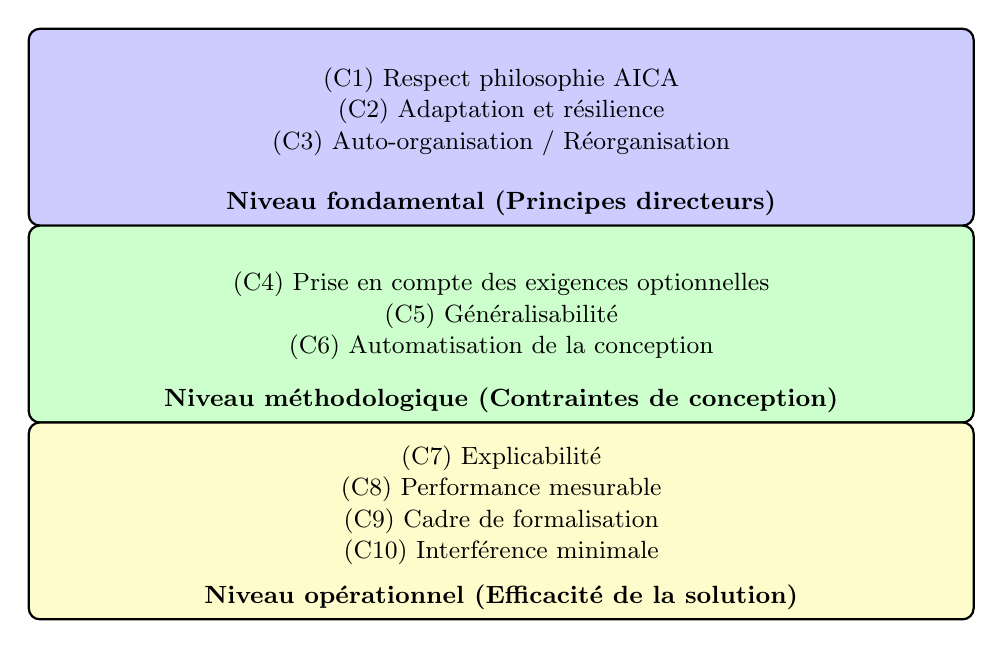
\begin{tikzpicture}[
        levelbox/.style={draw, rounded corners, thick, minimum width=12cm, fill=#1!20},
        itemtext/.style={align=center, font=\small},
        titletext/.style={font=\bfseries\small, yshift=0.3cm},
        node distance=0.4cm
    ]

    % NIVEAU FONDAMENTAL
    \node[levelbox=blue, minimum height=2.5cm] (fundamental) at (0, 5) {};
    \node[titletext, align=center] at (fundamental.south) {Niveau fondamental (Principes directeurs)};
    \node[itemtext] at (0, 5.6) {(C1) Respect philosophie AICA};
    \node[itemtext] at (0, 5.2) {(C2) Adaptation et résilience};
    \node[itemtext] at (0, 4.8) {(C3) Auto-organisation / Réorganisation};

    % NIVEAU MÉTHODOLOGIQUE
    \node[levelbox=green, minimum height=2.5cm] (methodo) at (0, 2.5) {};
    \node[titletext, align=center] at (methodo.south) {Niveau méthodologique (Contraintes de conception)};
    \node[itemtext] at (0, 3.0) {(C4) Prise en compte des exigences optionnelles};
    \node[itemtext] at (0, 2.6) {(C5) Généralisabilité};
    \node[itemtext] at (0, 2.2) {(C6) Automatisation de la conception};

    % NIVEAU OPÉRATIONNEL
    \node[levelbox=yellow, minimum height=2.5cm] (operationnel) at (0, 0) {};
    \node[titletext, align=center] at (operationnel.south) {Niveau opérationnel (Efficacité de la solution)};
    \node[itemtext] at (0, 0.8) {(C7) Explicabilité};
    \node[itemtext] at (0, 0.4) {(C8) Performance mesurable};
    \node[itemtext] at (0, 0) {(C9) Cadre de formalisation};
    \node[itemtext] at (0, -0.4) {(C10) Interférence minimale};

\end{tikzpicture}

%     }
%     \caption{Hiérarchie des critères guidant la conception d'un SMA de Cyberdéfense (de type AICA)}
%     \label{fig:criteria}
% \end{figure}

Nous nous appuyons sur un ensemble de critères, résumée en \autoref{tab:critere_hierarchie}, décrivant les propriétés qu’un \acn{SMA} de Cyberdéfense doit satisfaire pour répondre à la question de recherche globale.

\begin{table}[H]
  \centering
  \caption{Grille des critères répondant à la question globale}
  \label{tab:critere_hierarchie}
  \small
  \renewcommand{\arraystretch}{1.12}
  \begin{tabular}{ccp{5cm}}
    \hline
    \textbf{Niveau} & \textbf{Critère} & \textbf{Nom}                              \\
    \hline
    \multirow{4}{*}{Fondamentaux}
                    & \textbf{C1}      & Autonomie distribuée.                     \\
                    & \textbf{C2}      & Couverture fonctionnelle (P3R3)           \\
                    & \textbf{C3}      & Capacité d’adaptation                     \\
                    & \textbf{C4}      & Respect des contraintes / sûreté          \\
    \hline
    \multirow{3}{*}{Exploitabilité}
                    & \textbf{C5}      & Explicabilité et contrôle organisationnel \\
                    & \textbf{C6}      & Résilience / tolérance aux défaillances   \\
                    & \textbf{C7}      & Mesurabilité des performances             \\
    \hline
    Soutenabilité
                    & \textbf{C8}      & Coût de conception minimal                \\
    \hline
  \end{tabular}
\end{table}

\noindent
Le premier niveau est \textbf{fondamental} car il regroupe les critères indispensables à toute solution qui prétend répondre à la question de recherche globale. Le critère \textbf{C1 (Autonomie distribuée)} exprime le principe des \acn{SMA} dans lequel plusieurs agents autonomes coopèrent localement sans supervision centrale. Cette autonomie distribuée est cruciale dans un contexte cyber où la réactivité locale et la scalabilité du système sont des exigences fortes. Le critère \textbf{C2 (Couverture fonctionnelle P3R3)} exige que le \acn{SMA} ne se limite pas à la détection d’attaques, mais soit également capable d'y répondre et de restaurer le système, conformément aux trois fonctions identifiées dans le modèle P3R3. Le critère \textbf{C3 (Capacité d’adaptation)} évalue la faculté du \acn{SMA} à s’ajuster dynamiquement face à des perturbations internes ou à des changements de l’environnement. Cette adaptation peut être rendue possible via des mécanismes d’auto-organisation ou de réorganisation, en lien avec des besoins émergents. Le critère \textbf{C4 (Respect des contraintes / sûreté)} impose que le comportement des agents soit conforme à un ensemble de règles explicites (qu’elles soient de nature fonctionnelle, réglementaire, ou de sécurité) et qu’il n’engendre pas de comportements indésirables ou dangereux pour le système global.

Le deuxième niveau, dit d’\textbf{exploitabilité}, regroupe les critères qui rendent l’usage du \acn{SMA} viable, interprétable et maintenable dans le temps. Le critère \textbf{C5 (Explicabilité et contrôle organisationnel)} fait référence à la capacité à comprendre, expliquer et superviser les comportements collectifs du \acn{SMA}, tant du point de vue des ingénieurs que des opérateurs humains. Un système difficilement compréhensible d'un point de vue organisationnelle empêche son amélioration et sa fiabilisation. Le critère \textbf{C6 (Résilience / tolérance aux défaillances)} souligne l’importance d’une robustesse structurelle du \acn{SMA} : il doit pouvoir continuer à fonctionner, même partiellement, en cas de panne d’un agent ou d’un sous-système, pour garantir une continuité minimale de la cyberdéfense. Le critère \textbf{C7 (Mesurabilité des performances)} stipule que les performances du système doivent pouvoir être quantifiées dans un cadre formel afin de permettre l’évaluation, la comparaison entre approches, et l’amélioration incrémentale des solutions proposées.

Enfin, le niveau de \textbf{soutenabilité} introduit le critère \textbf{C8 (Coût de conception minimal)} qui mesure la capacité d’une méthode à limiter l’effort d’ingénierie requis pour spécifier, concevoir, et ajuster un \acn{SMA} de cyberdéfense. Dans un contexte opérationnel, les ressources humaines et temporelles sont limitées, ce qui rend la réduction du coût de conception (notamment par l’automatisation ou la réutilisabilité) un facteur déterminant pour le passage à l'échelle.

\clearpage
\thispagestyle{empty}
\null
\newpage


\chapter{Vers des SMA de Cyberdéfense et leur conception}

% TODO~: A utiliser pour compléter "Vers des approches multi-agents de Cyberdéfense"
% % \usepackage{amsmath,amssymb,amsfonts}
% \usepackage{algorithmic}
% \usepackage{graphicx}
% \usepackage[inline]{enumitem}
% \usepackage{tabularx}
% \usepackage{caption}
% \usepackage[T2A,T1]{fontenc}
% \usepackage[french]{babel}
% \captionsetup{font=it}
% \usepackage{ragged2e}
% \usepackage{hyperref}
% \usepackage{footmisc}
% \usepackage{booktabs}
% \usepackage{smartdiagram}
% \usepackage{textcomp}
% \usepackage{xcolor}
% \def\BibTeX{{\rm B\kern-.05em{\sc i\kern-.025em b}\kern-.08em
%     T\kern-.1667em\lower.7ex\hbox{E}\kern-.125emX}}
% \usepackage{cite}

% \usepackage{etoolbox}
% \patchcmd{\thebibliography}{\section*{\refname}}{}{}{}

% \setlength{\extrarowheight}{2.5pt}


\section{Introduction}

% Le contexte
% Alors que de plus en plus de réseaux et d'appareils connectés sont utilisés, en particulier dans l'<<~Internet of Things~>> (IoT) et l'<<~Internet of Battle Things~>> (IoBT), le besoin de leur propre sécurité est devenu un défi très important. Les systèmes tels que les capteurs sans fil ou les véhicules autonomes ont une surface d'attaque accrue, car ils offrent de nouveaux vecteurs d'attaque pour corrompre, détruire et propager de nouvelles cyber-attaques sur les réseaux connectés.
%\cite{ccdc_army_research_laboratory_internet_2017}.


Le développement de l'<<~Internet of Things~>> et de l'<<~Internet of Battle Things~>>  a entrainé une augmentation de la surface d'attaque des systèmes en réseau permettant à des attaquants de s'y introduire en ciblant les nœuds les plus faiblement défendus. Tenant compte de ce contexte, le groupe de travail <<~AICA IWG~>>\footnote{Ce groupe de travail (voir \url{https://www.aica-iwg.org/}) s'appuie sur les résultats du \textit{Research Task Group IST-152} de l'OTAN qui a travaillé sur le concept des <<~Intelligent, Autonomous and Trusted Agents for Cyber Defense and Resilience~>>.} a poursuivi le développement des travaux concernant l'agent AICA (Autonomous Intelligent Cyber-defence Agent).
Un agent est par définition une entité autonome capable de percevoir son environnement local grâce à des capteurs, et d’agir sur cet environnement à l'aide d'effecteurs\cite{russell1995modern}.
L'agent AICA doit pouvoir être déployé sur un système hôte pour détecter, identifier et caractériser des anomalies/attaques, élaborer et piloter l’exécution de contre-mesures et dialoguer avec l'extérieur. À cette fin, il est conçu comme proactif, discret et capable d’apprendre.

% \noindent



L'agent AICA peut être vu comme un Système Multi-Agent (SMA). Le paradigme multi-agent offre des moyens de gérer l'ouverture, le passage à l'échelle et l'autonomie du système hôte en déléguant différents aspects de la cyber-défense à différents agents. L'agent AICA  est alors un système collectif décentralisé et distribué d'agents cyber-défenseurs déployés au plus près des composants du système\cite{ieeesp_KottT20}.
%Évitant l'écueil d'un point de défaillance unique, ils contribuent aussi à opposer plusieurs couches de cyber-défense à un éventuel cyber-attaquant.

Concevoir un tel SMA, nécessite de porter une attention particulière à son organisation. L'objectif de cet article est de discuter des mécanismes organisationnels d'un SMA de cyberdéfense.
% Cet article aborde des mécanismes organisationnels disponibles pour concevoir un SMA qui répond à des objectifs de cyber-défense ainsi qu'aux contraintes du système hôte de déploiement.
% Notre intérêt porte principalement sur la protection des systèmes en réseau dont les nœuds peuvent héberger des agents.% aussi bien sur des réseaux mobiles que sur des réseaux fixes.
% La recherche de recommandations et/ou pistes de conception pour ce SMA s'appuie sur une revue des différentes organisations disponibles avec leurs objectifs de cyber-défense et systèmes hôtes associés.
% Structure & Méthode
La section II introduit un état de l'art de SMA existants assurant la cyber-défense sur leur système hôte. La section III identifie les verrous théoriques et techniques potentiels vers la conception d'un SMA de cyber-défense auto/ré-organisé et propose des préconisations.

% REMARQUE : plutôt que edt mettre uniquement "Travaux liés"
\section{\'Etat de l'art}

\subsection{Vers des systèmes multi-agents de cyber-défense}


% % Expliquer à quels défis de sécurité nous devons initialement faire face...
% Le monde du cyber
% % dans lequel opère tout système fournissant une couverture de sécurité
% rassemble une grande variété de définitions et de termes issus de plusieurs domaines\cite{bjorck2015cyber}. Le terme \textbf{cyber} fait référence à toutes les activités liées à une utilisation offensive ou défensive du cyberespace\cite{nocetti2018darkening}.

Nous inscrivant dans le prolongement des travaux menés dans le cadre de l'AICA IWG, nous considérons la \textbf{cyber-sécurité} comme l'ensemble des activités  consistant à se protéger de façon préventive contre les cyber-attaques\cite{theron_autonomous_2021}.


Nous désignons par \textbf{cyber-défense}  l'ensemble des activités entreprises lorsqu'une cyber-attaque est détectée et qu'il faut réagir. Ces activités sont décrites dans le cadre du <<~P3R3 Resilience Engineering Framework~>>\cite{Theron2013P3R3} et sont regroupées en trois fonctions de cyber-défense :

\noindent
\textit{\textbf{R1 - Detect and alarm}} : détection des cyber-attaques  et déclenchement des mécanismes de réponse; %Cela couvre également la surveillance du système à défendre et l'avertissement d'éventuelles cyber-attaques.

\noindent
\textit{\textbf{R2 - Respond and restore}} : mise en œuvre et suivi des réponses apportées aux cyber-attaques et l restauration des niveaux de services/activités minimaux. La gestion de la crise provoquée par l'attaque est au cœur de cette fonction;

\noindent
\textit{\textbf{R3 - Recover and rebound}} : rétablissement des parties endommagées du système à défendre et traitement final des conséquences. Ce point inclut une phase d'apprentissage permettant l'amélioration du système de cyber-défense.

% \begin{figure}[ht!]
%     \centering
%     \smartdiagramset{back arrow disabled=true}
%     \smartdiagram[flow diagram:horizontal]{\textbf{(R1)} Detecter \& Alarmer, \textbf{(R2)} Répondre \& Restaurer, \textbf{(R3)} Rétablir \& Rebondir}
%     \caption{Cadre fondamental de travail pour la cyber-défense (tiré de \cite{Theron2013P3R3})}
%     \label{fig:framework_r3}
% \end{figure}

%(contrecarrer une cyber-attaque après qu'elle a réussi)

%(en prévention d'une cyber-attaque) \cite{theron_autonomous_2021}.
% Les deux sont importants pour assurer la \textbf{cyber résilience}\cite{theron_autonomous_2021}.
% Nous choisissons d'inclure les objectifs de cyber-défense, de cyber-sécurité et de cyber résilience dans le même terme d'\textbf{objectif de cyber-défense}.

Nous appelons \textbf{objectifs de cyber-défense}, tous les objectifs impliquant la mise en œuvre d'une ou plusieurs des %\old{activités} 
fonctions de cyber-défense.

% qui ont pour finalité de garantir des critères de sécurité sans perturber la productivité du système défendu dans le cas où une cyber-attaque a eu lieu\cite{keyser2018information}. Sur la base de la norme ISO 25010, des triades CIA (Confidentiality, Intégrity, Availability) et AAA (Authentication, Availability, Accountability), nous avons choisi la recherche de la confidentialité, l'intégrité, la disponibilité, la responsabilité et la non-répudiation comme cadre initial fondamental de nos objectifs de cyber-défense.%\cite{iso25010}.

% Un tel système repose sur la répartition de la responsabilité de la sécurité entre plusieurs agents. Ces agents peuvent être conçus pour surveiller différents aspects du système, tels que le trafic réseau, l'activité des utilisateurs et les journaux système, et pour prendre les mesures appropriées lorsque des cyber-menaces sont détectées.
% Un SMA peut inclure des agents chargés d'identifier et de bloquer le trafic malveillant, des agents qui surveillent l'activité des utilisateurs et détectent les comportements suspects, et des agents qui analysent les journaux système et alertent les administrateurs des problèmes de sécurité potentiels.
% L'utilisation de plusieurs agents peut améliorer la sécurité du système hôte de plusieurs façons. Premièrement, cela permet une approche plus globale de la sécurité, car différents agents peuvent se concentrer sur différents aspects du système. Deuxièmement, cela peut réduire le risque d'un point de défaillance unique, car la défaillance d'un agent ne compromettra pas nécessairement la sécurité de l'ensemble du système. Enfin, l'utilisation de plusieurs agents peut rendre plus difficile pour un attaquant de compromettre le système, car il devrait contourner plusieurs couches de cyber-défense.

% \textbf{La confidentialité} est la capacité d'un système à ne pas rendre les données accessibles aux personnes non autorisées\cite{noauthor_glossaire_nodate} ;
% % (via le chiffrement, les règles et politiques de contrôle d'accès, l'authentification, la gestion des autorisations qui limite les actions possibles selon des règles).

% \textbf{L'intégrité} est la capacité d'un système à se protéger des modifications non autorisées\cite{noauthor_glossaire_nodate} ;
% % (via les sauvegardes, les sommes de contrôle, le contrôle de version, les journaux de données, les erreurs de données et les codes de correction).

% \textbf{Disponibilité} est "la capacité d'un élément/entité à pouvoir exécuter une fonction requise dans des conditions données, à un moment donné ou pendant un intervalle de temps donné, en supposant que les ressources externes nécessaires sont fournies"\cite{ afnor_norme_nodate} ;
% % (au travers des protections physiques, de la redondance et du plan de continuité et de reprise des données).

% \textbf{Non-répudiation} qui est la capacité d'un système à prouver qu'une action a bien été appliquée\cite{25010_2011} ;

% \textbf{Responsabilité} qui est la capacité d'un système à retracer les actions avec ceux qui sont derrière elles\cite{1400-1700_isoiec_nodate}.
% elle inclut la \textbf{traçabilité} car c'est "la capacité à suivre la vie d'une exigence, depuis ses origines, en passant par son développement, ses spécifications, son déploiement et son utilisation"\cite {gotel_analysis_1994} ; et \textbf{authenticité} qui est la capacité d'un système à apporter la preuve de son identité\cite{noauthor_glossaire_nodate}.


% montrant que ces problèmes sont résolus par la sécurité collaborative...
% \subsection{cyber-sécurité collaborative via des SMA}


% la sécurité collaborative qu'on défini comme...
% notion de sécurité collaborative sujette à caution...
%\old{[[Supprimé]]La littérature fournit le concept de \textbf{sécurité collaborative} impliquant plusieurs parties techniques et non techniques dans le processus d'identification, de prévention et de réponse aux cyber-menaces sur des infrastructures\cite{meng2015collaborative}.}
% Cela implique, entre autres, le partage d'informations, de ressources et d'expertise afin d'améliorer l'efficacité et l'efficience des mesures de cyber-sécurité et cyber-défense\cite{meng2015collaborative}.

% technique : logiciel et matériel
% SOC central insuffisant...
%\old{[[Supprimé:]]Inspirés par ce paradigme, nous définissons la \textbf{cyber-défense collaborative} comme la poursuite d'objectifs de cyber-défense par plusieurs entités logicielles réagissant aux cyber-attaques ciblant un système vu comme un réseau de nœuds.}
% todo : expliciter la finalité

Dans un \textbf{SMA de cyber-défense}, plusieurs agents atteignent un objectif global de cyber-défense par un comportement collectif résultant de la réalisation de sous-objectifs individuels et/ou de mécanismes locaux\cite{jamont2015meeting}. Des exemples de tels sous-objectifs pourraient être la détection des intrusions, la mise en œuvre d'un plan de récupération, la restauration d'une image, redirection des ports\dots

% Selon la référence \cite{boissier2004caractéristiques}, les SMA sont :
% autonome (la prise de décision ne dépend pas d'une entité externe) ; répartis (les connaissances ou les tâches sont réparties dans chaque agent) ; décentralisé (la responsabilité d'atteindre un objectif est confiée à tous les agents) ; situé dans l'environnement (espace commun où interagissent les agents \cite{odell2002modeling}) ; permettre des interactions entre agents (action réciproque de deux ou plusieurs entités\cite{noauthor_interaction_nodate} pouvant conduire à des stratégies de coopération, collaboration, compétition, négociation entre les agents) en utilisant la communication (assurer une cohérence globale malgré la décentralisation en utilisant un langage grammaticalement structuré, utiliser d'un protocole spécifique, utilisation d'un espace commun ou "tableau noir"); montrant l'émergence (résultat du comportement des agents individuels à travers leurs interactions\cite{di2005self}) ; et avoir une organisation (en tant que modèle global éventuellement défini a priori ou en tant que phénomène émergent\cite{salvador2019multi}).


\subsection{Mécanismes organisationnels dynamiques}

L'autonomie de fonctionnement du SMA de cyber-défense, obtenue  en déléguant aux agents certaines missions % avec peu d'interventions directes, 
est une réponse face aux charges de travail des équipes cyber et à la rapidité des cyber-attaques\cite{ieeesp_KottT20}.
Un tel SMA doit modifier sa structure et les relations entre ses agents pour continuellement s'adapter à son environnement \cite{theron_autonomous_2021}.
%La réorganisation et l'auto-organisation sont alors des mécanismes clés  \cite{picard2009reorganisation}.

% De plus, comme discuté dans \cite{theron_autonomous_2021}, nous avançons l'hypothèse que les mécanismes d'organisation assurant la sécurité sont susceptibles de nécessiter un bon niveau de représentation et de conscience de l'environnement pour un processus de prise de décision et d'apprentissage complexe précis.

% La \textbf{réorganisation} est définie comme un processus descendant imposant une organisation (vue comme une entité distincte) aux agents. Ces mécanismes de réorganisation sont inclus dans l'Organisation-Centered Point Of View (OCPV)\cite{picard2009reorganisation}. Dans l'OCPV, la sécurité globale est une tâche commune partagée par tous les agents à travers leur organisation. Il s'avère être un moyen de basculer entre plusieurs organisations éprouvées qui semblent adaptées dans des circonstances données.
% À une faible conscience environnementale/organisationnelle, une organisation basée sur OCPV peut être codée en dur en tant que règles de sécurité à suivre dans les agents eux-mêmes.
% Avec un niveau de conscience environnementale et/ou organisationnelle plus élevée, une organisation basée sur l'OCPV est partagée comme une représentation globale (topologie) par tous les agents qui peuvent la modifier directement par des processus sociaux.
% Selon \cite{picard2009reorganisation}, de tels SMA sont dits "\textbf{organization oriented}". Les rôles et cahiers des charges qui composent l'organisation sont à faire évoluer par les agents eux-mêmes (ou des entités extérieures) lorsque l'organisation n'est pas adaptée en travaillant directement sur des schémas de coopération et d'organisation \cite{picard2009reorganisation}.

% \textbf{L'auto-organisation} est définie comme un processus ascendant où l'organisation résulte des interactions et des actions locales des agents comme un phénomène émergent. Les mécanismes d'auto-organisation appartiennent à l'Agent-Centered-Point-Of-View (ACPV)\cite{picard2009reorganisation}. Dans l'ACPV, la sécurité globale résulte des actions de sécurité locales et des interactions pair à pair entre les agents. C'est un moyen efficace de faire face aux cyber-menaces sans avoir besoin d'un contrôle ou d'un guidage central.
% À une faible conscience environnementale/organisationnelle, une organisation basée sur l'ACPV est conçue pour réagir au déclenchement de combinaisons d'événements de sécurité pour appliquer des actions cartographiées. Il convient de noter que la notion récurrente d'"intelligence en essaim" est incluse dans ce cas car il n'y a aucune connaissance de l'organisation pour les agents.
% Avec un niveau de conscience environnementale et/ou organisationnelle plus élevée, une organisation basée sur l'ACPV tire parti de la représentation locale intégrée de l'environnement direct de l'agent (agents cyber-défenseurs voisins, nœuds de réseau découverts, processus en cours d'exécution, etc.) pour un processus cognitif.
% Selon \cite{picard2009reorganisation}, de tels SMA sont dits "\textbf{coalition based}". Les dépendances/relations inter-agents sont modifiées par les agents eux-mêmes en raison d'une inadéquation en modifiant les schémas de coopération ou indirectement l'organisation.

En considérant un point de vue centré organisation, la cyber-défense globale est une tâche commune partagée par tous les agents à travers leur organisation. La \textbf{ré-organisation} est un moyen de basculer entre plusieurs organisations éprouvées qui semblent adaptées dans des circonstances données\cite{picard2009reorganisation}.

En considérant un point de vue centré agent, l’\textbf{auto-organisation} est définie comme un processus ascendant où l’organisation émerge des interactions et des actions locales des agents. La cyber-défense globale résulte alors des actions de cyber-défense locales et des interactions pair à pair entre les agents\cite{picard2009reorganisation}. L'auto-organisation semble être un des moyens à mobiliser pour faire face aux cyber-menaces en évitant les écueils d'un contrôle centralisé.



\begin{table*}[t!]

    \caption{Un aperçu de quelques organisations et des environnement hôtes utilisés dans les SMA de cyber-défense étudiés}

    \begin{tabularx}{\linewidth}{
            >{\raggedright\arraybackslash\hsize=.3\hsize}X
            >{\raggedright\arraybackslash\hsize=.6\hsize}X
            >{\raggedright\arraybackslash\hsize=.6\hsize}X
            >{\raggedright\arraybackslash\hsize=.6\hsize}X
            % >{\raggedright\arraybackslash}X
            >{\raggedright\arraybackslash\hsize=.2\hsize}X}
        \toprule

        { \textbf{Organisation}}
         & {  \textbf{Avantages principaux}}
         & {  \textbf{Inconvénients principaux}}
         & {  \textbf{Environnement}}
        % & {  \textbf{ Objectifs de cyber-défense suggerés }}
         & {  \textbf{Travaux}}
        \\ \midrule

        { Centralisé}
         & {  Haute précision pour l'analyse de la situation}
         & {  Single-Point-Of-Failure (SPOF), manque de scalabilité}
         & {  Petit à moyenne taille, non ouvert, petite entreprise}
        % & {  \textbf{Objectifs de type (R1)} : détection d'intrusion, surveillance du réseau}
         & {  \cite{vasilomanolakis2015taxonomy, gorodetski2003multi, de2017distributed}}
        \\

        { Hiérarchique (distribué)}
         & {  Évolutivité, décomposition des tâches}
         & {  Perte d'informations, goulots d'étranglement, retards}
         & {  Taille moyenne à grande, ouvert, peu de variations}
        % & {  \textbf{Objectifs de type (R1) et (R2)} : surveillance du réseau, sauvegardes régulières, contrôles d'accès, correctifs de cyber-défense}
         & {  \cite{holloway2009self, lamont2009military}}
        \\

        { Décentralisé (Peer-to-Peer)}
         & {  Structure non définie a priori, Hautement adaptatif}
         & {  Contrôle de l'organisation limitée, intensité de communication}
         & {  Ouvert, toute taille, fortes variations}
        % & {  \textbf{Objectifs de type (R3)} : reconnaissance de menaces, adaptation aux cyber-attaques}
         & {  \cite{holloway2019self, haack2011ant, morteza2015method}}
        \\

        { Coalition}
         & {  Optimisation de l'organisation autour des tâches}
         & {  Peu adapté sur le long terme}
         & {  Toute taille, ouvert, peu de variations, peu de ressources}
        % & {  \textbf{Objectifs de type (R3)} : contre-mesures de sécurité adaptées, apprentissage des cyber-attaques}
         & {  \cite{carvalho2011evolutionary}}
        \\

        { Équipes}
         & {  Bonne performance pour des tâches régulières}
         & {  Haute intensité de communication}
         & {  Ouvert, hétérogène, toute taille, peu de variations}
        % & {  \textbf{Objectifs de type (R1) et (R2)} : détection de menaces possibles, application de contre-mesures}
         & {  \cite{akandwanaho2018generic}}
        \\

        { Marché}
         & {  Organisation optimisée par concurrence, bonne gestion des agents}
         & {  Processus d'allocation complexe et long}
         & {  Toute taille, ouvert, peu de variations, peu de ressources}
        % & {  \textbf{Objectifs de type (R3)} : investigations forensiques, stratégies de cyber-défense}
         & {  \cite{demir2021adaptive}}
        \\
        \bottomrule
    \end{tabularx}
    \label{tab:general-overview}
\end{table*}


\subsection{Organisations des SMA de cyber-défense}


Le choix d'une organisation de SMA de cyber-défense implique de tenir compte des relations entre les objectifs de cyber-défense et l'environnement de déploiement. L'analyse des SMA de cyber-défense disponibles est susceptible d'indiquer des tendances pour ces relations. Cela permettrait de favoriser la mise en œuvre d'une organisation à partir des objectifs de cyber-défense et l'environnement de déploiement.

%Pour établir cette revue de littérature, nous avons procédé à une recherche automatisée sur la base de mots clés liés, d'un côté, aux SMAs, et d'un autre côté, au monde de la sécurité logicielle s'inscrivant dans la définition donnée précédemment de la cyber-défense.
% Nous avons utilisé plusieurs bases de donnée électroniques tels que \cite{ACM,IEEE,Elsevier,Springer}.
%Puis nous avons effectué une lecture des résumés pour obtenir finalement une vingtaine de publications\footnote{Toutes les références n'ont pas pu être données en raison du format} s'inscrivant dans le cadre d'un SMA devant remplir un objectif de cyber-défense. Pour chaque proposition de SMA, nous avons suggéré une classification des informations en déterminant la caractéristique principale de l'organisation, l'environnement de déploiement ainsi que les objectifs de cyber-défense. Pour chacune des organisations identifiées, nous avons aussi suggéré des avantages et inconvénients généraux. Un aperçu de ce travail est à la table \ref{tab:general-overview}.

%% MO: j'ai reformulé, car ça faisait vraiment amateur :))
Notre revue de littérature s'est concentrée sur le rapprochement des notions des SMA et de la cyber-défense.

Pour chacun des travaux de SMA de cyber-défense, nous nous sommes intéressés aux fonctions de cyber-défense couvertes. Un aperçu de cette classification est proposé en table \ref{tab:reference-cyberdefense}. %\footnote{Les références des travaux exploités ne sont pas citées dans ce tableau en raison du format.}\label{notallrefs. 
Nous avons constaté que la plupart des objectifs de cyber-défense des SMA se concentrent principalement sur la détection d'anomalies et d'intrusions (plus de 50\% des travaux de notre revue complète se focalisent ainsi sur la fonction R1).

\begin{table}[htb]

    \caption{Un aperçu des fonctions de cyber-défense prises en charge par les SMA de cyber-défense étudiés}

    \begin{tabularx}{0.49\textwidth}{
            >{\raggedright\arraybackslash\hsize=.9\hsize}X
            >{\raggedright\arraybackslash\hsize=.3\hsize}X}
        \toprule

        { {\textbf{Objectifs principaux}}}
         & {  \textbf{Travaux}}
        \\ \midrule

        {  \textbf{\textbf{R1}}: détection d'intrusion, surveillance du réseau, détection de menaces possibles}
         & {  \cite{vasilomanolakis2015taxonomy, gorodetski2003multi, de2017distributed, holloway2009self, lamont2009military, akandwanaho2018generic}}
        \\

        {  \textbf{\textbf{R2}}: application de contre-mesures, contrôles d'accès, correctifs de cyber-défense, stratégies de cyber-défense}
         & {  \cite{holloway2009self, lamont2009military, akandwanaho2018generic}}
        \\

        {  \textbf{\textbf{R3}}: investigations forensiques, élaboration de contre-mesures adaptées, apprentissage des cyber-attaques, adaptation aux cyber-attaques}
         & {  \cite{holloway2019self, haack2011ant, morteza2015method, demir2021adaptive}}
        \\
        \bottomrule
    \end{tabularx}
    \label{tab:reference-cyberdefense}
\end{table}


Pour chacun de ces mêmes travaux, nous nous sommes aussi intéressés aux caractéristiques principales de l’organisation et de l'environnement de déploiement. Un aperçu de ce travail est présenté en table \ref{tab:general-overview} %\footref{notallrefs}.
Nous constatons qu'indépendamment des objectifs de cyber-défense, l'organisation centralisée et/ou hiérarchique est la plus répandue parmi les SMA de cyber-défense étudiés. La centralisation des données acquises de l'environnement, en un seul point, favorise de meilleures performances pour l'analyse de la situation globale et le contrôle du système de cyber-défense. Ces types d'organisation semblent moins facilement s'appliquer pour des réseaux dynamiques, mais sont répandus sur des systèmes de taille moyenne avec des contraintes connues\cite{vasilomanolakis2015taxonomy}.
%
%\noindent
Les organisations de type décentralisé tirent profit d'une approche davantage auto-organisée pour faire face aux cyber-menaces de façon à augmenter l'autonomie du SMA de cyber-défense comme proposé dans le <<~Artificial Immune System~>> \cite{morteza2015method} ou la <<~Ant-Based Cyber Security~>> \cite {haack2011ant}.% en sont des exemples. %Elles sont néanmoins moins établies en tant que solutions génériques de cyber-défense et/ou cyber-sécurité.

% bien qu'elles ne soient pas bien établies (dans les organisations décentralisées).
% Finalement, les coalitions sont d'autres organisations récurrentes utilisées pour tirer parti de leurs principaux avantages lors de la distribution et du traitement des tâches pour atteindre des objectifs spécifiques dans un environnement caractéristique.


\section{Vers un mécanisme général d'organisation de la cyber-défense en réseau}

La revue a permis d'identifier de premiers mécanismes sous-jacents à un SMA de cyber-défense. Cependant, il est nécessaire de la compléter par une étape d'expérimentation.
En effet, notre classification ne permet pas de définir de façon certaine des recommandations de conception d'organisation pour un SMA de cyber-défense générique. La diversité (des objectifs, des environnements, des architectures d'agents, des protocoles d'interaction\dots) des SMA de cyber-défense disponibles rend l'appréciation entre ces derniers difficiles sans cadre commun.

\subsection{Vers un modèle expérimental de la situation}
% titre de sous section pas super explicite je trouve

Il apparaît nécessaire de caractériser le SMA de cyber-défense
% (y compris son organisation, ses objectifs et ses performances)
et l'environnement dans lequel il est déployé.% avec ses propriétés
% (y compris probablement des métriques)
%en connaissant les actions de cyber-défense/attaque qui peuvent l'impacter. 

Un  modèle générique  permettrait alors de représenter des scénarios d'attaque sur un environnement réseau avec un ou pour plusieurs types de SMA de cyber-défense. Cependant, aucun des travaux étudiés ne répond précisément à ce besoin. Sa mise en œuvre prendrait la forme d'un simulateur de réseau sur lequel seraient déployés plusieurs agents d'attaque et défense. Cependant, les simulateurs de réseau du domaine les plus aboutis ne permettent d'avoir qu'un seul agent d'attaque ou de défense là où nous souhaiterions évaluer le passage à l'échelle des SMA de cyber-défense.


% Ce modèle pourrait être développé comme un Decentralized Partially Observable Markov Decision Process (Dec-POMDP) car l'environnement, les agents et les actions car le problème repose sur une prise de décision prenant en compte l'incertitude et les observations
% ... expliciter le choix d'un dec POMDP , à voir (citation)


Pour répondre à ce besoin, il serait possible d'étendre un modèle générique de réseau pouvant subir une cyber-attaque, tel que dans le simulateur CYST\cite{drasar_session-level_2020},
%ou \cite{cyberbattlesim}
avec la possibilité d'avoir plusieurs agents d'attaque et de cyber-défense. Un tel modèle serait la base d'un simulateur qui permettrait un grand nombre de possibilités expérimentales pour appréhender l'impact de l'organisation des agents de cyber-défense.

% Une piste pour implémenter ce simulateur est de s'appuyer sur le framework <<~PettingZoo~>>\cite{terry2020pettingzoo} qui est adapté pour le contexte .
% expliciter pourquoi pettingZoo

\subsection{Traitement des facteurs pour concevoir des organisations}

Dans notre contexte, la conception d'une organisation d'un SMA de cyber-défense est un processus prenant en compte les facteurs suivant : les contraintes matérielles et logicielles de l'environnement de déploiement;
% (supposé être partiellement défini par l'utilisateur et/ou la politique établie)
les menaces internes du SMA de cyber-défense lui-même; et les modèles définis d'architecture et d'objectifs de cyber-défense.

Actuellement, il n'existe pas de méthodes ou de processus automatisés visant à trouver un consensus avec ces facteurs lors de la conception d'une organisation.
La conception d'un SMA de cyber-défense auto/ré-organisé repose alors sur l'expérience empirique du concepteur en suivant des exigences définies.
Une autre approche serait de s'appuyer sur des mécanismes automatisés pour développer une organisation adaptée avec peu d'intervention du concepteur.
Une première piste serait le <<~Distributed Constrained Optimization Problem~>> (DCOP) où les facteurs d'organisation seraient modélisés par une fonction de coût que cherchent à minimiser \textit{online} les agents cyber-défenseurs en s'organisant. Une deuxième voie serait le <<~Multi-Agent Reinforcement Learning~>> (MARL) où les agents cyber-défenseurs apprennent eux-mêmes les organisations possibles adaptées par rapport à une récompense reçue modélisant les objectifs de cyber-défense.

\section{Conclusion}
Un SMA de cyber-défense déployé sur un système hôte en réseau permettrait de relever les défis liés à la complexité et la rapidité de cyber-attaques. Notre étude donne un aperçu d'organisations possibles respectant des objectifs de cyber-défense et des contraintes de l'environnement de déploiement d'un SMA de cyber-défense.
Elle souligne aussi le besoin de définir un cadre théorique et technique spécifique à l'organisation d'un SMA de cyber-défense dans un environnement réseau. Un tel cadre permettra d'explorer, d'évaluer et de tirer des recommandations sur l'organisation d'un SMA de cyber-défense que nous valoriserons pour le développement d'un agent AICA.

\noindent
Ce chapitre situe notre démarche au regard des travaux existants à l'intersection des domaines de la Cyberdéfense, \acn{SMA}. Il repose sur une revue de littérature menée au début de la thèse et mise à jour tout au long des travaux.
%
Nous adoptons une lecture critique orientée par les huit critères de conception (C1 à C8) identifiés au chapitre précédent. Cette lecture permet de structurer les contributions existantes selon leur degré de proximité avec la vision d'un \acn{SMA} de Cyberdéfense.

Nous distinguons pour cela deux axes complémentaires. Le premier (\autoref{sec:sma-cyberdefense}) s’intéresse aux \textbf{SMA existants appliqués à la cyberdéfense}, en examinant les objectifs pris en charge, les types d’organisation, et les environnements de déploiement associés. Le second (\autoref{sec:sma-cyberdefense-conception}) explore les \textbf{moyens existants pour concevoir ces SMA}, qu’ils soient manuels ou automatisés, symboliques ou apprenants
%
Les travaux identifiés concernant l'idée d'agents autonomes ou même de défense distribuée doivent prendre en compte simultanément tous les critères identifiées précédemment.


\section{Les SMA de Cyberdéfense dans la littérature$^{1}$}\label{sec:sma-cyberdefense}

\footnotetext[1]{Ce paragraphe s'appuie sur une revue de littérature initialement publiée dans \autocite{soule2023ressithese}.}

Un \acn{SMA} de Cyberdéfense demande de prendre en considération les enjeux de structuration, d'adaptabilité et de coordination dans un environnement critique et dynamique.
Dans un premier temps, nous avons conduit une revue de littérature des travaux pouvant se comparer aux \acn{SMA} de Cyberdéfense~\cite{soule2023ressithese}.
En particulier, pour chacun des travaux identifiés, nous avons étudié le rapport entre le mécanisme d'organisation adopté et les \textbf{objectifs de cyber-défense} impliquant la mise en œuvre d'une ou plusieurs des fonctions de cyber-défense tels que décrit dans le P3R3~\cite{Theron2013P3R3}~:
(R1) Détection des intrusions et alertes,
(R2) Application de contre-mesures et rétablissement minimal,
(R3) Apprentissage post-attaque et amélioration continue.
Cette première étude permet une revue des travaux identifiés au travers de la grille d'analyse fondée sur les critères identifiés en \autoref{sec:problematique-sma}.

Dans un \textbf{SMA de cyber-défense}, plusieurs agents atteignent un objectif global de cyber-défense par un comportement collectif résultant de la réalisation de sous-objectifs individuels et/ou de mécanismes locaux~\cite{jamont2015meeting}.
Des exemples de tels sous-objectifs pourraient être la détection des intrusions, la mise en œuvre d'un plan de récupération, la restauration d'une image, redirection des ports, etc.



\subsection{Mécanismes organisationnels dynamiques}

L'autonomie de fonctionnement du \acn{SMA} de cyber-défense, obtenue en déléguant aux agents certaines missions avec peu d'interventions directes, est une réponse face aux charges de travail des équipes cyber et à la rapidité des cyber-attaques~\cite{ieeesp_KottT20}.
Un tel \acn{SMA} doit modifier sa structure et les relations entre ses agents pour continuellement s'adapter à son environnement~\cite{theron_autonomous_2021}.
La réorganisation et l'auto-organisation sont alors des mécanismes clés~\cite{picard2009reorganisation}.

En considérant un point de vue centré organisation, la cyber-défense globale est une tâche commune partagée par tous les agents à travers leur organisation.
La \textbf{ré-organisation} est un moyen de basculer entre plusieurs organisations éprouvées qui semblent adaptées dans des circonstances données~\cite{picard2009reorganisation}.

En considérant un point de vue centré agent, l’\textbf{auto-organisation} est définie comme un processus ascendant où l’organisation émerge des interactions et des actions locales des agents.
La cyber-défense globale résulte alors des actions de cyber-défense locales et des interactions pair à pair entre les agents~\cite{picard2009reorganisation} (C1 : cela reflète une autonomie distribuée ; C3 : les ajustements locaux sont sources d’adaptation globale ; C5 : les schémas émergents peuvent être observés et analysés pour en déduire une structure explicative).
L'auto-organisation semble être un des moyens à mobiliser pour faire face aux cyber-menaces en évitant les écueils d'un contrôle centralisé (C4 : en supprimant le \acn{SPOF}, on améliore la sûreté du système global ; C6 : l’absence de point de défaillance unique renforce la tolérance aux pannes).



\begin{table*}[t!]

  \caption{Un aperçu de quelques organisations et des environnement hôtes utilisés dans les SMA de cyber-défense étudiés}

  \resizebox{\textwidth}{!}{%
    \small
    \renewcommand{\arraystretch}{1.2}
    \begin{tabularx}{\linewidth}{
        >{\raggedright\arraybackslash\hsize=.4\hsize}X
        >{\raggedright\arraybackslash\hsize=.6\hsize}X
        >{\raggedright\arraybackslash\hsize=.5\hsize}X
        >{\raggedright\arraybackslash\hsize=.5\hsize}X
        % >{\raggedright\arraybackslash}X
        >{\raggedright\arraybackslash\hsize=.1\hsize}X}
      \toprule

      { \textbf{Organisation}}
       & {  \textbf{Avantages principaux}}
       & {  \textbf{Inconvénients principaux}}
       & {  \textbf{Environnement}}
      % & {  \textbf{ Objectifs de cyber-défense suggerés }}
       & {  \textbf{Travaux}}
      \\ \midrule

      { Centralisé}
       & {  Haute précision pour l'analyse de la situation}
       & { \acn{SPOF}, manque de scalabilité}
       & {  Petit à moyenne taille, non ouvert, petite entreprise}
      % & {  \textbf{Objectifs de type (R1)} : détection d'intrusion, surveillance du réseau}
       & {  \cite{vasilomanolakis2015taxonomy, gorodetski2003multi, de2017distributed}}
      \\

      { Hiérarchique (distribué)}
       & {  Évolutivité, décomposition des tâches}
       & {  Perte d'informations, goulots d'étranglement, retards}
       & {  Taille moyenne à grande, ouvert, peu de variations}
      % & {  \textbf{Objectifs de type (R1) et (R2)} : surveillance du réseau, sauvegardes régulières, contrôles d'accès, correctifs de cyber-défense}
       & {  \cite{holloway2009self, lamont2009military}}
      \\

      { Décentralisé (Peer-to-Peer)}
       & {  Structure non définie a priori, Hautement adaptatif}
       & {  Contrôle de l'organisation limitée, intensité de communication}
       & {  Ouvert, toute taille, fortes variations}
      % & {  \textbf{Objectifs de type (R3)} : reconnaissance de menaces, adaptation aux cyber-attaques}
       & {  \cite{holloway2019self, haack2011ant, morteza2015method}}
      \\

      { Coalition}
       & {  Optimisation de l'organisation autour des tâches}
       & {  Peu adapté sur le long terme}
       & {  Toute taille, ouvert, peu de variations, peu de ressources}
      % & {  \textbf{Objectifs de type (R3)} : contre-mesures de sécurité adaptées, apprentissage des cyber-attaques}
       & {  \cite{carvalho2011evolutionary}}
      \\

      { Équipes}
       & {  Bonne performance pour des tâches régulières}
       & {  Haute intensité de communication}
       & {  Ouvert, hétérogène, toute taille, peu de variations}
      % & {  \textbf{Objectifs de type (R1) et (R2)} : détection de menaces possibles, application de contre-mesures}
       & {  \cite{akandwanaho2018generic}}
      \\

      { Marché}
       & {  Organisation optimisée par concurrence, bonne gestion des agents}
       & {  Processus d'allocation complexe et long}
       & {  Toute taille, ouvert, peu de variations, peu de ressources}
      % & {  \textbf{Objectifs de type (R3)} : investigations forensiques, stratégies de cyber-défense}
       & {  \cite{demir2021adaptive}}
      \\
      \bottomrule
    \end{tabularx}
  }
  \label{tab:general-overview}
\end{table*}


\subsection{Organisations des SMA de cyber-défense}


Le choix d'une organisation de \acn{SMA} de cyber-défense implique de tenir compte des relations entre les objectifs de cyber-défense et l'environnement de déploiement (C4 : la prise en compte explicite des contraintes de l’environnement est essentielle à la sûreté du système).
L'analyse des \acn{SMA} de cyber-défense disponibles est susceptible d'indiquer des tendances pour ces relations.
Cela permettrait de favoriser la mise en œuvre d'une organisation à partir des objectifs de cyber-défense et l'environnement de déploiement (C8 : cela vise à réduire le coût de conception en réutilisant des correspondances connues entre objectifs et organisations).

Notre revue de littérature s'est concentrée sur le rapprochement des notions des \acn{SMA} et de la cyber-défense (C2 : cette revue vise à évaluer la couverture fonctionnelle vis-à-vis des fonctions P3R3).

Pour chacun des travaux de \acn{SMA} de cyber-défense, nous nous sommes intéressés aux fonctions de cyber-défense couvertes.
Un aperçu de cette classification est proposé en table \ref{tab:reference-cyberdefense}.
Nous avons constaté que la plupart des objectifs de cyber-défense des \acn{SMA} se concentrent principalement sur la détection d'anomalies et d'intrusions (plus de 50\% des travaux de notre revue complète se focalisent ainsi sur la fonction R1) (C2 : cette prédominance montre une couverture partielle des fonctions P3R3, avec un manque pour R2 et R3).

\begin{table}[htb]

  \caption{Un aperçu des fonctions de cyber-défense prises en charge par les SMA de cyber-défense étudiés}*

  \begin{tabularx}{\textwidth}{
      >{\raggedright\arraybackslash\hsize=0.8\hsize}X
      >{\raggedright\arraybackslash\hsize=0.2\hsize}X}
    \toprule

    { {\textbf{Objectifs principaux}}}
     & {  \textbf{Travaux}}
    \\ \midrule

    {  \textbf{\textbf{R1}}: détection d'intrusion, surveillance du réseau, détection de menaces possibles}
     & {  \cite{vasilomanolakis2015taxonomy, gorodetski2003multi, de2017distributed, holloway2009self, lamont2009military, akandwanaho2018generic}}
    \\

    {  \textbf{\textbf{R2}}: application de contre-mesures, contrôles d'accès, correctifs de cyber-défense, stratégies de cyber-défense}
     & {  \cite{holloway2009self, lamont2009military, akandwanaho2018generic}}
    \\

    {  \textbf{\textbf{R3}}: investigations forensiques, élaboration de contre-mesures adaptées, apprentissage des cyber-attaques, adaptation aux cyber-attaques}
     & {  \cite{holloway2019self, haack2011ant, morteza2015method, demir2021adaptive}}
    \\
    \bottomrule
  \end{tabularx}
  \label{tab:reference-cyberdefense}
\end{table}

Pour chacun de ces mêmes travaux, nous nous sommes aussi intéressés aux caractéristiques principales de l’organisation et de l'environnement de déploiement.
Une synthèse de ce travail est présenté en table \ref{tab:general-overview}.
Nous constatons qu'indépendamment des objectifs de cyber-défense, l'organisation centralisée et/ou hiérarchique est la plus répandue parmi les \acn{SMA} de cyber-défense étudiés.
La centralisation des données acquises de l'environnement, en un seul point, favorise de meilleures performances pour l'analyse de la situation globale et le contrôle du système de cyber-défense (C7 : cela facilite la mesure des performances via une vue consolidée).
Ces types d'organisation semblent moins facilement s'appliquer pour des réseaux dynamiques, mais sont répandus sur des systèmes de taille moyenne avec des contraintes connues~\cite{vasilomanolakis2015taxonomy} (C4 : cette stabilité structurelle permet un meilleur respect des contraintes environnementales, au prix d’une flexibilité réduite).

Les organisations de type décentralisé tirent profit d'une approche davantage auto-organisée pour faire face aux cyber-menaces de façon à augmenter l'autonomie du \acn{SMA} de cyber-défense comme proposé dans le <<~Artificial Immune System~>>~\cite{morteza2015method} ou la <<~Ant-Based Cyber Security~>>~\cite{haack2011ant} en sont des exemples (C1 : elles incarnent une autonomie distribuée par nature ; C3 : leur plasticité comportementale leur permet de s’adapter localement ; C6 : leur absence de point unique de contrôle favorise la tolérance aux défaillances).
Elles sont néanmoins moins établies en tant que solutions génériques de cyber-défense et/ou cyber-sécurité (C8 : l’absence de standardisation augmente le coût de conception initial).

\subsection{Revue critique}

La littérature existante sur les \acn{SMA} de cyberdéfense met en évidence une grande diversité d'approches organisationnelles, allant des architectures centralisées aux modèles décentralisés. En croisant les caractéristiques organisationnelles avec la grille de critères définie en \autoref{sec:problematique-sma}, il est possible de proposer une première évaluation comparative, synthétisée dans la \autoref{tab:revue-couverture-criteres}.

\begin{table}[H]
  \centering
  \caption[Couverture des critères C1 à C8 par les grandes familles d’approches de SMA de cyberdéfense]{Couverture des critères C1 à C8 par les grandes familles d’approches de SMA de cyberdéfense (\xmark: non satisfait, \cmark: satisfait, $\sim$: partiellement satisfait)}
  \label{tab:revue-couverture-criteres}
  \begin{tabular}{c|ccc}
    \toprule
    Critère                  & Centralisé & Hiérarchique & Décentralisé \\
    \midrule
    C1 (Autonomie)           & \xmark     & $\sim$       & \cmark       \\
    C2 (Cyberdéfense)        & \cmark     & \cmark       & $\sim$       \\
    C3 (Adaptation)          & \xmark     & $\sim$       & \cmark       \\
    C4 (Respect contraintes) & \cmark     & $\sim$       & $\sim$       \\
    C5 (Explicabilité)       & \cmark     & $\sim$       & $\sim$       \\
    C6 (Résilience)          & \xmark     & $\sim$       & \cmark       \\
    C7 (Performance)         & \cmark     & \cmark       & $\sim$       \\
    C8 (Conception)          & \cmark     & \xmark       & \xmark       \\
    \bottomrule
  \end{tabular}
\end{table}

On constate que les approches centralisées se distinguent par leur capacité à fournir des performances mesurables (C7), une bonne explicabilité (C5), et une supervision renforcée assurant un certain respect des contraintes de sécurité (C4). Toutefois, elles échouent à satisfaire les exigences d’autonomie distribuée (C1), d’adaptation (C3) et de résilience (C6), en raison notamment du caractère rigide et monolithique de leur architecture.

Les approches hiérarchiques présentent une meilleure évolutivité (C2) et un compromis sur plusieurs dimensions, mais restent encore limitées dans leur capacité à réagir dynamiquement aux perturbations ou à s’auto-réorganiser efficacement (C6).

Enfin, les approches décentralisées, bien que plus rares, se distinguent par leur potentiel en matière d’autonomie (C1), d’adaptabilité (C3), et de résilience (C6), mais souffrent encore de difficultés en matière d’explicabilité (C5), de supervision (C4), et de soutenabilité de la conception (C8).

Ces constats convergent vers l’idée qu’aucune organisation actuellement étudiée ne permet de satisfaire l’ensemble des critères de manière équilibrée. Cela motive l’exploration d’approches hybrides conciliant structure explicite et capacités d’adaptation apprenantes, socle du reste de cette thèse.

\section{Les cadres de conception de SMA de Cyberdéfense dans la littérature}\label{sec:sma-cyberdefense-conception}

Dans cette section, nous nous intéressons aux cadres et environnements qui permettent la conception, l'entraînement ou l'évaluation de systèmes à agents pour la cyberdéfense. Contrairement aux contributions centrées sur les architectures de \acn{SMA} déjà établies, ces travaux visent à outiller le processus de développement de telles architectures, que ce soit par simulation, apprentissage ou formalisation.

\subsection{État des lieux et diversité des approches}

Dans cette sous-section, nous dressons un panorama des cadres et environnements existants qui permettent de concevoir ou d'entraîner des agents pour la cyberdéfense. Nous distinguons notamment :
\begin{itemize}
  \item les environnements de simulation permettant d’émuler des réseaux ou des comportements d’attaques/défenses (e.g., CyBORG, NASimEmu, EmuLab) ;
  \item les frameworks d’entraînement à base d’apprentissage automatique ou par renforcement, parfois multi-agents (e.g., CSLE, \allowbreak AutoPentest-DRL, CANDLES) ;
  \item les plateformes dédiées à l’optimisation de politiques d’attaque ou de défense (e.g., PenGym, CLAP, CyberBattleSim).
\end{itemize}

Nous examinons également leur niveau d’abstraction, le type d’interaction permis, et leur capacité à servir de support à une démarche de conception.

\medskip

\begin{table}[H]
  \centering
  \caption{Exemples de cadres de conception pour agents de cyberdéfense}
  \label{tab:design-frameworks}
  \renewcommand{\arraystretch}{1.2}
  \small
  \begin{tabularx}{\textwidth}{p{2cm}p{2cm}p{5cm}p{1.25cm}}
    \hline
    \textbf{Nom}    & \textbf{Type}                    & \textbf{Fonction principale}                                                 & \textbf{Travaux}                \\
    \hline
    CyBORG          & Environnement simulé             & Entraînement de défenseurs/attaquants dans des réseaux virtuels              & \cite{standen2021cyborg}        \\
    NASimEmu        & Simulateur + émulateur           & Simulation fine d’attaques réseau pour généralisation de politiques          & \cite{janisch2023nasimemu}      \\
    CSLE            & Framework RL multi-agent         & Conception d’agents défensifs avec visualisation de politiques apprises      & \cite{hammar_stadler_noms_22}   \\
    AutoPentest-DRL & Entraînement DRL                 & Génération automatique de scénarios d’attaque par DRL                        & \cite{CROND}                    \\
    EmuLab          & Plateforme de test réseau        & Reproduction de scénarios réalistes sur réseaux virtualisés SDN              & \cite{7311238}                  \\
    CLAP            & Framework DRL multi-objectif     & Entraînement d’agents à objectifs multiples en attaque automatique           & \cite{yang2022behaviourdiverse} \\
    CyberBattleSim  & Simulateur pour agents RL        & Évaluation de politiques de défense/attaque dans un graphe de vulnérabilités & \cite{cyberbattlesim}           \\
    CANDLES         & Cadre évolutionniste             & Co-évolution d’agents défensifs et offensifs dans un réseau simulé           & \cite{10.1145/2739482.2768429}  \\
    PenGym          & Environnement RL                 & Test d’outils de pentesting avec renforcement adaptatif                      & \cite{Niculae2018}              \\
    ASAP            & Plateforme d’analyse automatique & Analyse de vulnérabilités par agents autonomes                               & \cite{9394285}                  \\
    \hline
  \end{tabularx}
\end{table}

\medskip

Comme le montre la \autoref{tab:design-frameworks}, ces environnements présentent des profils variés. Certains visent à fournir une simulation réaliste pour le test de politiques (e.g., NASimEmu, EmuLab), tandis que d’autres s’orientent vers la génération automatique ou la co-évolution de comportements (e.g., CLAP, CANDLES). Le degré d’autonomie accordé aux agents, l’intégration de modèles d’attaquants adaptatifs, et le support pour des politiques multi-agents diffèrent selon les cadres.

L’intérêt d’une telle diversité réside dans la complémentarité des environnements. Toutefois, il en découle aussi une fragmentation des outils, rendant difficile l’établissement d’une méthode de conception généralisable ou réutilisable. Nous verrons dans les sections suivantes comment ces limites soulignent la nécessité d’un cadre unificateur structurant le processus de conception de \acn{SMA} de cyberdéfense.

\subsection{Couverture des critères de conception (C1 à C8)}

Cette sous-section présente une étude systématique des environnements précédents au regard des huit critères exposés dans la section~\ref{sec:problematique-sma}. Le tableau~\ref{tab:revue-cadres-conception} synthétise cette évaluation.

\begin{table}[htb]
  \centering
  \caption{Couverture des critères C1 à C8 par différents cadres de conception ou d’entraînement d’agents pour la cyberdéfense}
  \label{tab:revue-cadres-conception}
  \renewcommand{\arraystretch}{1.3}
  \small
  \begin{tabularx}{\linewidth}{lcccccccc}
    \toprule
    \textbf{Environnement} & \textbf{C1} & \textbf{C2} & \textbf{C3} & \textbf{C4} & \textbf{C5} & \textbf{C6} & \textbf{C7} & \textbf{C8} \\
    \midrule
    CSLE                   & \checkmark  & \checkmark  & \checkmark  & \xmark      & \checkmark  & \xmark      & \xmark      & \xmark      \\
    AutoPentest-DRL        & \xmark      & \checkmark  & \checkmark  & \xmark      & \xmark      & \xmark      & \xmark      & \xmark      \\
    NASimEmu               & \xmark      & \checkmark  & \checkmark  & \xmark      & \xmark      & \xmark      & \checkmark  & \xmark      \\
    gym-idsgame            & \xmark      & \checkmark  & \checkmark  & \xmark      & \xmark      & \xmark      & \checkmark  & \xmark      \\
    CyBORG                 & \checkmark  & \checkmark  & \checkmark  & \xmark      & \xmark      & \checkmark  & \checkmark  & \xmark      \\
    CANDLES                & \checkmark  & \checkmark  & \checkmark  & \xmark      & \checkmark  & \checkmark  & \xmark      & \xmark      \\
    CyberBattleSim         & \xmark      & \checkmark  & \checkmark  & \xmark      & \xmark      & \xmark      & \checkmark  & \xmark      \\
    CLAP                   & \xmark      & \checkmark  & \checkmark  & \xmark      & \xmark      & \xmark      & \xmark      & \xmark      \\
    PenGym                 & \xmark      & \checkmark  & \xmark      & \xmark      & \xmark      & \xmark      & \checkmark  & \xmark      \\
    EmuLab                 & \checkmark  & \checkmark  & \xmark      & \checkmark  & \xmark      & \checkmark  & \checkmark  & \xmark      \\
    \bottomrule
  \end{tabularx}
\end{table}

\medskip

Quelques cas emblématiques sont détaillés ci-dessous pour illustrer les forces et limites principales de ces environnements.

\paragraph{CSLE} propose un cadre visuel pour examiner des politiques de défense apprises par apprentissage par renforcement dans un contexte multi-agent~\cite{hammar_stadler_noms_22}. Il couvre bien l’autonomie distribuée (C1), l’adaptation (C3), et la couverture fonctionnelle (C2), mais ne prévoit pas de garanties formelles sur les actions (C4), ni de métriques intégrées pour la performance ou la résilience (C6–C7).

\paragraph{AutoPentest-DRL} vise la génération automatique d’attaques via du DRL~\cite{CROND}. Il montre une capacité d’adaptation (C3) dans un scénario d’apprentissage, mais son architecture reste très centrée sur un agent attaquant. Il ne traite ni la coordination multi-agent ni l’évaluation explicite de la sûreté ou des performances (C1, C4, C6, C7).

\paragraph{NASimEmu} offre un cadre complet pour simuler des attaques dans des réseaux avec topologies dynamiques~\cite{janisch2023nasimemu}. Il fournit un bon support pour l’apprentissage (C3) et la performance (C7), mais ne permet pas l’intégration de logiques organisationnelles (C1, C5) ni la formalisation de contraintes fortes (C4).

\paragraph{CyBORG}~\cite{standen2021cyborg} est conçu pour supporter l'entraînement d'agents autonomes dans des environnements complexes. Il favorise une autonomie distribuée (C1), l’adaptation (C3), la tolérance aux pannes (C6), et la mesure de performance (C7), mais reste générique et peu structuré pour l'explicabilité ou la garantie des comportements.

\paragraph{CANDLES}~\cite{10.1145/2739482.2768429} introduit une approche par co-évolution d’agents attaquants et défenseurs dans un réseau simulé. Il couvre bien les critères C1 à C3 ainsi que l’explicabilité partielle via une analyse comportementale (C5), mais il n’offre pas de garanties formelles sur les actions (C4) ni d’évaluation systématique des performances (C7).

\subsection{Limites actuelles et besoins non adressés}

Globalement, cette revue met en évidence que :
\begin{itemize}
  \item les critères fondamentaux d’autonomie (\textbf{C1}), de couverture fonctionnelle (\textbf{C2}) et d’adaptation (\textbf{C3}) sont généralement bien représentés par les environnements d'entraînement étudiés, souvent parce qu’ils permettent l’apprentissage par renforcement dans des environnements partiellement observables ;
  \item la sûreté (\textbf{C4}), l’explicabilité organisationnelle (\textbf{C5}) et la soutenabilité de la conception (\textbf{C8}) sont rarement prises en compte de façon explicite, bien qu’essentielles dans des systèmes critiques comme la cyberdéfense ;
  \item la résilience (\textbf{C6}) et la mesurabilité (\textbf{C7}) sont présentes dans certains environnements, mais leur intégration reste souvent implicite ou dépendante d’un post-traitement.
\end{itemize}

Ces constats soulignent un écart entre les outils disponibles et les exigences globales de conception d’un \acn{SMA} de cyberdéfense. Ils renforcent la nécessité d’un cadre organisationnel explicite, intégré dès la phase de modélisation et persistant tout au long du cycle d’entraînement et d’évaluation, comme nous le développerons dans les sections suivantes.

\medskip

Malgré la richesse et la diversité des environnements disponibles, plusieurs limitations importantes subsistent :

\begin{itemize}
  \item \textbf{Absence de formalisme de conception intégré.} Peu de travaux proposent un formalisme permettant d’articuler contraintes organisationnelles, objectifs fonctionnels, et dynamiques d’apprentissage. L’approche reste souvent empirique, et dépendante de l’ajustement manuel de l’environnement ou des récompenses.

  \item \textbf{Rareté des cadres explicitement multi-agents ou organisationnels.} Bien que certains environnements comme \emph{CyBORG} ou \emph{CANDLES} introduisent plusieurs entités autonomes, la plupart n’intègrent pas de modèle de coordination ou de structure organisationnelle explicite, limitant la couverture des critères \textbf{C1} (autonomie distribuée) et \textbf{C5} (explicabilité organisationnelle).

  \item \textbf{Faible prise en compte de la sûreté et de la soutenabilité.} La sûreté (\textbf{C4}) est rarement encadrée par des garanties formelles ou des mécanismes de << safe RL >>. De plus, la soutenabilité (\textbf{C8}) -- incluant la facilité de conception, de maintenance ou de transfert -- n’est que marginalement abordée.

  \item \textbf{Absence de méthodologie couvrant l’ensemble du cycle de conception.} Aucun cadre n’articule de manière cohérente les quatre activités clés : \emph{modélisation}, \emph{entraînement}, \emph{analyse} des politiques apprises et \emph{transfert} vers un système réel ou un simulateur enrichi. La majorité des environnements se focalisent sur l'entraînement, au détriment de l’amont (modélisation) et de l’aval (transfert structuré).
\end{itemize}


\section{Une tension entre approche symbolique et connexioniste}\label{sec:limits-existing}

La revue de littérature menée précédemment révèle une couverture très partielle des dix critères de conception (C1 à C8) identifiés au \autoref{sec:problematique-sma}. Plus précisément, aucune travaux ne permet aujourd'hui de concevoir un \acn{SMA} de Cyberdéfense pleinement conforme à la vision \acn{AICA}, à la fois robuste, explicable, généralisable et automatisable.

Deux grandes familles d'approches de fonctionnement et de conception d'un \acn{SMA} de Cyberdéfense se distinguent dans la littérature~: les approches \textit{symboliques}, centrées sur la modélisation explicite de l'organisation du système, et les approches \textit{connexionnistes}, reposant sur des techniques d'apprentissage telles que le \acn{RL} ou le \acn{MARL}. Ces deux paradigmes se situent aux pôles opposés de la conception des \acn{SMA} de Cyberdéfense, et présentent des forces et faiblesses complémentaires.

\subsection{Les approches symboliques~: explicabilité, mais rigidité et coût de conception}

Les approches symboliques, reposant sur des formalismes comme $\mathcal{M}OISE^+$~\cite{hubner2002moise} ou \acn{AGR}~\cite{Ferber2004}, offrent un cadre rigoureux pour structurer les rôles, les permissions et les obligations au sein d'un \acn{SMA}. Ces modèles facilitent l'interprétabilité, la vérifiabilité, et la maîtrise de la structure organisationnelle (C5).

Cependant, ces approches souffrent d'une forte dépendance à l'expertise humaine (C8), d'une adaptabilité limitée aux environnements dynamiques (C2), et d'une faible généralisabilité. En pratique, la mise à l'échelle de ces modèles devient vite coûteuse et laborieuse~\cite{Picard2006}.

\subsection{Les approches apprenantes~: performance adaptative, mais boîte noire}

Les approches par apprentissage, et notamment le \acn{MARL}, permettent d'obtenir des politiques adaptatives dans des environnements complexes, partiellement observables et dynamiques. Elles offrent des garanties intéressantes en matière de performance (C7), de résilience (C6), de généralisabilité et d'automatisation (C8).

Néanmoins, ces approches posent de sérieux problèmes d'explicabilité (C5), de contrôlabilité (C4), et de sûreté en environnement réel (C4). Les politiques obtenues sont difficilement interprétables, ce qui complique leur adoption dans des domaines critiques comme la Cyberdéfense~\cite{Gunning2019}.

\subsection{Une opposition structurelle révélée par les critères}

La \autoref{fig:tension-symbolic-learning} synthétise cette tension conceptuelle entre approches symboliques et apprenantes à travers leur capacité respective à satisfaire les dix critères. On y observe un compromis inhérent entre la maîtrise (C4) et la performance opérationnelle (C7).

\begin{figure}[H]
  \centering
  \resizebox{\textwidth}{!}{%
    


\tikzset{every picture/.style={line width=0.75pt}} %set default line width to 0.75pt        

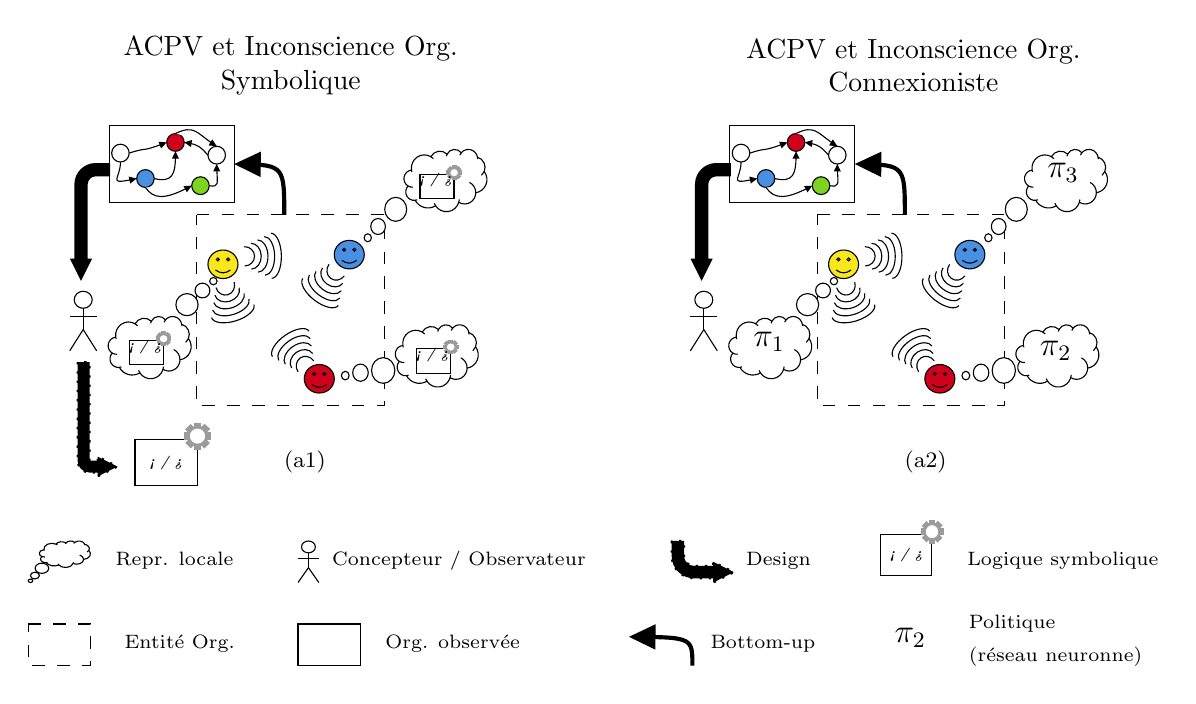
\begin{tikzpicture}[x=0.75pt,y=0.75pt,yscale=-1,xscale=1]
%uncomment if require: \path (0,1988); %set diagram left start at 0, and has height of 1988

%Shape: Rectangle [id:dp5013379967088911] 
\draw  [dash pattern={on 4.5pt off 4.5pt}] (91.18,1582.9) -- (181.55,1582.9) -- (181.55,1674.84) -- (91.18,1674.84) -- cycle ;
%Shape: Smiley Face [id:dp2909986828605782] 
\draw  [fill={rgb, 255:red, 248; green, 231; blue, 28 }  ,fill opacity=1 ] (96.6,1606.68) .. controls (96.6,1602.89) and (99.84,1599.82) .. (103.83,1599.82) .. controls (107.82,1599.82) and (111.06,1602.89) .. (111.06,1606.68) .. controls (111.06,1610.48) and (107.82,1613.55) .. (103.83,1613.55) .. controls (99.84,1613.55) and (96.6,1610.48) .. (96.6,1606.68) -- cycle ; \draw  [fill={rgb, 255:red, 248; green, 231; blue, 28 }  ,fill opacity=1 ] (100.65,1604.35) .. controls (100.65,1603.97) and (100.97,1603.66) .. (101.37,1603.66) .. controls (101.77,1603.66) and (102.09,1603.97) .. (102.09,1604.35) .. controls (102.09,1604.73) and (101.77,1605.04) .. (101.37,1605.04) .. controls (100.97,1605.04) and (100.65,1604.73) .. (100.65,1604.35) -- cycle ; \draw  [fill={rgb, 255:red, 248; green, 231; blue, 28 }  ,fill opacity=1 ] (105.56,1604.35) .. controls (105.56,1603.97) and (105.89,1603.66) .. (106.29,1603.66) .. controls (106.69,1603.66) and (107.01,1603.97) .. (107.01,1604.35) .. controls (107.01,1604.73) and (106.69,1605.04) .. (106.29,1605.04) .. controls (105.89,1605.04) and (105.56,1604.73) .. (105.56,1604.35) -- cycle ; \draw   (100.21,1609.43) .. controls (102.62,1611.26) and (105.03,1611.26) .. (107.44,1609.43) ;
%Shape: Arc [id:dp29848310914124687] 
\draw  [draw opacity=0] (118.78,1626.11) .. controls (118.78,1626.11) and (118.78,1626.11) .. (118.78,1626.11) .. controls (119.55,1628.72) and (115.59,1632.23) .. (109.94,1633.95) .. controls (104.28,1635.67) and (99.08,1634.94) .. (98.31,1632.33) -- (108.55,1629.22) -- cycle ; \draw   (118.78,1626.11) .. controls (118.78,1626.11) and (118.78,1626.11) .. (118.78,1626.11) .. controls (119.55,1628.72) and (115.59,1632.23) .. (109.94,1633.95) .. controls (104.28,1635.67) and (99.08,1634.94) .. (98.31,1632.33) ;  
%Shape: Arc [id:dp5990837957773074] 
\draw  [draw opacity=0] (116.39,1623.4) .. controls (117.16,1626.01) and (113.86,1629.32) .. (109.01,1630.8) .. controls (104.17,1632.27) and (99.62,1631.35) .. (98.85,1628.74) -- (107.62,1626.07) -- cycle ; \draw   (116.39,1623.4) .. controls (117.16,1626.01) and (113.86,1629.32) .. (109.01,1630.8) .. controls (104.17,1632.27) and (99.62,1631.35) .. (98.85,1628.74) ;  
%Shape: Arc [id:dp6042231692023955] 
\draw  [draw opacity=0] (114.01,1620.7) .. controls (114.01,1620.7) and (114.01,1620.7) .. (114.01,1620.7) .. controls (114.77,1623.31) and (112.12,1626.42) .. (108.08,1627.65) .. controls (104.05,1628.87) and (100.15,1627.75) .. (99.39,1625.14) -- (106.7,1622.92) -- cycle ; \draw   (114.01,1620.7) .. controls (114.01,1620.7) and (114.01,1620.7) .. (114.01,1620.7) .. controls (114.77,1623.31) and (112.12,1626.42) .. (108.08,1627.65) .. controls (104.05,1628.87) and (100.15,1627.75) .. (99.39,1625.14) ;  
%Shape: Arc [id:dp2913688932032118] 
\draw  [draw opacity=0] (111.62,1617.99) .. controls (111.62,1617.99) and (111.62,1617.99) .. (111.62,1617.99) .. controls (111.62,1617.99) and (111.62,1617.99) .. (111.62,1617.99) .. controls (112.39,1620.6) and (110.39,1623.51) .. (107.16,1624.49) .. controls (103.93,1625.48) and (100.69,1624.16) .. (99.92,1621.55) -- (105.77,1619.77) -- cycle ; \draw   (111.62,1617.99) .. controls (111.62,1617.99) and (111.62,1617.99) .. (111.62,1617.99) .. controls (111.62,1617.99) and (111.62,1617.99) .. (111.62,1617.99) .. controls (112.39,1620.6) and (110.39,1623.51) .. (107.16,1624.49) .. controls (103.93,1625.48) and (100.69,1624.16) .. (99.92,1621.55) ;  
%Shape: Arc [id:dp837702747005986] 
\draw  [draw opacity=0] (109.23,1615.28) .. controls (109.23,1615.28) and (109.23,1615.28) .. (109.23,1615.28) .. controls (110,1617.89) and (108.66,1620.61) .. (106.23,1621.34) .. controls (103.81,1622.08) and (101.23,1620.56) .. (100.46,1617.95) -- (104.84,1616.62) -- cycle ; \draw   (109.23,1615.28) .. controls (109.23,1615.28) and (109.23,1615.28) .. (109.23,1615.28) .. controls (110,1617.89) and (108.66,1620.61) .. (106.23,1621.34) .. controls (103.81,1622.08) and (101.23,1620.56) .. (100.46,1617.95) ;  

%Shape: Arc [id:dp942335351617398] 
\draw  [draw opacity=0] (126.91,1591.72) .. controls (126.91,1591.72) and (126.91,1591.72) .. (126.91,1591.72) .. controls (129.58,1591.67) and (131.85,1596.49) .. (131.96,1602.49) .. controls (132.08,1608.49) and (130,1613.4) .. (127.33,1613.45) -- (127.12,1602.59) -- cycle ; \draw   (126.91,1591.72) .. controls (126.91,1591.72) and (126.91,1591.72) .. (126.91,1591.72) .. controls (129.58,1591.67) and (131.85,1596.49) .. (131.96,1602.49) .. controls (132.08,1608.49) and (130,1613.4) .. (127.33,1613.45) ;  
%Shape: Arc [id:dp9374644640080091] 
\draw  [draw opacity=0] (123.7,1593.34) .. controls (126.38,1593.28) and (128.63,1597.41) .. (128.73,1602.55) .. controls (128.83,1607.7) and (126.74,1611.91) .. (124.07,1611.96) -- (123.88,1602.65) -- cycle ; \draw   (123.7,1593.34) .. controls (126.38,1593.28) and (128.63,1597.41) .. (128.73,1602.55) .. controls (128.83,1607.7) and (126.74,1611.91) .. (124.07,1611.96) ;  
%Shape: Arc [id:dp9875326017202676] 
\draw  [draw opacity=0] (120.5,1594.95) .. controls (120.5,1594.95) and (120.5,1594.95) .. (120.5,1594.95) .. controls (120.5,1594.95) and (120.5,1594.95) .. (120.5,1594.95) .. controls (123.18,1594.9) and (125.42,1598.33) .. (125.5,1602.62) .. controls (125.58,1606.9) and (123.48,1610.42) .. (120.8,1610.48) -- (120.65,1602.72) -- cycle ; \draw   (120.5,1594.95) .. controls (120.5,1594.95) and (120.5,1594.95) .. (120.5,1594.95) .. controls (120.5,1594.95) and (120.5,1594.95) .. (120.5,1594.95) .. controls (123.18,1594.9) and (125.42,1598.33) .. (125.5,1602.62) .. controls (125.58,1606.9) and (123.48,1610.42) .. (120.8,1610.48) ;  
%Shape: Arc [id:dp6395434963239012] 
\draw  [draw opacity=0] (117.3,1596.57) .. controls (119.98,1596.52) and (122.2,1599.25) .. (122.27,1602.68) .. controls (122.34,1606.11) and (120.22,1608.94) .. (117.54,1608.99) -- (117.42,1602.78) -- cycle ; \draw   (117.3,1596.57) .. controls (119.98,1596.52) and (122.2,1599.25) .. (122.27,1602.68) .. controls (122.34,1606.11) and (120.22,1608.94) .. (117.54,1608.99) ;  
%Shape: Arc [id:dp8898894473533424] 
\draw  [draw opacity=0] (114.1,1598.19) .. controls (114.1,1598.19) and (114.1,1598.19) .. (114.1,1598.19) .. controls (116.78,1598.13) and (118.99,1600.18) .. (119.04,1602.75) .. controls (119.09,1605.32) and (116.96,1607.45) .. (114.28,1607.5) -- (114.19,1602.85) -- cycle ; \draw   (114.1,1598.19) .. controls (114.1,1598.19) and (114.1,1598.19) .. (114.1,1598.19) .. controls (116.78,1598.13) and (118.99,1600.18) .. (119.04,1602.75) .. controls (119.09,1605.32) and (116.96,1607.45) .. (114.28,1607.5) ;  

%Shape: Smiley Face [id:dp7764061124552845] 
\draw  [fill={rgb, 255:red, 208; green, 2; blue, 27 }  ,fill opacity=1 ] (142.99,1661.85) .. controls (142.99,1658.05) and (146.22,1654.98) .. (150.22,1654.98) .. controls (154.21,1654.98) and (157.45,1658.05) .. (157.45,1661.85) .. controls (157.45,1665.64) and (154.21,1668.71) .. (150.22,1668.71) .. controls (146.22,1668.71) and (142.99,1665.64) .. (142.99,1661.85) -- cycle ; \draw  [fill={rgb, 255:red, 208; green, 2; blue, 27 }  ,fill opacity=1 ] (147.04,1659.51) .. controls (147.04,1659.13) and (147.36,1658.82) .. (147.76,1658.82) .. controls (148.16,1658.82) and (148.48,1659.13) .. (148.48,1659.51) .. controls (148.48,1659.89) and (148.16,1660.2) .. (147.76,1660.2) .. controls (147.36,1660.2) and (147.04,1659.89) .. (147.04,1659.51) -- cycle ; \draw  [fill={rgb, 255:red, 208; green, 2; blue, 27 }  ,fill opacity=1 ] (151.95,1659.51) .. controls (151.95,1659.13) and (152.28,1658.82) .. (152.68,1658.82) .. controls (153.07,1658.82) and (153.4,1659.13) .. (153.4,1659.51) .. controls (153.4,1659.89) and (153.07,1660.2) .. (152.68,1660.2) .. controls (152.28,1660.2) and (151.95,1659.89) .. (151.95,1659.51) -- cycle ; \draw   (146.6,1664.59) .. controls (149.01,1666.42) and (151.42,1666.42) .. (153.83,1664.59) ;
%Shape: Arc [id:dp6351137443890205] 
\draw  [draw opacity=0] (127.66,1651.18) .. controls (127.66,1651.18) and (127.66,1651.18) .. (127.66,1651.18) .. controls (126.14,1648.93) and (128.86,1644.36) .. (133.72,1640.96) .. controls (138.59,1637.57) and (143.76,1636.64) .. (145.28,1638.88) -- (136.47,1645.03) -- cycle ; \draw   (127.66,1651.18) .. controls (127.66,1651.18) and (127.66,1651.18) .. (127.66,1651.18) .. controls (126.14,1648.93) and (128.86,1644.36) .. (133.72,1640.96) .. controls (138.59,1637.57) and (143.76,1636.64) .. (145.28,1638.88) ;  
%Shape: Arc [id:dp14384542342253448] 
\draw  [draw opacity=0] (130.74,1653.01) .. controls (130.74,1653.01) and (130.74,1653.01) .. (130.74,1653.01) .. controls (129.23,1650.76) and (131.38,1646.58) .. (135.55,1643.67) .. controls (139.72,1640.76) and (144.33,1640.23) .. (145.85,1642.47) -- (138.29,1647.74) -- cycle ; \draw   (130.74,1653.01) .. controls (130.74,1653.01) and (130.74,1653.01) .. (130.74,1653.01) .. controls (129.23,1650.76) and (131.38,1646.58) .. (135.55,1643.67) .. controls (139.72,1640.76) and (144.33,1640.23) .. (145.85,1642.47) ;  
%Shape: Arc [id:dp5122941757438816] 
\draw  [draw opacity=0] (133.83,1654.84) .. controls (132.32,1652.6) and (133.91,1648.81) .. (137.38,1646.39) .. controls (140.86,1643.96) and (144.9,1643.82) .. (146.42,1646.06) -- (140.12,1650.45) -- cycle ; \draw   (133.83,1654.84) .. controls (132.32,1652.6) and (133.91,1648.81) .. (137.38,1646.39) .. controls (140.86,1643.96) and (144.9,1643.82) .. (146.42,1646.06) ;  
%Shape: Arc [id:dp07424291454569965] 
\draw  [draw opacity=0] (136.92,1656.68) .. controls (136.92,1656.68) and (136.92,1656.68) .. (136.92,1656.68) .. controls (135.4,1654.43) and (136.43,1651.04) .. (139.21,1649.1) .. controls (141.99,1647.16) and (145.47,1647.41) .. (146.99,1649.65) -- (141.95,1653.17) -- cycle ; \draw   (136.92,1656.68) .. controls (136.92,1656.68) and (136.92,1656.68) .. (136.92,1656.68) .. controls (135.4,1654.43) and (136.43,1651.04) .. (139.21,1649.1) .. controls (141.99,1647.16) and (145.47,1647.41) .. (146.99,1649.65) ;  
%Shape: Arc [id:dp21630199602073374] 
\draw  [draw opacity=0] (140,1658.51) .. controls (140,1658.51) and (140,1658.51) .. (140,1658.51) .. controls (138.49,1656.27) and (138.95,1653.26) .. (141.04,1651.81) .. controls (143.12,1650.36) and (146.04,1651) .. (147.55,1653.24) -- (143.78,1655.88) -- cycle ; \draw   (140,1658.51) .. controls (140,1658.51) and (140,1658.51) .. (140,1658.51) .. controls (138.49,1656.27) and (138.95,1653.26) .. (141.04,1651.81) .. controls (143.12,1650.36) and (146.04,1651) .. (147.55,1653.24) ;  

%Shape: Smiley Face [id:dp08426871234533728] 
\draw  [fill={rgb, 255:red, 74; green, 144; blue, 226 }  ,fill opacity=1 ] (157.45,1602.03) .. controls (157.45,1598.23) and (160.68,1595.16) .. (164.68,1595.16) .. controls (168.67,1595.16) and (171.91,1598.23) .. (171.91,1602.03) .. controls (171.91,1605.82) and (168.67,1608.89) .. (164.68,1608.89) .. controls (160.68,1608.89) and (157.45,1605.82) .. (157.45,1602.03) -- cycle ; \draw  [fill={rgb, 255:red, 74; green, 144; blue, 226 }  ,fill opacity=1 ] (161.5,1599.69) .. controls (161.5,1599.31) and (161.82,1599.01) .. (162.22,1599.01) .. controls (162.62,1599.01) and (162.94,1599.31) .. (162.94,1599.69) .. controls (162.94,1600.07) and (162.62,1600.38) .. (162.22,1600.38) .. controls (161.82,1600.38) and (161.5,1600.07) .. (161.5,1599.69) -- cycle ; \draw  [fill={rgb, 255:red, 74; green, 144; blue, 226 }  ,fill opacity=1 ] (166.41,1599.69) .. controls (166.41,1599.31) and (166.74,1599.01) .. (167.13,1599.01) .. controls (167.53,1599.01) and (167.86,1599.31) .. (167.86,1599.69) .. controls (167.86,1600.07) and (167.53,1600.38) .. (167.13,1600.38) .. controls (166.74,1600.38) and (166.41,1600.07) .. (166.41,1599.69) -- cycle ; \draw   (161.06,1604.77) .. controls (163.47,1606.6) and (165.88,1606.6) .. (168.29,1604.77) ;
%Shape: Arc [id:dp02754459389784214] 
\draw  [draw opacity=0] (159.38,1626.55) .. controls (159.38,1626.55) and (159.38,1626.55) .. (159.38,1626.55) .. controls (157.77,1628.72) and (152.64,1627.57) .. (147.92,1623.98) .. controls (143.2,1620.38) and (140.68,1615.69) .. (142.28,1613.51) -- (150.83,1620.03) -- cycle ; \draw   (159.38,1626.55) .. controls (159.38,1626.55) and (159.38,1626.55) .. (159.38,1626.55) .. controls (157.77,1628.72) and (152.64,1627.57) .. (147.92,1623.98) .. controls (143.2,1620.38) and (140.68,1615.69) .. (142.28,1613.51) ;  
%Shape: Arc [id:dp8443099266344009] 
\draw  [draw opacity=0] (160.1,1622.98) .. controls (160.1,1622.98) and (160.1,1622.98) .. (160.1,1622.98) .. controls (160.1,1622.98) and (160.1,1622.98) .. (160.1,1622.98) .. controls (158.49,1625.16) and (153.91,1624.43) .. (149.86,1621.34) .. controls (145.81,1618.26) and (143.84,1613.99) .. (145.44,1611.81) -- (152.77,1617.4) -- cycle ; \draw   (160.1,1622.98) .. controls (160.1,1622.98) and (160.1,1622.98) .. (160.1,1622.98) .. controls (160.1,1622.98) and (160.1,1622.98) .. (160.1,1622.98) .. controls (158.49,1625.16) and (153.91,1624.43) .. (149.86,1621.34) .. controls (145.81,1618.26) and (143.84,1613.99) .. (145.44,1611.81) ;  
%Shape: Arc [id:dp36090403949084215] 
\draw  [draw opacity=0] (160.81,1619.42) .. controls (159.21,1621.6) and (155.17,1621.28) .. (151.8,1618.71) .. controls (148.43,1616.14) and (146.99,1612.29) .. (148.6,1610.11) -- (154.71,1614.77) -- cycle ; \draw   (160.81,1619.42) .. controls (159.21,1621.6) and (155.17,1621.28) .. (151.8,1618.71) .. controls (148.43,1616.14) and (146.99,1612.29) .. (148.6,1610.11) ;  
%Shape: Arc [id:dp8389598515474829] 
\draw  [draw opacity=0] (161.53,1615.86) .. controls (161.53,1615.86) and (161.53,1615.86) .. (161.53,1615.86) .. controls (159.92,1618.04) and (156.44,1618.14) .. (153.74,1616.08) .. controls (151.04,1614.02) and (150.15,1610.59) .. (151.76,1608.41) -- (156.65,1612.13) -- cycle ; \draw   (161.53,1615.86) .. controls (161.53,1615.86) and (161.53,1615.86) .. (161.53,1615.86) .. controls (159.92,1618.04) and (156.44,1618.14) .. (153.74,1616.08) .. controls (151.04,1614.02) and (150.15,1610.59) .. (151.76,1608.41) ;  
%Shape: Arc [id:dp45749711978150187] 
\draw  [draw opacity=0] (162.25,1612.29) .. controls (162.25,1612.29) and (162.25,1612.29) .. (162.25,1612.29) .. controls (162.25,1612.29) and (162.25,1612.29) .. (162.25,1612.29) .. controls (160.64,1614.47) and (157.7,1614.99) .. (155.68,1613.45) .. controls (153.65,1611.91) and (153.31,1608.89) .. (154.92,1606.71) -- (158.58,1609.5) -- cycle ; \draw   (162.25,1612.29) .. controls (162.25,1612.29) and (162.25,1612.29) .. (162.25,1612.29) .. controls (162.25,1612.29) and (162.25,1612.29) .. (162.25,1612.29) .. controls (160.64,1614.47) and (157.7,1614.99) .. (155.68,1613.45) .. controls (153.65,1611.91) and (153.31,1608.89) .. (154.92,1606.71) ;  

%Shape: Rectangle [id:dp7060287107715945] 
\draw  [fill={rgb, 255:red, 255; green, 255; blue, 255 }  ,fill opacity=1 ] (49,1540) -- (109.25,1540) -- (109.25,1576.77) -- (49,1576.77) -- cycle ;
%Shape: Ellipse [id:dp8204500766763589] 
\draw  [fill={rgb, 255:red, 255; green, 255; blue, 255 }  ,fill opacity=1 ] (50.21,1553.12) .. controls (50.21,1550.75) and (52.1,1548.83) .. (54.43,1548.83) .. controls (56.76,1548.83) and (58.64,1550.75) .. (58.64,1553.12) .. controls (58.64,1555.49) and (56.76,1557.41) .. (54.43,1557.41) .. controls (52.1,1557.41) and (50.21,1555.49) .. (50.21,1553.12) -- cycle ;
%Shape: Ellipse [id:dp5181525806308303] 
\draw  [fill={rgb, 255:red, 74; green, 144; blue, 226 }  ,fill opacity=1 ] (62.26,1565.37) .. controls (62.26,1563) and (64.15,1561.08) .. (66.48,1561.08) .. controls (68.81,1561.08) and (70.69,1563) .. (70.69,1565.37) .. controls (70.69,1567.74) and (68.81,1569.66) .. (66.48,1569.66) .. controls (64.15,1569.66) and (62.26,1567.74) .. (62.26,1565.37) -- cycle ;
%Shape: Ellipse [id:dp0906893320423029] 
\draw  [fill={rgb, 255:red, 208; green, 2; blue, 27 }  ,fill opacity=1 ] (76.72,1547.97) .. controls (76.72,1545.6) and (78.61,1543.68) .. (80.94,1543.68) .. controls (83.26,1543.68) and (85.15,1545.6) .. (85.15,1547.97) .. controls (85.15,1550.34) and (83.26,1552.26) .. (80.94,1552.26) .. controls (78.61,1552.26) and (76.72,1550.34) .. (76.72,1547.97) -- cycle ;
%Shape: Ellipse [id:dp3404459677220828] 
\draw  [fill={rgb, 255:red, 255; green, 255; blue, 255 }  ,fill opacity=1 ] (96.6,1554.1) .. controls (96.6,1551.73) and (98.49,1549.81) .. (100.82,1549.81) .. controls (103.15,1549.81) and (105.03,1551.73) .. (105.03,1554.1) .. controls (105.03,1556.47) and (103.15,1558.39) .. (100.82,1558.39) .. controls (98.49,1558.39) and (96.6,1556.47) .. (96.6,1554.1) -- cycle ;
%Shape: Ellipse [id:dp7841877382320065] 
\draw  [fill={rgb, 255:red, 126; green, 211; blue, 33 }  ,fill opacity=1 ] (88.77,1568.81) .. controls (88.77,1566.44) and (90.66,1564.52) .. (92.98,1564.52) .. controls (95.31,1564.52) and (97.2,1566.44) .. (97.2,1568.81) .. controls (97.2,1571.18) and (95.31,1573.1) .. (92.98,1573.1) .. controls (90.66,1573.1) and (88.77,1571.18) .. (88.77,1568.81) -- cycle ;
%Curve Lines [id:da8931114055545611] 
\draw [fill={rgb, 255:red, 255; green, 255; blue, 255 }  ,fill opacity=1 ]   (58.64,1553.12) .. controls (68.12,1550.05) and (63.67,1552.76) .. (73.92,1549.01) ;
\draw [shift={(76.72,1547.97)}, rotate = 159.17] [fill={rgb, 255:red, 0; green, 0; blue, 0 }  ][line width=0.08]  [draw opacity=0] (3.57,-1.72) -- (0,0) -- (3.57,1.72) -- cycle    ;
%Curve Lines [id:da7735282082131947] 
\draw [fill={rgb, 255:red, 255; green, 255; blue, 255 }  ,fill opacity=1 ]   (70.69,1565.37) .. controls (79.76,1567.65) and (80.8,1562.63) .. (80.92,1555.25) ;
\draw [shift={(80.94,1552.26)}, rotate = 90] [fill={rgb, 255:red, 0; green, 0; blue, 0 }  ][line width=0.08]  [draw opacity=0] (3.57,-1.72) -- (0,0) -- (3.57,1.72) -- cycle    ;
%Curve Lines [id:da8607237334353054] 
\draw [fill={rgb, 255:red, 255; green, 255; blue, 255 }  ,fill opacity=1 ]   (96.6,1554.1) .. controls (93.1,1550.33) and (92.09,1549.27) .. (88.06,1548.46) ;
\draw [shift={(85.15,1547.97)}, rotate = 8.42] [fill={rgb, 255:red, 0; green, 0; blue, 0 }  ][line width=0.08]  [draw opacity=0] (3.57,-1.72) -- (0,0) -- (3.57,1.72) -- cycle    ;
%Curve Lines [id:da39004498418287703] 
\draw [fill={rgb, 255:red, 255; green, 255; blue, 255 }  ,fill opacity=1 ]   (97.2,1568.81) .. controls (101.97,1569.67) and (101.15,1567.87) .. (100.88,1561.33) ;
\draw [shift={(100.82,1558.39)}, rotate = 90] [fill={rgb, 255:red, 0; green, 0; blue, 0 }  ][line width=0.08]  [draw opacity=0] (3.57,-1.72) -- (0,0) -- (3.57,1.72) -- cycle    ;
%Curve Lines [id:da9723906849673678] 
\draw [fill={rgb, 255:red, 255; green, 255; blue, 255 }  ,fill opacity=1 ]   (54.43,1557.41) .. controls (54.43,1565.5) and (48.17,1568.19) .. (59.41,1565.96) ;
\draw [shift={(62.26,1565.37)}, rotate = 168.05] [fill={rgb, 255:red, 0; green, 0; blue, 0 }  ][line width=0.08]  [draw opacity=0] (3.57,-1.72) -- (0,0) -- (3.57,1.72) -- cycle    ;
%Curve Lines [id:da2389978943863197] 
\draw [fill={rgb, 255:red, 255; green, 255; blue, 255 }  ,fill opacity=1 ]   (66.48,1569.66) .. controls (70.38,1575.45) and (75.82,1575.36) .. (86.16,1570.17) ;
\draw [shift={(88.77,1568.81)}, rotate = 151.67] [fill={rgb, 255:red, 0; green, 0; blue, 0 }  ][line width=0.08]  [draw opacity=0] (3.57,-1.72) -- (0,0) -- (3.57,1.72) -- cycle    ;
%Curve Lines [id:da9606608376740503] 
\draw [fill={rgb, 255:red, 255; green, 255; blue, 255 }  ,fill opacity=1 ]   (80.94,1543.68) .. controls (89.71,1539.44) and (91,1543.12) .. (98.42,1548.25) ;
\draw [shift={(100.82,1549.81)}, rotate = 211.4] [fill={rgb, 255:red, 0; green, 0; blue, 0 }  ][line width=0.08]  [draw opacity=0] (3.57,-1.72) -- (0,0) -- (3.57,1.72) -- cycle    ;
%Shape: Ellipse [id:dp8238624688148318] 
\draw   (32.16,1623.78) .. controls (32.16,1621.51) and (34.1,1619.68) .. (36.49,1619.68) .. controls (38.88,1619.68) and (40.82,1621.51) .. (40.82,1623.78) .. controls (40.82,1626.04) and (38.88,1627.88) .. (36.49,1627.88) .. controls (34.1,1627.88) and (32.16,1626.04) .. (32.16,1623.78) -- cycle ;
%Straight Lines [id:da1506125445454658] 
\draw    (36.49,1627.88) -- (36.49,1638.12) ;
%Straight Lines [id:da49468464160952785] 
\draw    (36.49,1638.12) -- (30,1648.37) ;
%Straight Lines [id:da131299671574843] 
\draw    (36.49,1638.12) -- (42.98,1648.37) ;
%Straight Lines [id:da7804526802882297] 
\draw    (42.98,1631.98) -- (30,1631.98) ;

%Bend Arrow [id:dp6575031643828187] 
\draw  [fill={rgb, 255:red, 0; green, 0; blue, 0 }  ,fill opacity=1 ][line width=0.75]  (49,1558.39) -- (42.5,1558.39) .. controls (37.11,1558.39) and (32.74,1562.76) .. (32.74,1568.15) -- (32.74,1604.51) -- (30.93,1604.51) -- (35.45,1613.55) -- (39.97,1604.51) -- (38.16,1604.51) -- (38.16,1568.15) .. controls (38.16,1565.75) and (40.1,1563.81) .. (42.5,1563.81) -- (49,1563.81) -- cycle ;
%Shape: Boxed Bezier Curve [id:dp6472304808727206] 
\draw [line width=1.5]    (133.35,1582.9) .. controls (133.35,1559.97) and (133.35,1558.71) .. (113.01,1558.43) ;
\draw [shift={(109.25,1558.39)}, rotate = 0.58] [fill={rgb, 255:red, 0; green, 0; blue, 0 }  ][line width=0.08]  [draw opacity=0] (12.77,-6.13) -- (0,0) -- (12.77,6.13) -- cycle    ;

%Shape: Cloud [id:dp9267969156542857] 
\draw  [fill={rgb, 255:red, 255; green, 255; blue, 255 }  ,fill opacity=1 ] (52.14,1641.72) .. controls (51.82,1639.3) and (52.88,1636.9) .. (54.86,1635.55) .. controls (56.85,1634.19) and (59.42,1634.12) .. (61.48,1635.35) .. controls (62.21,1633.95) and (63.55,1632.97) .. (65.09,1632.73) .. controls (66.63,1632.49) and (68.19,1633.01) .. (69.3,1634.12) .. controls (69.92,1632.85) and (71.14,1631.99) .. (72.53,1631.86) .. controls (73.92,1631.72) and (75.28,1632.33) .. (76.12,1633.46) .. controls (77.24,1632.11) and (79.03,1631.54) .. (80.71,1632) .. controls (82.39,1632.46) and (83.66,1633.87) .. (83.97,1635.61) .. controls (85.34,1636) and (86.49,1636.97) .. (87.11,1638.29) .. controls (87.73,1639.6) and (87.77,1641.13) .. (87.2,1642.47) .. controls (88.56,1644.28) and (88.88,1646.68) .. (88.04,1648.79) .. controls (87.2,1650.89) and (85.33,1652.38) .. (83.12,1652.71) .. controls (83.11,1654.68) and (82.05,1656.5) .. (80.35,1657.45) .. controls (78.65,1658.4) and (76.58,1658.34) .. (74.94,1657.3) .. controls (74.24,1659.66) and (72.27,1661.41) .. (69.88,1661.77) .. controls (67.49,1662.13) and (65.12,1661.05) .. (63.77,1659) .. controls (62.13,1660.01) and (60.15,1660.3) .. (58.3,1659.81) .. controls (56.44,1659.31) and (54.86,1658.07) .. (53.9,1656.36) .. controls (52.22,1656.56) and (50.6,1655.67) .. (49.83,1654.13) .. controls (49.07,1652.6) and (49.33,1650.73) .. (50.49,1649.48) .. controls (48.99,1648.57) and (48.22,1646.78) .. (48.59,1645.04) .. controls (48.96,1643.3) and (50.38,1641.99) .. (52.11,1641.81) ; \draw   (50.49,1649.48) .. controls (51.2,1649.9) and (52.01,1650.09) .. (52.83,1650.03)(53.9,1656.36) .. controls (54.25,1656.32) and (54.6,1656.23) .. (54.93,1656.1)(63.77,1659) .. controls (63.53,1658.62) and (63.32,1658.21) .. (63.16,1657.79)(74.94,1657.3) .. controls (75.07,1656.86) and (75.15,1656.42) .. (75.19,1655.97)(83.12,1652.71) .. controls (83.14,1650.6) and (81.97,1648.68) .. (80.11,1647.75)(87.2,1642.47) .. controls (86.9,1643.19) and (86.44,1643.82) .. (85.86,1644.33)(83.97,1635.61) .. controls (84.02,1635.9) and (84.04,1636.19) .. (84.04,1636.49)(76.12,1633.46) .. controls (75.84,1633.8) and (75.61,1634.18) .. (75.43,1634.58)(69.3,1634.12) .. controls (69.15,1634.43) and (69.04,1634.75) .. (68.97,1635.09)(61.48,1635.35) .. controls (61.92,1635.61) and (62.32,1635.93) .. (62.69,1636.29)(52.14,1641.72) .. controls (52.18,1642.05) and (52.25,1642.38) .. (52.35,1642.7) ;
%Shape: Cloud [id:dp5528798724302991] 
\draw  [fill={rgb, 255:red, 255; green, 255; blue, 255 }  ,fill opacity=1 ] (194.64,1561.22) .. controls (194.32,1558.8) and (195.38,1556.4) .. (197.36,1555.05) .. controls (199.35,1553.69) and (201.92,1553.62) .. (203.98,1554.85) .. controls (204.71,1553.45) and (206.05,1552.47) .. (207.59,1552.23) .. controls (209.13,1551.99) and (210.69,1552.51) .. (211.8,1553.62) .. controls (212.42,1552.35) and (213.64,1551.49) .. (215.03,1551.36) .. controls (216.42,1551.22) and (217.78,1551.83) .. (218.62,1552.96) .. controls (219.74,1551.61) and (221.53,1551.04) .. (223.21,1551.5) .. controls (224.89,1551.96) and (226.16,1553.37) .. (226.47,1555.11) .. controls (227.84,1555.5) and (228.99,1556.47) .. (229.61,1557.79) .. controls (230.23,1559.1) and (230.27,1560.63) .. (229.7,1561.97) .. controls (231.06,1563.78) and (231.38,1566.18) .. (230.54,1568.29) .. controls (229.7,1570.39) and (227.83,1571.88) .. (225.62,1572.21) .. controls (225.61,1574.18) and (224.55,1576) .. (222.85,1576.95) .. controls (221.15,1577.9) and (219.08,1577.84) .. (217.44,1576.8) .. controls (216.74,1579.16) and (214.77,1580.91) .. (212.38,1581.27) .. controls (209.99,1581.63) and (207.62,1580.55) .. (206.27,1578.5) .. controls (204.63,1579.51) and (202.65,1579.8) .. (200.8,1579.31) .. controls (198.94,1578.81) and (197.36,1577.57) .. (196.4,1575.86) .. controls (194.72,1576.06) and (193.1,1575.17) .. (192.33,1573.63) .. controls (191.57,1572.1) and (191.83,1570.23) .. (192.99,1568.98) .. controls (191.49,1568.07) and (190.72,1566.28) .. (191.09,1564.54) .. controls (191.46,1562.8) and (192.88,1561.49) .. (194.61,1561.31) ; \draw   (192.99,1568.98) .. controls (193.7,1569.4) and (194.51,1569.59) .. (195.33,1569.53)(196.4,1575.86) .. controls (196.75,1575.82) and (197.1,1575.73) .. (197.43,1575.6)(206.27,1578.5) .. controls (206.03,1578.12) and (205.82,1577.71) .. (205.66,1577.29)(217.44,1576.8) .. controls (217.57,1576.36) and (217.65,1575.92) .. (217.69,1575.47)(225.62,1572.21) .. controls (225.64,1570.1) and (224.47,1568.18) .. (222.61,1567.25)(229.7,1561.97) .. controls (229.4,1562.69) and (228.94,1563.32) .. (228.36,1563.83)(226.47,1555.11) .. controls (226.52,1555.4) and (226.54,1555.69) .. (226.54,1555.99)(218.62,1552.96) .. controls (218.34,1553.3) and (218.11,1553.68) .. (217.93,1554.08)(211.8,1553.62) .. controls (211.65,1553.93) and (211.54,1554.25) .. (211.47,1554.59)(203.98,1554.85) .. controls (204.42,1555.11) and (204.82,1555.43) .. (205.19,1555.79)(194.64,1561.22) .. controls (194.68,1561.55) and (194.75,1561.88) .. (194.85,1562.2) ;
%Shape: Ellipse [id:dp7514204534640926] 
\draw  [fill={rgb, 255:red, 255; green, 255; blue, 255 }  ,fill opacity=1 ] (175.03,1588.48) .. controls (175.03,1586.36) and (176.61,1584.63) .. (178.56,1584.63) .. controls (180.51,1584.63) and (182.09,1586.36) .. (182.09,1588.48) .. controls (182.09,1590.6) and (180.51,1592.33) .. (178.56,1592.33) .. controls (176.61,1592.33) and (175.03,1590.6) .. (175.03,1588.48) -- cycle ;
%Shape: Ellipse [id:dp44553318612962955] 
\draw  [fill={rgb, 255:red, 255; green, 255; blue, 255 }  ,fill opacity=1 ] (171.83,1593.92) .. controls (171.83,1592.85) and (172.62,1591.99) .. (173.6,1591.99) .. controls (174.57,1591.99) and (175.36,1592.85) .. (175.36,1593.92) .. controls (175.36,1594.98) and (174.57,1595.84) .. (173.6,1595.84) .. controls (172.62,1595.84) and (171.83,1594.98) .. (171.83,1593.92) -- cycle ;
%Shape: Ellipse [id:dp82913236602551] 
\draw  [fill={rgb, 255:red, 255; green, 255; blue, 255 }  ,fill opacity=1 ] (90.37,1619.32) .. controls (90.37,1617.36) and (91.97,1615.77) .. (93.94,1615.77) .. controls (95.91,1615.77) and (97.51,1617.36) .. (97.51,1619.32) .. controls (97.51,1621.28) and (95.91,1622.87) .. (93.94,1622.87) .. controls (91.97,1622.87) and (90.37,1621.28) .. (90.37,1619.32) -- cycle ;
%Shape: Ellipse [id:dp2375828747719494] 
\draw  [fill={rgb, 255:red, 255; green, 255; blue, 255 }  ,fill opacity=1 ] (81.14,1626.14) .. controls (81.14,1623.2) and (83.53,1620.81) .. (86.49,1620.81) .. controls (89.44,1620.81) and (91.84,1623.2) .. (91.84,1626.14) .. controls (91.84,1629.08) and (89.44,1631.46) .. (86.49,1631.46) .. controls (83.53,1631.46) and (81.14,1629.08) .. (81.14,1626.14) -- cycle ;
%Shape: Ellipse [id:dp42236739615338126] 
\draw  [fill={rgb, 255:red, 255; green, 255; blue, 255 }  ,fill opacity=1 ] (97.42,1614.8) .. controls (97.42,1613.82) and (98.22,1613.02) .. (99.2,1613.02) .. controls (100.19,1613.02) and (100.98,1613.82) .. (100.98,1614.8) .. controls (100.98,1615.78) and (100.19,1616.57) .. (99.2,1616.57) .. controls (98.22,1616.57) and (97.42,1615.78) .. (97.42,1614.8) -- cycle ;
%Shape: Ellipse [id:dp9447534834781316] 
\draw  [fill={rgb, 255:red, 255; green, 255; blue, 255 }  ,fill opacity=1 ] (181.75,1580.2) .. controls (181.75,1577.01) and (184.13,1574.43) .. (187.05,1574.43) .. controls (189.97,1574.43) and (192.34,1577.01) .. (192.34,1580.2) .. controls (192.34,1583.38) and (189.97,1585.97) .. (187.05,1585.97) .. controls (184.13,1585.97) and (181.75,1583.38) .. (181.75,1580.2) -- cycle ;
%Shape: Ellipse [id:dp5194641468129697] 
\draw  [fill={rgb, 255:red, 255; green, 255; blue, 255 }  ,fill opacity=1 ] (175.41,1657.84) .. controls (175.41,1654.42) and (177.93,1651.65) .. (181.03,1651.65) .. controls (184.12,1651.65) and (186.64,1654.42) .. (186.64,1657.84) .. controls (186.64,1661.26) and (184.12,1664.03) .. (181.03,1664.03) .. controls (177.93,1664.03) and (175.41,1661.26) .. (175.41,1657.84) -- cycle ;
%Shape: Ellipse [id:dp7757831456715724] 
\draw  [fill={rgb, 255:red, 255; green, 255; blue, 255 }  ,fill opacity=1 ] (166.34,1658.91) .. controls (166.34,1656.63) and (168.02,1654.78) .. (170.08,1654.78) .. controls (172.15,1654.78) and (173.82,1656.63) .. (173.82,1658.91) .. controls (173.82,1661.19) and (172.15,1663.04) .. (170.08,1663.04) .. controls (168.02,1663.04) and (166.34,1661.19) .. (166.34,1658.91) -- cycle ;
%Shape: Ellipse [id:dp29373407797568707] 
\draw  [fill={rgb, 255:red, 255; green, 255; blue, 255 }  ,fill opacity=1 ] (160.88,1660.31) .. controls (160.88,1659.17) and (161.72,1658.25) .. (162.75,1658.25) .. controls (163.78,1658.25) and (164.62,1659.17) .. (164.62,1660.31) .. controls (164.62,1661.45) and (163.78,1662.38) .. (162.75,1662.38) .. controls (161.72,1662.38) and (160.88,1661.45) .. (160.88,1660.31) -- cycle ;
%Flowchart: Process [id:dp9834032610152076] 
\draw   (58.74,1643.45) -- (75.11,1643.45) -- (75.11,1655.13) -- (58.74,1655.13) -- cycle ;
%Shape: Ellipse [id:dp6640670880210211] 
\draw  [color={rgb, 255:red, 155; green, 155; blue, 155 }  ,draw opacity=1 ][fill={rgb, 255:red, 155; green, 155; blue, 155 }  ,fill opacity=1 ] (72.58,1642.54) .. controls (72.58,1641.17) and (73.76,1640.07) .. (75.22,1640.07) .. controls (76.68,1640.07) and (77.86,1641.17) .. (77.86,1642.54) .. controls (77.86,1643.91) and (76.68,1645.01) .. (75.22,1645.01) .. controls (73.76,1645.01) and (72.58,1643.91) .. (72.58,1642.54) -- cycle ;
%Shape: Rectangle [id:dp5232643763802065] 
\draw  [color={rgb, 255:red, 155; green, 155; blue, 155 }  ,draw opacity=1 ][fill={rgb, 255:red, 155; green, 155; blue, 155 }  ,fill opacity=1 ] (74.34,1639.24) -- (76.1,1639.24) -- (76.1,1640.89) -- (74.34,1640.89) -- cycle ;
%Shape: Rectangle [id:dp9098850223722781] 
\draw  [color={rgb, 255:red, 155; green, 155; blue, 155 }  ,draw opacity=1 ][fill={rgb, 255:red, 155; green, 155; blue, 155 }  ,fill opacity=1 ] (76.98,1641.72) -- (78.74,1641.72) -- (78.74,1643.36) -- (76.98,1643.36) -- cycle ;
%Shape: Rectangle [id:dp27460898986906623] 
\draw  [color={rgb, 255:red, 155; green, 155; blue, 155 }  ,draw opacity=1 ][fill={rgb, 255:red, 155; green, 155; blue, 155 }  ,fill opacity=1 ] (74.34,1644.19) -- (76.1,1644.19) -- (76.1,1645.84) -- (74.34,1645.84) -- cycle ;
%Shape: Rectangle [id:dp42946228539873565] 
\draw  [color={rgb, 255:red, 155; green, 155; blue, 155 }  ,draw opacity=1 ][fill={rgb, 255:red, 155; green, 155; blue, 155 }  ,fill opacity=1 ] (71.7,1641.72) -- (73.46,1641.72) -- (73.46,1643.36) -- (71.7,1643.36) -- cycle ;
%Shape: Rectangle [id:dp7904848912164214] 
\draw  [color={rgb, 255:red, 155; green, 155; blue, 155 }  ,draw opacity=1 ][fill={rgb, 255:red, 155; green, 155; blue, 155 }  ,fill opacity=1 ] (73.42,1639.69) -- (74.66,1640.86) -- (73.42,1642.02) -- (72.17,1640.86) -- cycle ;
%Shape: Rectangle [id:dp3301141202355372] 
\draw  [color={rgb, 255:red, 155; green, 155; blue, 155 }  ,draw opacity=1 ][fill={rgb, 255:red, 155; green, 155; blue, 155 }  ,fill opacity=1 ] (77.04,1643.12) -- (78.28,1644.29) -- (77.04,1645.45) -- (75.8,1644.29) -- cycle ;
%Shape: Rectangle [id:dp6342375560239414] 
\draw  [color={rgb, 255:red, 155; green, 155; blue, 155 }  ,draw opacity=1 ][fill={rgb, 255:red, 155; green, 155; blue, 155 }  ,fill opacity=1 ] (73.45,1643.09) -- (74.69,1644.26) -- (73.45,1645.42) -- (72.21,1644.26) -- cycle ;
%Shape: Rectangle [id:dp3754059778400457] 
\draw  [color={rgb, 255:red, 155; green, 155; blue, 155 }  ,draw opacity=1 ][fill={rgb, 255:red, 155; green, 155; blue, 155 }  ,fill opacity=1 ] (77.1,1639.59) -- (78.34,1640.76) -- (77.1,1641.93) -- (75.86,1640.76) -- cycle ;
%Shape: Ellipse [id:dp7736710329933231] 
\draw  [color={rgb, 255:red, 155; green, 155; blue, 155 }  ,draw opacity=1 ][fill={rgb, 255:red, 255; green, 255; blue, 255 }  ,fill opacity=1 ] (73.02,1642.54) .. controls (73.02,1641.4) and (74.01,1640.48) .. (75.22,1640.48) .. controls (76.44,1640.48) and (77.42,1641.4) .. (77.42,1642.54) .. controls (77.42,1643.68) and (76.44,1644.6) .. (75.22,1644.6) .. controls (74.01,1644.6) and (73.02,1643.68) .. (73.02,1642.54) -- cycle ;

%Shape: Cloud [id:dp8515242927252613] 
\draw  [fill={rgb, 255:red, 255; green, 255; blue, 255 }  ,fill opacity=1 ] (190.48,1645.72) .. controls (190.15,1643.3) and (191.21,1640.9) .. (193.2,1639.55) .. controls (195.19,1638.19) and (197.76,1638.12) .. (199.82,1639.35) .. controls (200.55,1637.95) and (201.89,1636.97) .. (203.43,1636.73) .. controls (204.97,1636.49) and (206.53,1637.01) .. (207.64,1638.12) .. controls (208.26,1636.85) and (209.48,1635.99) .. (210.87,1635.86) .. controls (212.25,1635.72) and (213.61,1636.33) .. (214.46,1637.46) .. controls (215.58,1636.11) and (217.37,1635.54) .. (219.05,1636) .. controls (220.73,1636.46) and (221.99,1637.87) .. (222.3,1639.61) .. controls (223.68,1640) and (224.83,1640.97) .. (225.45,1642.29) .. controls (226.07,1643.6) and (226.1,1645.13) .. (225.54,1646.47) .. controls (226.9,1648.28) and (227.21,1650.68) .. (226.37,1652.79) .. controls (225.53,1654.89) and (223.66,1656.38) .. (221.46,1656.71) .. controls (221.44,1658.68) and (220.38,1660.5) .. (218.68,1661.45) .. controls (216.99,1662.4) and (214.92,1662.34) .. (213.28,1661.3) .. controls (212.58,1663.66) and (210.61,1665.41) .. (208.22,1665.77) .. controls (205.83,1666.13) and (203.45,1665.05) .. (202.11,1663) .. controls (200.46,1664.01) and (198.49,1664.3) .. (196.63,1663.81) .. controls (194.78,1663.31) and (193.19,1662.07) .. (192.24,1660.36) .. controls (190.56,1660.56) and (188.93,1659.67) .. (188.17,1658.13) .. controls (187.41,1656.6) and (187.67,1654.73) .. (188.82,1653.48) .. controls (187.32,1652.57) and (186.56,1650.78) .. (186.93,1649.04) .. controls (187.3,1647.3) and (188.71,1645.99) .. (190.44,1645.81) ; \draw   (188.82,1653.48) .. controls (189.53,1653.9) and (190.35,1654.09) .. (191.17,1654.03)(192.24,1660.36) .. controls (192.59,1660.32) and (192.93,1660.23) .. (193.26,1660.1)(202.11,1663) .. controls (201.86,1662.62) and (201.65,1662.21) .. (201.49,1661.79)(213.28,1661.3) .. controls (213.4,1660.86) and (213.49,1660.42) .. (213.52,1659.97)(221.46,1656.71) .. controls (221.47,1654.6) and (220.3,1652.68) .. (218.45,1651.75)(225.54,1646.47) .. controls (225.24,1647.19) and (224.78,1647.82) .. (224.2,1648.33)(222.3,1639.61) .. controls (222.35,1639.9) and (222.38,1640.19) .. (222.37,1640.49)(214.46,1637.46) .. controls (214.18,1637.8) and (213.95,1638.18) .. (213.77,1638.58)(207.64,1638.12) .. controls (207.49,1638.43) and (207.37,1638.75) .. (207.3,1639.09)(199.82,1639.35) .. controls (200.26,1639.61) and (200.66,1639.93) .. (201.02,1640.29)(190.48,1645.72) .. controls (190.52,1646.05) and (190.59,1646.38) .. (190.69,1646.7) ;
%Flowchart: Process [id:dp26170799496979835] 
\draw   (197.08,1647.45) -- (213.44,1647.45) -- (213.44,1659.13) -- (197.08,1659.13) -- cycle ;
%Shape: Ellipse [id:dp7150327388817976] 
\draw  [color={rgb, 255:red, 155; green, 155; blue, 155 }  ,draw opacity=1 ][fill={rgb, 255:red, 155; green, 155; blue, 155 }  ,fill opacity=1 ] (210.92,1646.54) .. controls (210.92,1645.17) and (212.1,1644.07) .. (213.56,1644.07) .. controls (215.02,1644.07) and (216.2,1645.17) .. (216.2,1646.54) .. controls (216.2,1647.91) and (215.02,1649.01) .. (213.56,1649.01) .. controls (212.1,1649.01) and (210.92,1647.91) .. (210.92,1646.54) -- cycle ;
%Shape: Rectangle [id:dp23804105610818582] 
\draw  [color={rgb, 255:red, 155; green, 155; blue, 155 }  ,draw opacity=1 ][fill={rgb, 255:red, 155; green, 155; blue, 155 }  ,fill opacity=1 ] (212.68,1643.24) -- (214.44,1643.24) -- (214.44,1644.89) -- (212.68,1644.89) -- cycle ;
%Shape: Rectangle [id:dp19367155172233208] 
\draw  [color={rgb, 255:red, 155; green, 155; blue, 155 }  ,draw opacity=1 ][fill={rgb, 255:red, 155; green, 155; blue, 155 }  ,fill opacity=1 ] (215.32,1645.72) -- (217.08,1645.72) -- (217.08,1647.36) -- (215.32,1647.36) -- cycle ;
%Shape: Rectangle [id:dp9574367965081055] 
\draw  [color={rgb, 255:red, 155; green, 155; blue, 155 }  ,draw opacity=1 ][fill={rgb, 255:red, 155; green, 155; blue, 155 }  ,fill opacity=1 ] (212.68,1648.19) -- (214.44,1648.19) -- (214.44,1649.84) -- (212.68,1649.84) -- cycle ;
%Shape: Rectangle [id:dp26925438660578027] 
\draw  [color={rgb, 255:red, 155; green, 155; blue, 155 }  ,draw opacity=1 ][fill={rgb, 255:red, 155; green, 155; blue, 155 }  ,fill opacity=1 ] (210.04,1645.72) -- (211.8,1645.72) -- (211.8,1647.36) -- (210.04,1647.36) -- cycle ;
%Shape: Rectangle [id:dp6425066094602712] 
\draw  [color={rgb, 255:red, 155; green, 155; blue, 155 }  ,draw opacity=1 ][fill={rgb, 255:red, 155; green, 155; blue, 155 }  ,fill opacity=1 ] (211.75,1643.69) -- (213,1644.86) -- (211.75,1646.02) -- (210.51,1644.86) -- cycle ;
%Shape: Rectangle [id:dp5895937040793885] 
\draw  [color={rgb, 255:red, 155; green, 155; blue, 155 }  ,draw opacity=1 ][fill={rgb, 255:red, 155; green, 155; blue, 155 }  ,fill opacity=1 ] (215.38,1647.12) -- (216.62,1648.29) -- (215.38,1649.45) -- (214.13,1648.29) -- cycle ;
%Shape: Rectangle [id:dp895601969130425] 
\draw  [color={rgb, 255:red, 155; green, 155; blue, 155 }  ,draw opacity=1 ][fill={rgb, 255:red, 155; green, 155; blue, 155 }  ,fill opacity=1 ] (211.79,1647.09) -- (213.03,1648.26) -- (211.79,1649.42) -- (210.54,1648.26) -- cycle ;
%Shape: Rectangle [id:dp5914074055908102] 
\draw  [color={rgb, 255:red, 155; green, 155; blue, 155 }  ,draw opacity=1 ][fill={rgb, 255:red, 155; green, 155; blue, 155 }  ,fill opacity=1 ] (215.44,1643.59) -- (216.68,1644.76) -- (215.44,1645.93) -- (214.19,1644.76) -- cycle ;
%Shape: Ellipse [id:dp5545421837997727] 
\draw  [color={rgb, 255:red, 155; green, 155; blue, 155 }  ,draw opacity=1 ][fill={rgb, 255:red, 255; green, 255; blue, 255 }  ,fill opacity=1 ] (211.36,1646.54) .. controls (211.36,1645.4) and (212.34,1644.48) .. (213.56,1644.48) .. controls (214.77,1644.48) and (215.76,1645.4) .. (215.76,1646.54) .. controls (215.76,1647.68) and (214.77,1648.6) .. (213.56,1648.6) .. controls (212.34,1648.6) and (211.36,1647.68) .. (211.36,1646.54) -- cycle ;

%Flowchart: Process [id:dp27529907554531996] 
\draw   (61.46,1691.2) -- (91.34,1691.2) -- (91.34,1713.44) -- (61.46,1713.44) -- cycle ;
%Shape: Ellipse [id:dp30020794230089975] 
\draw  [color={rgb, 255:red, 155; green, 155; blue, 155 }  ,draw opacity=1 ][fill={rgb, 255:red, 155; green, 155; blue, 155 }  ,fill opacity=1 ] (86.73,1689.46) .. controls (86.73,1686.86) and (88.89,1684.75) .. (91.55,1684.75) .. controls (94.21,1684.75) and (96.37,1686.86) .. (96.37,1689.46) .. controls (96.37,1692.06) and (94.21,1694.17) .. (91.55,1694.17) .. controls (88.89,1694.17) and (86.73,1692.06) .. (86.73,1689.46) -- cycle ;
%Shape: Rectangle [id:dp3443732851649254] 
\draw  [color={rgb, 255:red, 155; green, 155; blue, 155 }  ,draw opacity=1 ][fill={rgb, 255:red, 155; green, 155; blue, 155 }  ,fill opacity=1 ] (89.95,1683.18) -- (93.16,1683.18) -- (93.16,1686.32) -- (89.95,1686.32) -- cycle ;
%Shape: Rectangle [id:dp36988035322205426] 
\draw  [color={rgb, 255:red, 155; green, 155; blue, 155 }  ,draw opacity=1 ][fill={rgb, 255:red, 155; green, 155; blue, 155 }  ,fill opacity=1 ] (94.77,1687.89) -- (97.98,1687.89) -- (97.98,1691.03) -- (94.77,1691.03) -- cycle ;
%Shape: Rectangle [id:dp5892376379359097] 
\draw  [color={rgb, 255:red, 155; green, 155; blue, 155 }  ,draw opacity=1 ][fill={rgb, 255:red, 155; green, 155; blue, 155 }  ,fill opacity=1 ] (89.95,1692.6) -- (93.16,1692.6) -- (93.16,1695.74) -- (89.95,1695.74) -- cycle ;
%Shape: Rectangle [id:dp4315888462965838] 
\draw  [color={rgb, 255:red, 155; green, 155; blue, 155 }  ,draw opacity=1 ][fill={rgb, 255:red, 155; green, 155; blue, 155 }  ,fill opacity=1 ] (85.13,1687.89) -- (88.34,1687.89) -- (88.34,1691.03) -- (85.13,1691.03) -- cycle ;
%Shape: Rectangle [id:dp561262066960799] 
\draw  [color={rgb, 255:red, 155; green, 155; blue, 155 }  ,draw opacity=1 ][fill={rgb, 255:red, 155; green, 155; blue, 155 }  ,fill opacity=1 ] (88.25,1684.03) -- (90.52,1686.26) -- (88.25,1688.48) -- (85.98,1686.26) -- cycle ;
%Shape: Rectangle [id:dp7020306970998561] 
\draw  [color={rgb, 255:red, 155; green, 155; blue, 155 }  ,draw opacity=1 ][fill={rgb, 255:red, 155; green, 155; blue, 155 }  ,fill opacity=1 ] (94.87,1690.57) -- (97.14,1692.79) -- (94.87,1695.01) -- (92.6,1692.79) -- cycle ;
%Shape: Rectangle [id:dp6801620209763632] 
\draw  [color={rgb, 255:red, 155; green, 155; blue, 155 }  ,draw opacity=1 ][fill={rgb, 255:red, 155; green, 155; blue, 155 }  ,fill opacity=1 ] (88.32,1690.51) -- (90.59,1692.73) -- (88.32,1694.95) -- (86.05,1692.73) -- cycle ;
%Shape: Rectangle [id:dp42512600936300937] 
\draw  [color={rgb, 255:red, 155; green, 155; blue, 155 }  ,draw opacity=1 ][fill={rgb, 255:red, 155; green, 155; blue, 155 }  ,fill opacity=1 ] (94.98,1683.85) -- (97.25,1686.07) -- (94.98,1688.29) -- (92.71,1686.07) -- cycle ;
%Shape: Ellipse [id:dp023715587726309106] 
\draw  [color={rgb, 255:red, 155; green, 155; blue, 155 }  ,draw opacity=1 ][fill={rgb, 255:red, 255; green, 255; blue, 255 }  ,fill opacity=1 ] (87.54,1689.46) .. controls (87.54,1687.29) and (89.33,1685.53) .. (91.55,1685.53) .. controls (93.77,1685.53) and (95.57,1687.29) .. (95.57,1689.46) .. controls (95.57,1691.63) and (93.77,1693.39) .. (91.55,1693.39) .. controls (89.33,1693.39) and (87.54,1691.63) .. (87.54,1689.46) -- cycle ;

%Flowchart: Process [id:dp8981196245518165] 
\draw   (198.74,1563.45) -- (215.11,1563.45) -- (215.11,1575.13) -- (198.74,1575.13) -- cycle ;
%Shape: Ellipse [id:dp5740560273646812] 
\draw  [color={rgb, 255:red, 155; green, 155; blue, 155 }  ,draw opacity=1 ][fill={rgb, 255:red, 155; green, 155; blue, 155 }  ,fill opacity=1 ] (212.58,1562.54) .. controls (212.58,1561.17) and (213.76,1560.07) .. (215.22,1560.07) .. controls (216.68,1560.07) and (217.86,1561.17) .. (217.86,1562.54) .. controls (217.86,1563.91) and (216.68,1565.01) .. (215.22,1565.01) .. controls (213.76,1565.01) and (212.58,1563.91) .. (212.58,1562.54) -- cycle ;
%Shape: Rectangle [id:dp03863407985482592] 
\draw  [color={rgb, 255:red, 155; green, 155; blue, 155 }  ,draw opacity=1 ][fill={rgb, 255:red, 155; green, 155; blue, 155 }  ,fill opacity=1 ] (214.34,1559.24) -- (216.1,1559.24) -- (216.1,1560.89) -- (214.34,1560.89) -- cycle ;
%Shape: Rectangle [id:dp8594215247248423] 
\draw  [color={rgb, 255:red, 155; green, 155; blue, 155 }  ,draw opacity=1 ][fill={rgb, 255:red, 155; green, 155; blue, 155 }  ,fill opacity=1 ] (216.98,1561.72) -- (218.74,1561.72) -- (218.74,1563.36) -- (216.98,1563.36) -- cycle ;
%Shape: Rectangle [id:dp4501450838802106] 
\draw  [color={rgb, 255:red, 155; green, 155; blue, 155 }  ,draw opacity=1 ][fill={rgb, 255:red, 155; green, 155; blue, 155 }  ,fill opacity=1 ] (214.34,1564.19) -- (216.1,1564.19) -- (216.1,1565.84) -- (214.34,1565.84) -- cycle ;
%Shape: Rectangle [id:dp20683951480260598] 
\draw  [color={rgb, 255:red, 155; green, 155; blue, 155 }  ,draw opacity=1 ][fill={rgb, 255:red, 155; green, 155; blue, 155 }  ,fill opacity=1 ] (211.7,1561.72) -- (213.46,1561.72) -- (213.46,1563.36) -- (211.7,1563.36) -- cycle ;
%Shape: Rectangle [id:dp4986428285064326] 
\draw  [color={rgb, 255:red, 155; green, 155; blue, 155 }  ,draw opacity=1 ][fill={rgb, 255:red, 155; green, 155; blue, 155 }  ,fill opacity=1 ] (213.42,1559.69) -- (214.66,1560.86) -- (213.42,1562.02) -- (212.17,1560.86) -- cycle ;
%Shape: Rectangle [id:dp8083981897933368] 
\draw  [color={rgb, 255:red, 155; green, 155; blue, 155 }  ,draw opacity=1 ][fill={rgb, 255:red, 155; green, 155; blue, 155 }  ,fill opacity=1 ] (217.04,1563.12) -- (218.28,1564.29) -- (217.04,1565.45) -- (215.8,1564.29) -- cycle ;
%Shape: Rectangle [id:dp9997859367386005] 
\draw  [color={rgb, 255:red, 155; green, 155; blue, 155 }  ,draw opacity=1 ][fill={rgb, 255:red, 155; green, 155; blue, 155 }  ,fill opacity=1 ] (213.45,1563.09) -- (214.69,1564.26) -- (213.45,1565.42) -- (212.21,1564.26) -- cycle ;
%Shape: Rectangle [id:dp48465446246086463] 
\draw  [color={rgb, 255:red, 155; green, 155; blue, 155 }  ,draw opacity=1 ][fill={rgb, 255:red, 155; green, 155; blue, 155 }  ,fill opacity=1 ] (217.1,1559.59) -- (218.34,1560.76) -- (217.1,1561.93) -- (215.86,1560.76) -- cycle ;
%Shape: Ellipse [id:dp16874356978438754] 
\draw  [color={rgb, 255:red, 155; green, 155; blue, 155 }  ,draw opacity=1 ][fill={rgb, 255:red, 255; green, 255; blue, 255 }  ,fill opacity=1 ] (213.02,1562.54) .. controls (213.02,1561.4) and (214.01,1560.48) .. (215.22,1560.48) .. controls (216.44,1560.48) and (217.42,1561.4) .. (217.42,1562.54) .. controls (217.42,1563.68) and (216.44,1564.6) .. (215.22,1564.6) .. controls (214.01,1564.6) and (213.02,1563.68) .. (213.02,1562.54) -- cycle ;

%Bend Arrow [id:dp8489334481516086] 
\draw  [fill={rgb, 255:red, 0; green, 0; blue, 0 }  ,fill opacity=1 ][dash pattern={on 0.84pt off 2.51pt}][line width=0.75]  (33.77,1653.79) -- (33.77,1701.24) .. controls (33.77,1704.44) and (36.36,1707.02) .. (39.55,1707.02) -- (43.4,1707.02) -- (43.4,1708.95) -- (53.04,1704.13) -- (43.4,1699.32) -- (43.4,1701.24) -- (39.55,1701.24) .. controls (39.55,1701.24) and (39.55,1701.24) .. (39.55,1701.24) -- (39.55,1653.79) -- cycle ;
%Shape: Rectangle [id:dp3856585246508307] 
\draw  [dash pattern={on 4.5pt off 4.5pt}] (390.18,1582.9) -- (480.55,1582.9) -- (480.55,1674.84) -- (390.18,1674.84) -- cycle ;
%Shape: Smiley Face [id:dp16539766739159723] 
\draw  [fill={rgb, 255:red, 248; green, 231; blue, 28 }  ,fill opacity=1 ] (395.6,1606.68) .. controls (395.6,1602.89) and (398.84,1599.82) .. (402.83,1599.82) .. controls (406.82,1599.82) and (410.06,1602.89) .. (410.06,1606.68) .. controls (410.06,1610.48) and (406.82,1613.55) .. (402.83,1613.55) .. controls (398.84,1613.55) and (395.6,1610.48) .. (395.6,1606.68) -- cycle ; \draw  [fill={rgb, 255:red, 248; green, 231; blue, 28 }  ,fill opacity=1 ] (399.65,1604.35) .. controls (399.65,1603.97) and (399.97,1603.66) .. (400.37,1603.66) .. controls (400.77,1603.66) and (401.09,1603.97) .. (401.09,1604.35) .. controls (401.09,1604.73) and (400.77,1605.04) .. (400.37,1605.04) .. controls (399.97,1605.04) and (399.65,1604.73) .. (399.65,1604.35) -- cycle ; \draw  [fill={rgb, 255:red, 248; green, 231; blue, 28 }  ,fill opacity=1 ] (404.56,1604.35) .. controls (404.56,1603.97) and (404.89,1603.66) .. (405.29,1603.66) .. controls (405.69,1603.66) and (406.01,1603.97) .. (406.01,1604.35) .. controls (406.01,1604.73) and (405.69,1605.04) .. (405.29,1605.04) .. controls (404.89,1605.04) and (404.56,1604.73) .. (404.56,1604.35) -- cycle ; \draw   (399.21,1609.43) .. controls (401.62,1611.26) and (404.03,1611.26) .. (406.44,1609.43) ;
%Shape: Arc [id:dp4321432040686173] 
\draw  [draw opacity=0] (417.78,1626.11) .. controls (418.55,1628.72) and (414.59,1632.23) .. (408.94,1633.95) .. controls (403.28,1635.67) and (398.08,1634.94) .. (397.31,1632.33) -- (407.55,1629.22) -- cycle ; \draw   (417.78,1626.11) .. controls (418.55,1628.72) and (414.59,1632.23) .. (408.94,1633.95) .. controls (403.28,1635.67) and (398.08,1634.94) .. (397.31,1632.33) ;  
%Shape: Arc [id:dp6583227452440347] 
\draw  [draw opacity=0] (415.39,1623.4) .. controls (415.39,1623.4) and (415.39,1623.4) .. (415.39,1623.4) .. controls (415.39,1623.4) and (415.39,1623.4) .. (415.39,1623.4) .. controls (416.16,1626.01) and (412.86,1629.32) .. (408.01,1630.8) .. controls (403.17,1632.27) and (398.62,1631.35) .. (397.85,1628.74) -- (406.62,1626.07) -- cycle ; \draw   (415.39,1623.4) .. controls (415.39,1623.4) and (415.39,1623.4) .. (415.39,1623.4) .. controls (415.39,1623.4) and (415.39,1623.4) .. (415.39,1623.4) .. controls (416.16,1626.01) and (412.86,1629.32) .. (408.01,1630.8) .. controls (403.17,1632.27) and (398.62,1631.35) .. (397.85,1628.74) ;  
%Shape: Arc [id:dp3352372143222133] 
\draw  [draw opacity=0] (413.01,1620.7) .. controls (413.01,1620.7) and (413.01,1620.7) .. (413.01,1620.7) .. controls (413.77,1623.31) and (411.12,1626.42) .. (407.08,1627.65) .. controls (403.05,1628.87) and (399.15,1627.75) .. (398.39,1625.14) -- (405.7,1622.92) -- cycle ; \draw   (413.01,1620.7) .. controls (413.01,1620.7) and (413.01,1620.7) .. (413.01,1620.7) .. controls (413.77,1623.31) and (411.12,1626.42) .. (407.08,1627.65) .. controls (403.05,1628.87) and (399.15,1627.75) .. (398.39,1625.14) ;  
%Shape: Arc [id:dp1490394898914984] 
\draw  [draw opacity=0] (410.62,1617.99) .. controls (410.62,1617.99) and (410.62,1617.99) .. (410.62,1617.99) .. controls (410.62,1617.99) and (410.62,1617.99) .. (410.62,1617.99) .. controls (411.39,1620.6) and (409.39,1623.51) .. (406.16,1624.49) .. controls (402.93,1625.48) and (399.69,1624.16) .. (398.92,1621.55) -- (404.77,1619.77) -- cycle ; \draw   (410.62,1617.99) .. controls (410.62,1617.99) and (410.62,1617.99) .. (410.62,1617.99) .. controls (410.62,1617.99) and (410.62,1617.99) .. (410.62,1617.99) .. controls (411.39,1620.6) and (409.39,1623.51) .. (406.16,1624.49) .. controls (402.93,1625.48) and (399.69,1624.16) .. (398.92,1621.55) ;  
%Shape: Arc [id:dp32994307927304456] 
\draw  [draw opacity=0] (408.23,1615.28) .. controls (408.23,1615.28) and (408.23,1615.28) .. (408.23,1615.28) .. controls (409,1617.89) and (407.66,1620.61) .. (405.23,1621.34) .. controls (402.81,1622.08) and (400.23,1620.56) .. (399.46,1617.95) -- (403.84,1616.62) -- cycle ; \draw   (408.23,1615.28) .. controls (408.23,1615.28) and (408.23,1615.28) .. (408.23,1615.28) .. controls (409,1617.89) and (407.66,1620.61) .. (405.23,1621.34) .. controls (402.81,1622.08) and (400.23,1620.56) .. (399.46,1617.95) ;  

%Shape: Arc [id:dp2846722613508472] 
\draw  [draw opacity=0] (425.91,1591.72) .. controls (425.91,1591.72) and (425.91,1591.72) .. (425.91,1591.72) .. controls (428.58,1591.67) and (430.85,1596.49) .. (430.96,1602.49) .. controls (431.08,1608.49) and (429,1613.4) .. (426.33,1613.45) -- (426.12,1602.59) -- cycle ; \draw   (425.91,1591.72) .. controls (425.91,1591.72) and (425.91,1591.72) .. (425.91,1591.72) .. controls (428.58,1591.67) and (430.85,1596.49) .. (430.96,1602.49) .. controls (431.08,1608.49) and (429,1613.4) .. (426.33,1613.45) ;  
%Shape: Arc [id:dp9378580628728813] 
\draw  [draw opacity=0] (422.7,1593.34) .. controls (425.38,1593.28) and (427.63,1597.41) .. (427.73,1602.55) .. controls (427.83,1607.7) and (425.74,1611.91) .. (423.07,1611.96) -- (422.88,1602.65) -- cycle ; \draw   (422.7,1593.34) .. controls (425.38,1593.28) and (427.63,1597.41) .. (427.73,1602.55) .. controls (427.83,1607.7) and (425.74,1611.91) .. (423.07,1611.96) ;  
%Shape: Arc [id:dp04545696979848235] 
\draw  [draw opacity=0] (419.5,1594.95) .. controls (419.5,1594.95) and (419.5,1594.95) .. (419.5,1594.95) .. controls (422.18,1594.9) and (424.42,1598.33) .. (424.5,1602.62) .. controls (424.58,1606.9) and (422.48,1610.42) .. (419.8,1610.48) -- (419.65,1602.72) -- cycle ; \draw   (419.5,1594.95) .. controls (419.5,1594.95) and (419.5,1594.95) .. (419.5,1594.95) .. controls (422.18,1594.9) and (424.42,1598.33) .. (424.5,1602.62) .. controls (424.58,1606.9) and (422.48,1610.42) .. (419.8,1610.48) ;  
%Shape: Arc [id:dp11792579373583223] 
\draw  [draw opacity=0] (416.3,1596.57) .. controls (416.3,1596.57) and (416.3,1596.57) .. (416.3,1596.57) .. controls (418.98,1596.52) and (421.2,1599.25) .. (421.27,1602.68) .. controls (421.34,1606.11) and (419.22,1608.94) .. (416.54,1608.99) .. controls (416.54,1608.99) and (416.54,1608.99) .. (416.54,1608.99) -- (416.42,1602.78) -- cycle ; \draw   (416.3,1596.57) .. controls (416.3,1596.57) and (416.3,1596.57) .. (416.3,1596.57) .. controls (418.98,1596.52) and (421.2,1599.25) .. (421.27,1602.68) .. controls (421.34,1606.11) and (419.22,1608.94) .. (416.54,1608.99) .. controls (416.54,1608.99) and (416.54,1608.99) .. (416.54,1608.99) ;  
%Shape: Arc [id:dp656686085065515] 
\draw  [draw opacity=0] (413.1,1598.19) .. controls (413.1,1598.19) and (413.1,1598.19) .. (413.1,1598.19) .. controls (415.78,1598.13) and (417.99,1600.18) .. (418.04,1602.75) .. controls (418.09,1605.32) and (415.96,1607.45) .. (413.28,1607.5) -- (413.19,1602.85) -- cycle ; \draw   (413.1,1598.19) .. controls (413.1,1598.19) and (413.1,1598.19) .. (413.1,1598.19) .. controls (415.78,1598.13) and (417.99,1600.18) .. (418.04,1602.75) .. controls (418.09,1605.32) and (415.96,1607.45) .. (413.28,1607.5) ;  

%Shape: Smiley Face [id:dp6356085634826333] 
\draw  [fill={rgb, 255:red, 208; green, 2; blue, 27 }  ,fill opacity=1 ] (441.99,1661.85) .. controls (441.99,1658.05) and (445.22,1654.98) .. (449.22,1654.98) .. controls (453.21,1654.98) and (456.45,1658.05) .. (456.45,1661.85) .. controls (456.45,1665.64) and (453.21,1668.71) .. (449.22,1668.71) .. controls (445.22,1668.71) and (441.99,1665.64) .. (441.99,1661.85) -- cycle ; \draw  [fill={rgb, 255:red, 208; green, 2; blue, 27 }  ,fill opacity=1 ] (446.04,1659.51) .. controls (446.04,1659.13) and (446.36,1658.82) .. (446.76,1658.82) .. controls (447.16,1658.82) and (447.48,1659.13) .. (447.48,1659.51) .. controls (447.48,1659.89) and (447.16,1660.2) .. (446.76,1660.2) .. controls (446.36,1660.2) and (446.04,1659.89) .. (446.04,1659.51) -- cycle ; \draw  [fill={rgb, 255:red, 208; green, 2; blue, 27 }  ,fill opacity=1 ] (450.95,1659.51) .. controls (450.95,1659.13) and (451.28,1658.82) .. (451.68,1658.82) .. controls (452.07,1658.82) and (452.4,1659.13) .. (452.4,1659.51) .. controls (452.4,1659.89) and (452.07,1660.2) .. (451.68,1660.2) .. controls (451.28,1660.2) and (450.95,1659.89) .. (450.95,1659.51) -- cycle ; \draw   (445.6,1664.59) .. controls (448.01,1666.42) and (450.42,1666.42) .. (452.83,1664.59) ;
%Shape: Arc [id:dp574054449702678] 
\draw  [draw opacity=0] (426.66,1651.18) .. controls (425.14,1648.93) and (427.86,1644.36) .. (432.72,1640.96) .. controls (437.59,1637.57) and (442.76,1636.64) .. (444.28,1638.88) -- (435.47,1645.03) -- cycle ; \draw   (426.66,1651.18) .. controls (425.14,1648.93) and (427.86,1644.36) .. (432.72,1640.96) .. controls (437.59,1637.57) and (442.76,1636.64) .. (444.28,1638.88) ;  
%Shape: Arc [id:dp23910643174418078] 
\draw  [draw opacity=0] (429.74,1653.01) .. controls (429.74,1653.01) and (429.74,1653.01) .. (429.74,1653.01) .. controls (429.74,1653.01) and (429.74,1653.01) .. (429.74,1653.01) .. controls (428.23,1650.76) and (430.38,1646.58) .. (434.55,1643.67) .. controls (438.72,1640.76) and (443.33,1640.23) .. (444.85,1642.47) -- (437.29,1647.74) -- cycle ; \draw   (429.74,1653.01) .. controls (429.74,1653.01) and (429.74,1653.01) .. (429.74,1653.01) .. controls (429.74,1653.01) and (429.74,1653.01) .. (429.74,1653.01) .. controls (428.23,1650.76) and (430.38,1646.58) .. (434.55,1643.67) .. controls (438.72,1640.76) and (443.33,1640.23) .. (444.85,1642.47) ;  
%Shape: Arc [id:dp6044461976262363] 
\draw  [draw opacity=0] (432.83,1654.84) .. controls (432.83,1654.84) and (432.83,1654.84) .. (432.83,1654.84) .. controls (431.32,1652.6) and (432.91,1648.81) .. (436.38,1646.39) .. controls (439.86,1643.96) and (443.9,1643.82) .. (445.42,1646.06) -- (439.12,1650.45) -- cycle ; \draw   (432.83,1654.84) .. controls (432.83,1654.84) and (432.83,1654.84) .. (432.83,1654.84) .. controls (431.32,1652.6) and (432.91,1648.81) .. (436.38,1646.39) .. controls (439.86,1643.96) and (443.9,1643.82) .. (445.42,1646.06) ;  
%Shape: Arc [id:dp7370253927784488] 
\draw  [draw opacity=0] (435.92,1656.68) .. controls (435.92,1656.68) and (435.92,1656.68) .. (435.92,1656.68) .. controls (434.4,1654.43) and (435.43,1651.04) .. (438.21,1649.1) .. controls (440.99,1647.16) and (444.47,1647.41) .. (445.99,1649.65) -- (440.95,1653.17) -- cycle ; \draw   (435.92,1656.68) .. controls (435.92,1656.68) and (435.92,1656.68) .. (435.92,1656.68) .. controls (434.4,1654.43) and (435.43,1651.04) .. (438.21,1649.1) .. controls (440.99,1647.16) and (444.47,1647.41) .. (445.99,1649.65) ;  
%Shape: Arc [id:dp48480944058455433] 
\draw  [draw opacity=0] (439,1658.51) .. controls (437.49,1656.27) and (437.95,1653.26) .. (440.04,1651.81) .. controls (442.12,1650.36) and (445.04,1651) .. (446.55,1653.24) -- (442.78,1655.88) -- cycle ; \draw   (439,1658.51) .. controls (437.49,1656.27) and (437.95,1653.26) .. (440.04,1651.81) .. controls (442.12,1650.36) and (445.04,1651) .. (446.55,1653.24) ;  

%Shape: Smiley Face [id:dp5060496634065591] 
\draw  [fill={rgb, 255:red, 74; green, 144; blue, 226 }  ,fill opacity=1 ] (456.45,1602.03) .. controls (456.45,1598.23) and (459.68,1595.16) .. (463.68,1595.16) .. controls (467.67,1595.16) and (470.91,1598.23) .. (470.91,1602.03) .. controls (470.91,1605.82) and (467.67,1608.89) .. (463.68,1608.89) .. controls (459.68,1608.89) and (456.45,1605.82) .. (456.45,1602.03) -- cycle ; \draw  [fill={rgb, 255:red, 74; green, 144; blue, 226 }  ,fill opacity=1 ] (460.5,1599.69) .. controls (460.5,1599.31) and (460.82,1599.01) .. (461.22,1599.01) .. controls (461.62,1599.01) and (461.94,1599.31) .. (461.94,1599.69) .. controls (461.94,1600.07) and (461.62,1600.38) .. (461.22,1600.38) .. controls (460.82,1600.38) and (460.5,1600.07) .. (460.5,1599.69) -- cycle ; \draw  [fill={rgb, 255:red, 74; green, 144; blue, 226 }  ,fill opacity=1 ] (465.41,1599.69) .. controls (465.41,1599.31) and (465.74,1599.01) .. (466.13,1599.01) .. controls (466.53,1599.01) and (466.86,1599.31) .. (466.86,1599.69) .. controls (466.86,1600.07) and (466.53,1600.38) .. (466.13,1600.38) .. controls (465.74,1600.38) and (465.41,1600.07) .. (465.41,1599.69) -- cycle ; \draw   (460.06,1604.77) .. controls (462.47,1606.6) and (464.88,1606.6) .. (467.29,1604.77) ;
%Shape: Arc [id:dp9892307993750362] 
\draw  [draw opacity=0] (458.38,1626.55) .. controls (458.38,1626.55) and (458.38,1626.55) .. (458.38,1626.55) .. controls (456.77,1628.72) and (451.64,1627.57) .. (446.92,1623.98) .. controls (442.2,1620.38) and (439.68,1615.69) .. (441.28,1613.51) -- (449.83,1620.03) -- cycle ; \draw   (458.38,1626.55) .. controls (458.38,1626.55) and (458.38,1626.55) .. (458.38,1626.55) .. controls (456.77,1628.72) and (451.64,1627.57) .. (446.92,1623.98) .. controls (442.2,1620.38) and (439.68,1615.69) .. (441.28,1613.51) ;  
%Shape: Arc [id:dp753414647920986] 
\draw  [draw opacity=0] (459.1,1622.98) .. controls (459.1,1622.98) and (459.1,1622.98) .. (459.1,1622.98) .. controls (459.1,1622.98) and (459.1,1622.98) .. (459.1,1622.98) .. controls (457.49,1625.16) and (452.91,1624.43) .. (448.86,1621.34) .. controls (444.81,1618.26) and (442.84,1613.99) .. (444.44,1611.81) -- (451.77,1617.4) -- cycle ; \draw   (459.1,1622.98) .. controls (459.1,1622.98) and (459.1,1622.98) .. (459.1,1622.98) .. controls (459.1,1622.98) and (459.1,1622.98) .. (459.1,1622.98) .. controls (457.49,1625.16) and (452.91,1624.43) .. (448.86,1621.34) .. controls (444.81,1618.26) and (442.84,1613.99) .. (444.44,1611.81) ;  
%Shape: Arc [id:dp5044028445870994] 
\draw  [draw opacity=0] (459.81,1619.42) .. controls (459.81,1619.42) and (459.81,1619.42) .. (459.81,1619.42) .. controls (458.21,1621.6) and (454.17,1621.28) .. (450.8,1618.71) .. controls (447.43,1616.14) and (445.99,1612.29) .. (447.6,1610.11) -- (453.71,1614.77) -- cycle ; \draw   (459.81,1619.42) .. controls (459.81,1619.42) and (459.81,1619.42) .. (459.81,1619.42) .. controls (458.21,1621.6) and (454.17,1621.28) .. (450.8,1618.71) .. controls (447.43,1616.14) and (445.99,1612.29) .. (447.6,1610.11) ;  
%Shape: Arc [id:dp8700580146459971] 
\draw  [draw opacity=0] (460.53,1615.86) .. controls (460.53,1615.86) and (460.53,1615.86) .. (460.53,1615.86) .. controls (458.92,1618.04) and (455.44,1618.14) .. (452.74,1616.08) .. controls (450.04,1614.02) and (449.15,1610.59) .. (450.76,1608.41) -- (455.65,1612.13) -- cycle ; \draw   (460.53,1615.86) .. controls (460.53,1615.86) and (460.53,1615.86) .. (460.53,1615.86) .. controls (458.92,1618.04) and (455.44,1618.14) .. (452.74,1616.08) .. controls (450.04,1614.02) and (449.15,1610.59) .. (450.76,1608.41) ;  
%Shape: Arc [id:dp346867326328661] 
\draw  [draw opacity=0] (461.25,1612.29) .. controls (461.25,1612.29) and (461.25,1612.29) .. (461.25,1612.29) .. controls (459.64,1614.47) and (456.7,1614.99) .. (454.68,1613.45) .. controls (452.65,1611.91) and (452.31,1608.89) .. (453.92,1606.71) -- (457.58,1609.5) -- cycle ; \draw   (461.25,1612.29) .. controls (461.25,1612.29) and (461.25,1612.29) .. (461.25,1612.29) .. controls (459.64,1614.47) and (456.7,1614.99) .. (454.68,1613.45) .. controls (452.65,1611.91) and (452.31,1608.89) .. (453.92,1606.71) ;  

%Shape: Rectangle [id:dp22977956972821822] 
\draw  [fill={rgb, 255:red, 255; green, 255; blue, 255 }  ,fill opacity=1 ] (348,1540) -- (408.25,1540) -- (408.25,1576.77) -- (348,1576.77) -- cycle ;
%Shape: Ellipse [id:dp6467684244493481] 
\draw  [fill={rgb, 255:red, 255; green, 255; blue, 255 }  ,fill opacity=1 ] (349.21,1553.12) .. controls (349.21,1550.75) and (351.1,1548.83) .. (353.43,1548.83) .. controls (355.76,1548.83) and (357.64,1550.75) .. (357.64,1553.12) .. controls (357.64,1555.49) and (355.76,1557.41) .. (353.43,1557.41) .. controls (351.1,1557.41) and (349.21,1555.49) .. (349.21,1553.12) -- cycle ;
%Shape: Ellipse [id:dp3137433301044217] 
\draw  [fill={rgb, 255:red, 74; green, 144; blue, 226 }  ,fill opacity=1 ] (361.26,1565.37) .. controls (361.26,1563) and (363.15,1561.08) .. (365.48,1561.08) .. controls (367.81,1561.08) and (369.69,1563) .. (369.69,1565.37) .. controls (369.69,1567.74) and (367.81,1569.66) .. (365.48,1569.66) .. controls (363.15,1569.66) and (361.26,1567.74) .. (361.26,1565.37) -- cycle ;
%Shape: Ellipse [id:dp1807291337897774] 
\draw  [fill={rgb, 255:red, 208; green, 2; blue, 27 }  ,fill opacity=1 ] (375.72,1547.97) .. controls (375.72,1545.6) and (377.61,1543.68) .. (379.94,1543.68) .. controls (382.26,1543.68) and (384.15,1545.6) .. (384.15,1547.97) .. controls (384.15,1550.34) and (382.26,1552.26) .. (379.94,1552.26) .. controls (377.61,1552.26) and (375.72,1550.34) .. (375.72,1547.97) -- cycle ;
%Shape: Ellipse [id:dp06240695059547208] 
\draw  [fill={rgb, 255:red, 255; green, 255; blue, 255 }  ,fill opacity=1 ] (395.6,1554.1) .. controls (395.6,1551.73) and (397.49,1549.81) .. (399.82,1549.81) .. controls (402.15,1549.81) and (404.03,1551.73) .. (404.03,1554.1) .. controls (404.03,1556.47) and (402.15,1558.39) .. (399.82,1558.39) .. controls (397.49,1558.39) and (395.6,1556.47) .. (395.6,1554.1) -- cycle ;
%Shape: Ellipse [id:dp973233562240013] 
\draw  [fill={rgb, 255:red, 126; green, 211; blue, 33 }  ,fill opacity=1 ] (387.77,1568.81) .. controls (387.77,1566.44) and (389.66,1564.52) .. (391.98,1564.52) .. controls (394.31,1564.52) and (396.2,1566.44) .. (396.2,1568.81) .. controls (396.2,1571.18) and (394.31,1573.1) .. (391.98,1573.1) .. controls (389.66,1573.1) and (387.77,1571.18) .. (387.77,1568.81) -- cycle ;
%Curve Lines [id:da02175449733837731] 
\draw [fill={rgb, 255:red, 255; green, 255; blue, 255 }  ,fill opacity=1 ]   (357.64,1553.12) .. controls (367.12,1550.05) and (362.67,1552.76) .. (372.92,1549.01) ;
\draw [shift={(375.72,1547.97)}, rotate = 159.17] [fill={rgb, 255:red, 0; green, 0; blue, 0 }  ][line width=0.08]  [draw opacity=0] (3.57,-1.72) -- (0,0) -- (3.57,1.72) -- cycle    ;
%Curve Lines [id:da6981424456706589] 
\draw [fill={rgb, 255:red, 255; green, 255; blue, 255 }  ,fill opacity=1 ]   (369.69,1565.37) .. controls (378.76,1567.65) and (379.8,1562.63) .. (379.92,1555.25) ;
\draw [shift={(379.94,1552.26)}, rotate = 90] [fill={rgb, 255:red, 0; green, 0; blue, 0 }  ][line width=0.08]  [draw opacity=0] (3.57,-1.72) -- (0,0) -- (3.57,1.72) -- cycle    ;
%Curve Lines [id:da2879766219126284] 
\draw [fill={rgb, 255:red, 255; green, 255; blue, 255 }  ,fill opacity=1 ]   (395.6,1554.1) .. controls (392.1,1550.33) and (391.09,1549.27) .. (387.06,1548.46) ;
\draw [shift={(384.15,1547.97)}, rotate = 8.42] [fill={rgb, 255:red, 0; green, 0; blue, 0 }  ][line width=0.08]  [draw opacity=0] (3.57,-1.72) -- (0,0) -- (3.57,1.72) -- cycle    ;
%Curve Lines [id:da49075490545467904] 
\draw [fill={rgb, 255:red, 255; green, 255; blue, 255 }  ,fill opacity=1 ]   (396.2,1568.81) .. controls (400.97,1569.67) and (400.15,1567.87) .. (399.88,1561.33) ;
\draw [shift={(399.82,1558.39)}, rotate = 90] [fill={rgb, 255:red, 0; green, 0; blue, 0 }  ][line width=0.08]  [draw opacity=0] (3.57,-1.72) -- (0,0) -- (3.57,1.72) -- cycle    ;
%Curve Lines [id:da7265492146360939] 
\draw [fill={rgb, 255:red, 255; green, 255; blue, 255 }  ,fill opacity=1 ]   (353.43,1557.41) .. controls (353.43,1565.5) and (347.17,1568.19) .. (358.41,1565.96) ;
\draw [shift={(361.26,1565.37)}, rotate = 168.05] [fill={rgb, 255:red, 0; green, 0; blue, 0 }  ][line width=0.08]  [draw opacity=0] (3.57,-1.72) -- (0,0) -- (3.57,1.72) -- cycle    ;
%Curve Lines [id:da08964631831316927] 
\draw [fill={rgb, 255:red, 255; green, 255; blue, 255 }  ,fill opacity=1 ]   (365.48,1569.66) .. controls (369.38,1575.45) and (374.82,1575.36) .. (385.16,1570.17) ;
\draw [shift={(387.77,1568.81)}, rotate = 151.67] [fill={rgb, 255:red, 0; green, 0; blue, 0 }  ][line width=0.08]  [draw opacity=0] (3.57,-1.72) -- (0,0) -- (3.57,1.72) -- cycle    ;
%Curve Lines [id:da29845749001069755] 
\draw [fill={rgb, 255:red, 255; green, 255; blue, 255 }  ,fill opacity=1 ]   (379.94,1543.68) .. controls (388.71,1539.44) and (390,1543.12) .. (397.42,1548.25) ;
\draw [shift={(399.82,1549.81)}, rotate = 211.4] [fill={rgb, 255:red, 0; green, 0; blue, 0 }  ][line width=0.08]  [draw opacity=0] (3.57,-1.72) -- (0,0) -- (3.57,1.72) -- cycle    ;
%Shape: Ellipse [id:dp9918906490044629] 
\draw   (331.16,1623.78) .. controls (331.16,1621.51) and (333.1,1619.68) .. (335.49,1619.68) .. controls (337.88,1619.68) and (339.82,1621.51) .. (339.82,1623.78) .. controls (339.82,1626.04) and (337.88,1627.88) .. (335.49,1627.88) .. controls (333.1,1627.88) and (331.16,1626.04) .. (331.16,1623.78) -- cycle ;
%Straight Lines [id:da1951640438181821] 
\draw    (335.49,1627.88) -- (335.49,1638.12) ;
%Straight Lines [id:da6211275249236107] 
\draw    (335.49,1638.12) -- (329,1648.37) ;
%Straight Lines [id:da8836197018404319] 
\draw    (335.49,1638.12) -- (341.98,1648.37) ;
%Straight Lines [id:da891483854994758] 
\draw    (341.98,1631.98) -- (329,1631.98) ;

%Bend Arrow [id:dp535177535868183] 
\draw  [fill={rgb, 255:red, 0; green, 0; blue, 0 }  ,fill opacity=1 ][line width=0.75]  (348,1558.39) -- (341.5,1558.39) .. controls (336.11,1558.39) and (331.74,1562.76) .. (331.74,1568.15) -- (331.74,1604.51) -- (329.93,1604.51) -- (334.45,1613.55) -- (338.97,1604.51) -- (337.16,1604.51) -- (337.16,1568.15) .. controls (337.16,1565.75) and (339.1,1563.81) .. (341.5,1563.81) -- (348,1563.81) -- cycle ;
%Shape: Boxed Bezier Curve [id:dp2441518696607986] 
\draw [line width=1.5]    (432.35,1582.9) .. controls (432.35,1559.97) and (432.35,1558.71) .. (412.01,1558.43) ;
\draw [shift={(408.25,1558.39)}, rotate = 0.58] [fill={rgb, 255:red, 0; green, 0; blue, 0 }  ][line width=0.08]  [draw opacity=0] (12.77,-6.13) -- (0,0) -- (12.77,6.13) -- cycle    ;

%Shape: Cloud [id:dp182065079873169] 
\draw  [fill={rgb, 255:red, 255; green, 255; blue, 255 }  ,fill opacity=1 ] (351.14,1641.72) .. controls (350.82,1639.3) and (351.88,1636.9) .. (353.86,1635.55) .. controls (355.85,1634.19) and (358.42,1634.12) .. (360.48,1635.35) .. controls (361.21,1633.95) and (362.55,1632.97) .. (364.09,1632.73) .. controls (365.63,1632.49) and (367.19,1633.01) .. (368.3,1634.12) .. controls (368.92,1632.85) and (370.14,1631.99) .. (371.53,1631.86) .. controls (372.92,1631.72) and (374.28,1632.33) .. (375.12,1633.46) .. controls (376.24,1632.11) and (378.03,1631.54) .. (379.71,1632) .. controls (381.39,1632.46) and (382.66,1633.87) .. (382.97,1635.61) .. controls (384.34,1636) and (385.49,1636.97) .. (386.11,1638.29) .. controls (386.73,1639.6) and (386.77,1641.13) .. (386.2,1642.47) .. controls (387.56,1644.28) and (387.88,1646.68) .. (387.04,1648.79) .. controls (386.2,1650.89) and (384.33,1652.38) .. (382.12,1652.71) .. controls (382.11,1654.68) and (381.05,1656.5) .. (379.35,1657.45) .. controls (377.65,1658.4) and (375.58,1658.34) .. (373.94,1657.3) .. controls (373.24,1659.66) and (371.27,1661.41) .. (368.88,1661.77) .. controls (366.49,1662.13) and (364.12,1661.05) .. (362.77,1659) .. controls (361.13,1660.01) and (359.15,1660.3) .. (357.3,1659.81) .. controls (355.44,1659.31) and (353.86,1658.07) .. (352.9,1656.36) .. controls (351.22,1656.56) and (349.6,1655.67) .. (348.83,1654.13) .. controls (348.07,1652.6) and (348.33,1650.73) .. (349.49,1649.48) .. controls (347.99,1648.57) and (347.22,1646.78) .. (347.59,1645.04) .. controls (347.96,1643.3) and (349.38,1641.99) .. (351.11,1641.81) ; \draw   (349.49,1649.48) .. controls (350.2,1649.9) and (351.01,1650.09) .. (351.83,1650.03)(352.9,1656.36) .. controls (353.25,1656.32) and (353.6,1656.23) .. (353.93,1656.1)(362.77,1659) .. controls (362.53,1658.62) and (362.32,1658.21) .. (362.16,1657.79)(373.94,1657.3) .. controls (374.07,1656.86) and (374.15,1656.42) .. (374.19,1655.97)(382.12,1652.71) .. controls (382.14,1650.6) and (380.97,1648.68) .. (379.11,1647.75)(386.2,1642.47) .. controls (385.9,1643.19) and (385.44,1643.82) .. (384.86,1644.33)(382.97,1635.61) .. controls (383.02,1635.9) and (383.04,1636.19) .. (383.04,1636.49)(375.12,1633.46) .. controls (374.84,1633.8) and (374.61,1634.18) .. (374.43,1634.58)(368.3,1634.12) .. controls (368.15,1634.43) and (368.04,1634.75) .. (367.97,1635.09)(360.48,1635.35) .. controls (360.92,1635.61) and (361.32,1635.93) .. (361.69,1636.29)(351.14,1641.72) .. controls (351.18,1642.05) and (351.25,1642.38) .. (351.35,1642.7) ;
%Shape: Cloud [id:dp1676095829784784] 
\draw  [fill={rgb, 255:red, 255; green, 255; blue, 255 }  ,fill opacity=1 ] (493.64,1561.22) .. controls (493.32,1558.8) and (494.38,1556.4) .. (496.36,1555.05) .. controls (498.35,1553.69) and (500.92,1553.62) .. (502.98,1554.85) .. controls (503.71,1553.45) and (505.05,1552.47) .. (506.59,1552.23) .. controls (508.13,1551.99) and (509.69,1552.51) .. (510.8,1553.62) .. controls (511.42,1552.35) and (512.64,1551.49) .. (514.03,1551.36) .. controls (515.42,1551.22) and (516.78,1551.83) .. (517.62,1552.96) .. controls (518.74,1551.61) and (520.53,1551.04) .. (522.21,1551.5) .. controls (523.89,1551.96) and (525.16,1553.37) .. (525.47,1555.11) .. controls (526.84,1555.5) and (527.99,1556.47) .. (528.61,1557.79) .. controls (529.23,1559.1) and (529.27,1560.63) .. (528.7,1561.97) .. controls (530.06,1563.78) and (530.38,1566.18) .. (529.54,1568.29) .. controls (528.7,1570.39) and (526.83,1571.88) .. (524.62,1572.21) .. controls (524.61,1574.18) and (523.55,1576) .. (521.85,1576.95) .. controls (520.15,1577.9) and (518.08,1577.84) .. (516.44,1576.8) .. controls (515.74,1579.16) and (513.77,1580.91) .. (511.38,1581.27) .. controls (508.99,1581.63) and (506.62,1580.55) .. (505.27,1578.5) .. controls (503.63,1579.51) and (501.65,1579.8) .. (499.8,1579.31) .. controls (497.94,1578.81) and (496.36,1577.57) .. (495.4,1575.86) .. controls (493.72,1576.06) and (492.1,1575.17) .. (491.33,1573.63) .. controls (490.57,1572.1) and (490.83,1570.23) .. (491.99,1568.98) .. controls (490.49,1568.07) and (489.72,1566.28) .. (490.09,1564.54) .. controls (490.46,1562.8) and (491.88,1561.49) .. (493.61,1561.31) ; \draw   (491.99,1568.98) .. controls (492.7,1569.4) and (493.51,1569.59) .. (494.33,1569.53)(495.4,1575.86) .. controls (495.75,1575.82) and (496.1,1575.73) .. (496.43,1575.6)(505.27,1578.5) .. controls (505.03,1578.12) and (504.82,1577.71) .. (504.66,1577.29)(516.44,1576.8) .. controls (516.57,1576.36) and (516.65,1575.92) .. (516.69,1575.47)(524.62,1572.21) .. controls (524.64,1570.1) and (523.47,1568.18) .. (521.61,1567.25)(528.7,1561.97) .. controls (528.4,1562.69) and (527.94,1563.32) .. (527.36,1563.83)(525.47,1555.11) .. controls (525.52,1555.4) and (525.54,1555.69) .. (525.54,1555.99)(517.62,1552.96) .. controls (517.34,1553.3) and (517.11,1553.68) .. (516.93,1554.08)(510.8,1553.62) .. controls (510.65,1553.93) and (510.54,1554.25) .. (510.47,1554.59)(502.98,1554.85) .. controls (503.42,1555.11) and (503.82,1555.43) .. (504.19,1555.79)(493.64,1561.22) .. controls (493.68,1561.55) and (493.75,1561.88) .. (493.85,1562.2) ;
%Shape: Ellipse [id:dp771154732024575] 
\draw  [fill={rgb, 255:red, 255; green, 255; blue, 255 }  ,fill opacity=1 ] (474.03,1588.48) .. controls (474.03,1586.36) and (475.61,1584.63) .. (477.56,1584.63) .. controls (479.51,1584.63) and (481.09,1586.36) .. (481.09,1588.48) .. controls (481.09,1590.6) and (479.51,1592.33) .. (477.56,1592.33) .. controls (475.61,1592.33) and (474.03,1590.6) .. (474.03,1588.48) -- cycle ;
%Shape: Ellipse [id:dp35204299800734307] 
\draw  [fill={rgb, 255:red, 255; green, 255; blue, 255 }  ,fill opacity=1 ] (470.83,1593.92) .. controls (470.83,1592.85) and (471.62,1591.99) .. (472.6,1591.99) .. controls (473.57,1591.99) and (474.36,1592.85) .. (474.36,1593.92) .. controls (474.36,1594.98) and (473.57,1595.84) .. (472.6,1595.84) .. controls (471.62,1595.84) and (470.83,1594.98) .. (470.83,1593.92) -- cycle ;
%Shape: Ellipse [id:dp5550336918748214] 
\draw  [fill={rgb, 255:red, 255; green, 255; blue, 255 }  ,fill opacity=1 ] (389.37,1619.32) .. controls (389.37,1617.36) and (390.97,1615.77) .. (392.94,1615.77) .. controls (394.91,1615.77) and (396.51,1617.36) .. (396.51,1619.32) .. controls (396.51,1621.28) and (394.91,1622.87) .. (392.94,1622.87) .. controls (390.97,1622.87) and (389.37,1621.28) .. (389.37,1619.32) -- cycle ;
%Shape: Ellipse [id:dp6171353207704725] 
\draw  [fill={rgb, 255:red, 255; green, 255; blue, 255 }  ,fill opacity=1 ] (380.14,1626.14) .. controls (380.14,1623.2) and (382.53,1620.81) .. (385.49,1620.81) .. controls (388.44,1620.81) and (390.84,1623.2) .. (390.84,1626.14) .. controls (390.84,1629.08) and (388.44,1631.46) .. (385.49,1631.46) .. controls (382.53,1631.46) and (380.14,1629.08) .. (380.14,1626.14) -- cycle ;
%Shape: Ellipse [id:dp8071434336213688] 
\draw  [fill={rgb, 255:red, 255; green, 255; blue, 255 }  ,fill opacity=1 ] (396.42,1614.8) .. controls (396.42,1613.82) and (397.22,1613.02) .. (398.2,1613.02) .. controls (399.19,1613.02) and (399.98,1613.82) .. (399.98,1614.8) .. controls (399.98,1615.78) and (399.19,1616.57) .. (398.2,1616.57) .. controls (397.22,1616.57) and (396.42,1615.78) .. (396.42,1614.8) -- cycle ;
%Shape: Ellipse [id:dp24540429448574075] 
\draw  [fill={rgb, 255:red, 255; green, 255; blue, 255 }  ,fill opacity=1 ] (480.75,1580.2) .. controls (480.75,1577.01) and (483.13,1574.43) .. (486.05,1574.43) .. controls (488.97,1574.43) and (491.34,1577.01) .. (491.34,1580.2) .. controls (491.34,1583.38) and (488.97,1585.97) .. (486.05,1585.97) .. controls (483.13,1585.97) and (480.75,1583.38) .. (480.75,1580.2) -- cycle ;
%Shape: Ellipse [id:dp9351589824451552] 
\draw  [fill={rgb, 255:red, 255; green, 255; blue, 255 }  ,fill opacity=1 ] (474.41,1657.84) .. controls (474.41,1654.42) and (476.93,1651.65) .. (480.03,1651.65) .. controls (483.12,1651.65) and (485.64,1654.42) .. (485.64,1657.84) .. controls (485.64,1661.26) and (483.12,1664.03) .. (480.03,1664.03) .. controls (476.93,1664.03) and (474.41,1661.26) .. (474.41,1657.84) -- cycle ;
%Shape: Ellipse [id:dp5473851401279911] 
\draw  [fill={rgb, 255:red, 255; green, 255; blue, 255 }  ,fill opacity=1 ] (465.34,1658.91) .. controls (465.34,1656.63) and (467.02,1654.78) .. (469.08,1654.78) .. controls (471.15,1654.78) and (472.82,1656.63) .. (472.82,1658.91) .. controls (472.82,1661.19) and (471.15,1663.04) .. (469.08,1663.04) .. controls (467.02,1663.04) and (465.34,1661.19) .. (465.34,1658.91) -- cycle ;
%Shape: Ellipse [id:dp362040191847665] 
\draw  [fill={rgb, 255:red, 255; green, 255; blue, 255 }  ,fill opacity=1 ] (459.88,1660.31) .. controls (459.88,1659.17) and (460.72,1658.25) .. (461.75,1658.25) .. controls (462.78,1658.25) and (463.62,1659.17) .. (463.62,1660.31) .. controls (463.62,1661.45) and (462.78,1662.38) .. (461.75,1662.38) .. controls (460.72,1662.38) and (459.88,1661.45) .. (459.88,1660.31) -- cycle ;
%Shape: Cloud [id:dp3718642665732228] 
\draw  [fill={rgb, 255:red, 255; green, 255; blue, 255 }  ,fill opacity=1 ] (489.48,1645.72) .. controls (489.15,1643.3) and (490.21,1640.9) .. (492.2,1639.55) .. controls (494.19,1638.19) and (496.76,1638.12) .. (498.82,1639.35) .. controls (499.55,1637.95) and (500.89,1636.97) .. (502.43,1636.73) .. controls (503.97,1636.49) and (505.53,1637.01) .. (506.64,1638.12) .. controls (507.26,1636.85) and (508.48,1635.99) .. (509.87,1635.86) .. controls (511.25,1635.72) and (512.61,1636.33) .. (513.46,1637.46) .. controls (514.58,1636.11) and (516.37,1635.54) .. (518.05,1636) .. controls (519.73,1636.46) and (520.99,1637.87) .. (521.3,1639.61) .. controls (522.68,1640) and (523.83,1640.97) .. (524.45,1642.29) .. controls (525.07,1643.6) and (525.1,1645.13) .. (524.54,1646.47) .. controls (525.9,1648.28) and (526.21,1650.68) .. (525.37,1652.79) .. controls (524.53,1654.89) and (522.66,1656.38) .. (520.46,1656.71) .. controls (520.44,1658.68) and (519.38,1660.5) .. (517.68,1661.45) .. controls (515.99,1662.4) and (513.92,1662.34) .. (512.28,1661.3) .. controls (511.58,1663.66) and (509.61,1665.41) .. (507.22,1665.77) .. controls (504.83,1666.13) and (502.45,1665.05) .. (501.11,1663) .. controls (499.46,1664.01) and (497.49,1664.3) .. (495.63,1663.81) .. controls (493.78,1663.31) and (492.19,1662.07) .. (491.24,1660.36) .. controls (489.56,1660.56) and (487.93,1659.67) .. (487.17,1658.13) .. controls (486.41,1656.6) and (486.67,1654.73) .. (487.82,1653.48) .. controls (486.32,1652.57) and (485.56,1650.78) .. (485.93,1649.04) .. controls (486.3,1647.3) and (487.71,1645.99) .. (489.44,1645.81) ; \draw   (487.82,1653.48) .. controls (488.53,1653.9) and (489.35,1654.09) .. (490.17,1654.03)(491.24,1660.36) .. controls (491.59,1660.32) and (491.93,1660.23) .. (492.26,1660.1)(501.11,1663) .. controls (500.86,1662.62) and (500.65,1662.21) .. (500.49,1661.79)(512.28,1661.3) .. controls (512.4,1660.86) and (512.49,1660.42) .. (512.52,1659.97)(520.46,1656.71) .. controls (520.47,1654.6) and (519.3,1652.68) .. (517.45,1651.75)(524.54,1646.47) .. controls (524.24,1647.19) and (523.78,1647.82) .. (523.2,1648.33)(521.3,1639.61) .. controls (521.35,1639.9) and (521.38,1640.19) .. (521.37,1640.49)(513.46,1637.46) .. controls (513.18,1637.8) and (512.95,1638.18) .. (512.77,1638.58)(506.64,1638.12) .. controls (506.49,1638.43) and (506.37,1638.75) .. (506.3,1639.09)(498.82,1639.35) .. controls (499.26,1639.61) and (499.66,1639.93) .. (500.02,1640.29)(489.48,1645.72) .. controls (489.52,1646.05) and (489.59,1646.38) .. (489.69,1646.7) ;
%Bend Arrow [id:dp9676709119914002] 
\draw  [fill={rgb, 255:red, 0; green, 0; blue, 0 }  ,fill opacity=1 ][dash pattern={on 0.84pt off 2.51pt}][line width=0.75]  (320,1740) -- (320,1747.2) .. controls (320,1753.16) and (324.84,1758) .. (330.8,1758) -- (340,1758) -- (340,1760) -- (350,1755) -- (340,1750) -- (340,1752) -- (330.8,1752) .. controls (328.15,1752) and (326,1749.85) .. (326,1747.2) -- (326,1740) -- cycle ;
%Shape: Rectangle [id:dp06915518327022585] 
\draw  [fill={rgb, 255:red, 255; green, 255; blue, 255 }  ,fill opacity=1 ] (140,1780) -- (170,1780) -- (170,1800) -- (140,1800) -- cycle ;
%Shape: Rectangle [id:dp0674692351762648] 
\draw  [dash pattern={on 4.5pt off 4.5pt}] (10,1780) -- (40,1780) -- (40,1800) -- (10,1800) -- cycle ;
%Shape: Cloud [id:dp8327124371060937] 
\draw  [fill={rgb, 255:red, 255; green, 255; blue, 255 }  ,fill opacity=1 ] (17.59,1744.2) .. controls (17.39,1743.17) and (18.04,1742.15) .. (19.27,1741.58) .. controls (20.49,1741) and (22.08,1740.97) .. (23.35,1741.5) .. controls (23.8,1740.9) and (24.62,1740.48) .. (25.57,1740.38) .. controls (26.52,1740.28) and (27.48,1740.5) .. (28.16,1740.97) .. controls (28.55,1740.43) and (29.3,1740.07) .. (30.16,1740.01) .. controls (31.01,1739.95) and (31.85,1740.21) .. (32.37,1740.69) .. controls (33.06,1740.12) and (34.16,1739.87) .. (35.2,1740.07) .. controls (36.23,1740.27) and (37.02,1740.86) .. (37.21,1741.61) .. controls (38.05,1741.77) and (38.76,1742.18) .. (39.14,1742.74) .. controls (39.53,1743.3) and (39.55,1743.95) .. (39.2,1744.53) .. controls (40.04,1745.29) and (40.23,1746.32) .. (39.71,1747.21) .. controls (39.2,1748.11) and (38.04,1748.74) .. (36.68,1748.88) .. controls (36.67,1749.72) and (36.02,1750.49) .. (34.97,1750.9) .. controls (33.93,1751.3) and (32.65,1751.28) .. (31.64,1750.83) .. controls (31.21,1751.84) and (30,1752.58) .. (28.52,1752.74) .. controls (27.05,1752.89) and (25.58,1752.43) .. (24.76,1751.56) .. controls (23.74,1751.99) and (22.53,1752.11) .. (21.38,1751.9) .. controls (20.24,1751.69) and (19.26,1751.16) .. (18.67,1750.44) .. controls (17.64,1750.52) and (16.63,1750.14) .. (16.16,1749.49) .. controls (15.69,1748.83) and (15.86,1748.04) .. (16.57,1747.51) .. controls (15.64,1747.12) and (15.17,1746.36) .. (15.4,1745.62) .. controls (15.63,1744.88) and (16.5,1744.32) .. (17.57,1744.24) ; \draw   (16.57,1747.5) .. controls (17,1747.69) and (17.51,1747.77) .. (18.01,1747.74)(18.67,1750.44) .. controls (18.89,1750.42) and (19.1,1750.38) .. (19.3,1750.32)(24.76,1751.56) .. controls (24.6,1751.4) and (24.48,1751.22) .. (24.38,1751.04)(31.64,1750.83) .. controls (31.72,1750.65) and (31.77,1750.46) .. (31.79,1750.27)(36.68,1748.88) .. controls (36.69,1747.98) and (35.97,1747.16) .. (34.83,1746.77)(39.2,1744.53) .. controls (39.02,1744.83) and (38.73,1745.1) .. (38.38,1745.32)(37.21,1741.61) .. controls (37.24,1741.73) and (37.25,1741.85) .. (37.25,1741.98)(32.37,1740.69) .. controls (32.2,1740.83) and (32.05,1741) .. (31.95,1741.17)(28.16,1740.97) .. controls (28.07,1741.1) and (28,1741.24) .. (27.96,1741.38)(23.35,1741.5) .. controls (23.62,1741.61) and (23.86,1741.74) .. (24.09,1741.89)(17.59,1744.2) .. controls (17.61,1744.34) and (17.66,1744.49) .. (17.72,1744.62) ;
%Shape: Ellipse [id:dp38068416458379173] 
\draw  [fill={rgb, 255:red, 255; green, 255; blue, 255 }  ,fill opacity=1 ] (11.05,1756.66) .. controls (11.05,1755.75) and (12.02,1755.02) .. (13.22,1755.02) .. controls (14.42,1755.02) and (15.4,1755.75) .. (15.4,1756.66) .. controls (15.4,1757.56) and (14.42,1758.29) .. (13.22,1758.29) .. controls (12.02,1758.29) and (11.05,1757.56) .. (11.05,1756.66) -- cycle ;
%Shape: Ellipse [id:dp24137133805738553] 
\draw  [fill={rgb, 255:red, 255; green, 255; blue, 255 }  ,fill opacity=1 ] (10,1759.18) .. controls (10,1758.73) and (10.49,1758.36) .. (11.09,1758.36) .. controls (11.69,1758.36) and (12.18,1758.73) .. (12.18,1759.18) .. controls (12.18,1759.63) and (11.69,1760) .. (11.09,1760) .. controls (10.49,1760) and (10,1759.63) .. (10,1759.18) -- cycle ;
%Shape: Ellipse [id:dp041073124037080744] 
\draw  [fill={rgb, 255:red, 255; green, 255; blue, 255 }  ,fill opacity=1 ] (13.34,1753.13) .. controls (13.34,1751.78) and (14.8,1750.68) .. (16.61,1750.68) .. controls (18.41,1750.68) and (19.87,1751.78) .. (19.87,1753.13) .. controls (19.87,1754.49) and (18.41,1755.59) .. (16.61,1755.59) .. controls (14.8,1755.59) and (13.34,1754.49) .. (13.34,1753.13) -- cycle ;

%Shape: Ellipse [id:dp9123775857649492] 
\draw   (141.67,1742.86) .. controls (141.67,1741.28) and (143.16,1740) .. (145,1740) .. controls (146.84,1740) and (148.33,1741.28) .. (148.33,1742.86) .. controls (148.33,1744.44) and (146.84,1745.71) .. (145,1745.71) .. controls (143.16,1745.71) and (141.67,1744.44) .. (141.67,1742.86) -- cycle ;
%Straight Lines [id:da7129840060348114] 
\draw    (145,1745.71) -- (145,1752.86) ;
%Straight Lines [id:da8009031499102546] 
\draw    (145,1752.86) -- (140,1760) ;
%Straight Lines [id:da6485659915664836] 
\draw    (145,1752.86) -- (150,1760) ;
%Straight Lines [id:da4740223969968943] 
\draw    (150,1748.57) -- (140,1748.57) ;

%Shape: Boxed Bezier Curve [id:dp8836741044665104] 
\draw [line width=1.5]    (330,1800) .. controls (330,1786.94) and (330,1786.35) .. (303.4,1786.2) ;
\draw [shift={(299.45,1786.18)}, rotate = 0.26] [fill={rgb, 255:red, 0; green, 0; blue, 0 }  ][line width=0.08]  [draw opacity=0] (12.77,-6.13) -- (0,0) -- (12.77,6.13) -- cycle    ;
%Flowchart: Process [id:dp3410628119745093] 
\draw   (420.73,1737.05) -- (445.27,1737.05) -- (445.27,1756.59) -- (420.73,1756.59) -- cycle ;
%Shape: Ellipse [id:dp7183048273371574] 
\draw  [color={rgb, 255:red, 155; green, 155; blue, 155 }  ,draw opacity=1 ][fill={rgb, 255:red, 155; green, 155; blue, 155 }  ,fill opacity=1 ] (441.49,1735.52) .. controls (441.49,1733.23) and (443.26,1731.38) .. (445.45,1731.38) .. controls (447.64,1731.38) and (449.41,1733.23) .. (449.41,1735.52) .. controls (449.41,1737.81) and (447.64,1739.66) .. (445.45,1739.66) .. controls (443.26,1739.66) and (441.49,1737.81) .. (441.49,1735.52) -- cycle ;
%Shape: Rectangle [id:dp8041800281157595] 
\draw  [color={rgb, 255:red, 155; green, 155; blue, 155 }  ,draw opacity=1 ][fill={rgb, 255:red, 155; green, 155; blue, 155 }  ,fill opacity=1 ] (444.13,1730) -- (446.77,1730) -- (446.77,1732.76) -- (444.13,1732.76) -- cycle ;
%Shape: Rectangle [id:dp5805194297003863] 
\draw  [color={rgb, 255:red, 155; green, 155; blue, 155 }  ,draw opacity=1 ][fill={rgb, 255:red, 155; green, 155; blue, 155 }  ,fill opacity=1 ] (448.09,1734.14) -- (450.73,1734.14) -- (450.73,1736.9) -- (448.09,1736.9) -- cycle ;
%Shape: Rectangle [id:dp10072389270399507] 
\draw  [color={rgb, 255:red, 155; green, 155; blue, 155 }  ,draw opacity=1 ][fill={rgb, 255:red, 155; green, 155; blue, 155 }  ,fill opacity=1 ] (444.13,1738.28) -- (446.77,1738.28) -- (446.77,1741.04) -- (444.13,1741.04) -- cycle ;
%Shape: Rectangle [id:dp7858840545997443] 
\draw  [color={rgb, 255:red, 155; green, 155; blue, 155 }  ,draw opacity=1 ][fill={rgb, 255:red, 155; green, 155; blue, 155 }  ,fill opacity=1 ] (440.17,1734.14) -- (442.81,1734.14) -- (442.81,1736.9) -- (440.17,1736.9) -- cycle ;
%Shape: Rectangle [id:dp5640231671368581] 
\draw  [color={rgb, 255:red, 155; green, 155; blue, 155 }  ,draw opacity=1 ][fill={rgb, 255:red, 155; green, 155; blue, 155 }  ,fill opacity=1 ] (442.74,1730.75) -- (444.6,1732.71) -- (442.74,1734.66) -- (440.87,1732.71) -- cycle ;
%Shape: Rectangle [id:dp5792810679550873] 
\draw  [color={rgb, 255:red, 155; green, 155; blue, 155 }  ,draw opacity=1 ][fill={rgb, 255:red, 155; green, 155; blue, 155 }  ,fill opacity=1 ] (448.17,1736.5) -- (450.04,1738.45) -- (448.17,1740.4) -- (446.31,1738.45) -- cycle ;
%Shape: Rectangle [id:dp028479339268409176] 
\draw  [color={rgb, 255:red, 155; green, 155; blue, 155 }  ,draw opacity=1 ][fill={rgb, 255:red, 155; green, 155; blue, 155 }  ,fill opacity=1 ] (442.79,1736.44) -- (444.66,1738.39) -- (442.79,1740.34) -- (440.92,1738.39) -- cycle ;
%Shape: Rectangle [id:dp4567083470121537] 
\draw  [color={rgb, 255:red, 155; green, 155; blue, 155 }  ,draw opacity=1 ][fill={rgb, 255:red, 155; green, 155; blue, 155 }  ,fill opacity=1 ] (448.27,1730.59) -- (450.13,1732.54) -- (448.27,1734.49) -- (446.4,1732.54) -- cycle ;
%Shape: Ellipse [id:dp6057777732617311] 
\draw  [color={rgb, 255:red, 155; green, 155; blue, 155 }  ,draw opacity=1 ][fill={rgb, 255:red, 255; green, 255; blue, 255 }  ,fill opacity=1 ] (442.15,1735.52) .. controls (442.15,1733.62) and (443.63,1732.07) .. (445.45,1732.07) .. controls (447.27,1732.07) and (448.75,1733.62) .. (448.75,1735.52) .. controls (448.75,1737.43) and (447.27,1738.97) .. (445.45,1738.97) .. controls (443.63,1738.97) and (442.15,1737.43) .. (442.15,1735.52) -- cycle ;




% Text Node
\draw (436.5,1511) node   [align=left] {\begin{minipage}[lt]{144.21pt}\setlength\topsep{0pt}
\begin{center}
ACPV et Inconscience Org. Connexioniste
\end{center}

\end{minipage}};
% Text Node
\draw (206.34,1566.34) node   [align=left] {{\tiny \textbf{\textit{< / >}}}};
% Text Node
\draw (66.34,1646.34) node   [align=left] {{\tiny \textbf{\textit{< / >}}}};
% Text Node
\draw (204.68,1650.34) node   [align=left] {{\tiny \textbf{\textit{< / >}}}};
% Text Node
\draw (76.4,1702.32) node  [font=\Large] [align=left] {{\tiny \textbf{\textit{< / >}}}};
% Text Node
\draw (505,1788) node   [align=left] {{\scriptsize Politique}\\{\scriptsize (réseau neuronne)}};
% Text Node
\draw (435,1786.5) node  [font=\large] [align=left] {$\displaystyle \pi _{2}$};
% Text Node
\draw (508.6,1562.8) node  [font=\large] [align=left] {$\displaystyle \pi _{3}$};
% Text Node
\draw (505,1648.4) node  [font=\large] [align=left] {$\displaystyle \pi _{2}$};
% Text Node
\draw (367,1644) node  [font=\large] [align=left] {$\displaystyle \pi _{1}$};
% Text Node
\draw (442.34,1701.84) node   [align=left] {{\footnotesize (a2)}};
% Text Node
\draw (508.5,1749.5) node   [align=left] {{\scriptsize Logique symbolique}};
% Text Node
\draw (371.5,1749.5) node   [align=left] {{\scriptsize Design}};
% Text Node
\draw (364,1789.5) node   [align=left] {{\scriptsize Bottom-up}};
% Text Node
\draw (217.5,1749.5) node   [align=left] {{\scriptsize Concepteur / Observateur}};
% Text Node
\draw (214.5,1789.5) node   [align=left] {{\scriptsize Org. observée}};
% Text Node
\draw (80.5,1749.5) node   [align=left] {{\scriptsize Repr. locale}};
% Text Node
\draw (83,1789.5) node   [align=left] {{\scriptsize Entité Org.}};
% Text Node
\draw (143.34,1701.84) node   [align=left] {{\footnotesize (a1)}};
% Text Node
\draw (136.5,1511) node   [align=left] {\begin{minipage}[lt]{144.21pt}\setlength\topsep{0pt}
\begin{center}
ACPV et Inconscience Org. Symbolique
\end{center}

\end{minipage}};
% Text Node
\draw (433,1746.82) node  [font=\Large] [align=left] {{\tiny \textbf{\textit{< / >}}}};


\end{tikzpicture}
  }
  \caption{Tension entre approches symboliques et apprenantes~: couverture respective des critères C1 à C8}
  \label{fig:tension-symbolic-learning}
\end{figure}

En fin de compte, les \acn{SMA} issus d'approches symboliques peuvent pleinement tirer parti de la \textbf{re-organisation}~: ils disposent de structures explicites (rôles, missions, groupes, etc.) qu'ils peuvent manipuler de manière consciente, ce qui favorise à la fois l'\textbf{explicabilité} et le \textbf{contrôle}. En effet, la reconfiguration organisationnelle s'appuie sur des représentations internes accessibles à l'analyse ou à la vérification formelle. De plus, ces \acn{SMA} peuvent également implémenter des mécanismes d'\textbf{auto-organisation}, notamment en utilisant un raisonnement symbolique local ou distribué. Bien que cette forme d'auto-organisation puisse introduire une certaine complexité dans les comportements, elle reste néanmoins interprétable, car fondée sur des règles ou structures modélisées explicitement.

À l'inverse, les \acn{SMA} produits par des approches \textbf{connexionnistes}, notamment via le \acn{MARL}, reposent sur des \textbf{politiques implicites} encodées dans des réseaux de neurones. Ces politiques, apprises automatiquement à partir d'interactions environnementales, ne rendent pas directement compte de l'organisation du système. En particulier, la \textbf{granularité} des approches connexionnistes classiques est souvent réduite à des transitions observation-action, ce qui rend l'analyse organisationnelle difficile et accroît la complexité interprétative. Toutefois, cela n'empêche pas l'émergence de dynamiques auto-organisées~: les agents peuvent collectivement adopter des structures ou des fonctions distribuées sans qu'elles aient été spécifiées ou modélisées \textit{a priori}. Ces formes d'organisation sont cependant \textbf{non conscientes}, c'est-à-dire qu'elles ne sont pas manipulables ou accessibles au raisonnement des agents. Par conséquent, la \textbf{re-organisation explicite} est, en l'état, hors de portée dans ces \acn{SMA} connexionnistes, sauf à intégrer directement les spécifications organisationnelles dans le processus d'apprentissage, ce qui n'est pas le cas des approches \acn{MARL} classiques.

\subsection*{Vers une approche intégrée}

Ce constat nous conduit à envisager une approche hybride~: une structuration organisationnelle explicite pour assurer le contrôle, la vérification et l'explicabilité~; couplée à des mécanismes d'apprentissage automatique pour assurer l'adaptabilité, l'optimisation et la montée en charge. C'est cette ambition que nous poursuivrons dans les chapitres suivants.


\clearpage
\thispagestyle{empty}
\null
\newpage

\chapter{Un problème d'optimisation pour structurer une méthode}
\label{chap:hypotheses}

La conception d’un \acn{SMA} de cyberdéfense, capable d’opérer dans un environnement dynamique, distribué et potentiellement hostile, suppose de satisfaire simultanément des exigences variées~: autonomie, coordination, sûreté, adaptabilité, explicabilité, mesurabilité, résilience et soutenabilité.

Au vu des limites identifiées dans les approches existantes (symboliques ou apprenantes), nous proposons de formaliser cette conception comme un \textbf{problème d’optimisation sous contraintes}, où l’objectif global est maximisé tout en respectant des contraintes structurelles, environnementales et organisationnelles.
Cette formalisation présente plusieurs intérêts majeurs. D'une part, elle permet de bénéficier de la puissance des méthodes connexionnistes, notamment l'apprentissage automatique et l'apprentissage par renforcement multi-agent, pour explorer efficacement de vastes espaces de solutions et optimiser les politiques des agents dans des environnements complexes et dynamiques. D'autre part, l'introduction explicite de contraintes structurelles, environnementales et organisationnelles offre la possibilité d'intégrer les apports des approches symboliques, en garantissant la conformité aux exigences de sûreté, d'explicabilité et de contrôle. Ainsi, le cadre d'optimisation sous contraintes agit comme un pont entre ces deux paradigmes : il autorise l'adaptabilité et la performance des approches apprenantes, tout en assurant la maîtrise et la robustesse des approches symboliques. Cette hybridation ouvre la voie à la conception de systèmes multi-agents de cyberdéfense à la fois efficaces, adaptatifs et interprétables, capables de répondre aux enjeux opérationnels et scientifiques identifiés.

Ce chapitre introduit cette reformulation et en déduit une décomposition en \textbf{sous-problèmes fondamentaux}, chacun faisant l’objet d’une hypothèse de recherche (H-MOD à H-TRF). Ces hypothèses structurent la suite du manuscrit.

\section{Formulation du problème global}

\subsection{Enjeux de conception}

La conception d’un \acn{SMA} de cyberdéfense ne peut être envisagée comme un processus exclusivement humain (ingénierie symbolique), ni totalement automatique (apprentissage autonome). Dans un contexte marqué par l’incertitude, la complexité et la vitesse d’évolution des cybermenaces, une démarche hybride s’impose.
%
Les critères C1 à C8 identifiés précédemment rappellent l’ampleur des exigences à satisfaire~: \textbf{autonomie} (C1), \textbf{fonctionnalité} (C2), \textbf{adaptabilité} (C3), \textbf{sûreté} (C4), \textbf{explicabilité} (C5), \textbf{résilience} (C6), \textbf{mesurabilité} (C7) et \textbf{soutenabilité} (C8).
%
Nous faisons donc le l'hypothèse générale d’une approche unificatrice, dans laquelle la conception d’un \acn{SMA} est envisagée comme un processus guidé par contraintes, au croisement de l’optimisation, de l’organisation et de l’apprentissage multi-agent. Cette vision est illustrée dans la \autoref{fig:constrained_optimization_overview}.

\subsection{Problème d’optimisation sous contraintes}

Dans cette perspective, nous faisons l'hypothèse générale que la conception d’un \acn{SMA} revient à rechercher un ensemble de politiques $\pi = \{\pi_1, \dots, \pi_n\}$ (une par agent) qui, dans un environnement donné $\mathcal{E}$, permettent de maximiser un objectif global, tout en respectant un ensemble de contraintes $\mathcal{C}$ définies a priori :
%
\[
  \pi^* = \arg\max_{\pi} \mathbb{E}_{\mathcal{E}} \left[ \sum_{t=0}^{T} r^{\mathcal{E}, \mathcal{G}}_t \right] \quad \text{sous} \quad \pi \in \mathcal{C}
\]

\noindent
Cette formulation inscrit la conception de \acplu{SMA} dans un cadre d’\textbf{optimisation combinatoire contrainte}, où le but est non seulement d’obtenir des politiques performantes, mais aussi conformes et compréhensibles.
%
Les contraintes $\mathcal{C}$ englobent notamment :
\begin{itemize}
  \item \textbf{Des contraintes organisationnelles}~: respect des rôles, des hiérarchies, des missions collectives, et des modes de coordination définis dans une spécification organisationnelle~;
  \item \textbf{Des contraintes de sûreté ou de conformité}~: règles à ne jamais violer pour éviter des comportements dangereux ou illégaux (ex. ne jamais désactiver un capteur critique, ne jamais interrompre une communication vitale)~;
  \item \textbf{Des contraintes d’explicabilité ou de traçabilité}~: exigence que les comportements soient décomposables, interprétables ou analysables a posteriori.
\end{itemize}
%
L’environnement $\mathcal{E}$ représente un monde simulé ou reconstruit dans lequel les agents interagissent. Il peut être :
\begin{itemize}
  \item \emph{défini explicitement} à partir de spécifications, règles et topologies connues (e.g. modèles de réseau statiques)~;
  \item \emph{appris à partir de données} à l’aide de techniques de \textit{world modeling} ou d’autoencodeurs~;
  \item \emph{connecté à un environnement réel} via un jumeau numérique ou une plateforme d’émulation.
\end{itemize}

\noindent L’objectif global $\mathcal{G}$ correspond à la réussite d’une mission (défense du réseau, neutralisation d’une menace, résilience à une attaque, etc.). Il est formalisé par une fonction de récompense globale, ou un agrégat multi-objectif~:
\[
  r^{\mathcal{E}, \mathcal{G}}_t = f_{\text{mission}}(\text{état}_t, \text{actions}_t)
\]

\noindent
Cette double exigence (optimiser la performance tout en respectant des contraintes hétérogènes) justifie le recours à des techniques hybrides mêlant apprentissage, organisation explicite et techniques d’analyse post-apprentissage. Elle constitue le socle sur lequel s’appuiera notre méthode complète de conception dans les chapitres suivants.

\begin{figure}[H]
  \centering
  \resizebox{\textwidth}{!}{%
    


\tikzset{every picture/.style={line width=0.75pt}} %set default line width to 0.75pt        

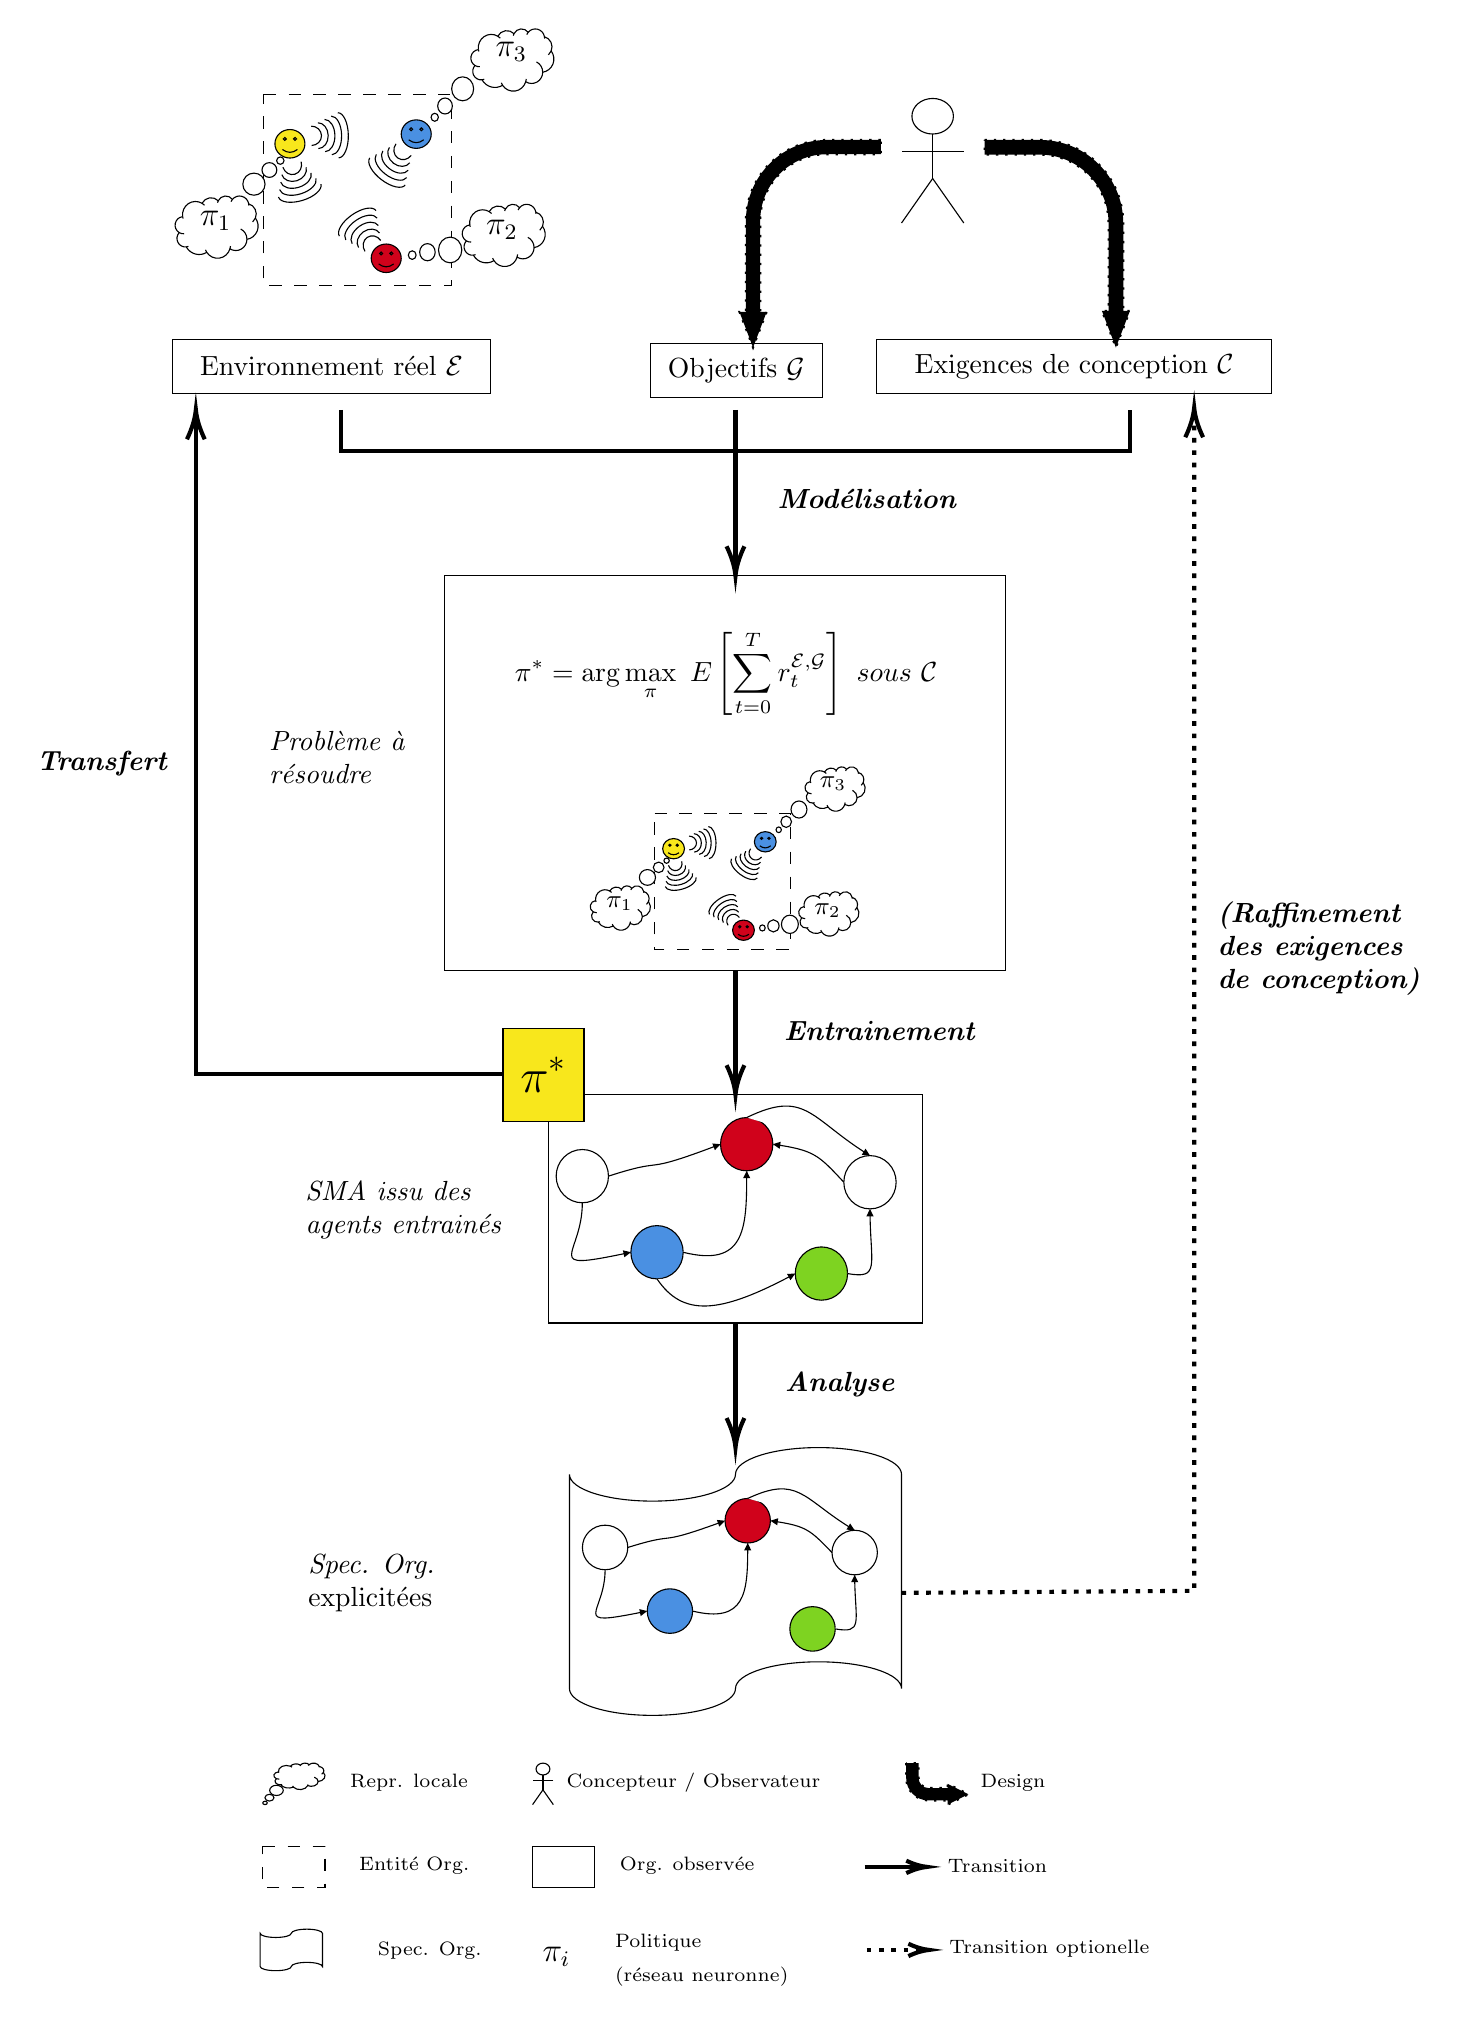
\begin{tikzpicture}[x=0.75pt,y=0.75pt,yscale=-1,xscale=1]
    %uncomment if require: \path (0,3967); %set diagram left start at 0, and has height of 3967

    %Shape: Rectangle [id:dp39157960168103956] 
    \draw  [fill={rgb, 255:red, 255; green, 255; blue, 255 }  ,fill opacity=1 ] (269,3000.97) -- (449,3000.97) -- (449,3110.97) -- (269,3110.97) -- cycle ;
    %Shape: Ellipse [id:dp9935722033847372] 
    \draw  [fill={rgb, 255:red, 255; green, 255; blue, 255 }  ,fill opacity=1 ] (272.6,3040.2) .. controls (272.6,3033.11) and (278.24,3027.37) .. (285.2,3027.37) .. controls (292.16,3027.37) and (297.8,3033.11) .. (297.8,3040.2) .. controls (297.8,3047.29) and (292.16,3053.03) .. (285.2,3053.03) .. controls (278.24,3053.03) and (272.6,3047.29) .. (272.6,3040.2) -- cycle ;
    %Shape: Ellipse [id:dp10593098470820161] 
    \draw  [fill={rgb, 255:red, 74; green, 144; blue, 226 }  ,fill opacity=1 ] (308.6,3076.87) .. controls (308.6,3069.78) and (314.24,3064.03) .. (321.2,3064.03) .. controls (328.16,3064.03) and (333.8,3069.78) .. (333.8,3076.87) .. controls (333.8,3083.96) and (328.16,3089.7) .. (321.2,3089.7) .. controls (314.24,3089.7) and (308.6,3083.96) .. (308.6,3076.87) -- cycle ;
    %Shape: Ellipse [id:dp9599003870836138] 
    \draw  [fill={rgb, 255:red, 208; green, 2; blue, 27 }  ,fill opacity=1 ] (351.8,3024.8) .. controls (351.8,3017.71) and (357.44,3011.97) .. (364.4,3011.97) .. controls (371.36,3011.97) and (377,3017.71) .. (377,3024.8) .. controls (377,3031.89) and (371.36,3037.63) .. (364.4,3037.63) .. controls (357.44,3037.63) and (351.8,3031.89) .. (351.8,3024.8) -- cycle ;
    %Shape: Ellipse [id:dp6518763640259156] 
    \draw  [fill={rgb, 255:red, 255; green, 255; blue, 255 }  ,fill opacity=1 ] (411.2,3043.13) .. controls (411.2,3036.05) and (416.84,3030.3) .. (423.8,3030.3) .. controls (430.76,3030.3) and (436.4,3036.05) .. (436.4,3043.13) .. controls (436.4,3050.22) and (430.76,3055.97) .. (423.8,3055.97) .. controls (416.84,3055.97) and (411.2,3050.22) .. (411.2,3043.13) -- cycle ;
    %Shape: Ellipse [id:dp9715345706408867] 
    \draw  [fill={rgb, 255:red, 126; green, 211; blue, 33 }  ,fill opacity=1 ] (387.8,3087.13) .. controls (387.8,3080.05) and (393.44,3074.3) .. (400.4,3074.3) .. controls (407.36,3074.3) and (413,3080.05) .. (413,3087.13) .. controls (413,3094.22) and (407.36,3099.97) .. (400.4,3099.97) .. controls (393.44,3099.97) and (387.8,3094.22) .. (387.8,3087.13) -- cycle ;
    %Curve Lines [id:da883230177824456] 
    \draw [fill={rgb, 255:red, 255; green, 255; blue, 255 }  ,fill opacity=1 ]   (297.8,3040.2) .. controls (327.79,3030.5) and (311.1,3040.17) .. (349.39,3025.72) ;
    \draw [shift={(351.8,3024.8)}, rotate = 159.15] [fill={rgb, 255:red, 0; green, 0; blue, 0 }  ][line width=0.08]  [draw opacity=0] (3.57,-1.72) -- (0,0) -- (3.57,1.72) -- cycle    ;
    %Curve Lines [id:da5139621017700224] 
    \draw [fill={rgb, 255:red, 255; green, 255; blue, 255 }  ,fill opacity=1 ]   (333.8,3076.87) .. controls (363.33,3084.3) and (364.36,3065.78) .. (364.4,3040.42) ;
    \draw [shift={(364.4,3037.63)}, rotate = 90] [fill={rgb, 255:red, 0; green, 0; blue, 0 }  ][line width=0.08]  [draw opacity=0] (3.57,-1.72) -- (0,0) -- (3.57,1.72) -- cycle    ;
    %Curve Lines [id:da31142570739384423] 
    \draw [fill={rgb, 255:red, 255; green, 255; blue, 255 }  ,fill opacity=1 ]   (411.2,3043.13) .. controls (399.23,3030.25) and (397.01,3027.95) .. (379.84,3025.23) ;
    \draw [shift={(377,3024.8)}, rotate = 8.43] [fill={rgb, 255:red, 0; green, 0; blue, 0 }  ][line width=0.08]  [draw opacity=0] (3.57,-1.72) -- (0,0) -- (3.57,1.72) -- cycle    ;
    %Curve Lines [id:da6742560121764545] 
    \draw [fill={rgb, 255:red, 255; green, 255; blue, 255 }  ,fill opacity=1 ]   (413,3087.13) .. controls (428.63,3089.97) and (424.15,3083.24) .. (423.82,3058.71) ;
    \draw [shift={(423.8,3055.97)}, rotate = 90] [fill={rgb, 255:red, 0; green, 0; blue, 0 }  ][line width=0.08]  [draw opacity=0] (3.57,-1.72) -- (0,0) -- (3.57,1.72) -- cycle    ;
    %Curve Lines [id:da9202599565974993] 
    \draw [fill={rgb, 255:red, 255; green, 255; blue, 255 }  ,fill opacity=1 ]   (285.2,3053.03) .. controls (285.2,3078.55) and (264.46,3086.1) .. (305.98,3077.42) ;
    \draw [shift={(308.6,3076.87)}, rotate = 168.04] [fill={rgb, 255:red, 0; green, 0; blue, 0 }  ][line width=0.08]  [draw opacity=0] (3.57,-1.72) -- (0,0) -- (3.57,1.72) -- cycle    ;
    %Curve Lines [id:da7585089826746155] 
    \draw [fill={rgb, 255:red, 255; green, 255; blue, 255 }  ,fill opacity=1 ]   (321.2,3089.7) .. controls (333.55,3108.03) and (351.08,3106.63) .. (385.66,3088.28) ;
    \draw [shift={(387.8,3087.13)}, rotate = 151.64] [fill={rgb, 255:red, 0; green, 0; blue, 0 }  ][line width=0.08]  [draw opacity=0] (3.57,-1.72) -- (0,0) -- (3.57,1.72) -- cycle    ;
    %Curve Lines [id:da9055022962664225] 
    \draw [fill={rgb, 255:red, 255; green, 255; blue, 255 }  ,fill opacity=1 ]   (364.4,3011.97) .. controls (392.34,2998.45) and (394.87,3011.85) .. (421.28,3028.73) ;
    \draw [shift={(423.8,3030.3)}, rotate = 211.43] [fill={rgb, 255:red, 0; green, 0; blue, 0 }  ][line width=0.08]  [draw opacity=0] (3.57,-1.72) -- (0,0) -- (3.57,1.72) -- cycle    ;
    %Shape: Rectangle [id:dp1660844159337831] 
    \draw  [dash pattern={on 4.5pt off 4.5pt}] (319.98,2865.49) -- (385.59,2865.49) -- (385.59,2930.97) -- (319.98,2930.97) -- cycle ;
    %Shape: Smiley Face [id:dp8672473520454604] 
    \draw  [fill={rgb, 255:red, 248; green, 231; blue, 28 }  ,fill opacity=1 ] (323.92,2882.43) .. controls (323.92,2879.73) and (326.27,2877.54) .. (329.17,2877.54) .. controls (332.07,2877.54) and (334.42,2879.73) .. (334.42,2882.43) .. controls (334.42,2885.13) and (332.07,2887.31) .. (329.17,2887.31) .. controls (326.27,2887.31) and (323.92,2885.13) .. (323.92,2882.43) -- cycle ; \draw  [fill={rgb, 255:red, 248; green, 231; blue, 28 }  ,fill opacity=1 ] (326.86,2880.76) .. controls (326.86,2880.49) and (327.1,2880.27) .. (327.39,2880.27) .. controls (327.68,2880.27) and (327.91,2880.49) .. (327.91,2880.76) .. controls (327.91,2881.03) and (327.68,2881.25) .. (327.39,2881.25) .. controls (327.1,2881.25) and (326.86,2881.03) .. (326.86,2880.76) -- cycle ; \draw  [fill={rgb, 255:red, 248; green, 231; blue, 28 }  ,fill opacity=1 ] (330.43,2880.76) .. controls (330.43,2880.49) and (330.66,2880.27) .. (330.95,2880.27) .. controls (331.24,2880.27) and (331.48,2880.49) .. (331.48,2880.76) .. controls (331.48,2881.03) and (331.24,2881.25) .. (330.95,2881.25) .. controls (330.66,2881.25) and (330.43,2881.03) .. (330.43,2880.76) -- cycle ; \draw   (326.55,2884.38) .. controls (328.3,2885.68) and (330.04,2885.68) .. (331.79,2884.38) ;
    %Shape: Arc [id:dp991830891477531] 
    \draw  [draw opacity=0] (340.03,2896.26) .. controls (340.03,2896.26) and (340.03,2896.26) .. (340.03,2896.26) .. controls (340.58,2898.12) and (337.71,2900.62) .. (333.6,2901.84) .. controls (329.5,2903.07) and (325.72,2902.55) .. (325.17,2900.69) -- (332.6,2898.48) -- cycle ; \draw   (340.03,2896.26) .. controls (340.03,2896.26) and (340.03,2896.26) .. (340.03,2896.26) .. controls (340.58,2898.12) and (337.71,2900.62) .. (333.6,2901.84) .. controls (329.5,2903.07) and (325.72,2902.55) .. (325.17,2900.69) ;
    %Shape: Arc [id:dp15270734978357758] 
    \draw  [draw opacity=0] (338.29,2894.33) .. controls (338.29,2894.33) and (338.29,2894.33) .. (338.29,2894.33) .. controls (338.85,2896.19) and (336.45,2898.55) .. (332.93,2899.6) .. controls (329.41,2900.65) and (326.11,2899.99) .. (325.55,2898.13) -- (331.92,2896.23) -- cycle ; \draw   (338.29,2894.33) .. controls (338.29,2894.33) and (338.29,2894.33) .. (338.29,2894.33) .. controls (338.85,2896.19) and (336.45,2898.55) .. (332.93,2899.6) .. controls (329.41,2900.65) and (326.11,2899.99) .. (325.55,2898.13) ;
    %Shape: Arc [id:dp4538189986822303] 
    \draw  [draw opacity=0] (336.56,2892.4) .. controls (336.56,2892.4) and (336.56,2892.4) .. (336.56,2892.4) .. controls (337.12,2894.26) and (335.19,2896.48) .. (332.26,2897.35) .. controls (329.33,2898.23) and (326.5,2897.43) .. (325.94,2895.57) -- (331.25,2893.99) -- cycle ; \draw   (336.56,2892.4) .. controls (336.56,2892.4) and (336.56,2892.4) .. (336.56,2892.4) .. controls (337.12,2894.26) and (335.19,2896.48) .. (332.26,2897.35) .. controls (329.33,2898.23) and (326.5,2897.43) .. (325.94,2895.57) ;
    %Shape: Arc [id:dp15781801722963062] 
    \draw  [draw opacity=0] (334.83,2890.48) .. controls (334.83,2890.48) and (334.83,2890.48) .. (334.83,2890.48) .. controls (335.38,2892.34) and (333.93,2894.41) .. (331.59,2895.11) .. controls (329.24,2895.81) and (326.89,2894.87) .. (326.33,2893.01) -- (330.58,2891.74) -- cycle ; \draw   (334.83,2890.48) .. controls (334.83,2890.48) and (334.83,2890.48) .. (334.83,2890.48) .. controls (335.38,2892.34) and (333.93,2894.41) .. (331.59,2895.11) .. controls (329.24,2895.81) and (326.89,2894.87) .. (326.33,2893.01) ;
    %Shape: Arc [id:dp647877332552287] 
    \draw  [draw opacity=0] (333.09,2888.55) .. controls (333.09,2888.55) and (333.09,2888.55) .. (333.09,2888.55) .. controls (333.65,2890.41) and (332.67,2892.34) .. (330.92,2892.87) .. controls (329.16,2893.39) and (327.28,2892.31) .. (326.72,2890.45) -- (329.91,2889.5) -- cycle ; \draw   (333.09,2888.55) .. controls (333.09,2888.55) and (333.09,2888.55) .. (333.09,2888.55) .. controls (333.65,2890.41) and (332.67,2892.34) .. (330.92,2892.87) .. controls (329.16,2893.39) and (327.28,2892.31) .. (326.72,2890.45) ;

    %Shape: Arc [id:dp12725807408272582] 
    \draw  [draw opacity=0] (345.93,2871.77) .. controls (345.93,2871.77) and (345.93,2871.77) .. (345.93,2871.77) .. controls (345.93,2871.77) and (345.93,2871.77) .. (345.93,2871.77) .. controls (347.87,2871.73) and (349.51,2875.16) .. (349.6,2879.44) .. controls (349.68,2883.71) and (348.17,2887.21) .. (346.23,2887.25) -- (346.08,2879.51) -- cycle ; \draw   (345.93,2871.77) .. controls (345.93,2871.77) and (345.93,2871.77) .. (345.93,2871.77) .. controls (345.93,2871.77) and (345.93,2871.77) .. (345.93,2871.77) .. controls (347.87,2871.73) and (349.51,2875.16) .. (349.6,2879.44) .. controls (349.68,2883.71) and (348.17,2887.21) .. (346.23,2887.25) ;
    %Shape: Arc [id:dp0663511362149849] 
    \draw  [draw opacity=0] (343.6,2872.92) .. controls (343.6,2872.92) and (343.6,2872.92) .. (343.6,2872.92) .. controls (345.54,2872.88) and (347.18,2875.82) .. (347.25,2879.48) .. controls (347.32,2883.15) and (345.81,2886.15) .. (343.86,2886.19) -- (343.73,2879.55) -- cycle ; \draw   (343.6,2872.92) .. controls (343.6,2872.92) and (343.6,2872.92) .. (343.6,2872.92) .. controls (345.54,2872.88) and (347.18,2875.82) .. (347.25,2879.48) .. controls (347.32,2883.15) and (345.81,2886.15) .. (343.86,2886.19) ;
    %Shape: Arc [id:dp5596459802099086] 
    \draw  [draw opacity=0] (341.28,2874.07) .. controls (341.28,2874.07) and (341.28,2874.07) .. (341.28,2874.07) .. controls (343.22,2874.03) and (344.84,2876.48) .. (344.9,2879.53) .. controls (344.97,2882.58) and (343.44,2885.09) .. (341.49,2885.13) -- (341.38,2879.6) -- cycle ; \draw   (341.28,2874.07) .. controls (341.28,2874.07) and (341.28,2874.07) .. (341.28,2874.07) .. controls (343.22,2874.03) and (344.84,2876.48) .. (344.9,2879.53) .. controls (344.97,2882.58) and (343.44,2885.09) .. (341.49,2885.13) ;
    %Shape: Arc [id:dp939679467729508] 
    \draw  [draw opacity=0] (338.95,2875.22) .. controls (338.95,2875.22) and (338.95,2875.22) .. (338.95,2875.22) .. controls (340.9,2875.18) and (342.51,2877.13) .. (342.56,2879.58) .. controls (342.61,2882.02) and (341.07,2884.03) .. (339.13,2884.07) -- (339.04,2879.65) -- cycle ; \draw   (338.95,2875.22) .. controls (338.95,2875.22) and (338.95,2875.22) .. (338.95,2875.22) .. controls (340.9,2875.18) and (342.51,2877.13) .. (342.56,2879.58) .. controls (342.61,2882.02) and (341.07,2884.03) .. (339.13,2884.07) ;
    %Shape: Arc [id:dp4187174998399785] 
    \draw  [draw opacity=0] (336.63,2876.37) .. controls (336.63,2876.37) and (336.63,2876.37) .. (336.63,2876.37) .. controls (338.57,2876.34) and (340.18,2877.79) .. (340.21,2879.62) .. controls (340.25,2881.45) and (338.7,2882.97) .. (336.76,2883.01) -- (336.69,2879.69) -- cycle ; \draw   (336.63,2876.37) .. controls (336.63,2876.37) and (336.63,2876.37) .. (336.63,2876.37) .. controls (338.57,2876.34) and (340.18,2877.79) .. (340.21,2879.62) .. controls (340.25,2881.45) and (338.7,2882.97) .. (336.76,2883.01) ;

    %Shape: Smiley Face [id:dp2664344043944723] 
    \draw  [fill={rgb, 255:red, 208; green, 2; blue, 27 }  ,fill opacity=1 ] (357.6,2921.71) .. controls (357.6,2919.01) and (359.95,2916.82) .. (362.85,2916.82) .. controls (365.75,2916.82) and (368.1,2919.01) .. (368.1,2921.71) .. controls (368.1,2924.41) and (365.75,2926.6) .. (362.85,2926.6) .. controls (359.95,2926.6) and (357.6,2924.41) .. (357.6,2921.71) -- cycle ; \draw  [fill={rgb, 255:red, 208; green, 2; blue, 27 }  ,fill opacity=1 ] (360.54,2920.05) .. controls (360.54,2919.78) and (360.78,2919.56) .. (361.07,2919.56) .. controls (361.36,2919.56) and (361.59,2919.78) .. (361.59,2920.05) .. controls (361.59,2920.32) and (361.36,2920.54) .. (361.07,2920.54) .. controls (360.78,2920.54) and (360.54,2920.32) .. (360.54,2920.05) -- cycle ; \draw  [fill={rgb, 255:red, 208; green, 2; blue, 27 }  ,fill opacity=1 ] (364.11,2920.05) .. controls (364.11,2919.78) and (364.34,2919.56) .. (364.63,2919.56) .. controls (364.92,2919.56) and (365.16,2919.78) .. (365.16,2920.05) .. controls (365.16,2920.32) and (364.92,2920.54) .. (364.63,2920.54) .. controls (364.34,2920.54) and (364.11,2920.32) .. (364.11,2920.05) -- cycle ; \draw   (360.23,2923.67) .. controls (361.98,2924.97) and (363.72,2924.97) .. (365.47,2923.67) ;
    %Shape: Arc [id:dp7671134474873877] 
    \draw  [draw opacity=0] (346.47,2914.11) .. controls (346.47,2914.11) and (346.47,2914.11) .. (346.47,2914.11) .. controls (345.37,2912.51) and (347.34,2909.26) .. (350.88,2906.84) .. controls (354.41,2904.42) and (358.16,2903.76) .. (359.26,2905.36) -- (352.87,2909.74) -- cycle ; \draw   (346.47,2914.11) .. controls (346.47,2914.11) and (346.47,2914.11) .. (346.47,2914.11) .. controls (345.37,2912.51) and (347.34,2909.26) .. (350.88,2906.84) .. controls (354.41,2904.42) and (358.16,2903.76) .. (359.26,2905.36) ;
    %Shape: Arc [id:dp7465446437475772] 
    \draw  [draw opacity=0] (348.71,2915.42) .. controls (348.71,2915.42) and (348.71,2915.42) .. (348.71,2915.42) .. controls (347.61,2913.82) and (349.18,2910.84) .. (352.2,2908.77) .. controls (355.23,2906.7) and (358.58,2906.32) .. (359.68,2907.92) .. controls (359.68,2907.92) and (359.68,2907.92) .. (359.68,2907.92) -- (354.19,2911.67) -- cycle ; \draw   (348.71,2915.42) .. controls (348.71,2915.42) and (348.71,2915.42) .. (348.71,2915.42) .. controls (347.61,2913.82) and (349.18,2910.84) .. (352.2,2908.77) .. controls (355.23,2906.7) and (358.58,2906.32) .. (359.68,2907.92) .. controls (359.68,2907.92) and (359.68,2907.92) .. (359.68,2907.92) ;
    %Shape: Arc [id:dp9770041114548759] 
    \draw  [draw opacity=0] (350.95,2916.73) .. controls (350.95,2916.73) and (350.95,2916.73) .. (350.95,2916.73) .. controls (350.95,2916.73) and (350.95,2916.73) .. (350.95,2916.73) .. controls (349.85,2915.13) and (351.01,2912.43) .. (353.53,2910.7) .. controls (356.05,2908.98) and (358.99,2908.87) .. (360.09,2910.47) -- (355.52,2913.6) -- cycle ; \draw   (350.95,2916.73) .. controls (350.95,2916.73) and (350.95,2916.73) .. (350.95,2916.73) .. controls (350.95,2916.73) and (350.95,2916.73) .. (350.95,2916.73) .. controls (349.85,2915.13) and (351.01,2912.43) .. (353.53,2910.7) .. controls (356.05,2908.98) and (358.99,2908.87) .. (360.09,2910.47) ;
    %Shape: Arc [id:dp4418659452921887] 
    \draw  [draw opacity=0] (353.19,2918.03) .. controls (353.19,2918.03) and (353.19,2918.03) .. (353.19,2918.03) .. controls (353.19,2918.03) and (353.19,2918.03) .. (353.19,2918.03) .. controls (352.09,2916.43) and (352.84,2914.02) .. (354.86,2912.63) .. controls (356.88,2911.25) and (359.4,2911.43) .. (360.5,2913.03) -- (356.85,2915.53) -- cycle ; \draw   (353.19,2918.03) .. controls (353.19,2918.03) and (353.19,2918.03) .. (353.19,2918.03) .. controls (353.19,2918.03) and (353.19,2918.03) .. (353.19,2918.03) .. controls (352.09,2916.43) and (352.84,2914.02) .. (354.86,2912.63) .. controls (356.88,2911.25) and (359.4,2911.43) .. (360.5,2913.03) ;
    %Shape: Arc [id:dp6696566494284376] 
    \draw  [draw opacity=0] (355.43,2919.34) .. controls (355.43,2919.34) and (355.43,2919.34) .. (355.43,2919.34) .. controls (354.34,2917.74) and (354.67,2915.6) .. (356.18,2914.57) .. controls (357.7,2913.53) and (359.82,2913.99) .. (360.92,2915.59) -- (358.18,2917.46) -- cycle ; \draw   (355.43,2919.34) .. controls (355.43,2919.34) and (355.43,2919.34) .. (355.43,2919.34) .. controls (354.34,2917.74) and (354.67,2915.6) .. (356.18,2914.57) .. controls (357.7,2913.53) and (359.82,2913.99) .. (360.92,2915.59) ;

    %Shape: Smiley Face [id:dp09777682624392658] 
    \draw  [fill={rgb, 255:red, 74; green, 144; blue, 226 }  ,fill opacity=1 ] (368.1,2879.11) .. controls (368.1,2876.41) and (370.45,2874.22) .. (373.35,2874.22) .. controls (376.25,2874.22) and (378.6,2876.41) .. (378.6,2879.11) .. controls (378.6,2881.81) and (376.25,2884) .. (373.35,2884) .. controls (370.45,2884) and (368.1,2881.81) .. (368.1,2879.11) -- cycle ; \draw  [fill={rgb, 255:red, 74; green, 144; blue, 226 }  ,fill opacity=1 ] (371.04,2877.45) .. controls (371.04,2877.18) and (371.27,2876.96) .. (371.56,2876.96) .. controls (371.85,2876.96) and (372.09,2877.18) .. (372.09,2877.45) .. controls (372.09,2877.72) and (371.85,2877.93) .. (371.56,2877.93) .. controls (371.27,2877.93) and (371.04,2877.72) .. (371.04,2877.45) -- cycle ; \draw  [fill={rgb, 255:red, 74; green, 144; blue, 226 }  ,fill opacity=1 ] (374.61,2877.45) .. controls (374.61,2877.18) and (374.84,2876.96) .. (375.13,2876.96) .. controls (375.42,2876.96) and (375.66,2877.18) .. (375.66,2877.45) .. controls (375.66,2877.72) and (375.42,2877.93) .. (375.13,2877.93) .. controls (374.84,2877.93) and (374.61,2877.72) .. (374.61,2877.45) -- cycle ; \draw   (370.72,2881.06) .. controls (372.47,2882.37) and (374.22,2882.37) .. (375.97,2881.06) ;
    %Shape: Arc [id:dp7162316795920435] 
    \draw  [draw opacity=0] (369.5,2896.57) .. controls (368.33,2898.12) and (364.61,2897.3) .. (361.18,2894.74) .. controls (357.76,2892.18) and (355.92,2888.84) .. (357.09,2887.29) .. controls (357.09,2887.29) and (357.09,2887.29) .. (357.09,2887.29) -- (363.29,2891.93) -- cycle ; \draw   (369.5,2896.57) .. controls (368.33,2898.12) and (364.61,2897.3) .. (361.18,2894.74) .. controls (357.76,2892.18) and (355.92,2888.84) .. (357.09,2887.29) .. controls (357.09,2887.29) and (357.09,2887.29) .. (357.09,2887.29) ;
    %Shape: Arc [id:dp412134008181967] 
    \draw  [draw opacity=0] (370.02,2894.03) .. controls (370.02,2894.03) and (370.02,2894.03) .. (370.02,2894.03) .. controls (370.02,2894.03) and (370.02,2894.03) .. (370.02,2894.03) .. controls (368.86,2895.59) and (365.53,2895.06) .. (362.59,2892.87) .. controls (359.65,2890.67) and (358.22,2887.63) .. (359.38,2886.08) .. controls (359.38,2886.08) and (359.38,2886.08) .. (359.38,2886.08) -- (364.7,2890.06) -- cycle ; \draw   (370.02,2894.03) .. controls (370.02,2894.03) and (370.02,2894.03) .. (370.02,2894.03) .. controls (370.02,2894.03) and (370.02,2894.03) .. (370.02,2894.03) .. controls (368.86,2895.59) and (365.53,2895.06) .. (362.59,2892.87) .. controls (359.65,2890.67) and (358.22,2887.63) .. (359.38,2886.08) .. controls (359.38,2886.08) and (359.38,2886.08) .. (359.38,2886.08) ;
    %Shape: Arc [id:dp9457493036891829] 
    \draw  [draw opacity=0] (370.54,2891.5) .. controls (370.54,2891.5) and (370.54,2891.5) .. (370.54,2891.5) .. controls (370.54,2891.5) and (370.54,2891.5) .. (370.54,2891.5) .. controls (369.38,2893.05) and (366.45,2892.82) .. (364,2890.99) .. controls (361.55,2889.16) and (360.51,2886.42) .. (361.68,2884.87) -- (366.11,2888.18) -- cycle ; \draw   (370.54,2891.5) .. controls (370.54,2891.5) and (370.54,2891.5) .. (370.54,2891.5) .. controls (370.54,2891.5) and (370.54,2891.5) .. (370.54,2891.5) .. controls (369.38,2893.05) and (366.45,2892.82) .. (364,2890.99) .. controls (361.55,2889.16) and (360.51,2886.42) .. (361.68,2884.87) ;
    %Shape: Arc [id:dp6838488823519279] 
    \draw  [draw opacity=0] (371.06,2888.96) .. controls (371.06,2888.96) and (371.06,2888.96) .. (371.06,2888.96) .. controls (369.9,2890.51) and (367.36,2890.58) .. (365.41,2889.12) .. controls (363.45,2887.65) and (362.8,2885.21) .. (363.97,2883.65) -- (367.52,2886.31) -- cycle ; \draw   (371.06,2888.96) .. controls (371.06,2888.96) and (371.06,2888.96) .. (371.06,2888.96) .. controls (369.9,2890.51) and (367.36,2890.58) .. (365.41,2889.12) .. controls (363.45,2887.65) and (362.8,2885.21) .. (363.97,2883.65) ;
    %Shape: Arc [id:dp5242677755784311] 
    \draw  [draw opacity=0] (371.58,2886.42) .. controls (371.58,2886.42) and (371.58,2886.42) .. (371.58,2886.42) .. controls (371.58,2886.42) and (371.58,2886.42) .. (371.58,2886.42) .. controls (370.42,2887.97) and (368.28,2888.34) .. (366.81,2887.24) .. controls (365.34,2886.15) and (365.1,2884) .. (366.26,2882.44) -- (368.92,2884.43) -- cycle ; \draw   (371.58,2886.42) .. controls (371.58,2886.42) and (371.58,2886.42) .. (371.58,2886.42) .. controls (371.58,2886.42) and (371.58,2886.42) .. (371.58,2886.42) .. controls (370.42,2887.97) and (368.28,2888.34) .. (366.81,2887.24) .. controls (365.34,2886.15) and (365.1,2884) .. (366.26,2882.44) ;

    %Shape: Cloud [id:dp4236644517840452] 
    \draw  [fill={rgb, 255:red, 255; green, 255; blue, 255 }  ,fill opacity=1 ] (291.64,2907.38) .. controls (291.41,2905.65) and (292.18,2903.95) .. (293.62,2902.98) .. controls (295.06,2902.02) and (296.93,2901.96) .. (298.43,2902.84) .. controls (298.96,2901.84) and (299.93,2901.15) .. (301.05,2900.98) .. controls (302.16,2900.81) and (303.29,2901.17) .. (304.1,2901.97) .. controls (304.55,2901.06) and (305.44,2900.45) .. (306.45,2900.35) .. controls (307.45,2900.26) and (308.44,2900.69) .. (309.05,2901.5) .. controls (309.87,2900.54) and (311.17,2900.13) .. (312.39,2900.46) .. controls (313.61,2900.79) and (314.53,2901.79) .. (314.75,2903.03) .. controls (315.75,2903.3) and (316.58,2904) .. (317.03,2904.93) .. controls (317.48,2905.87) and (317.51,2906.96) .. (317.1,2907.92) .. controls (318.08,2909.2) and (318.31,2910.91) .. (317.7,2912.41) .. controls (317.1,2913.91) and (315.74,2914.98) .. (314.14,2915.2) .. controls (314.12,2916.61) and (313.35,2917.9) .. (312.12,2918.58) .. controls (310.89,2919.26) and (309.39,2919.22) .. (308.2,2918.47) .. controls (307.69,2920.16) and (306.26,2921.4) .. (304.52,2921.66) .. controls (302.79,2921.92) and (301.06,2921.15) .. (300.09,2919.68) .. controls (298.89,2920.41) and (297.46,2920.61) .. (296.11,2920.26) .. controls (294.76,2919.91) and (293.61,2919.02) .. (292.92,2917.81) .. controls (291.7,2917.95) and (290.52,2917.32) .. (289.97,2916.22) .. controls (289.41,2915.13) and (289.6,2913.8) .. (290.44,2912.9) .. controls (289.35,2912.26) and (288.8,2910.99) .. (289.07,2909.74) .. controls (289.33,2908.5) and (290.36,2907.57) .. (291.62,2907.44) ; \draw   (290.44,2912.9) .. controls (290.96,2913.21) and (291.55,2913.34) .. (292.14,2913.3)(292.92,2917.81) .. controls (293.18,2917.78) and (293.43,2917.72) .. (293.67,2917.62)(300.09,2919.68) .. controls (299.91,2919.41) and (299.76,2919.13) .. (299.64,2918.82)(308.2,2918.47) .. controls (308.29,2918.17) and (308.35,2917.85) .. (308.38,2917.53)(314.14,2915.2) .. controls (314.15,2913.71) and (313.3,2912.33) .. (311.95,2911.68)(317.1,2907.92) .. controls (316.88,2908.43) and (316.55,2908.88) .. (316.13,2909.24)(314.75,2903.03) .. controls (314.79,2903.23) and (314.8,2903.44) .. (314.8,2903.65)(309.05,2901.5) .. controls (308.85,2901.74) and (308.68,2902.01) .. (308.56,2902.3)(304.1,2901.97) .. controls (303.99,2902.19) and (303.91,2902.42) .. (303.86,2902.66)(298.43,2902.84) .. controls (298.74,2903.03) and (299.04,2903.25) .. (299.3,2903.51)(291.64,2907.38) .. controls (291.67,2907.61) and (291.73,2907.85) .. (291.79,2908.08) ;
    %Shape: Cloud [id:dp9261610463414396] 
    \draw  [fill={rgb, 255:red, 255; green, 255; blue, 255 }  ,fill opacity=1 ] (395.1,2850.04) .. controls (394.87,2848.32) and (395.64,2846.61) .. (397.08,2845.65) .. controls (398.52,2844.68) and (400.39,2844.63) .. (401.89,2845.51) .. controls (402.42,2844.51) and (403.39,2843.82) .. (404.5,2843.64) .. controls (405.62,2843.47) and (406.75,2843.84) .. (407.56,2844.63) .. controls (408.01,2843.73) and (408.9,2843.12) .. (409.91,2843.02) .. controls (410.91,2842.92) and (411.9,2843.36) .. (412.51,2844.16) .. controls (413.33,2843.2) and (414.63,2842.8) .. (415.85,2843.12) .. controls (417.06,2843.45) and (417.98,2844.45) .. (418.21,2845.69) .. controls (419.21,2845.97) and (420.04,2846.66) .. (420.49,2847.6) .. controls (420.94,2848.54) and (420.97,2849.62) .. (420.56,2850.58) .. controls (421.54,2851.87) and (421.77,2853.58) .. (421.16,2855.08) .. controls (420.55,2856.58) and (419.2,2857.64) .. (417.6,2857.87) .. controls (417.58,2859.28) and (416.81,2860.57) .. (415.58,2861.25) .. controls (414.35,2861.93) and (412.85,2861.88) .. (411.65,2861.14) .. controls (411.15,2862.82) and (409.72,2864.06) .. (407.98,2864.32) .. controls (406.25,2864.58) and (404.52,2863.81) .. (403.55,2862.35) .. controls (402.35,2863.07) and (400.92,2863.28) .. (399.57,2862.93) .. controls (398.22,2862.57) and (397.07,2861.69) .. (396.38,2860.47) .. controls (395.16,2860.62) and (393.98,2859.98) .. (393.43,2858.89) .. controls (392.87,2857.79) and (393.06,2856.46) .. (393.9,2855.57) .. controls (392.81,2854.93) and (392.26,2853.65) .. (392.53,2852.41) .. controls (392.79,2851.17) and (393.82,2850.24) .. (395.08,2850.11) ; \draw   (393.9,2855.57) .. controls (394.42,2855.87) and (395.01,2856.01) .. (395.6,2855.96)(396.38,2860.47) .. controls (396.64,2860.44) and (396.89,2860.38) .. (397.12,2860.28)(403.55,2862.35) .. controls (403.37,2862.08) and (403.22,2861.79) .. (403.1,2861.49)(411.65,2861.14) .. controls (411.75,2860.83) and (411.81,2860.51) .. (411.83,2860.19)(417.59,2857.87) .. controls (417.61,2856.37) and (416.76,2855) .. (415.41,2854.34)(420.56,2850.58) .. controls (420.34,2851.09) and (420.01,2851.54) .. (419.59,2851.9)(418.21,2845.69) .. controls (418.25,2845.9) and (418.26,2846.11) .. (418.26,2846.32)(412.51,2844.16) .. controls (412.31,2844.4) and (412.14,2844.67) .. (412.01,2844.96)(407.56,2844.63) .. controls (407.45,2844.85) and (407.37,2845.08) .. (407.32,2845.32)(401.89,2845.51) .. controls (402.2,2845.69) and (402.5,2845.92) .. (402.76,2846.18)(395.1,2850.04) .. controls (395.13,2850.28) and (395.18,2850.51) .. (395.25,2850.74) ;
    %Shape: Ellipse [id:dp38327597242410594] 
    \draw  [fill={rgb, 255:red, 255; green, 255; blue, 255 }  ,fill opacity=1 ] (380.86,2869.46) .. controls (380.86,2867.95) and (382.01,2866.72) .. (383.43,2866.72) .. controls (384.84,2866.72) and (385.99,2867.95) .. (385.99,2869.46) .. controls (385.99,2870.97) and (384.84,2872.2) .. (383.43,2872.2) .. controls (382.01,2872.2) and (380.86,2870.97) .. (380.86,2869.46) -- cycle ;
    %Shape: Ellipse [id:dp0569021122146276] 
    \draw  [fill={rgb, 255:red, 255; green, 255; blue, 255 }  ,fill opacity=1 ] (378.54,2873.33) .. controls (378.54,2872.57) and (379.12,2871.96) .. (379.82,2871.96) .. controls (380.53,2871.96) and (381.11,2872.57) .. (381.11,2873.33) .. controls (381.11,2874.09) and (380.53,2874.7) .. (379.82,2874.7) .. controls (379.12,2874.7) and (378.54,2874.09) .. (378.54,2873.33) -- cycle ;
    %Shape: Ellipse [id:dp908037679999253] 
    \draw  [fill={rgb, 255:red, 255; green, 255; blue, 255 }  ,fill opacity=1 ] (319.4,2891.43) .. controls (319.4,2890.03) and (320.56,2888.9) .. (321.99,2888.9) .. controls (323.42,2888.9) and (324.58,2890.03) .. (324.58,2891.43) .. controls (324.58,2892.82) and (323.42,2893.95) .. (321.99,2893.95) .. controls (320.56,2893.95) and (319.4,2892.82) .. (319.4,2891.43) -- cycle ;
    %Shape: Ellipse [id:dp7926420178535974] 
    \draw  [fill={rgb, 255:red, 255; green, 255; blue, 255 }  ,fill opacity=1 ] (312.69,2896.28) .. controls (312.69,2894.19) and (314.43,2892.49) .. (316.58,2892.49) .. controls (318.72,2892.49) and (320.46,2894.19) .. (320.46,2896.28) .. controls (320.46,2898.38) and (318.72,2900.07) .. (316.58,2900.07) .. controls (314.43,2900.07) and (312.69,2898.38) .. (312.69,2896.28) -- cycle ;
    %Shape: Ellipse [id:dp884513706406913] 
    \draw  [fill={rgb, 255:red, 255; green, 255; blue, 255 }  ,fill opacity=1 ] (324.52,2888.2) .. controls (324.52,2887.51) and (325.1,2886.94) .. (325.81,2886.94) .. controls (326.53,2886.94) and (327.11,2887.51) .. (327.11,2888.2) .. controls (327.11,2888.9) and (326.53,2889.47) .. (325.81,2889.47) .. controls (325.1,2889.47) and (324.52,2888.9) .. (324.52,2888.2) -- cycle ;
    %Shape: Ellipse [id:dp045097605817289055] 
    \draw  [fill={rgb, 255:red, 255; green, 255; blue, 255 }  ,fill opacity=1 ] (385.75,2863.56) .. controls (385.75,2861.29) and (387.47,2859.45) .. (389.59,2859.45) .. controls (391.71,2859.45) and (393.43,2861.29) .. (393.43,2863.56) .. controls (393.43,2865.83) and (391.71,2867.67) .. (389.59,2867.67) .. controls (387.47,2867.67) and (385.75,2865.83) .. (385.75,2863.56) -- cycle ;
    %Shape: Ellipse [id:dp34409865082548896] 
    \draw  [fill={rgb, 255:red, 255; green, 255; blue, 255 }  ,fill opacity=1 ] (381.14,2918.86) .. controls (381.14,2916.42) and (382.97,2914.45) .. (385.22,2914.45) .. controls (387.47,2914.45) and (389.29,2916.42) .. (389.29,2918.86) .. controls (389.29,2921.29) and (387.47,2923.27) .. (385.22,2923.27) .. controls (382.97,2923.27) and (381.14,2921.29) .. (381.14,2918.86) -- cycle ;
    %Shape: Ellipse [id:dp7946586129033605] 
    \draw  [fill={rgb, 255:red, 255; green, 255; blue, 255 }  ,fill opacity=1 ] (374.56,2919.62) .. controls (374.56,2918) and (375.77,2916.68) .. (377.27,2916.68) .. controls (378.77,2916.68) and (379.99,2918) .. (379.99,2919.62) .. controls (379.99,2921.25) and (378.77,2922.56) .. (377.27,2922.56) .. controls (375.77,2922.56) and (374.56,2921.25) .. (374.56,2919.62) -- cycle ;
    %Shape: Ellipse [id:dp8588991503220264] 
    \draw  [fill={rgb, 255:red, 255; green, 255; blue, 255 }  ,fill opacity=1 ] (370.59,2920.62) .. controls (370.59,2919.81) and (371.2,2919.15) .. (371.95,2919.15) .. controls (372.7,2919.15) and (373.31,2919.81) .. (373.31,2920.62) .. controls (373.31,2921.43) and (372.7,2922.09) .. (371.95,2922.09) .. controls (371.2,2922.09) and (370.59,2921.43) .. (370.59,2920.62) -- cycle ;
    %Shape: Cloud [id:dp5704725396428417] 
    \draw  [fill={rgb, 255:red, 255; green, 255; blue, 255 }  ,fill opacity=1 ] (392.08,2910.23) .. controls (391.84,2908.5) and (392.61,2906.8) .. (394.06,2905.83) .. controls (395.5,2904.87) and (397.37,2904.81) .. (398.86,2905.69) .. controls (399.39,2904.69) and (400.36,2904) .. (401.48,2903.83) .. controls (402.6,2903.65) and (403.73,2904.02) .. (404.54,2904.82) .. controls (404.99,2903.91) and (405.87,2903.3) .. (406.88,2903.2) .. controls (407.89,2903.11) and (408.88,2903.54) .. (409.49,2904.35) .. controls (410.31,2903.39) and (411.6,2902.98) .. (412.82,2903.31) .. controls (414.04,2903.63) and (414.96,2904.64) .. (415.19,2905.88) .. controls (416.19,2906.15) and (417.02,2906.85) .. (417.47,2907.78) .. controls (417.92,2908.72) and (417.94,2909.81) .. (417.54,2910.76) .. controls (418.52,2912.05) and (418.75,2913.76) .. (418.14,2915.26) .. controls (417.53,2916.76) and (416.17,2917.82) .. (414.57,2918.05) .. controls (414.56,2919.46) and (413.79,2920.75) .. (412.56,2921.43) .. controls (411.33,2922.11) and (409.82,2922.07) .. (408.63,2921.32) .. controls (408.12,2923.01) and (406.69,2924.25) .. (404.96,2924.51) .. controls (403.23,2924.77) and (401.5,2924) .. (400.52,2922.53) .. controls (399.33,2923.26) and (397.9,2923.46) .. (396.55,2923.11) .. controls (395.2,2922.76) and (394.05,2921.87) .. (393.36,2920.66) .. controls (392.14,2920.8) and (390.96,2920.17) .. (390.4,2919.07) .. controls (389.85,2917.97) and (390.04,2916.65) .. (390.88,2915.75) .. controls (389.79,2915.11) and (389.23,2913.84) .. (389.5,2912.59) .. controls (389.77,2911.35) and (390.8,2910.42) .. (392.05,2910.29) ; \draw   (390.88,2915.75) .. controls (391.39,2916.06) and (391.99,2916.19) .. (392.58,2916.15)(393.36,2920.66) .. controls (393.61,2920.63) and (393.86,2920.56) .. (394.1,2920.47)(400.52,2922.53) .. controls (400.34,2922.26) and (400.19,2921.97) .. (400.08,2921.67)(408.63,2921.32) .. controls (408.72,2921.01) and (408.78,2920.7) .. (408.81,2920.38)(414.57,2918.05) .. controls (414.58,2916.55) and (413.73,2915.18) .. (412.39,2914.53)(417.54,2910.76) .. controls (417.32,2911.27) and (416.98,2911.73) .. (416.56,2912.09)(415.19,2905.88) .. controls (415.22,2906.08) and (415.24,2906.29) .. (415.24,2906.5)(409.49,2904.35) .. controls (409.29,2904.59) and (409.12,2904.86) .. (408.99,2905.14)(404.54,2904.82) .. controls (404.43,2905.04) and (404.35,2905.27) .. (404.3,2905.51)(398.86,2905.69) .. controls (399.18,2905.88) and (399.47,2906.1) .. (399.74,2906.36)(392.08,2910.23) .. controls (392.11,2910.46) and (392.16,2910.7) .. (392.23,2910.93) ;
    %Shape: Rectangle [id:dp2824507959380417] 
    \draw   (219,2750.97) -- (489,2750.97) -- (489,2940.97) -- (219,2940.97) -- cycle ;
    %Flowchart: Punched Tape [id:dp9081855054145813] 
    \draw  [fill={rgb, 255:red, 255; green, 255; blue, 255 }  ,fill opacity=1 ] (279,3183.87) .. controls (279,3191) and (296.91,3196.77) .. (319,3196.77) .. controls (341.09,3196.77) and (359,3191) .. (359,3183.87) .. controls (359,3176.74) and (376.91,3170.97) .. (399,3170.97) .. controls (421.09,3170.97) and (439,3176.74) .. (439,3183.87) -- (439,3287.1) .. controls (439,3279.97) and (421.09,3274.19) .. (399,3274.19) .. controls (376.91,3274.19) and (359,3279.97) .. (359,3287.1) .. controls (359,3294.22) and (341.09,3300) .. (319,3300) .. controls (296.91,3300) and (279,3294.22) .. (279,3287.1) -- cycle ;
    %Shape: Ellipse [id:dp16129214012888815] 
    \draw  [fill={rgb, 255:red, 255; green, 255; blue, 255 }  ,fill opacity=1 ] (285.25,3219.1) .. controls (285.25,3213.17) and (290.14,3208.37) .. (296.18,3208.37) .. controls (302.22,3208.37) and (307.11,3213.17) .. (307.11,3219.1) .. controls (307.11,3225.02) and (302.22,3229.83) .. (296.18,3229.83) .. controls (290.14,3229.83) and (285.25,3225.02) .. (285.25,3219.1) -- cycle ;
    %Shape: Ellipse [id:dp46629806906917204] 
    \draw  [fill={rgb, 255:red, 74; green, 144; blue, 226 }  ,fill opacity=1 ] (316.48,3249.75) .. controls (316.48,3243.83) and (321.37,3239.02) .. (327.41,3239.02) .. controls (333.45,3239.02) and (338.34,3243.83) .. (338.34,3249.75) .. controls (338.34,3255.68) and (333.45,3260.48) .. (327.41,3260.48) .. controls (321.37,3260.48) and (316.48,3255.68) .. (316.48,3249.75) -- cycle ;
    %Shape: Ellipse [id:dp8639592543358846] 
    \draw  [fill={rgb, 255:red, 208; green, 2; blue, 27 }  ,fill opacity=1 ] (353.96,3206.22) .. controls (353.96,3200.3) and (358.85,3195.49) .. (364.89,3195.49) .. controls (370.93,3195.49) and (375.82,3200.3) .. (375.82,3206.22) .. controls (375.82,3212.15) and (370.93,3216.95) .. (364.89,3216.95) .. controls (358.85,3216.95) and (353.96,3212.15) .. (353.96,3206.22) -- cycle ;
    %Shape: Ellipse [id:dp0625434790011643] 
    \draw  [fill={rgb, 255:red, 255; green, 255; blue, 255 }  ,fill opacity=1 ] (405.5,3221.55) .. controls (405.5,3215.62) and (410.39,3210.82) .. (416.43,3210.82) .. controls (422.46,3210.82) and (427.36,3215.62) .. (427.36,3221.55) .. controls (427.36,3227.48) and (422.46,3232.28) .. (416.43,3232.28) .. controls (410.39,3232.28) and (405.5,3227.48) .. (405.5,3221.55) -- cycle ;
    %Shape: Ellipse [id:dp16572009365052887] 
    \draw  [fill={rgb, 255:red, 126; green, 211; blue, 33 }  ,fill opacity=1 ] (385.19,3258.34) .. controls (385.19,3252.41) and (390.09,3247.61) .. (396.13,3247.61) .. controls (402.16,3247.61) and (407.06,3252.41) .. (407.06,3258.34) .. controls (407.06,3264.26) and (402.16,3269.07) .. (396.13,3269.07) .. controls (390.09,3269.07) and (385.19,3264.26) .. (385.19,3258.34) -- cycle ;
    %Curve Lines [id:da5129135517057147] 
    \draw [fill={rgb, 255:red, 255; green, 255; blue, 255 }  ,fill opacity=1 ]   (307.11,3219.1) .. controls (332.99,3211.03) and (318.8,3218.98) .. (351.36,3207.17) ;
    \draw [shift={(353.96,3206.22)}, rotate = 159.85] [fill={rgb, 255:red, 0; green, 0; blue, 0 }  ][line width=0.08]  [draw opacity=0] (3.57,-1.72) -- (0,0) -- (3.57,1.72) -- cycle    ;
    %Curve Lines [id:da23727674298529522] 
    \draw [fill={rgb, 255:red, 255; green, 255; blue, 255 }  ,fill opacity=1 ]   (338.34,3249.75) .. controls (363.7,3255.9) and (364.84,3240.8) .. (364.89,3219.94) ;
    \draw [shift={(364.89,3216.95)}, rotate = 90] [fill={rgb, 255:red, 0; green, 0; blue, 0 }  ][line width=0.08]  [draw opacity=0] (3.57,-1.72) -- (0,0) -- (3.57,1.72) -- cycle    ;
    %Curve Lines [id:da9799487912929773] 
    \draw [fill={rgb, 255:red, 255; green, 255; blue, 255 }  ,fill opacity=1 ]   (405.5,3221.55) .. controls (395.22,3210.89) and (393.22,3208.89) .. (378.75,3206.66) ;
    \draw [shift={(375.82,3206.22)}, rotate = 8.12] [fill={rgb, 255:red, 0; green, 0; blue, 0 }  ][line width=0.08]  [draw opacity=0] (3.57,-1.72) -- (0,0) -- (3.57,1.72) -- cycle    ;
    %Curve Lines [id:da5937531433947929] 
    \draw [fill={rgb, 255:red, 255; green, 255; blue, 255 }  ,fill opacity=1 ]   (407.06,3258.34) .. controls (420.48,3260.68) and (416.81,3255.19) .. (416.45,3235.2) ;
    \draw [shift={(416.43,3232.28)}, rotate = 90] [fill={rgb, 255:red, 0; green, 0; blue, 0 }  ][line width=0.08]  [draw opacity=0] (3.57,-1.72) -- (0,0) -- (3.57,1.72) -- cycle    ;
    %Curve Lines [id:da751132325545514] 
    \draw [fill={rgb, 255:red, 255; green, 255; blue, 255 }  ,fill opacity=1 ]   (296.18,3229.83) .. controls (296.18,3251.05) and (278.36,3257.41) .. (313.66,3250.32) ;
    \draw [shift={(316.48,3249.75)}, rotate = 168.46] [fill={rgb, 255:red, 0; green, 0; blue, 0 }  ][line width=0.08]  [draw opacity=0] (3.57,-1.72) -- (0,0) -- (3.57,1.72) -- cycle    ;
    %Curve Lines [id:da4499719345393609] 
    \draw [fill={rgb, 255:red, 255; green, 255; blue, 255 }  ,fill opacity=1 ]   (364.89,3195.49) .. controls (389,3184.25) and (391.3,3195.28) .. (413.89,3209.28) ;
    \draw [shift={(416.43,3210.82)}, rotate = 210.49] [fill={rgb, 255:red, 0; green, 0; blue, 0 }  ][line width=0.08]  [draw opacity=0] (3.57,-1.72) -- (0,0) -- (3.57,1.72) -- cycle    ;
    %Shape: Rectangle [id:dp7435089411113343] 
    \draw  [dash pattern={on 4.5pt off 4.5pt}] (131.68,2519.03) -- (222.05,2519.03) -- (222.05,2610.97) -- (131.68,2610.97) -- cycle ;
    %Shape: Smiley Face [id:dp5659044225335237] 
    \draw  [fill={rgb, 255:red, 248; green, 231; blue, 28 }  ,fill opacity=1 ] (137.1,2542.81) .. controls (137.1,2539.02) and (140.34,2535.95) .. (144.33,2535.95) .. controls (148.32,2535.95) and (151.56,2539.02) .. (151.56,2542.81) .. controls (151.56,2546.6) and (148.32,2549.68) .. (144.33,2549.68) .. controls (140.34,2549.68) and (137.1,2546.6) .. (137.1,2542.81) -- cycle ; \draw  [fill={rgb, 255:red, 248; green, 231; blue, 28 }  ,fill opacity=1 ] (141.15,2540.48) .. controls (141.15,2540.1) and (141.47,2539.79) .. (141.87,2539.79) .. controls (142.27,2539.79) and (142.59,2540.1) .. (142.59,2540.48) .. controls (142.59,2540.86) and (142.27,2541.17) .. (141.87,2541.17) .. controls (141.47,2541.17) and (141.15,2540.86) .. (141.15,2540.48) -- cycle ; \draw  [fill={rgb, 255:red, 248; green, 231; blue, 28 }  ,fill opacity=1 ] (146.06,2540.48) .. controls (146.06,2540.1) and (146.39,2539.79) .. (146.79,2539.79) .. controls (147.19,2539.79) and (147.51,2540.1) .. (147.51,2540.48) .. controls (147.51,2540.86) and (147.19,2541.17) .. (146.79,2541.17) .. controls (146.39,2541.17) and (146.06,2540.86) .. (146.06,2540.48) -- cycle ; \draw   (140.71,2545.56) .. controls (143.12,2547.39) and (145.53,2547.39) .. (147.94,2545.56) ;
    %Shape: Arc [id:dp5874031891087015] 
    \draw  [draw opacity=0] (159.28,2562.24) .. controls (159.28,2562.24) and (159.28,2562.24) .. (159.28,2562.24) .. controls (160.05,2564.85) and (156.09,2568.36) .. (150.44,2570.08) .. controls (144.78,2571.79) and (139.58,2571.07) .. (138.81,2568.46) -- (149.05,2565.35) -- cycle ; \draw   (159.28,2562.24) .. controls (159.28,2562.24) and (159.28,2562.24) .. (159.28,2562.24) .. controls (160.05,2564.85) and (156.09,2568.36) .. (150.44,2570.08) .. controls (144.78,2571.79) and (139.58,2571.07) .. (138.81,2568.46) ;
    %Shape: Arc [id:dp5423005769688476] 
    \draw  [draw opacity=0] (156.89,2559.53) .. controls (156.89,2559.53) and (156.89,2559.53) .. (156.89,2559.53) .. controls (156.89,2559.53) and (156.89,2559.53) .. (156.89,2559.53) .. controls (157.66,2562.14) and (154.36,2565.45) .. (149.51,2566.93) .. controls (144.67,2568.4) and (140.12,2567.48) .. (139.35,2564.87) -- (148.12,2562.2) -- cycle ; \draw   (156.89,2559.53) .. controls (156.89,2559.53) and (156.89,2559.53) .. (156.89,2559.53) .. controls (156.89,2559.53) and (156.89,2559.53) .. (156.89,2559.53) .. controls (157.66,2562.14) and (154.36,2565.45) .. (149.51,2566.93) .. controls (144.67,2568.4) and (140.12,2567.48) .. (139.35,2564.87) ;
    %Shape: Arc [id:dp3654928510746148] 
    \draw  [draw opacity=0] (154.51,2556.82) .. controls (154.51,2556.82) and (154.51,2556.82) .. (154.51,2556.82) .. controls (155.27,2559.44) and (152.62,2562.55) .. (148.58,2563.77) .. controls (144.55,2565) and (140.65,2563.88) .. (139.89,2561.27) -- (147.2,2559.05) -- cycle ; \draw   (154.51,2556.82) .. controls (154.51,2556.82) and (154.51,2556.82) .. (154.51,2556.82) .. controls (155.27,2559.44) and (152.62,2562.55) .. (148.58,2563.77) .. controls (144.55,2565) and (140.65,2563.88) .. (139.89,2561.27) ;
    %Shape: Arc [id:dp9746123770102919] 
    \draw  [draw opacity=0] (152.12,2554.12) .. controls (152.12,2554.12) and (152.12,2554.12) .. (152.12,2554.12) .. controls (152.12,2554.12) and (152.12,2554.12) .. (152.12,2554.12) .. controls (152.89,2556.73) and (150.89,2559.64) .. (147.66,2560.62) .. controls (144.43,2561.61) and (141.19,2560.29) .. (140.42,2557.67) -- (146.27,2555.9) -- cycle ; \draw   (152.12,2554.12) .. controls (152.12,2554.12) and (152.12,2554.12) .. (152.12,2554.12) .. controls (152.12,2554.12) and (152.12,2554.12) .. (152.12,2554.12) .. controls (152.89,2556.73) and (150.89,2559.64) .. (147.66,2560.62) .. controls (144.43,2561.61) and (141.19,2560.29) .. (140.42,2557.67) ;
    %Shape: Arc [id:dp09099134214129057] 
    \draw  [draw opacity=0] (149.73,2551.41) .. controls (149.73,2551.41) and (149.73,2551.41) .. (149.73,2551.41) .. controls (150.5,2554.02) and (149.16,2556.74) .. (146.73,2557.47) .. controls (144.31,2558.21) and (141.73,2556.69) .. (140.96,2554.08) -- (145.34,2552.75) -- cycle ; \draw   (149.73,2551.41) .. controls (149.73,2551.41) and (149.73,2551.41) .. (149.73,2551.41) .. controls (150.5,2554.02) and (149.16,2556.74) .. (146.73,2557.47) .. controls (144.31,2558.21) and (141.73,2556.69) .. (140.96,2554.08) ;

    %Shape: Arc [id:dp977856109396703] 
    \draw  [draw opacity=0] (167.41,2527.85) .. controls (167.41,2527.85) and (167.41,2527.85) .. (167.41,2527.85) .. controls (170.08,2527.8) and (172.35,2532.62) .. (172.46,2538.62) .. controls (172.58,2544.62) and (170.5,2549.53) .. (167.83,2549.58) -- (167.62,2538.71) -- cycle ; \draw   (167.41,2527.85) .. controls (167.41,2527.85) and (167.41,2527.85) .. (167.41,2527.85) .. controls (170.08,2527.8) and (172.35,2532.62) .. (172.46,2538.62) .. controls (172.58,2544.62) and (170.5,2549.53) .. (167.83,2549.58) ;
    %Shape: Arc [id:dp34028373161193815] 
    \draw  [draw opacity=0] (164.2,2529.47) .. controls (166.88,2529.41) and (169.13,2533.54) .. (169.23,2538.68) .. controls (169.33,2543.83) and (167.24,2548.04) .. (164.57,2548.09) -- (164.38,2538.78) -- cycle ; \draw   (164.2,2529.47) .. controls (166.88,2529.41) and (169.13,2533.54) .. (169.23,2538.68) .. controls (169.33,2543.83) and (167.24,2548.04) .. (164.57,2548.09) ;
    %Shape: Arc [id:dp9673655456517772] 
    \draw  [draw opacity=0] (161,2531.08) .. controls (161,2531.08) and (161,2531.08) .. (161,2531.08) .. controls (161,2531.08) and (161,2531.08) .. (161,2531.08) .. controls (163.68,2531.03) and (165.92,2534.46) .. (166,2538.75) .. controls (166.08,2543.03) and (163.98,2546.55) .. (161.3,2546.61) -- (161.15,2538.84) -- cycle ; \draw   (161,2531.08) .. controls (161,2531.08) and (161,2531.08) .. (161,2531.08) .. controls (161,2531.08) and (161,2531.08) .. (161,2531.08) .. controls (163.68,2531.03) and (165.92,2534.46) .. (166,2538.75) .. controls (166.08,2543.03) and (163.98,2546.55) .. (161.3,2546.61) ;
    %Shape: Arc [id:dp508104102065525] 
    \draw  [draw opacity=0] (157.8,2532.7) .. controls (157.8,2532.7) and (157.8,2532.7) .. (157.8,2532.7) .. controls (160.48,2532.65) and (162.7,2535.38) .. (162.77,2538.81) .. controls (162.84,2542.24) and (160.72,2545.06) .. (158.04,2545.12) -- (157.92,2538.91) -- cycle ; \draw   (157.8,2532.7) .. controls (157.8,2532.7) and (157.8,2532.7) .. (157.8,2532.7) .. controls (160.48,2532.65) and (162.7,2535.38) .. (162.77,2538.81) .. controls (162.84,2542.24) and (160.72,2545.06) .. (158.04,2545.12) ;
    %Shape: Arc [id:dp0504626600841005] 
    \draw  [draw opacity=0] (154.6,2534.32) .. controls (154.6,2534.32) and (154.6,2534.32) .. (154.6,2534.32) .. controls (157.28,2534.26) and (159.49,2536.31) .. (159.54,2538.88) .. controls (159.59,2541.45) and (157.46,2543.58) .. (154.78,2543.63) -- (154.69,2538.97) -- cycle ; \draw   (154.6,2534.32) .. controls (154.6,2534.32) and (154.6,2534.32) .. (154.6,2534.32) .. controls (157.28,2534.26) and (159.49,2536.31) .. (159.54,2538.88) .. controls (159.59,2541.45) and (157.46,2543.58) .. (154.78,2543.63) ;

    %Shape: Smiley Face [id:dp7590558865166717] 
    \draw  [fill={rgb, 255:red, 208; green, 2; blue, 27 }  ,fill opacity=1 ] (183.49,2597.97) .. controls (183.49,2594.18) and (186.72,2591.11) .. (190.72,2591.11) .. controls (194.71,2591.11) and (197.95,2594.18) .. (197.95,2597.97) .. controls (197.95,2601.77) and (194.71,2604.84) .. (190.72,2604.84) .. controls (186.72,2604.84) and (183.49,2601.77) .. (183.49,2597.97) -- cycle ; \draw  [fill={rgb, 255:red, 208; green, 2; blue, 27 }  ,fill opacity=1 ] (187.54,2595.64) .. controls (187.54,2595.26) and (187.86,2594.95) .. (188.26,2594.95) .. controls (188.66,2594.95) and (188.98,2595.26) .. (188.98,2595.64) .. controls (188.98,2596.02) and (188.66,2596.33) .. (188.26,2596.33) .. controls (187.86,2596.33) and (187.54,2596.02) .. (187.54,2595.64) -- cycle ; \draw  [fill={rgb, 255:red, 208; green, 2; blue, 27 }  ,fill opacity=1 ] (192.45,2595.64) .. controls (192.45,2595.26) and (192.78,2594.95) .. (193.18,2594.95) .. controls (193.57,2594.95) and (193.9,2595.26) .. (193.9,2595.64) .. controls (193.9,2596.02) and (193.57,2596.33) .. (193.18,2596.33) .. controls (192.78,2596.33) and (192.45,2596.02) .. (192.45,2595.64) -- cycle ; \draw   (187.1,2600.72) .. controls (189.51,2602.55) and (191.92,2602.55) .. (194.33,2600.72) ;
    %Shape: Arc [id:dp4038584276581949] 
    \draw  [draw opacity=0] (168.16,2587.3) .. controls (168.16,2587.3) and (168.16,2587.3) .. (168.16,2587.3) .. controls (166.64,2585.06) and (169.36,2580.48) .. (174.22,2577.09) .. controls (179.09,2573.7) and (184.26,2572.77) .. (185.78,2575.01) -- (176.97,2581.16) -- cycle ; \draw   (168.16,2587.3) .. controls (168.16,2587.3) and (168.16,2587.3) .. (168.16,2587.3) .. controls (166.64,2585.06) and (169.36,2580.48) .. (174.22,2577.09) .. controls (179.09,2573.7) and (184.26,2572.77) .. (185.78,2575.01) ;
    %Shape: Arc [id:dp4854587390182068] 
    \draw  [draw opacity=0] (171.24,2589.14) .. controls (171.24,2589.14) and (171.24,2589.14) .. (171.24,2589.14) .. controls (169.73,2586.89) and (171.88,2582.71) .. (176.05,2579.8) .. controls (180.22,2576.89) and (184.83,2576.36) .. (186.35,2578.6) -- (178.79,2583.87) -- cycle ; \draw   (171.24,2589.14) .. controls (171.24,2589.14) and (171.24,2589.14) .. (171.24,2589.14) .. controls (169.73,2586.89) and (171.88,2582.71) .. (176.05,2579.8) .. controls (180.22,2576.89) and (184.83,2576.36) .. (186.35,2578.6) ;
    %Shape: Arc [id:dp12710109151883808] 
    \draw  [draw opacity=0] (174.33,2590.97) .. controls (172.82,2588.73) and (174.41,2584.94) .. (177.88,2582.51) .. controls (181.36,2580.09) and (185.4,2579.95) .. (186.92,2582.19) -- (180.62,2586.58) -- cycle ; \draw   (174.33,2590.97) .. controls (172.82,2588.73) and (174.41,2584.94) .. (177.88,2582.51) .. controls (181.36,2580.09) and (185.4,2579.95) .. (186.92,2582.19) ;
    %Shape: Arc [id:dp9880628139930342] 
    \draw  [draw opacity=0] (177.42,2592.81) .. controls (177.42,2592.81) and (177.42,2592.81) .. (177.42,2592.81) .. controls (175.9,2590.56) and (176.93,2587.17) .. (179.71,2585.23) .. controls (182.49,2583.29) and (185.97,2583.54) .. (187.49,2585.78) -- (182.45,2589.3) -- cycle ; \draw   (177.42,2592.81) .. controls (177.42,2592.81) and (177.42,2592.81) .. (177.42,2592.81) .. controls (175.9,2590.56) and (176.93,2587.17) .. (179.71,2585.23) .. controls (182.49,2583.29) and (185.97,2583.54) .. (187.49,2585.78) ;
    %Shape: Arc [id:dp4333612558124309] 
    \draw  [draw opacity=0] (180.5,2594.64) .. controls (180.5,2594.64) and (180.5,2594.64) .. (180.5,2594.64) .. controls (178.99,2592.39) and (179.45,2589.39) .. (181.54,2587.94) .. controls (183.62,2586.48) and (186.54,2587.13) .. (188.05,2589.37) -- (184.28,2592.01) -- cycle ; \draw   (180.5,2594.64) .. controls (180.5,2594.64) and (180.5,2594.64) .. (180.5,2594.64) .. controls (178.99,2592.39) and (179.45,2589.39) .. (181.54,2587.94) .. controls (183.62,2586.48) and (186.54,2587.13) .. (188.05,2589.37) ;

    %Shape: Smiley Face [id:dp7352785708379885] 
    \draw  [fill={rgb, 255:red, 74; green, 144; blue, 226 }  ,fill opacity=1 ] (197.95,2538.15) .. controls (197.95,2534.36) and (201.18,2531.29) .. (205.18,2531.29) .. controls (209.17,2531.29) and (212.41,2534.36) .. (212.41,2538.15) .. controls (212.41,2541.95) and (209.17,2545.02) .. (205.18,2545.02) .. controls (201.18,2545.02) and (197.95,2541.95) .. (197.95,2538.15) -- cycle ; \draw  [fill={rgb, 255:red, 74; green, 144; blue, 226 }  ,fill opacity=1 ] (202,2535.82) .. controls (202,2535.44) and (202.32,2535.13) .. (202.72,2535.13) .. controls (203.12,2535.13) and (203.44,2535.44) .. (203.44,2535.82) .. controls (203.44,2536.2) and (203.12,2536.51) .. (202.72,2536.51) .. controls (202.32,2536.51) and (202,2536.2) .. (202,2535.82) -- cycle ; \draw  [fill={rgb, 255:red, 74; green, 144; blue, 226 }  ,fill opacity=1 ] (206.91,2535.82) .. controls (206.91,2535.44) and (207.24,2535.13) .. (207.63,2535.13) .. controls (208.03,2535.13) and (208.36,2535.44) .. (208.36,2535.82) .. controls (208.36,2536.2) and (208.03,2536.51) .. (207.63,2536.51) .. controls (207.24,2536.51) and (206.91,2536.2) .. (206.91,2535.82) -- cycle ; \draw   (201.56,2540.9) .. controls (203.97,2542.73) and (206.38,2542.73) .. (208.79,2540.9) ;
    %Shape: Arc [id:dp5244585625666262] 
    \draw  [draw opacity=0] (199.88,2562.67) .. controls (199.88,2562.67) and (199.88,2562.67) .. (199.88,2562.67) .. controls (198.27,2564.85) and (193.14,2563.7) .. (188.42,2560.1) .. controls (183.7,2556.51) and (181.18,2551.82) .. (182.78,2549.64) -- (191.33,2556.16) -- cycle ; \draw   (199.88,2562.67) .. controls (199.88,2562.67) and (199.88,2562.67) .. (199.88,2562.67) .. controls (198.27,2564.85) and (193.14,2563.7) .. (188.42,2560.1) .. controls (183.7,2556.51) and (181.18,2551.82) .. (182.78,2549.64) ;
    %Shape: Arc [id:dp5821049986525767] 
    \draw  [draw opacity=0] (200.6,2559.11) .. controls (200.6,2559.11) and (200.6,2559.11) .. (200.6,2559.11) .. controls (200.6,2559.11) and (200.6,2559.11) .. (200.6,2559.11) .. controls (198.99,2561.29) and (194.41,2560.56) .. (190.36,2557.47) .. controls (186.31,2554.39) and (184.34,2550.12) .. (185.94,2547.94) -- (193.27,2553.53) -- cycle ; \draw   (200.6,2559.11) .. controls (200.6,2559.11) and (200.6,2559.11) .. (200.6,2559.11) .. controls (200.6,2559.11) and (200.6,2559.11) .. (200.6,2559.11) .. controls (198.99,2561.29) and (194.41,2560.56) .. (190.36,2557.47) .. controls (186.31,2554.39) and (184.34,2550.12) .. (185.94,2547.94) ;
    %Shape: Arc [id:dp22271956981069274] 
    \draw  [draw opacity=0] (201.31,2555.55) .. controls (199.71,2557.73) and (195.67,2557.41) .. (192.3,2554.84) .. controls (188.93,2552.27) and (187.49,2548.42) .. (189.1,2546.24) -- (195.21,2550.89) -- cycle ; \draw   (201.31,2555.55) .. controls (199.71,2557.73) and (195.67,2557.41) .. (192.3,2554.84) .. controls (188.93,2552.27) and (187.49,2548.42) .. (189.1,2546.24) ;
    %Shape: Arc [id:dp04681308939203421] 
    \draw  [draw opacity=0] (202.03,2551.99) .. controls (202.03,2551.99) and (202.03,2551.99) .. (202.03,2551.99) .. controls (200.42,2554.17) and (196.94,2554.27) .. (194.24,2552.21) .. controls (191.54,2550.15) and (190.65,2546.72) .. (192.26,2544.54) -- (197.15,2548.26) -- cycle ; \draw   (202.03,2551.99) .. controls (202.03,2551.99) and (202.03,2551.99) .. (202.03,2551.99) .. controls (200.42,2554.17) and (196.94,2554.27) .. (194.24,2552.21) .. controls (191.54,2550.15) and (190.65,2546.72) .. (192.26,2544.54) ;
    %Shape: Arc [id:dp9400661896650311] 
    \draw  [draw opacity=0] (202.75,2548.42) .. controls (202.75,2548.42) and (202.75,2548.42) .. (202.75,2548.42) .. controls (202.75,2548.42) and (202.75,2548.42) .. (202.75,2548.42) .. controls (201.14,2550.6) and (198.2,2551.12) .. (196.18,2549.58) .. controls (194.15,2548.04) and (193.81,2545.02) .. (195.42,2542.84) -- (199.08,2545.63) -- cycle ; \draw   (202.75,2548.42) .. controls (202.75,2548.42) and (202.75,2548.42) .. (202.75,2548.42) .. controls (202.75,2548.42) and (202.75,2548.42) .. (202.75,2548.42) .. controls (201.14,2550.6) and (198.2,2551.12) .. (196.18,2549.58) .. controls (194.15,2548.04) and (193.81,2545.02) .. (195.42,2542.84) ;

    %Shape: Cloud [id:dp6794764564127495] 
    \draw  [fill={rgb, 255:red, 255; green, 255; blue, 255 }  ,fill opacity=1 ] (92.64,2577.84) .. controls (92.32,2575.43) and (93.38,2573.03) .. (95.36,2571.68) .. controls (97.35,2570.32) and (99.92,2570.25) .. (101.98,2571.48) .. controls (102.71,2570.07) and (104.05,2569.1) .. (105.59,2568.86) .. controls (107.13,2568.62) and (108.69,2569.14) .. (109.8,2570.25) .. controls (110.42,2568.98) and (111.64,2568.12) .. (113.03,2567.99) .. controls (114.42,2567.85) and (115.78,2568.46) .. (116.62,2569.59) .. controls (117.74,2568.24) and (119.53,2567.67) .. (121.21,2568.13) .. controls (122.89,2568.59) and (124.16,2570) .. (124.47,2571.74) .. controls (125.84,2572.12) and (126.99,2573.1) .. (127.61,2574.42) .. controls (128.23,2575.73) and (128.27,2577.26) .. (127.7,2578.6) .. controls (129.06,2580.41) and (129.38,2582.81) .. (128.54,2584.91) .. controls (127.7,2587.02) and (125.83,2588.51) .. (123.62,2588.84) .. controls (123.61,2590.81) and (122.55,2592.63) .. (120.85,2593.58) .. controls (119.15,2594.53) and (117.08,2594.47) .. (115.44,2593.42) .. controls (114.74,2595.79) and (112.77,2597.53) .. (110.38,2597.9) .. controls (107.99,2598.26) and (105.62,2597.18) .. (104.27,2595.13) .. controls (102.63,2596.14) and (100.65,2596.43) .. (98.8,2595.94) .. controls (96.94,2595.44) and (95.36,2594.2) .. (94.4,2592.49) .. controls (92.72,2592.69) and (91.1,2591.8) .. (90.33,2590.26) .. controls (89.57,2588.72) and (89.83,2586.86) .. (90.99,2585.6) .. controls (89.49,2584.7) and (88.72,2582.91) .. (89.09,2581.17) .. controls (89.46,2579.43) and (90.88,2578.12) .. (92.61,2577.94) ; \draw   (90.99,2585.6) .. controls (91.7,2586.03) and (92.51,2586.22) .. (93.33,2586.16)(94.4,2592.49) .. controls (94.75,2592.45) and (95.1,2592.36) .. (95.43,2592.23)(104.27,2595.13) .. controls (104.03,2594.75) and (103.82,2594.34) .. (103.66,2593.92)(115.44,2593.42) .. controls (115.57,2592.99) and (115.65,2592.55) .. (115.69,2592.1)(123.62,2588.84) .. controls (123.64,2586.73) and (122.47,2584.8) .. (120.61,2583.88)(127.7,2578.6) .. controls (127.4,2579.32) and (126.94,2579.95) .. (126.36,2580.46)(124.47,2571.74) .. controls (124.52,2572.03) and (124.54,2572.32) .. (124.54,2572.62)(116.62,2569.59) .. controls (116.34,2569.93) and (116.11,2570.31) .. (115.93,2570.71)(109.8,2570.25) .. controls (109.65,2570.56) and (109.54,2570.88) .. (109.47,2571.22)(101.98,2571.48) .. controls (102.42,2571.74) and (102.82,2572.06) .. (103.19,2572.42)(92.64,2577.84) .. controls (92.68,2578.18) and (92.75,2578.51) .. (92.85,2578.83) ;
    %Shape: Cloud [id:dp9591509005571947] 
    \draw  [fill={rgb, 255:red, 255; green, 255; blue, 255 }  ,fill opacity=1 ] (235.14,2497.34) .. controls (234.82,2494.93) and (235.88,2492.53) .. (237.86,2491.18) .. controls (239.85,2489.82) and (242.42,2489.75) .. (244.48,2490.98) .. controls (245.21,2489.57) and (246.55,2488.6) .. (248.09,2488.36) .. controls (249.63,2488.12) and (251.19,2488.64) .. (252.3,2489.75) .. controls (252.92,2488.48) and (254.14,2487.62) .. (255.53,2487.49) .. controls (256.92,2487.35) and (258.28,2487.96) .. (259.12,2489.09) .. controls (260.24,2487.74) and (262.03,2487.17) .. (263.71,2487.63) .. controls (265.39,2488.09) and (266.66,2489.5) .. (266.97,2491.24) .. controls (268.34,2491.62) and (269.49,2492.6) .. (270.11,2493.92) .. controls (270.73,2495.23) and (270.77,2496.76) .. (270.2,2498.1) .. controls (271.56,2499.91) and (271.88,2502.31) .. (271.04,2504.41) .. controls (270.2,2506.52) and (268.33,2508.01) .. (266.12,2508.34) .. controls (266.11,2510.31) and (265.05,2512.13) .. (263.35,2513.08) .. controls (261.65,2514.03) and (259.58,2513.97) .. (257.94,2512.92) .. controls (257.24,2515.29) and (255.27,2517.03) .. (252.88,2517.4) .. controls (250.49,2517.76) and (248.12,2516.68) .. (246.77,2514.63) .. controls (245.13,2515.64) and (243.15,2515.93) .. (241.3,2515.44) .. controls (239.44,2514.94) and (237.86,2513.7) .. (236.9,2511.99) .. controls (235.22,2512.19) and (233.6,2511.3) .. (232.83,2509.76) .. controls (232.07,2508.22) and (232.33,2506.36) .. (233.49,2505.1) .. controls (231.99,2504.2) and (231.22,2502.41) .. (231.59,2500.67) .. controls (231.96,2498.93) and (233.38,2497.62) .. (235.11,2497.44) ; \draw   (233.49,2505.1) .. controls (234.2,2505.53) and (235.01,2505.72) .. (235.83,2505.66)(236.9,2511.99) .. controls (237.25,2511.95) and (237.6,2511.86) .. (237.93,2511.73)(246.77,2514.63) .. controls (246.53,2514.25) and (246.32,2513.84) .. (246.16,2513.42)(257.94,2512.92) .. controls (258.07,2512.49) and (258.15,2512.05) .. (258.19,2511.6)(266.12,2508.34) .. controls (266.14,2506.23) and (264.97,2504.3) .. (263.11,2503.38)(270.2,2498.1) .. controls (269.9,2498.82) and (269.44,2499.45) .. (268.86,2499.96)(266.97,2491.24) .. controls (267.02,2491.53) and (267.04,2491.82) .. (267.04,2492.12)(259.12,2489.09) .. controls (258.84,2489.43) and (258.61,2489.81) .. (258.43,2490.21)(252.3,2489.75) .. controls (252.15,2490.06) and (252.04,2490.38) .. (251.97,2490.72)(244.48,2490.98) .. controls (244.92,2491.24) and (245.32,2491.56) .. (245.69,2491.92)(235.14,2497.34) .. controls (235.18,2497.68) and (235.25,2498.01) .. (235.35,2498.33) ;
    %Shape: Ellipse [id:dp9142456885691669] 
    \draw  [fill={rgb, 255:red, 255; green, 255; blue, 255 }  ,fill opacity=1 ] (215.53,2524.61) .. controls (215.53,2522.48) and (217.11,2520.76) .. (219.06,2520.76) .. controls (221.01,2520.76) and (222.59,2522.48) .. (222.59,2524.61) .. controls (222.59,2526.73) and (221.01,2528.45) .. (219.06,2528.45) .. controls (217.11,2528.45) and (215.53,2526.73) .. (215.53,2524.61) -- cycle ;
    %Shape: Ellipse [id:dp031759273099903784] 
    \draw  [fill={rgb, 255:red, 255; green, 255; blue, 255 }  ,fill opacity=1 ] (212.33,2530.04) .. controls (212.33,2528.98) and (213.12,2528.12) .. (214.1,2528.12) .. controls (215.07,2528.12) and (215.86,2528.98) .. (215.86,2530.04) .. controls (215.86,2531.11) and (215.07,2531.97) .. (214.1,2531.97) .. controls (213.12,2531.97) and (212.33,2531.11) .. (212.33,2530.04) -- cycle ;
    %Shape: Ellipse [id:dp38701647578013876] 
    \draw  [fill={rgb, 255:red, 255; green, 255; blue, 255 }  ,fill opacity=1 ] (130.87,2555.45) .. controls (130.87,2553.49) and (132.47,2551.9) .. (134.44,2551.9) .. controls (136.41,2551.9) and (138.01,2553.49) .. (138.01,2555.45) .. controls (138.01,2557.41) and (136.41,2559) .. (134.44,2559) .. controls (132.47,2559) and (130.87,2557.41) .. (130.87,2555.45) -- cycle ;
    %Shape: Ellipse [id:dp5137916694894747] 
    \draw  [fill={rgb, 255:red, 255; green, 255; blue, 255 }  ,fill opacity=1 ] (121.64,2562.27) .. controls (121.64,2559.32) and (124.03,2556.94) .. (126.99,2556.94) .. controls (129.94,2556.94) and (132.34,2559.32) .. (132.34,2562.27) .. controls (132.34,2565.21) and (129.94,2567.59) .. (126.99,2567.59) .. controls (124.03,2567.59) and (121.64,2565.21) .. (121.64,2562.27) -- cycle ;
    %Shape: Ellipse [id:dp0521109019228545] 
    \draw  [fill={rgb, 255:red, 255; green, 255; blue, 255 }  ,fill opacity=1 ] (137.92,2550.93) .. controls (137.92,2549.95) and (138.72,2549.15) .. (139.7,2549.15) .. controls (140.69,2549.15) and (141.48,2549.95) .. (141.48,2550.93) .. controls (141.48,2551.91) and (140.69,2552.7) .. (139.7,2552.7) .. controls (138.72,2552.7) and (137.92,2551.91) .. (137.92,2550.93) -- cycle ;
    %Shape: Ellipse [id:dp1903805427363786] 
    \draw  [fill={rgb, 255:red, 255; green, 255; blue, 255 }  ,fill opacity=1 ] (222.25,2516.33) .. controls (222.25,2513.14) and (224.63,2510.56) .. (227.55,2510.56) .. controls (230.47,2510.56) and (232.84,2513.14) .. (232.84,2516.33) .. controls (232.84,2519.51) and (230.47,2522.1) .. (227.55,2522.1) .. controls (224.63,2522.1) and (222.25,2519.51) .. (222.25,2516.33) -- cycle ;
    %Shape: Ellipse [id:dp04422035381500811] 
    \draw  [fill={rgb, 255:red, 255; green, 255; blue, 255 }  ,fill opacity=1 ] (215.91,2593.97) .. controls (215.91,2590.55) and (218.43,2587.78) .. (221.53,2587.78) .. controls (224.62,2587.78) and (227.14,2590.55) .. (227.14,2593.97) .. controls (227.14,2597.38) and (224.62,2600.16) .. (221.53,2600.16) .. controls (218.43,2600.16) and (215.91,2597.38) .. (215.91,2593.97) -- cycle ;
    %Shape: Ellipse [id:dp728250683053374] 
    \draw  [fill={rgb, 255:red, 255; green, 255; blue, 255 }  ,fill opacity=1 ] (206.84,2595.04) .. controls (206.84,2592.76) and (208.52,2590.91) .. (210.58,2590.91) .. controls (212.65,2590.91) and (214.32,2592.76) .. (214.32,2595.04) .. controls (214.32,2597.32) and (212.65,2599.17) .. (210.58,2599.17) .. controls (208.52,2599.17) and (206.84,2597.32) .. (206.84,2595.04) -- cycle ;
    %Shape: Ellipse [id:dp3397349006338577] 
    \draw  [fill={rgb, 255:red, 255; green, 255; blue, 255 }  ,fill opacity=1 ] (201.38,2596.44) .. controls (201.38,2595.3) and (202.22,2594.38) .. (203.25,2594.38) .. controls (204.28,2594.38) and (205.12,2595.3) .. (205.12,2596.44) .. controls (205.12,2597.58) and (204.28,2598.51) .. (203.25,2598.51) .. controls (202.22,2598.51) and (201.38,2597.58) .. (201.38,2596.44) -- cycle ;
    %Shape: Cloud [id:dp7662415694183036] 
    \draw  [fill={rgb, 255:red, 255; green, 255; blue, 255 }  ,fill opacity=1 ] (230.98,2581.84) .. controls (230.65,2579.43) and (231.71,2577.03) .. (233.7,2575.68) .. controls (235.69,2574.32) and (238.26,2574.25) .. (240.32,2575.48) .. controls (241.05,2574.07) and (242.39,2573.1) .. (243.93,2572.86) .. controls (245.47,2572.62) and (247.03,2573.14) .. (248.14,2574.25) .. controls (248.76,2572.98) and (249.98,2572.12) .. (251.37,2571.99) .. controls (252.75,2571.85) and (254.11,2572.46) .. (254.96,2573.59) .. controls (256.08,2572.24) and (257.87,2571.67) .. (259.55,2572.13) .. controls (261.23,2572.59) and (262.49,2574) .. (262.8,2575.74) .. controls (264.18,2576.12) and (265.33,2577.1) .. (265.95,2578.42) .. controls (266.57,2579.73) and (266.6,2581.26) .. (266.04,2582.6) .. controls (267.4,2584.41) and (267.71,2586.81) .. (266.87,2588.91) .. controls (266.03,2591.02) and (264.16,2592.51) .. (261.96,2592.84) .. controls (261.94,2594.81) and (260.88,2596.63) .. (259.18,2597.58) .. controls (257.49,2598.53) and (255.42,2598.47) .. (253.78,2597.42) .. controls (253.08,2599.79) and (251.11,2601.53) .. (248.72,2601.9) .. controls (246.33,2602.26) and (243.95,2601.18) .. (242.61,2599.13) .. controls (240.96,2600.14) and (238.99,2600.43) .. (237.13,2599.94) .. controls (235.28,2599.44) and (233.69,2598.2) .. (232.74,2596.49) .. controls (231.06,2596.69) and (229.43,2595.8) .. (228.67,2594.26) .. controls (227.91,2592.72) and (228.17,2590.86) .. (229.32,2589.6) .. controls (227.82,2588.7) and (227.06,2586.91) .. (227.43,2585.17) .. controls (227.8,2583.43) and (229.21,2582.12) .. (230.94,2581.94) ; \draw   (229.32,2589.6) .. controls (230.03,2590.03) and (230.85,2590.22) .. (231.67,2590.16)(232.74,2596.49) .. controls (233.09,2596.45) and (233.43,2596.36) .. (233.76,2596.23)(242.61,2599.13) .. controls (242.36,2598.75) and (242.15,2598.34) .. (241.99,2597.92)(253.78,2597.42) .. controls (253.9,2596.99) and (253.99,2596.55) .. (254.02,2596.1)(261.96,2592.84) .. controls (261.97,2590.73) and (260.8,2588.8) .. (258.95,2587.88)(266.04,2582.6) .. controls (265.74,2583.32) and (265.28,2583.95) .. (264.7,2584.46)(262.8,2575.74) .. controls (262.85,2576.03) and (262.88,2576.32) .. (262.87,2576.62)(254.96,2573.59) .. controls (254.68,2573.93) and (254.45,2574.31) .. (254.27,2574.71)(248.14,2574.25) .. controls (247.99,2574.56) and (247.87,2574.88) .. (247.8,2575.22)(240.32,2575.48) .. controls (240.76,2575.74) and (241.16,2576.06) .. (241.52,2576.42)(230.98,2581.84) .. controls (231.02,2582.18) and (231.09,2582.51) .. (231.19,2582.83) ;
    %Shape: Ellipse [id:dp4352932172789027] 
    \draw   (444,2529.54) .. controls (444,2524.81) and (448.48,2520.97) .. (454,2520.97) .. controls (459.52,2520.97) and (464,2524.81) .. (464,2529.54) .. controls (464,2534.27) and (459.52,2538.11) .. (454,2538.11) .. controls (448.48,2538.11) and (444,2534.27) .. (444,2529.54) -- cycle ;
    %Straight Lines [id:da35878398148410606] 
    \draw    (454,2538.11) -- (454,2559.54) ;
    %Straight Lines [id:da6218198144809653] 
    \draw    (454,2559.54) -- (439,2580.97) ;
    %Straight Lines [id:da32635850807588784] 
    \draw    (454,2559.54) -- (469,2580.97) ;
    %Straight Lines [id:da3044568902463086] 
    \draw    (469,2546.68) -- (439,2546.68) ;

    %Bend Arrow [id:dp4155377463768176] 
    \draw  [fill={rgb, 255:red, 0; green, 0; blue, 0 }  ,fill opacity=1 ][dash pattern={on 0.84pt off 2.51pt}][line width=0.75]  (429,2540.97) -- (403.01,2540.97) .. controls (381.48,2540.97) and (364.02,2558.42) .. (364.02,2579.96) -- (364.02,2623.85) -- (360.93,2623.85) -- (367.46,2640.97) -- (374,2623.85) -- (370.91,2623.85) -- (370.91,2579.96) .. controls (370.91,2562.23) and (385.28,2547.85) .. (403.01,2547.85) -- (429,2547.85) -- cycle ;
    %Bend Arrow [id:dp6513235726989246] 
    \draw  [fill={rgb, 255:red, 0; green, 0; blue, 0 }  ,fill opacity=1 ][dash pattern={on 0.84pt off 2.51pt}][line width=0.75]  (479,2540.97) -- (505.73,2540.97) .. controls (527.87,2540.97) and (545.82,2558.92) .. (545.82,2581.06) -- (545.82,2623.37) -- (549,2623.37) -- (542.28,2640.97) -- (535.56,2623.37) -- (538.74,2623.37) -- (538.74,2581.06) .. controls (538.74,2562.83) and (523.96,2548.05) .. (505.73,2548.05) -- (479,2548.05) -- cycle ;
    %Straight Lines [id:da04741975711362301] 
    \draw [line width=1.5]    (169,2670.97) -- (169,2690.97) -- (359,2690.97) -- (359,2747.97) ;
    \draw [shift={(359,2750.97)}, rotate = 270] [color={rgb, 255:red, 0; green, 0; blue, 0 }  ][line width=1.5]    (14.21,-4.28) .. controls (9.04,-1.82) and (4.3,-0.39) .. (0,0) .. controls (4.3,0.39) and (9.04,1.82) .. (14.21,4.28)   ;
    %Straight Lines [id:da3503991305715559] 
    \draw [line width=1.5]    (359,2690.97) -- (549,2690.97) -- (549,2670.97) ;
    %Straight Lines [id:da11733356658403815] 
    \draw [line width=1.5]    (359,2670.97) -- (359,2720.97) ;
    %Straight Lines [id:da8836079414728735] 
    \draw [line width=1.5]    (359,2940.97) -- (359,2940.97) -- (359,2997.97) ;
    \draw [shift={(359,3000.97)}, rotate = 270] [color={rgb, 255:red, 0; green, 0; blue, 0 }  ][line width=1.5]    (14.21,-4.28) .. controls (9.04,-1.82) and (4.3,-0.39) .. (0,0) .. controls (4.3,0.39) and (9.04,1.82) .. (14.21,4.28)   ;
    %Straight Lines [id:da7274692384646745] 
    \draw [line width=1.5]    (359,3110.97) -- (359,3110.97) -- (359,3167.97) ;
    \draw [shift={(359,3170.97)}, rotate = 270] [color={rgb, 255:red, 0; green, 0; blue, 0 }  ][line width=1.5]    (14.21,-4.28) .. controls (9.04,-1.82) and (4.3,-0.39) .. (0,0) .. controls (4.3,0.39) and (9.04,1.82) .. (14.21,4.28)   ;
    %Straight Lines [id:da9116596809724807] 
    \draw [line width=1.5]  [dash pattern={on 1.69pt off 2.76pt}]  (439,3240.97) -- (580,3240) -- (580,2673) ;
    \draw [shift={(580,2670)}, rotate = 90] [color={rgb, 255:red, 0; green, 0; blue, 0 }  ][line width=1.5]    (14.21,-4.28) .. controls (9.04,-1.82) and (4.3,-0.39) .. (0,0) .. controls (4.3,0.39) and (9.04,1.82) .. (14.21,4.28)   ;
    %Straight Lines [id:da9140517388705763] 
    \draw [line width=1.5]    (249,2990.97) -- (99,2990.97) -- (99,2673.97) ;
    \draw [shift={(99,2670.97)}, rotate = 90] [color={rgb, 255:red, 0; green, 0; blue, 0 }  ][line width=1.5]    (14.21,-4.28) .. controls (9.04,-1.82) and (4.3,-0.39) .. (0,0) .. controls (4.3,0.39) and (9.04,1.82) .. (14.21,4.28)   ;
    %Bend Arrow [id:dp15335192152973443] 
    \draw  [fill={rgb, 255:red, 0; green, 0; blue, 0 }  ,fill opacity=1 ][dash pattern={on 0.84pt off 2.51pt}][line width=0.75]  (441.24,3323) -- (441.24,3330.2) .. controls (441.24,3336.16) and (446.08,3341) .. (452.04,3341) -- (461.24,3341) -- (461.24,3343) -- (471.24,3338) -- (461.24,3333) -- (461.24,3335) -- (452.04,3335) .. controls (449.39,3335) and (447.24,3332.85) .. (447.24,3330.2) -- (447.24,3323) -- cycle ;
    %Shape: Rectangle [id:dp9841718921953629] 
    \draw  [fill={rgb, 255:red, 255; green, 255; blue, 255 }  ,fill opacity=1 ] (261.24,3363) -- (291.24,3363) -- (291.24,3383) -- (261.24,3383) -- cycle ;
    %Shape: Rectangle [id:dp5987679092069611] 
    \draw  [dash pattern={on 4.5pt off 4.5pt}] (131.24,3363) -- (161.24,3363) -- (161.24,3383) -- (131.24,3383) -- cycle ;
    %Shape: Cloud [id:dp9113405097367536] 
    \draw  [fill={rgb, 255:red, 255; green, 255; blue, 255 }  ,fill opacity=1 ] (138.83,3327.2) .. controls (138.63,3326.17) and (139.28,3325.15) .. (140.51,3324.58) .. controls (141.73,3324) and (143.32,3323.97) .. (144.59,3324.5) .. controls (145.04,3323.9) and (145.86,3323.48) .. (146.81,3323.38) .. controls (147.76,3323.28) and (148.72,3323.5) .. (149.41,3323.97) .. controls (149.79,3323.43) and (150.54,3323.07) .. (151.4,3323.01) .. controls (152.25,3322.95) and (153.09,3323.21) .. (153.61,3323.69) .. controls (154.3,3323.12) and (155.41,3322.87) .. (156.44,3323.07) .. controls (157.48,3323.27) and (158.26,3323.86) .. (158.45,3324.61) .. controls (159.3,3324.77) and (160,3325.18) .. (160.39,3325.74) .. controls (160.77,3326.3) and (160.79,3326.95) .. (160.44,3327.53) .. controls (161.28,3328.29) and (161.47,3329.32) .. (160.96,3330.21) .. controls (160.44,3331.11) and (159.29,3331.74) .. (157.93,3331.88) .. controls (157.92,3332.72) and (157.26,3333.49) .. (156.22,3333.9) .. controls (155.17,3334.3) and (153.9,3334.28) .. (152.88,3333.83) .. controls (152.45,3334.84) and (151.24,3335.58) .. (149.77,3335.74) .. controls (148.29,3335.89) and (146.83,3335.43) .. (146,3334.56) .. controls (144.99,3334.99) and (143.77,3335.11) .. (142.62,3334.9) .. controls (141.48,3334.69) and (140.5,3334.16) .. (139.91,3333.44) .. controls (138.88,3333.52) and (137.88,3333.14) .. (137.41,3332.49) .. controls (136.94,3331.83) and (137.1,3331.04) .. (137.81,3330.51) .. controls (136.89,3330.12) and (136.41,3329.36) .. (136.64,3328.62) .. controls (136.87,3327.88) and (137.74,3327.32) .. (138.81,3327.24) ; \draw   (137.81,3330.5) .. controls (138.25,3330.69) and (138.75,3330.77) .. (139.25,3330.74)(139.91,3333.44) .. controls (140.13,3333.42) and (140.34,3333.38) .. (140.55,3333.32)(146,3334.56) .. controls (145.85,3334.4) and (145.72,3334.22) .. (145.62,3334.04)(152.88,3333.83) .. controls (152.96,3333.65) and (153.01,3333.46) .. (153.04,3333.27)(157.93,3331.88) .. controls (157.94,3330.98) and (157.22,3330.16) .. (156.07,3329.77)(160.44,3327.53) .. controls (160.26,3327.83) and (159.97,3328.1) .. (159.62,3328.32)(158.45,3324.61) .. controls (158.48,3324.73) and (158.49,3324.85) .. (158.49,3324.98)(153.61,3323.69) .. controls (153.44,3323.83) and (153.3,3324) .. (153.19,3324.17)(149.41,3323.97) .. controls (149.31,3324.1) and (149.24,3324.24) .. (149.2,3324.38)(144.59,3324.5) .. controls (144.86,3324.61) and (145.11,3324.74) .. (145.33,3324.89)(138.83,3327.2) .. controls (138.86,3327.34) and (138.9,3327.49) .. (138.96,3327.62) ;
    %Shape: Ellipse [id:dp1265633275352589] 
    \draw  [fill={rgb, 255:red, 255; green, 255; blue, 255 }  ,fill opacity=1 ] (132.29,3339.66) .. controls (132.29,3338.75) and (133.26,3338.02) .. (134.46,3338.02) .. controls (135.66,3338.02) and (136.64,3338.75) .. (136.64,3339.66) .. controls (136.64,3340.56) and (135.66,3341.29) .. (134.46,3341.29) .. controls (133.26,3341.29) and (132.29,3340.56) .. (132.29,3339.66) -- cycle ;
    %Shape: Ellipse [id:dp5892978161422561] 
    \draw  [fill={rgb, 255:red, 255; green, 255; blue, 255 }  ,fill opacity=1 ] (131.24,3342.18) .. controls (131.24,3341.73) and (131.73,3341.36) .. (132.33,3341.36) .. controls (132.93,3341.36) and (133.42,3341.73) .. (133.42,3342.18) .. controls (133.42,3342.63) and (132.93,3343) .. (132.33,3343) .. controls (131.73,3343) and (131.24,3342.63) .. (131.24,3342.18) -- cycle ;
    %Shape: Ellipse [id:dp9510995474435405] 
    \draw  [fill={rgb, 255:red, 255; green, 255; blue, 255 }  ,fill opacity=1 ] (134.58,3336.13) .. controls (134.58,3334.78) and (136.05,3333.68) .. (137.85,3333.68) .. controls (139.65,3333.68) and (141.11,3334.78) .. (141.11,3336.13) .. controls (141.11,3337.49) and (139.65,3338.59) .. (137.85,3338.59) .. controls (136.05,3338.59) and (134.58,3337.49) .. (134.58,3336.13) -- cycle ;

    %Shape: Ellipse [id:dp04575971126402267] 
    \draw   (262.91,3325.86) .. controls (262.91,3324.28) and (264.4,3323) .. (266.24,3323) .. controls (268.08,3323) and (269.58,3324.28) .. (269.58,3325.86) .. controls (269.58,3327.44) and (268.08,3328.71) .. (266.24,3328.71) .. controls (264.4,3328.71) and (262.91,3327.44) .. (262.91,3325.86) -- cycle ;
    %Straight Lines [id:da5471577908693712] 
    \draw    (266.24,3328.71) -- (266.24,3335.86) ;
    %Straight Lines [id:da15423627237058424] 
    \draw    (266.24,3335.86) -- (261.24,3343) ;
    %Straight Lines [id:da9968271648372858] 
    \draw    (266.24,3335.86) -- (271.24,3343) ;
    %Straight Lines [id:da004362803566552387] 
    \draw    (271.24,3331.57) -- (261.24,3331.57) ;

    %Flowchart: Punched Tape [id:dp1362328096381672] 
    \draw  [fill={rgb, 255:red, 255; green, 255; blue, 255 }  ,fill opacity=1 ] (130,3405) .. controls (130,3406.1) and (133.36,3407) .. (137.5,3407) .. controls (141.64,3407) and (145,3406.1) .. (145,3405) .. controls (145,3403.9) and (148.36,3403) .. (152.5,3403) .. controls (156.64,3403) and (160,3403.9) .. (160,3405) -- (160,3421) .. controls (160,3419.9) and (156.64,3419) .. (152.5,3419) .. controls (148.36,3419) and (145,3419.9) .. (145,3421) .. controls (145,3422.1) and (141.64,3423) .. (137.5,3423) .. controls (133.36,3423) and (130,3422.1) .. (130,3421) -- cycle ;
    %Straight Lines [id:da8832293021256377] 
    \draw [line width=1.5]    (421.24,3373) -- (421.24,3373) -- (448.24,3373) ;
    \draw [shift={(451.24,3373)}, rotate = 180] [color={rgb, 255:red, 0; green, 0; blue, 0 }  ][line width=1.5]    (9.95,-2.99) .. controls (6.32,-1.27) and (3.01,-0.27) .. (0,0) .. controls (3.01,0.27) and (6.32,1.27) .. (9.95,2.99)   ;
    %Straight Lines [id:da5092031073876715] 
    \draw [line width=1.5]  [dash pattern={on 1.69pt off 2.76pt}]  (422.24,3413) -- (422.24,3413) -- (449.24,3413) ;
    \draw [shift={(452.24,3413)}, rotate = 180] [color={rgb, 255:red, 0; green, 0; blue, 0 }  ][line width=1.5]    (9.95,-2.99) .. controls (6.32,-1.27) and (3.01,-0.27) .. (0,0) .. controls (3.01,0.27) and (6.32,1.27) .. (9.95,2.99)   ;


    % Text Node
    \draw (510.24,3412.5) node   [align=left] {{\scriptsize Transition optionelle}};
    % Text Node
    \draw (640.2,2930.5) node   [align=left] {\textit{\textbf{(Raffinement}}\\\textit{\textbf{des exigences}}\\\textit{\textbf{de conception)}}};
    % Text Node
    \draw (183.6,3236.47) node   [align=left] {\textit{Spec. Org.}\\explicitées};
    % Text Node
    \draw (54.38,2841.47) node   [align=left] {\textit{\textbf{Transfert}}};
    % Text Node
    \draw (409.77,3140.47) node   [align=left] {\textit{\textbf{Analyse}}};
    % Text Node
    \draw (199.46,3056.47) node   [align=left] {\textit{SMA issu des}\\\textit{agents entrainés}};
    % Text Node
    \draw (167.36,2838.47) node   [align=left] {\textit{Problème à}\\\textit{résoudre}};
    % Text Node
    \draw  [fill={rgb, 255:red, 248; green, 231; blue, 28 }  ,fill opacity=1 ]  (247,2968.97) -- (286,2968.97) -- (286,3013.97) -- (247,3013.97) -- cycle  ;
    \draw (266.5,2991.47) node  [font=\LARGE] [align=left] {$\displaystyle \pi ^{*}$};
    % Text Node
    \draw (405.96,2851.17) node  [font=\small] [align=left] {$\displaystyle \pi _{3}$};
    % Text Node
    \draw (403.35,2912.14) node  [font=\small] [align=left] {$\displaystyle \pi _{2}$};
    % Text Node
    \draw (303.16,2909) node  [font=\small] [align=left] {$\displaystyle \pi _{1}$};
    % Text Node
    \draw (354.5,2798) node   [align=left] {$\displaystyle \pi ^{*} =\arg\max_{\pi } \ \mathbb{E}\left[\sum _{t=0}^{T} r_{t}^{\mathcal{E} ,\mathcal{G}}\right] \ sous\ \mathcal{C}$};
    % Text Node
    \draw (428.93,2970.47) node   [align=left] {\textit{\textbf{Entrainement}}};
    % Text Node
    \draw (378,2707.97) node [anchor=north west][inner sep=0.75pt]   [align=left] {\textit{\textbf{Modélisation}}};
    % Text Node
    \draw (251,2498.5) node  [font=\large] [align=left] {$\displaystyle \pi _{3}$};
    % Text Node
    \draw (246.5,2584.53) node  [font=\large] [align=left] {$\displaystyle \pi _{2}$};
    % Text Node
    \draw (108.5,2580.13) node  [font=\large] [align=left] {$\displaystyle \pi _{1}$};
    % Text Node
    \draw    (317.88,2638.97) -- (400.88,2638.97) -- (400.88,2664.97) -- (317.88,2664.97) -- cycle;
    \draw (359.38,2651.97) node   [align=left] {Objectifs $\mathcal{G}$};
    % Text Node
    \draw    (427.15,2636.97) -- (617.15,2636.97) -- (617.15,2662.97) -- (427.15,2662.97) -- cycle;
    \draw (522.15,2649.97) node   [align=left] {Exigences de conception $\mathcal{C}$};
    % Text Node
    \draw    (87.88,2636.97) -- (240.88,2636.97) -- (240.88,2662.97) -- (87.88,2662.97) -- cycle;
    \draw (164.38,2649.97) node   [align=left] {Environnement réel $\mathcal{E}$};
    % Text Node
    \draw (211.74,3413.5) node   [align=left] {{\scriptsize Spec. Org.}};
    % Text Node
    \draw (492.74,3332.5) node   [align=left] {{\scriptsize Design}};
    % Text Node
    \draw (485.24,3372.5) node   [align=left] {{\scriptsize Transition}};
    % Text Node
    \draw (338.74,3332.5) node   [align=left] {{\scriptsize Concepteur / Observateur}};
    % Text Node
    \draw (335.74,3372.5) node   [align=left] {{\scriptsize Org. observée}};
    % Text Node
    \draw (201.74,3332.5) node   [align=left] {{\scriptsize Repr. locale}};
    % Text Node
    \draw (204.24,3372.5) node   [align=left] {{\scriptsize Entité Org.}};
    % Text Node
    \draw (342.74,3418) node   [align=left] {{\scriptsize Politique}\\{\scriptsize (réseau neuronne)}};
    % Text Node
    \draw (272.74,3416.5) node  [font=\large] [align=left] {$\displaystyle \pi _{i}$};


\end{tikzpicture}
  }
  \caption{Spécification de la question sous l'angle d'un problème d'optimisation sous contraintes}
  \label{fig:constrained_optimization_overview}
\end{figure}

\subsection{Spécification organisationnelle vs émergence}

La littérature distingue deux grandes approches :
\begin{itemize}
  \item L’\textbf{organisation spécifiée} (top-down), dans laquelle les rôles, missions et règles de coordination sont explicitement définis, souvent dans un cadre AOSE~;
  \item L’\textbf{organisation émergente} (bottom-up), issue des politiques apprises par les agents, sans spécifications préalables.
\end{itemize}

Nous proposons une approche intermédiaire : guider l’émergence par des contraintes organisationnelles exprimées comme contraintes d’apprentissage. Cela permet d’allier flexibilité (via l’apprentissage) et contrôlabilité (via l’organisation).

\section{Décomposition en sous-problèmes}

L'hypothèse d'une conception d'un SMA au travers d'un problème d'optimisation sous contraintes, conduit à mettre en évidence quatre sous-problèmes fondamentaux :

\medskip
\noindent
\textbf{P1 — Modélisation réaliste de l’environnement}
Il s’agit d’obtenir une simulation crédible des interactions, des menaces et des comportements réseau. Deux options semblent s'imposer :
\begin{enumerate*}[label={\roman*) },itemjoin={~; \quad}]
  \item soit reconstruite manuellement, à partir de spécifications ou de traces
  \item soit apprise automatiquement, via des modèles prédictifs.
\end{enumerate*}

\medskip
\noindent
\textbf{P2 — Apprentissage contraint de politiques}
Le cœur du problème réside dans l’entraînement d’agents dont les politiques respectent les contraintes organisationnelles et de sûreté. Plusieurs stratégies peuvent être mobilisées dont :
\begin{enumerate*}[label={\roman*) },itemjoin={~; \quad}]
  \item \emph{Reward shaping} : modifier la fonction de récompense pour favoriser certains comportements
  \item \emph{Policy masking / Shielding} : interdire certaines actions dans certains contextes.
\end{enumerate*}

\medskip
\noindent
\textbf{P3 — Analyse et explicabilité des comportements}
Il s’agit de rendre explicite le comportement des agents après apprentissage, en extrayant les spécifications organisationnelles comme des rôles ou des objectifs. Bien que peu de travaux semblent concerner ce problème spécifique, les techniques d'apprentissage non supervisés comme le clustering et l'analyse de trajectoires peuvent être investiguées.

\medskip
\noindent
\textbf{P4 — Déploiement et transfert vers le réel}
Ce sous-problème vise à maintenir la cohérence entre le jumeau numérique et l'environnement réel en gérant notamment le transfert des politiques apprises en simulation vers l’environnement réel tout en maintenant la fidélité de l'environnement simulé par rapport à l'environnement réel. Les frameworks issus du monde des jumeaux numériques constituent une source pertinente d'inspiration pour aborder ce défi.

\clearpage

\section{Hypothèses de recherche}

Nous formulons quatre hypothèses correspondant à ces sous-problèmes :

\begin{itemize}
  \item \textbf{H-MOD~:} Il est possible d’obtenir un environnement simulé réaliste, soit par modélisation manuelle, soit par apprentissage à partir de données.
  \item \textbf{H-TRN~:} L’introduction de contraintes organisationnelles explicites dans le processus d’apprentissage améliore la conformité et la sûreté des politiques apprises.
  \item \textbf{H-ANL~:} Les rôles et objectifs organisationnels peuvent être inférés automatiquement à partir des trajectoires comportementales d’agents entraînés.
  \item \textbf{H-TRF~:} Un couplage entre environnement réel et simulé permet un déploiement sûr, adaptatif et maintenable des politiques apprises.
\end{itemize}

\section{Vers une méthode de conception organisationnelle}

En correspondance avec l'articulation des sous-problèmes issue de la formalisation, les contributions associées aux différentes hypothèses peuvent être également articulées dans un processus structuré :
\begin{center}
  \texttt{Modélisation (H-MOD) $\rightarrow$ Apprentissage (H-TRN) $\rightarrow$ Analyse (H-ANL) $\rightarrow$ Transfert (H-TRF)}
\end{center}

\noindent
L'idée consiste à structurer les contributions selon un processus itératif comprenant quatre activités (Modélisation, Apprentissage, Analyse et Transfert). Cette approche itérative favorise l'adaptation continue à des contextes dynamiques tout en garantissant la prise en compte de l'ensemble des critères C1 à C8, répondant ainsi à notre question de recherche globale. Le tableau~\ref{tab:couverture-activites-criteres} synthétise cette articulation méthodologique.

\begin{table}[H]
  \centering
  \caption{Couverture des critères C1 à C8 par chaque hypothèse de recherche}
  \label{tab:couverture-activites-criteres}
  \renewcommand{\arraystretch}{1.3}
  \begin{tabularx}{\textwidth}{ccccccccc}
    \toprule
    \textbf{Hypothèse} & \textbf{C1} & \textbf{C2} & \textbf{C3} & \textbf{C4} & \textbf{C5} & \textbf{C6} & \textbf{C7} & \textbf{C8} \\
    \midrule
    H-MOD              & \xmark      & \checkmark  & \checkmark  & \xmark      & \xmark      & \checkmark  & \xmark      & \xmark      \\
    H-TRN              & \checkmark  & \checkmark  & \checkmark  & \checkmark  & \checkmark  & \xmark      & \xmark      & \xmark      \\
    H-ANL              & \xmark      & \xmark      & \xmark      & \xmark      & \checkmark  & \xmark      & \checkmark  & \xmark      \\
    H-TRF              & \xmark      & \xmark      & \checkmark  & \xmark      & \xmark      & \checkmark  & \xmark      & \checkmark  \\
    \bottomrule
  \end{tabularx}
\end{table}


\clearpage
\thispagestyle{empty}
\null
\newpage


\chapter*{Conclusion}
\addcontentsline{toc}{chapter}{\textbf{Conclusion}}

La \autoref{part:contexte} a posé les bases conceptuelles et scientifiques de notre travail, en lien avec la conception d'un \acn{SMA} pour la Cyberdéfense. Dans un contexte où les menaces sont de plus en plus rapides, distribuées et adaptatives, les architectures comme \acn{AICA}, proposées par l'\acn{OTAN}, offrent une réponse prometteuse. Elles définissent un agent capable de perception, décision, action et coopération, pouvant être décliné en une organisation distribuée d'agents cyber-défenseurs.

Nous avons défini la question centrale de notre thèse~: comment concevoir automatiquement un \acn{SMA} de Cyberdéfense auto-organisé, capable de s'adapter à un environnement dynamique tout en respectant un ensemble d'exigences critiques. Cette réflexion a conduit à la définition de dix critères de conception (C1 à C8) servant de fil conducteur pour évaluer les approches existantes et orienter notre méthode.

L'étude de l'état de l'art a mis en évidence une répartition des contributions selon trois familles~: architectures centrées agent (A), modèles organisationnels explicites (B) et approches apprenantes ou optimisées (C). Aucune ne satisfait l'ensemble des critères. Les premières offrent des capacités ciblées mais peu d'adaptabilité~; les secondes garantissent structure et explicabilité mais souffrent de limitations en termes d'automatisation~; les troisièmes favorisent l'adaptation et la performance, mais au prix d'une perte de contrôle et d'explicabilité.

Nous avons ainsi identifié une tension fondamentale entre approches symboliques (contrôle, transparence) et approches apprenantes (adaptation, automatisation). Ce constat nous amène à reconsidérer la conception du \acn{SMA} non comme un problème d'ingénierie entièrement spécifié, mais comme un problème d'optimisation sous contraintes. Il s'agit alors de faire émerger une organisation adaptée à partir de contraintes organisationnelles formalisées.

Pour pouvoir prendre appui et développer cette perspective hybride, il est nécessaire d'identifier l'état actuel de la recherche susceptible de couvrir chacun des quatre sous-problèmes identifiés. Notre approche nécessite d'établir les verrous théoriques empêchant de traiter ces sous-problèmes avec les travaux actuels, et dans quels cas des contributions nouvelles s'avèrent nécessaires. C'est ce que nous proposons de faire dans la \autoref{part:etat_art}.